\documentclass[11pt,a4paper,oldfontcommands,twoside,openright]{memoir}
\usepackage[utf8]{inputenc}
\usepackage{csquotes}
\usepackage[T1]{fontenc}
\usepackage{microtype}
\usepackage[dvips]{graphicx}
\usepackage{xcolor}
%\usepackoage{times}
\usepackage{wrapfig}
\usepackage{amsmath, amssymb}
\usepackage{tcolorbox}
\usepackage{physics}
\usepackage{float}
\usepackage{numprint}
\usepackage{ragged2e}
\usepackage{lipsum}
\usepackage{titlesec}
\usepackage{kvoptions}
\usepackage{lineno}
\usepackage{slashed}
%\linenumbers
\usepackage{fancyhdr} % Headers and footers
%\usepackage[bibencoding=inputenc,hyperref=auto,style=numeric,sorting=none,refsection=document]{biblatex}
\usepackage[bibencoding=inputenc,hyperref=auto,style=numeric,sorting=none]{biblatex}
\usepackage[breaklinks=true,colorlinks=true,linkcolor=black,urlcolor=black,citecolor=black,bookmarks=true,bookmarksopenlevel=2]{hyperref}
\usepackage[headheight=26pt]{geometry}
\usepackage{calc, blindtext}
\usepackage{tikz}
\usepackage{kpfonts}
\usepackage{layout}
\usepackage[labelfont={color=pheniics,bf}]{caption}
\usepackage{etoolbox}
%\usepackage{marginnote}
\usepackage{pbox}
\usepackage{cancel}
\usepackage{siunitx}
\usepackage{silence}
\usepackage{indentfirst}
\WarningFilter{glossaries}{Overriding \printglossary}
\WarningFilter{glossaries}{Overriding `theglossary'}
\usepackage[xindy, acronym]{glossaries}
\usepackage{subcaption}
\usepackage{physics}
\usepackage{tikz}
\usepackage{tikz-feynman} 
\usetikzlibrary{external}             %% Load the `external` library
\immediate\write18{mkdir -p pgf-img}  %% Create `pgf-img` directory

%\usepackage[compat=1.1.0]{tikz-feynman}	
\definecolor{jd_blue0}{rgb}{0.51,0.34,1.00}
\definecolor{jdbishop}{rgb}{0.27,0.14,0.29}
\definecolor{jddarkbl}{rgb}{0.18,0.14,0.29}
\definecolor{jd_brown}{rgb}{0.29,0.14,0.14}
\definecolor{jd_green}{rgb}{0.00,0.14,0.14}
\definecolor{jdorange}{rgb}{1.00,0.55,0.00}
\definecolor{jdredred}{rgb}{0.50,0.00,0.00}
\definecolor{SchoolColor}{rgb}{0.145,0.666,1}
\definecolor{pheniics}{HTML}{1a899c}
\definecolor{pheniics_purple}{HTML}{64003d}
\definecolor{chaptercolor}{gray}{0.8}
\setSingleSpace{1.1}
\SingleSpacing
% helper macros
\newcommand\numlifter[1]{\raisebox{-2cm}[0pt][0pt]{\smash{#1}}}
\newcommand\numindent{\kern37pt}
\newlength\chaptertitleboxheight

\makechapterstyle{hansen}{
    \fancypagestyle{plain}{%
        \fancyhf{} % clear all header and footer fields
        \fancyfoot[CE,CO]{\thepage}
        \renewcommand{\headrulewidth}{0pt}
        \renewcommand{\footrulewidth}{0pt}
    }
    \renewcommand\printchaptername{\raggedleft}
    \renewcommand\printchapternum{%
        \begingroup%
            \leavevmode%
            \chapnumfont%
            \strut%
            \numlifter{\thechapter}%
            \numindent%
        \endgroup%
    }
    \renewcommand*{\printchapternonum}{%
        \vphantom{
            \begingroup%
                \leavevmode%
                \chapnumfont%
                \numlifter{\vphantom{9}}%
                \numindent%
            \endgroup
        }
        \afterchapternum
    }
    \setlength\midchapskip{0pt}
    \setlength\beforechapskip{0.5\baselineskip}
    \setlength{\afterchapskip}{3\baselineskip}
    \renewcommand\chapnumfont{%
        \fontsize{4cm}{0cm}%
        \bfseries%
        \sffamily%
        \color{chaptercolor}%
    }
    \renewcommand\chaptitlefont{%
        \color{pheniics}
        \normalfont%
        \huge%
        \bfseries%
        \raggedleft%
    }%
    \settototalheight\chaptertitleboxheight{%
        \parbox{\textwidth}{\chaptitlefont \strut bg\\bg\strut}
    }
    \renewcommand\printchaptertitle[1]{%
        \parbox[t][\chaptertitleboxheight][t]{\textwidth}{%
            %\microtypesetup{protrusion=false}% add this if you use microtype
            \chaptitlefont\strut ##1\strut
        }%
    }
}
\chapterstyle{hansen}

\fancypagestyle{myheadings}{%
    \fancyhf{}
    \fancyhead[CE]{\textcolor{SchoolColor}{Mesure de la masse du boson W avec le détecteur ATLAS au LHC}}
    \fancyfoot[CE]{\parttitle}
    \fancyhead[CO]{\textcolor{SchoolColor}{\small{\leftmark}}}
    \fancyfoot[CO]{\small{\rightmark}}
    \fancyfoot[LE,RO]{\thepage}
}

\setsecheadstyle{\color{pheniics}\Large\bfseries\sffamily\raggedright}
\setsubsecheadstyle{\color{pheniics}\large\bfseries\sffamily\raggedright}
\setsubsubsecheadstyle{\color{pheniics}\bfseries\sffamily\raggedright}

\maxsecnumdepth{subsection} % chapters, sections, and subsections are numbered
\maxtocdepth{subsection} % chapters, sections, and subsections are in the Table of Contents

\makeatletter
%\patchcmd{\@fancyhead}{\rlap}{\color{pheniics_purple}\rlap}{}{}
\patchcmd{\headrule}{\hrule}{\color{pheniics_purple}\hrule}{}{}
\patchcmd{\@fancyfoot}{\rlap}{\color{pheniics_purple}\rlap}{}{}
\patchcmd{\footrule}{\hrule}{\color{pheniics_purple}\hrule}{}{}
\makeatother

\defbibheading{bibliography}[\bibname]{%
    \newpage
    \section*{Bibliography}%
    \addcontentsline{toc}{section}{Bibliography}
}

\AtBeginEnvironment{subappendices}{%
    \chapter*{Appendix}
    \addcontentsline{toc}{chapter}{Appendices}
    \counterwithin{figure}{section}
    \counterwithin{table}{section}
}
\setlength{\parskip}{0.2cm}         %space between paragraphs 
\setlength{\parindent}{0.8cm}       %shift into the right at the beginning of P.
%
\setlength{\fboxrule}{0.05cm}       %line thickness for the frames 
\setlength{\fboxsep}{0.30cm}        %spacing between frames and formulae

\addtolength{\topmargin}{-0.5cm} 
\addtolength{\textheight}{2.0cm} 
\addtolength{\textwidth}{2.5cm} 
\setlength{\marginparwidth}{0cm}
%\addtolength{\hoffset}{-0.7cm}
%\addtolength{\marginparsep}{0.4cm}
%\addtolength{\oddsidemargin}{-1.5cm} 
\setlength{\evensidemargin}{-1cm} 

%\renewcommand{\baselinestretch}{0.90}

\special{papersize=\the\paperwidth,\the\paperheight}

\OnehalfSpacing

\renewcommand{\headrulewidth}{2pt}% 2pt header rule
\renewcommand{\footrulewidth}{1pt}
\def\ds{\displaystyle} 
\def\sty{\scriptstyle} 
\def\Vec{\overrightarrow} 
\def\vep{\varepsilon}
\def\nabla{\bigtriangledown}

\def\E{    {\mathcal{E}}} 
\def\F{    {\mathcal{F}}} 
\def\H{\hat{\mathcal{H}}} 
\def\M{\hat{\mathcal{M}}} 
\def\N{\hat{\mathcal{N}}} 
\def\P{\hat{\mathcal{P}}}
\def\R{    {\mathcal{R}}}
\def\L{    {\mathcal{L}}}
\def\T{\hat{\mathcal{T}}}
\def\K{\hat{\mathcal{K}}}

\def\U{\hat{U}}

\def\ap{{\hat{a}}^{\,+}} 
\def\am{{\hat{a}}^{\, }} 

\def\etap{{\hat{\eta}}^{\,+}} 
\def\etam{{\hat{\eta}}^{\, }} 

\def\be{\boldmath\begin{equation}}
\def\ee{\end{equation}\unboldmath}

\def\beq{\boldmath\begin{eqnarray}}
\def\eeq{\end{eqnarray}\unboldmath}
\def\bs{ \boldmath$}
\def\es{$ \unboldmath}

\newcommand*\parttitle{}
\let\origpart\part
\renewcommand*{\part}[2][]{%
   \ifx\\#1\\% optional argument not present?
      \origpart{#2}%
      \renewcommand*\parttitle{#2}%
   \else
      \origpart[#1]{#2}%
      \renewcommand*\parttitle{#1}%
   \fi
}

\makeatletter
\newcommand{\extraPartText}[1]{\def\@extraPartText{#1}}
\pretocmd{\@endpart}{\vspace{8ex}\begingroup\flushleft{\@extraPartText}\par\endgroup\let\@extraPartText\relax}{}{}
\makeatother

\usepackage{etoolbox}
\makeatletter
\patchcmd\@acf{\AC@acl}{\AC@foo}{}{}
\patchcmd\@acf{\AC@acl}{\AC@foo}{}{}
\patchcmd\@acf{\AC@foo}{\hskip\z@\AC@acl}{}{}
\patchcmd\@acf{\AC@foo}{\hskip\z@\AC@acl}{}{}
\makeatother
%\DeclareLanguageMapping{}{english}
\graphicspath{{Front-back_covers/images/}}
\usetikzlibrary{calc}
%\usepackage[backend=bibtex,style=verbose-trad2]{biblatex}
\usepackage{luacode}
\usepackage{tikz}
\usetikzlibrary{graphdrawing}
%\usepackage[compat=1.1.0]{tikz-feynman}

\usepackage{biblatex}
\usepackage{multicol}
\usepackage{wasysym}
\usepackage{newunicodechar}
%\newunicodechar{2212}{-}
%\DeclareUnicodeCharacter{2212}{-}
\bibliography{bibli,bib/ATLAS_Useful,bib/ATLAS,bib/PubNotes,bib/ConfNotes,bib/CMS}
%\bibliography{bibli}
%\usepackage[]{\ATLASLATEXPATH latex/atlasphysics}
\newacronym{atlas}{ATLAS}{A Toroidal LHC ApparatuS}
\newacronym{cms}{CMS}{Compact Muon Solenoid}
\newacronym{sm}{SM}{Standard Model}
\newacronym{bsm}{BSM}{Beyond Standard Model}
\newacronym{lep}{LEP}{Large Electron-Positron}
\newacronym{ip}{IP}{Interaction Point}
\newacronym{lhc}{LHC}{Large Hadron Collider}
\newacronym{qed}{QED}{Quantum Electrodynamics}
\newacronym{dy}{DY}{Drell-Yan}
\newacronym{dis}{DIS}{Deep Inelastic Scattering}
\newacronym{pdfs}{pdfs}{probability density functions}
\newacronym{pdf}{PDF}{Parton Density Function}
\newacronym{pv}{PV}{Primary Vertex}
\newacronym{ms}{MS}{Muon Spectrometer}
\newacronym{pf}{PF}{Particle Flow}
\newacronym{pfo}{PFO}{Particle Flow Object}
\newacronym{gsf}{GSF}{Gaussian-sum filter}
\newacronym{dnn}{DNN}{Deep Neural Network}
\newacronym{sgd}{SGD}{stochastic gradient descent}
\newacronym{gd}{GD}{gradient descent}
\newacronym{adam}{ADAM}{ADAptive Momentum}
\newacronym{lhec}{LHeC}{Large Hadron Electron Collider}
\newacronym{dglap}{DGLAP}{Dokshitzer–Gribov–Lipatov–Altarelli–Parisi}
\newacronym{qft}{QFT}{Quantum Field Theory}
\newacronym{nn}{NN}{Neural Network}
\newacronym{qcd}{QCD}{Quantum Chromodynamics}
\newacronym{ckm}{CKM}{Cabibbo-Kobayashi-Maskawa}
\newacronym{id}{ID}{Inner Detector}
\newacronym{dlartpc}{DLArTPC}{Chambre à Projection Temporelle à Argon Liquide Double Phase}
\newacronym{cea}{CEA}{Commissariat à l'Énergie Atomique et aux Énergies Alternatives}
\newacronym{irfu}{Irfu}{Institut de Recherche sur les lois Fondamentales de l'Univers}
\newacronym{cern}{CERN}{Centre Européen pour la Recherche Nucléaire}
\newacronym{daq}{DAQ}{système d'acquisition de données}
\newacronym{emec}{EMEC}{Electromagnetic end-cap calorimeter}
\newacronym{hec}{HEC}{Hadronic end-cap calorimeter}
\newacronym{fcal}{FCal}{Forward calorimeter}
\newacronym{hc}{HC}{hadronic calorimeter}
\newacronym{emc}{EMC}{electromagnetic calorimeter}
\newacronym{rpc}{RPCs}{Resistive Plate Chambers}
\newacronym{mdt}{MDTs}{Monitored Drift Tubes}
\newacronym{tgc}{TGCs}{Thin Gap Chambers}
\newacronym{csc}{CSCs}{Cathode Strip Chambers}
\newacronym{lucid}{LUCID}{LUminosity measurement using Cherenkov Integrating Detector}
\newacronym{zdc}{ZDC}{Absolute Luminosity for ATLAS}
\newacronym{alfa}{ALFA}{Zero-Degree Calorimeter}
\newacronym[plural=PMTs,firstplural=Photomultiplicator Tubes (PMTs)]{pmt}{PMT}{Photomultiplicator Tube}
\newacronym{tdaq}{TDAQ}{Trigger and Data Acquisition}
\newacronym{dcs}{DCS}{Detector Control Systems}
\newacronym{roi}{RoI}{Region of Interest}
\newacronym{rod}{ROD}{Readout Drivers}
\newacronym{hlt}{HLT}{High-level Trigger}
\usepackage{latex/atlasparticle}
\usepackage{latex/atlasunit}
\usepackage{latex/atlasprocess}
\usepackage{latex/etc}
%\usepackage{latex/atlashepparticle}
\usepackage{latex/atlasmisc}
\makeglossaries
\graphicspath{{Chapitre_1/pictures/}{Chapitre_2/pictures/}{Chapitre_3/pictures/}{Chapitre_4/pictures/}{Chapitre_5/pictures/}{Chapitre_6/pictures/}{Chapitre_7/pictures/}{Chapitre_8/pictures/}{Chapitre_9/pictures/}{Chapitre_10/pictures/}{Front-back_covers/images/}}
  
%%%%%%%%%%%%%%%%%%%%%%%%%%%%%%%%%%%%%%%%%%%%%%%%%%%%%%%%%%%%%%%%%%%%%%%%%%%%%%%%
 
%%%%%%%%%%%%%%%%%%%%%%%%%%%%%%%%%%%%%%%%%%%%%%%%%%%%%%%%%%%%%%%%%%%%%%%%%%%%%%%%
  
\begin{document} 
%\layout
%%%%%%%%%%%%%%%%%%%%%%%%%%%%
%  This is the template for the front and back covers of the thesis 
%  as demanded by the Paris Saclay University. It is a somewhat
%  crude draft, so don't hesitate to adjust it by twitching the
%  \hspace{} and \vspace{} distances in order to meet your needs,
%  and also the font size of the abstract (mine was rather long
%  so I had to invent rather wide fields along with the rather compact text)
%  Also mind that it has to be compiled with LaTeX twice.
%  Enjoy!
%%%%%%%%%%%%%%%%%%%%%%%%%%%


%%%   define the colour of the title							%%%  
%%%   could be set to match general colour theme 	%%%
 %%% Cyanish %%

\frontmatter
\usetikzlibrary{calc}
\thispagestyle{empty}


%%% the purple border line %%%
\begin{tikzpicture}[remember picture, overlay]
    \draw[line width=1.2 pt, violet!80!red] 
    ($(current page.south west)+(1 cm,+1. cm)$) 
    -- ($(current page.north west)+(1 cm,-1. cm)$) 
    -- ($(current page.north east)+(-1 cm,-1. cm)$) 
    -- ($(current page.south east)+(-1 cm,1. cm)$)
    -- ($(current page.south west)+(1 cm,1. cm)$);
\end{tikzpicture}

{\begin{center}
	\vspace{-3.5cm}
	%%% logo %%%
	
\includegraphics[width=14cm]{Logo_ALL.png}\\
	\vspace{1cm}
	
	%%% university title %%%
	\textcolor{violet!80!red!80!black}{{{\uppercase{\Large Thèse de Doctorat de L'Université Paris-Saclay Préparée à l'Université Paris-Sud}}}}\\
	\vspace{1cm}
	%%% doctoral school title %%%
	ÉCOLE DOCTORALE N$^{\circ}$576\\
	Particules Hadrons Énergie et Noyau : Instrumentation, Image, Cosmos et Simulation (PHENIICS)\\
	Spécialité de doctorat : Physique des particules expérimentale\par
	\vspace{1.5cm}
	%%% name %%%
 	Par\par  \large \textbf{M. Mykola Khandoga} \par
	\vspace{1cm}
	%%% thesis title %%%
	\Large \textsc{\textcolor{SchoolColor}{
	\textbf{Calibration des cascades électromagnétiques, application de l’apprentissage profond à la reconstruction du recul hadronique et mesure de la distribution en impulsion transverse du boson W dans l’expérience ATLAS.}}}\par
\end{center}

\vspace{2cm}
\hspace{-1cm}{\textit{Thèse présentée et soutenue à Mardi, le 22 septembre 2020} \par}
\vspace{1cm}
\hspace{-1cm}{  Composition de jury: \par}
\hspace{-1cm}{  David Rousseau, \textit{Directeur de recherche, Laboratoire de Physique des 2 Infinis Irène Joliot Curie,} Président \par}
\hspace{-1cm}{  Alessandro Vicini, \textit{Professeur, University of Milan,} Rapporteur \& Examinateur\par}
\hspace{-1cm}{  Andrew Pilkington, \textit{Professeur, University of Manchester,} Rapporteur \& Examinateur \par}
\hspace{-1cm}{  Aram Apyan, \textit{Staff researcher, Fermi National Accelerator Lab,} Examineteur \par}
\hspace{-1cm}{ Maarten Boonekamp, \textit{Ingeneur-chercheur, CEA Saclay,} Directeur de thèse \par}
\hspace{-1cm}{  Fabrice Balli, \textit{Ingeneur-chercheur, CEA Saclay,} CoDirecteur de thèse \par}

}


% ~~~~~~~~~~~~~~~~~~~~~~~~~~~~~~~~~~~~~~~~
% ~~~~~~~~~~~~~~~~~~~~~~~~~~~~~~~~~~~~~~~~

%%% a lifehack to adgust the font size and spacing %%%
\makeatletter
\newcommand*\mysize{%
  \@setfontsize\mysize{9.5}{9.0}%
}
\makeatother

\newpage
\thispagestyle{empty}
\begin{tikzpicture}[remember picture, overlay] 
\end{tikzpicture}
     
\newpage
\thispagestyle{empty}
\begin{tikzpicture}[remember picture, overlay]
	%%% the University+ED logo %%%
    \node [anchor=north west, shift={(1.2 cm,-0.2cm)}] at (current page.north west) {
\includegraphics[width=7.5cm]{pheniics.png}};
     \mysize 
    \node [anchor=north, yshift=-2.1 cm, text width=18cm, inner sep=.3cm] (resume) at (current page.north) {
    \begin{minipage}{\linewidth}
    %%% title %%%
\justify{     {\textbf{Titre:}} Calibration des cascades électromagnétiques, application de l’apprentissage profond à la reconstruction du recul hadronique et mesure de la distribution en impulsion transverse du boson W dans l’expérience ATLAS.\\
	%%% key words %%%
     			  {\textbf{Mots clés:}} \textit{Interactions électrofaibles, Modèle standard, Grand collisionneur de hadrons, apprentissage profond, Bosons W} \\  		
     			  {\textbf{Résumé:}}  La première partie de la thèse contient une description de la méthode d'étalonnage du calorimètre électromagnétique, corrigeant les différences entre les données et la simulation pour ce qui concerne le développement des cascades électromagnétiques dans le calorimètre. La méthode améliore l'identification des électrons et réduit l'incertitude systématique associée.
     			  La majeure partie de la thèse est consacrée à la mesure précise du spectre en impulsion transverse (pT) du boson W à l'aide des données collectées par l'expérience ATLAS à des énergies dans le centre de masse de 5 et 13 TeV lors de deux prises de données spéciales, à faible taux d’empilement, en 2017 et en 2018.
     			  La motivation pour la mesure précise du spectre en impulsion transverse du boson W est double. Premièrement, elle sert de test pour les prédictions théoriques obtenues dans le cadre du Modèle Standard et permet de comparer les performances des générateurs Monte-Carlo (MC). La deuxième raison est que ce spectre est un ingrédient à la mesure de la masse du boson W, qui est un paramètre du Modèle Standard. L'utilisation de données à faible taux d'empilement permet de réduire significativement l'incertitude systématique due au recul hadronique et améliore de ce fait la précision sur la mesure du spectre.
     			  La thèse décrit la méthodologie de la mesure du spectre en pT du boson W ainsi que les étalonnages appliqués, les corrections et les incertitudes associées. Le résultat final est obtenu à partir du recul hadronique mesuré à l'aide d'une procédure de déconvolution des effets de détecteur et est comparé aux prédictions théoriques obtenues avec différents générateurs Monte-Carlo.
     			  Une méthode alternative pour la reconstruction du recul hadronique, avec l'utilisation de réseaux neuronaux profonds est proposée dans la thèse. Il y est montré que cette méthode améliore la résolution du recul hadronique mesuré d'environ 10\% dans la région la plus pertinente, de faible pT. Les observables obtenus par cette approche améliorent la sensibilité à la masse du boson W. %%% replace by the text of the abstract in French %%%
}
    \end{minipage}
    };

    
    %%% draw a purple frame around each abstract %%%
    \draw[line width=1 pt, violet!80!red] (resume.south west) -- (resume.north west) -- (resume.north east) -- (resume.south east) -- (resume.south west);
    
    %%% footnote %%%
    \node [anchor=south west, violet!80!red, shift={(1.2 cm,0.5cm)}, inner sep=0.2pt] at (current page.south west) {
    \begin{minipage}{12cm}
    {\textbf{Université Paris-Saclay}} \\
    Espace Technologique / Immeuble Discovery \\
    Route de l'Orme aux Merisiers RD 128 / 91190 Saint-Aubin, France 
    \end{minipage}
    };
    
    %%% the "e" image at the bottom %%%
    \node [anchor=south east, violet!80!red!80!black, shift={(-1.5 cm,0.5cm)}, inner sep=0pt] at (current page.south east) {
\includegraphics[width=1.6 cm]{e.png}};
    
\end{tikzpicture}

\newpage
\thispagestyle{empty}
\begin{tikzpicture}[remember picture, overlay] 
\end{tikzpicture}

\newpage
\thispagestyle{empty}
\begin{tikzpicture}[remember picture, overlay]
	%%% the University+ED logo %%%
    \node [anchor=north west, shift={(1.2 cm,-0.2cm)}] at (current page.north west) {
\includegraphics[width=7.5cm]{pheniics.png}};
     \mysize 
    \node [anchor=north, yshift=-2.1 cm, text width=18cm, inner sep=.3cm] (resume) at (current page.north) {
    \begin{minipage}{\linewidth}
    %%% title %%%
    %%% title %%%
\justify{     {\textbf{Title:}} Calibration of electron shower shapes, hadronic recoil reconstruction using deep learning algorithms and the measurement of W boson transverse momentum distribution with the ATLAS detector.\\
	%%% key words %%%
     			  {\textbf{Key words:}} \textit{electroweak interactions, Standard Model, Large Hadron Collider, deep learning, W boson} \\
    			  {\textbf{Abstract:}} The initial part of the thesis contains the description of the method for electromagnetic calorimeter calibration, correcting for the Data-MC discrepancy in the development of the electromagnetic showers in the calorimeter. The method improves electron identification and reduces the associated systematic uncertainty. 
    			  The major part of the thesis is dedicated to the precise measurement of the W boson transverse spectrum using the data, collected by the ATLAS experiment at the energies of 5 and 13 TeV during two special low pile-up runs in 2017 and 2018. 
    			  The motivation for the precise measurement of the W boson transverse spectrum is twofold. First, it serves as a test for the theoretical predictions obtained within the Standard Model and allows to benchmark the performance of the Monte-Carlo (MC) generators. The second reason is because the W pT spectrum is an input component for the measurement of the W boson mass which is a Standard Model parameter. The use of low pile-up data allows to significantly reduce the hadronic recoil systematic uncertainty improving the precision of the spectrum measurement.
    			  The thesis describes the methodology of the W boson pT spectrum measurement as well as the imposed calibrations, corrections and the associated uncertainties. The final result is obtained from the measured hadronic recoil using an unfolding procedure and is compared to the theoretical predictions obtained with different Monte-Carlo generators. 
    			  An alternative method for the hadronic recoil reconstruction with the use of deep neural networks is proposed in the thesis. The method is shown to improve the resolution of the measured hadronic recoil by about 10\% in the most relevant region of low pT. The observables obtained using approach improve the sensitivity to the mass of the W boson. %%% replace by the text of the abstract in English %%%
}
    \end{minipage}
    };

    
    %%% draw a purple frame around each abstract %%%
    \draw[line width=1 pt, violet!80!red] (resume.south west) -- (resume.north west) -- (resume.north east) -- (resume.south east) -- (resume.south west);
    
    %%% footnote %%%
    \node [anchor=south west, violet!80!red, shift={(1.2 cm,0.5cm)}, inner sep=0.2pt] at (current page.south west) {
    \begin{minipage}{12cm}
    {\textbf{Université Paris-Saclay}} \\
    Espace Technologique / Immeuble Discovery \\
    Route de l'Orme aux Merisiers RD 128 / 91190 Saint-Aubin, France 
    \end{minipage}
    };
    
    %%% the "e" image at the bottom %%%
    \node [anchor=south east, violet!80!red!80!black, shift={(-1.5 cm,0.5cm)}, inner sep=0pt] at (current page.south east) {
\includegraphics[width=1.6 cm]{e.png}};
    
\end{tikzpicture}
\newpage

%\newgeometry{twoside}
%\newpage
%\thispagestyle{empty}
\begin{tikzpicture}[remember picture, overlay] 
\end{tikzpicture}
%\newpage

\pagestyle{myheadings}
\markright{} 

%\setcounter{chapter}{0}             % to start with the chapter no 1 
%\setcounter{page}{1}                % to start with the page number 
%\setcounter{figure}{0}              % to start the numbering of figures 

%\section{Introduction}

\subsection{Historical retrospective}
    The idea that all the countless variety of matter types around could be in fact reducible to a combination of much fewer substances has been around at least since the time of Ancient Greece. A thought that you can construct everything you see around out of one or few (e.g. fire, earth, water and air) indivisible elements ($\alpha \tau o \mu o \zeta$ in greek) is simple, logical and therefore conceptually attractive. Knowing all about these elements could potentially grant knowledge about everything that surrounds us. But it wasn't before the XIX century when this idea has become something more than a philosophical concept and obtained solid scientific evidence. \\
The composition of the periodic table of elements in 1860s\cite{mendel} was a tremendous step forward, reducing the number of elements to O(100). Its elements resembled the ancient greek concept so much, that they were christened atoms. But the periodic character of the table and strong correlation of atom position in the table with its chemical properties were insinuating that they are not in fact indivisible but have a certain inner structre, perhaps being combined of even smaller objects. The discovery of isotopes in 1913\cite{isotopes} left little room for other explaination.\\
Further evidences in favor of atomistic views kept coming in late XIX and early XX centuries from theoretical and experimental sides. The molecular kinetic theory has been heavily critisized throughout the XIX century, but the explaination of the brownian motion\cite{brownian} has secured its dominance from there on lying a foundation for what is to become the statistical physics. Of particular importance was the discovery of the first subatomic particle in 1897, which was called the electron\cite{cathode}. \\
Further studies of radioactive materials have allowed to compose a seemingly consistent understanding of what matter is composed of. By the time of neutron discovery in 1932\cite{neutron} the list of what was called elementary particles was reasonably short: an electron, a proton, and a neutron. It was still left to figure out how these elements interact forming the known atoms, moleculas and all the matter around. That required additional efforts on the theoretical side, including resolving the inconsistensies between the two new branches of physics supposed to describe the microworld and the fields, namely the quantum theory and the special relativity. \\
To move forward the physicist have made use of another source of elementary particles - the cosmis rays. Cosmic rays contained particles of much higher energies comparing to the radioactive materials. Cosmic ray experiments have led to the discovery of the first known antiparticle - the positron\cite{positron_exp}, confirming the theoretical predictions by Dirac\cite{positron_th}. Further discoveries of the muon\cite{muon_exp}, pion\cite{pion}, kaon\cite{kaon} and $\Lambda_0$\cite{lambda0} have shown that the list of elementary particles was still far from being completed. \\
The second half of the XX century has pronounced a new era in particle physics with the extensive use of particle accelerators. Accelerators have become the main experimental tool in the discovery of new particles and investigation of their properties. Comparing to the cosmic rays, accelerators could offer higher energies and better control over the experimental conditions. Thanks to these new tools by the end of 1960s the number of newly discovered particles has exceeded one hundred and kept growing, apparently taking away the reductionistic dream of having a reasonably small number of elementary particles. \\
On the other hand, the properties of the newly discovered particles (sometimes called "the particle zoo") had provided enough experimental data for theorists to make further assumptions. The particles, if grouped by their properties, have formed patterns, in some sence similarly to the atoms in the periodic table. This observation has allowed to assume the existence of even smaller fundamental particles with a fractional charge that would make up all the visible hadrons. These particles were eventually called quarks\cite{gellMann},\cite{zweig} and by the late 1960s hypothethising the existence of only three quarks was enough to explain all the visible particles and successfully predict new ones\cite{omega}. Since then three more quarks were discovered and up to now there is no experimental evidence disproving that the quarks are truly fundamental particles being indivisible in the Ancient Greek sense. \\
At the same time serious theoretical efforts were taken in order to describe the interactions between fundamental particles, taking into account the known fundamental forces. In the mid-1970s a theory called The Standard Model was finalized. It included three out of four known fundamental forces (excluding the gravity) and predicted a number of particles which were not discovered by that time. All the key predictions of the theory were successfully confirmed by further experiments, making it a dominant theory in particle physics. The theory was able to describe all the surrounding matter with only 12 fundamental fermions (and their antiparticles) and 5 bosons. The \gls{sm} is described in more detail in the Chapter 1.\\
Theoretical efforts aimed to further somplify the list of fundamental particles are ongoing, but up to the time of this thesis writing none of them was confirmed experimentally. 
\subsection{Actual challenges}

The establishment of the Standard Model was a colossal step forward in understanding of the microworld physics. Nevertheless despite its great success and very good agreement with vast majority of the experimental data there is a number inconsistensies and lacunas in the theory, which do not allow to think of the \gls{sm} as of the final theory. Here are most notable of these problematic questions:
\begin{enumerate}
	\item A number of neutrino experiments have established that the neutrinos have a tiny though non-zero mass. The minimal Standard Model assumes neutrinos to be massless and does not allow to provide mass to the neutrinos. 
	\item Astrophysical and cosmological evidences confirm the existence of the dark matter which does not correspond to any of the \gls{sm} particles. 
	\item Cosmological observations show a substantial disproportion between observed matter and antimater in favor of the former. The \gls{sm} does not provide an explanation how such an impalance could have benn formed.
	\item The discovery of the gravitational waves in 2016 had confirmed the existence of the graviton - the mediator of the gravitational force. The gravitational force is not represented in any way in the \gls{sm}.
	\item No explaination is provided to a very different scale between the fundamental forces, i.e. why the gravity is $10^{24}$ times weaker than the weak force. 
\end{enumerate}

In order to attack these and other problems numerous efforts have been taken to either modify the \gls{sm} or to replace it with a more fundamental theory, but so far none of these \gls{bsm} theories were ever confirmed experimentally. The \gls{sm} is still a source of most accurate predictions for any physical process that involves elementary particle interactions. Description of the \gls{bsm} theories goes beyond the scope of current thesis. \\
The \gls{sm} depends on the list of 18 free parameters (to be described in more detail in Chapter 1). These parameters can not be calculated intrinsicly and must be measured experimentally. The more precisely we know the values of these parameters - the better is the accuracy of the \gls{sm} prediction. Precise knowledge of the \gls{sm} input parameters can also give hints on where to look for a more fundamental theory. \\
The LHC experiments have already contributed greatly by discovering the last missing piece of the \gls{sm}, the Higgs boson. This has ended the era of \gls{sm} particle discoveries but at the same time started the era of LHC precision measurements. The LHC experiments were capable to measure some parameters of the \gls{sm} for the first time (like the mass of the Higgs boson), but also could improve the existing measurements, boosting the predictive power of the \gls{sm}. \\
This thesis is a part of an ongoing effort at the ATLAS experiment to improve the precision of the W boson mass, which is also among the \gls{sm} free parameters. The mass of the W boson was first measured at \gls{lep} after its discovery in 1983. The precision of the measurement was further improved by the experiments at Tevatron collider. The only LHC result performed so far was published by ATLAS in 2018. NAME THE PRECISIONS!!\\
Hadron colliders are a challenging environment for the W boson-related measurements, the precision is highly impacted by a number of factors one of them being the pile-up. Current analysis is based on the data collected during two special LHC runs with low pile-up in 2017 and 2018.  LuMINOSITIES. 

\subsection{Thesis composition}
The first chapter contains the description of the Standard Model, its constituents and input parameters. Chapter 2 is dedicated to W boson and its properties. ATLAS detector is discribed in Chapter 3. And so on and so forth...
%\newpage



\tableofcontents*
\printglossaries
\listoffigures*
\listoftables*
\mainmatter
\normalsize 


\newpage
\thispagestyle{empty}
\pagestyle{myheadings} % All pages have headers and footers
\section{Introduction}

\subsection{Historical retrospective}
    The idea that all the countless variety of matter types around could be in fact reducible to a combination of much fewer substances has been around at least since the time of Ancient Greece. A thought that you can construct everything you see around out of one or few (e.g. fire, earth, water and air) indivisible elements ($\alpha \tau o \mu o \zeta$ in greek) is simple, logical and therefore conceptually attractive. Knowing all about these elements could potentially grant knowledge about everything that surrounds us. But it wasn't before the XIX century when this idea has become something more than a philosophical concept and obtained solid scientific evidence. \\
The composition of the periodic table of elements in 1860s\cite{mendel} was a tremendous step forward, reducing the number of elements to O(100). Its elements resembled the ancient greek concept so much, that they were christened atoms. But the periodic character of the table and strong correlation of atom position in the table with its chemical properties were insinuating that they are not in fact indivisible but have a certain inner structre, perhaps being combined of even smaller objects. The discovery of isotopes in 1913\cite{isotopes} left little room for other explaination.\\
Further evidences in favor of atomistic views kept coming in late XIX and early XX centuries from theoretical and experimental sides. The molecular kinetic theory has been heavily critisized throughout the XIX century, but the explaination of the brownian motion\cite{brownian} has secured its dominance from there on lying a foundation for what is to become the statistical physics. Of particular importance was the discovery of the first subatomic particle in 1897, which was called the electron\cite{cathode}. \\
Further studies of radioactive materials have allowed to compose a seemingly consistent understanding of what matter is composed of. By the time of neutron discovery in 1932\cite{neutron} the list of what was called elementary particles was reasonably short: an electron, a proton, and a neutron. It was still left to figure out how these elements interact forming the known atoms, moleculas and all the matter around. That required additional efforts on the theoretical side, including resolving the inconsistensies between the two new branches of physics supposed to describe the microworld and the fields, namely the quantum theory and the special relativity. \\
To move forward the physicist have made use of another source of elementary particles - the cosmis rays. Cosmic rays contained particles of much higher energies comparing to the radioactive materials. Cosmic ray experiments have led to the discovery of the first known antiparticle - the positron\cite{positron_exp}, confirming the theoretical predictions by Dirac\cite{positron_th}. Further discoveries of the muon\cite{muon_exp}, pion\cite{pion}, kaon\cite{kaon} and $\Lambda_0$\cite{lambda0} have shown that the list of elementary particles was still far from being completed. \\
The second half of the XX century has pronounced a new era in particle physics with the extensive use of particle accelerators. Accelerators have become the main experimental tool in the discovery of new particles and investigation of their properties. Comparing to the cosmic rays, accelerators could offer higher energies and better control over the experimental conditions. Thanks to these new tools by the end of 1960s the number of newly discovered particles has exceeded one hundred and kept growing, apparently taking away the reductionistic dream of having a reasonably small number of elementary particles. \\
On the other hand, the properties of the newly discovered particles (sometimes called "the particle zoo") had provided enough experimental data for theorists to make further assumptions. The particles, if grouped by their properties, have formed patterns, in some sence similarly to the atoms in the periodic table. This observation has allowed to assume the existence of even smaller fundamental particles with a fractional charge that would make up all the visible hadrons. These particles were eventually called quarks\cite{gellMann},\cite{zweig} and by the late 1960s hypothethising the existence of only three quarks was enough to explain all the visible particles and successfully predict new ones\cite{omega}. Since then three more quarks were discovered and up to now there is no experimental evidence disproving that the quarks are truly fundamental particles being indivisible in the Ancient Greek sense. \\
At the same time serious theoretical efforts were taken in order to describe the interactions between fundamental particles, taking into account the known fundamental forces. In the mid-1970s a theory called The Standard Model was finalized. It included three out of four known fundamental forces (excluding the gravity) and predicted a number of particles which were not discovered by that time. All the key predictions of the theory were successfully confirmed by further experiments, making it a dominant theory in particle physics. The theory was able to describe all the surrounding matter with only 12 fundamental fermions (and their antiparticles) and 5 bosons. The \gls{sm} is described in more detail in the Chapter 1.\\
Theoretical efforts aimed to further somplify the list of fundamental particles are ongoing, but up to the time of this thesis writing none of them was confirmed experimentally. 
\subsection{Actual challenges}

The establishment of the Standard Model was a colossal step forward in understanding of the microworld physics. Nevertheless despite its great success and very good agreement with vast majority of the experimental data there is a number inconsistensies and lacunas in the theory, which do not allow to think of the \gls{sm} as of the final theory. Here are most notable of these problematic questions:
\begin{enumerate}
	\item A number of neutrino experiments have established that the neutrinos have a tiny though non-zero mass. The minimal Standard Model assumes neutrinos to be massless and does not allow to provide mass to the neutrinos. 
	\item Astrophysical and cosmological evidences confirm the existence of the dark matter which does not correspond to any of the \gls{sm} particles. 
	\item Cosmological observations show a substantial disproportion between observed matter and antimater in favor of the former. The \gls{sm} does not provide an explanation how such an impalance could have benn formed.
	\item The discovery of the gravitational waves in 2016 had confirmed the existence of the graviton - the mediator of the gravitational force. The gravitational force is not represented in any way in the \gls{sm}.
	\item No explaination is provided to a very different scale between the fundamental forces, i.e. why the gravity is $10^{24}$ times weaker than the weak force. 
\end{enumerate}

In order to attack these and other problems numerous efforts have been taken to either modify the \gls{sm} or to replace it with a more fundamental theory, but so far none of these \gls{bsm} theories were ever confirmed experimentally. The \gls{sm} is still a source of most accurate predictions for any physical process that involves elementary particle interactions. Description of the \gls{bsm} theories goes beyond the scope of current thesis. \\
The \gls{sm} depends on the list of 18 free parameters (to be described in more detail in Chapter 1). These parameters can not be calculated intrinsicly and must be measured experimentally. The more precisely we know the values of these parameters - the better is the accuracy of the \gls{sm} prediction. Precise knowledge of the \gls{sm} input parameters can also give hints on where to look for a more fundamental theory. \\
The LHC experiments have already contributed greatly by discovering the last missing piece of the \gls{sm}, the Higgs boson. This has ended the era of \gls{sm} particle discoveries but at the same time started the era of LHC precision measurements. The LHC experiments were capable to measure some parameters of the \gls{sm} for the first time (like the mass of the Higgs boson), but also could improve the existing measurements, boosting the predictive power of the \gls{sm}. \\
This thesis is a part of an ongoing effort at the ATLAS experiment to improve the precision of the W boson mass, which is also among the \gls{sm} free parameters. The mass of the W boson was first measured at \gls{lep} after its discovery in 1983. The precision of the measurement was further improved by the experiments at Tevatron collider. The only LHC result performed so far was published by ATLAS in 2018. NAME THE PRECISIONS!!\\
Hadron colliders are a challenging environment for the W boson-related measurements, the precision is highly impacted by a number of factors one of them being the pile-up. Current analysis is based on the data collected during two special LHC runs with low pile-up in 2017 and 2018.  LuMINOSITIES. 

\subsection{Thesis composition}
The first chapter contains the description of the Standard Model, its constituents and input parameters. Chapter 2 is dedicated to W boson and its properties. ATLAS detector is discribed in Chapter 3. And so on and so forth...
\chapter{The Standard Model}
\label{ch:the_sm}
    
    The structure and constituents of the Standard Model (SM) are discussed in the current chapter. The \gls{sm} of particle physics is a quantum field theory that postulates the existence of three generations of quarks and leptons interacting through three fundamental forces: electromagnetic, weak and strong. From the mathematical point of view the \gls{sm} is a gauge quantum field theory that has internal symmetries of the unitary product group $SU(3)\cross SU(2)_L \cross U(1)$.  The fourth fundamental force, namely the gravity, is not included in the \gls{sm}. Nevertheless, since the magnitude of the gravity interaction is negligible on the microscopic scale, it has little to no effect on the precision of the \gls{sm} predictions. The model has 18 free input parameters\footnote{There are \gls{sm} extensions that take into account the non-zero neutrino mass. Then the model gets 7 additional parameters, so their total number reaches 25. Although current thesis only considers the \gls{sm} where neutrinos are massless.} - the physical constants that can not be predicted from within the theory and must be measured experimentally. Evidently, the \gls{sm} predictions are based on these parameters, so the better we know them - the better we can predict how nature behaves on the micro level. The free parameters of the \gls{sm} are briefly described in section \ref{sec::sm_gen}

	A comprehensive description of the quantum field theory formalism goes beyond the scope of the current dissertation and can be found in the corresponding textbooks~\cite{Peskin,bogol,Srednicki,Berest,weinberg,Griffiths}. In the following section a brief overview of key \gls{sm} features and constituent parts is provided.         
 \section{General composition and key parameters}
 \label{sec::sm_gen}
	In this section I will describe the fields that enter the \gls{sm}. Their existence and interactions result in the three fundamental forces that are taken into account by the theory. The quanta of these fields are also called fundamental particles and possess a number of properties like mass, charge (or charges) and spin (see figure \ref{fig::SMwiki}). The fundamental particles are divided into two groups based on their spin: particles with integer spin are called fermions and those with half-integer spin are bosons. 
	
	Let's start from the fermion sector. According to the Pauli exclusion principle\cite{pep} two fermions can not occupy the same quantum numbers. This in turn, has a consequence that the fermions must occupy a finite volume in space-time and as a result make up matter. Half of the fundamental fermions have colour charge and therefore take part in strong interaction - they are called quarks. The other six fermions do not have colour charge and are called leptons (from Greek "$\lambda \epsilon \pi \tau o \sigma$" meaning "little", as they are lighter than the quarks of the same generation). Different types of quarks and leptons are also called flavours, so there are 6 flavours of quarks and 6 flavours of leptons.
	
	For some reason which is yet unknown the twelve elementary fermions make three generations. Particles in the second and third generations have exactly the same charge and spin as the particles of the first generation, but are heavier and also unstable.  Normally the particles of higher generations quickly decay down to their lighter kin of the first generation and can only be observed in cosmic rays and particle accelerators. That means all the matter that surrounds us consists of the four fundamental fermions of the first generation\footnote{Strictly speaking we already know that this is not completely true for the neutrinos, as they oscillate between the flavours due to their tiny mass. But in the \gls{sm} neutrinos are assumed to be massless.}(the first column in Fig. \ref{fig::SMwiki}).
	
	The two quarks of the first generation are called up-quark and down-quark (or u-quark and d-quark for short). All the nuclei of the ordinary matter we see around are built out of these two types of quarks. Quarks are capable of interacting through all three \gls{sm} forces: electromagnetic, weak and strong. Electrons, muons and tau-leptons are sensitive to electromagnetic and weak interaction, while neutrinos can interact (and therefore be detected) only through the weak force. For this reason in particle physics the term "leptons" is sometimes used in a narrow sense referring to electrically charged leptons only. For all quarks and charged leptons the antiparticles were observed as well as the corresponding annihilation phenomena. It is still not clear if neutrinos and antineutrinos of the same flavour are distinct particles.
	
	From our experience we know that matter interacts with matter. But within the \gls{sm} fermions do not interact with each other immediately. The interaction is mediated by boson-type particles. The \gls{sm} includes several types of bosons: vector bosons serving as force carriers for electromagnetic, weak and strong interactions, and a scalar Higgs boson whose role will be described in more detail in the corresponding subsection \ref{sec::ewk}. The Higgs boson, along with the W and Z bosons are massive, while photons and gluons are massless. The masses of the fundamental particles make 12 out of 18 free parameters of the \gls{sm}\footnote{The masses of the W and Z bosons can be replaced by other parameters, e.g. weak mixing angle $\theta_W$ and Higgs potential vacuum expectation value (v. e. v.).}. 
	
	As it was mentioned, bosons interact with fermions through fundamental interactions. The interaction depends on the charge of the interacting particles and on the type of the interaction itself. Each type of interaction has a coupling constant that defines the scale of the interaction. Hence two more parameters to the \gls{sm}: the strong and electromagnetic coupling constants (the latter is also called the fine structure constant). The weak coupling constant is redundant since it can be obtained from other parameters. The remaining four parameters are coming from the \gls{ckm} matrix, that contains information on the strength of the flavour-changing weak interaction~\cite{PhysRevD.86.010001}. 
	
	 \begin{figure}[htpb]
		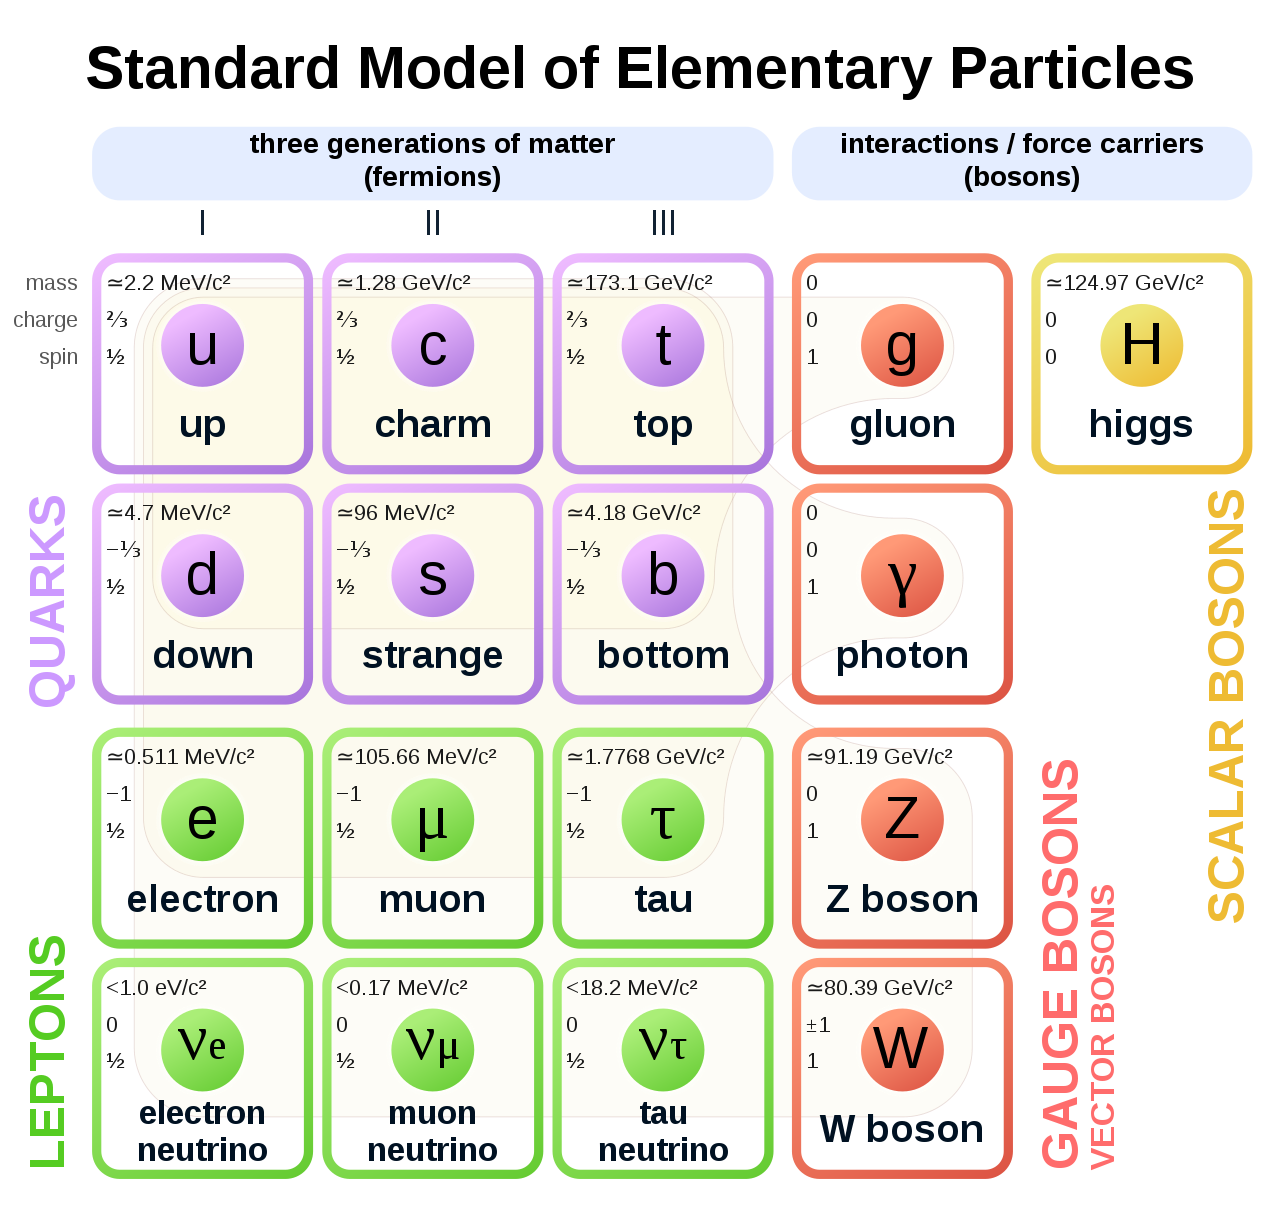
\includegraphics[width=\textwidth,keepaspectratio]{SMwiki.png}
		\caption{The list of particles that enters the \gls{sm}\cite{sm_wiki}. }
		\label{fig::SMwiki}
	\end{figure}
		
An important feature of the \gls{qft} is that particles also interact with physical vacuum. For instance, a charged particle polarizes the physical vacuum, so the vacuum changes the charge of the particle~\cite{Schwinger_polariz}.This interaction with virtual particles depends on the energy scale and so do the observed quantities like charge, mass etc. The \gls{sm} is able to predict parameter evolution, so if the value of a certain input parameter $q_0$ is known at the energy $\Lambda_0$ then it is possible to predict its measurable value $q$ at the energy $\Lambda$. This changing of physical parameters is an integral part of the \gls{qft} and is called \textit{renormalisation} \cite{bogol}, \cite{Glashow:1959wxa}. In the Figure \ref{fig::running} the dependence of the inverted \gls{sm} coupling constants on the energy is shown. 

	 \begin{figure}[htpb]
	 	\centering
	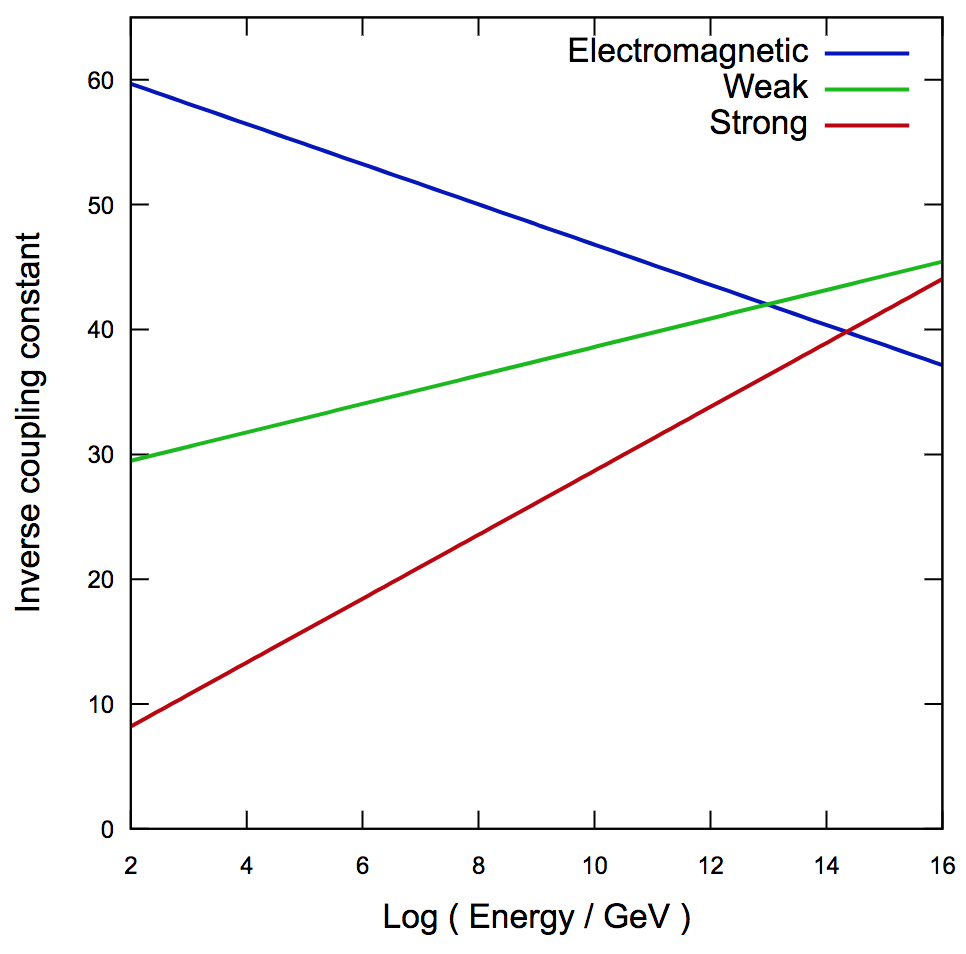
\includegraphics[width=0.6\textwidth,keepaspectratio]{coup_const.png}
	\caption{The running of the inverted \gls{sm} coupling constants \cite{coupl_wiki}. }
	\label{fig::running}
	\end{figure}
As we can see from picture \ref{fig::running} the strong coupling constant is decreasing with the energy. This phenomenon is called \textit{the asymptotic freedom} \cite{Gross,Politzer,Vanyashin}.



\section{Classical fields and gauge invariance principle}
\label{sec::gauge}
A consistent mathematical description of fields appears to be a more challenging task compared to the description of physical objects that have a definite size and shape even in the classical case. The derivation of Maxwell's equations has been a great success and allowed to obtain the first equations of motion of relativistic fields. It has also subseqently led to the understanding of special relativity \cite{einstein,poincare,lorentz}. Although for a more general case of fields other than electromagnetic it would be very useful to adopt a more systematic approach like that of Lagrangian or Hamiltonian in classical mechanics. 

It has turned out that for the relativistic case the Hamiltonian approach was not quite convenient, as the dedicated role of time over other degrees of freedom was in discord with relativistic space-time unification. However it was found possible to describe the fields within the Lagrangian approach. In classic mechanics the action of a mechanical system of $i$ mechanical objects is defined as:
 \begin{equation}
\nonumber
S = \int Ldt = \int \left( \sum_i T_i - U_i \right) dt,
\end{equation}
where $T_i$ and $U_i$ are the kinetic and potential energies of the $i^{th}$ object. Considering that by definition a field exists in every point of space-time, we need to define the Lagrangian density such that $L = \int \mathcal{L}(\phi,\partial_{k}\phi,\dot\phi ) d^3x$, where $\phi$ is a field and $\partial_{k}\phi = \nabla\phi$ - the field gradient, $\partial_{k} = \frac{\partial}{\partial x^{k}}$,  k = 1, 2, 3. Here and further Latin indices run through (1, 2, 3) and are used to denote spatial coordinates, while Greek indices denote space-time coordinates and run though (0, 1, 2, 3). So the action would look like: 
 \begin{equation}
S = \int Ldt =\int \mathcal{L}(\phi,\partial_{\mu}\phi,\dot\phi ) d^4x,
\end{equation}
Now we may use the principle of least action to obtain the equations of motion using the Euler-Lagrange formalism. Let's check it with the example of electromagnetic fields. The Lagrangian density of electromagnetic fields in a vacuum can be written like:
 \begin{equation}
S = -\frac{1}{4}\int F^{\mu \nu}F_{\mu \nu}d^4x.
\end{equation}
The electromagnetic tensor can be defined in terms of electric and magnetic field intensities: $F_{i0}=-F_{0i} = E_i$, $F_{ij} = \epsilon_{ijk}H_k$, where $\epsilon_{ijk}$ is the anti-symmetric Levi-Civita symbol. Alternatively $F_{\mu \nu}$ can be defined in terms of the 4-potential $A_{\mu}$:
 \begin{equation}
F_{\mu \nu} = \partial_{\mu}A_{\nu} - \partial_{\nu}A_{\mu}.
\end{equation}
Now we can safely apply the variational principle, and putting $\delta S=0$ obtain the Maxwell equations in vacuum:
 \begin{equation}
\partial_{\mu}F_{\mu \nu} = 0.
\end{equation}
Noticing the symmetries of the system and using the Noether's theorem\cite{Noether1918} we can find the invariants of electromagnetic field. For example, translational symmetry in time and space ensures conservation of energy and momentum. Let's now consider a symmetry of a different kind. The field potential can be shifted by a gradient of an arbitrary function $\alpha=\alpha(x^\mu)$:

\begin{equation}
\begin{array}{lcl} 
A_{\mu}(x) \rightarrow A^{\prime}_{\mu}(x)  = A_{\mu}(x)+\partial_{\mu}\alpha(x)  \\ 
F_{\mu \nu} \rightarrow F^{\prime}_{\mu \nu}  = \partial_{\mu}(A_{\nu}(x)+\partial_{\nu}\alpha(x))-\partial_{\nu}(A_{\mu}(x)+\partial_{\mu}\alpha(x))=\partial_{\mu}A_{\nu} - \partial_{\nu}A_{\mu}=F_{\mu \nu},
\end{array} 
\end{equation}
where the commutativity of the derivative operator $\partial_{\mu}\partial_{\nu}\alpha(x)=\partial_{\nu}\partial_{\mu}\alpha(x)$ was used.
Let us now consider the electromagnetic theory in the presence of charges and currents:
 \begin{equation}
\mathcal{L} = -\frac{1}{4} F^{\mu \nu}F_{\mu \nu} + j^{\mu}A_{\mu}.
\end{equation}
Now we have an interaction of a field potential $A_{\mu}$ with 4-current $j^{\mu}=(-\rho,j^{i})$. It turns out to be a general property of the field theories: the only form of interaction allowed is between a gauge field and a current.  After applying the gradient field transformation and the least action principle we can obtain the corresponding conservation law:
\begin{equation}
\partial_{\mu}j^{\mu}=0.
\end{equation}
 So this gradient symmetry~\cite{bogol} or as it is called more often gauge symmetry is connected to the conservation of electric current. If a theory is invariant under gauge transformations then it is called a gauge invariant theory. As we have just seen electrodynamics is the simplest example of such a theory. Taking gauge symmetries into consideration \cite{YangMills} has played a huge role in the development of the \gls{sm}.
 
 Gauge degree of freedom can be constrained in arbitrary way by applying additional conditions on the gauge function. This is called fixing the gauge and becomes necessary for the quantization. As a result of a non-trivial procedure it can be show that any physical result must be gauge-invariant, i.e. must not depend on the gauge. 

\section{Quantum electrodynamics}
\label{sec::qed}
\gls{qed} is a theory of interaction between light and electrically charged particles. Historically it was the first quantum field theory to reach good agreement between quantum mechanics and special relativity. \gls{qed} vacuum has zero expectation value.  Nowadays it is considered to be one of the most precise physical theories ever: theory predictions and experiment results agree up to $~O(10^{-11})$. It has also served as a model for the composition of the subsequent parts of the \gls{sm}, describing other fundamental interactions. Let us consider the free Dirac field based Lagrangian:
 \begin{equation}
\mathcal{L} = \bar \psi(x) (i\slashed\partial - m)\psi(x),
\end{equation}
where $\psi$ and $\bar \psi$ are Dirac wave function and its complex conjugate respectively, $\slashed\partial \equiv \gamma_{\mu}\partial^{\mu}$, $\gamma_{\mu}$ is one of the four gamma-matrices and $m$ is the mass of the Dirac field. 
Such a theory, though, would not be physically consistent. This reflects the fact the quantum nature of spin and spinor fields have to be treated as quantum fields. For instance, an attempt to calculate the energy of a Dirac field would lead to a contradiction: the energy would not be positively defined, as some spinors would have negative energies. 

This Lagrangian has an internal symmetry to the U(1) transformation: $\psi\rightarrow e^{-i\alpha(x)}\psi$, \: $\bar\psi\rightarrow e^{i\alpha(x)}\bar\psi$. According to Noether's theorem this symmetry implies current conservation: $j^{\mu}=\bar\psi\gamma^{\mu}\psi$.
Now let's get the combined Lagrangian of electromagnetic and Dirac fields, adding the interaction term:
 \begin{equation}
\mathcal{L} = \mathcal{L}_{Dirac^{free}} + \mathcal{L}_{EM^{free}} + \mathcal{L}_{Interaction} = -\frac{1}{4} F^{\mu \nu}F_{\mu \nu}+\bar \psi(x) (i\slashed\partial -m)\psi(x) - q\bar\psi\gamma^{\mu}A_{\mu}\psi,
\end{equation}
where q represents the elementary electric charge. This Lagrangian above is gauge invariant and can be rewritten in a more convenient form:
 \begin{equation}
\mathcal{L} =  -\frac{1}{4} F^{\mu \nu}F_{\mu \nu}+\bar \psi(x) (i\slashed D -m)\psi(x),
\end{equation}
where $D_{\mu} = \partial_{\mu}-iqA_{\mu}$ is a covariant derivative. If one considers space-time in the presence of a field as curved, then $A_{\mu}$ would play a role of connectivity. It must be noted that values like $m$ and $q$ meaning electron mass and charge\footnote{Charge of the electron is related to the electromagnetic coupling constant.} are the \gls{sm} input parameters mentioned in \ref{sec::sm_gen}.  

Further calculations are to be performed by the means of the quantum field theory formalism that treats interaction terms like a perturbation to the free fields, making power series expansion in the coupling constant. In the case of electrodynamics the coupling constant is quite small so good precision is reached soon. Since the photons do not directly interact with other photons, \gls{qed} allows only one type of vertex - with two electron lines and one photon line. 

\begin{figure}
\label{fig::qed}
\centering
\feynmandiagram [horizontal=a to b, baseline=(current bounding box.center)] {
	i1 -- [fermion] a -- [photon] i2,
	a -- [fermion] b,
	f1 -- [photon] b -- [fermion] f2,
};
\feynmandiagram [horizontal=a to b, layered layout] {
	i1 -- [fermion] a,
	a -- [photon, half left] b,
	a -- [fermion] b,
	b -- [fermion] f1,
};
\feynmandiagram [horizontal=a to b,  layered layout, baseline=(b)] {
	i1 -- [photon] a,
	a -- [fermion, half left] b,
	b -- [fermion, half left] a,
	b -- [photon] f1,
};
\caption{Examples of QED diagrams: Compton scattering, electron self-energy, photon self-energy.}
\end{figure}
Although the tree-level processes and diagrams were well understood by 1930th, the loop diagrams were properly explained only by the end of the 1940th making it possible to obtain numerical results of the higher orders of power series expansion and achieve higher precision predictions for QED processes~\cite{Schwinger_polariz,Schwinger_covar,Feynman_math,Feynman_positrons,Feynman_spacetime,Tomonaga,Dyson_all,Dyson_smatr}. The examples of QED diagrams are presented in figures below.

It must be noted that although immediate photon-photon interaction is impossible, light-by-light scattering is still possible through loops:\\

\begin{center}

\feynmandiagram[layered layout, horizontal=a to b] {
	% Draw the top and bottom lines
	i1 
	-- [photon, edge label = \( \gamma \)] a
	-- [fermion, edge label=\(e \)] b
	-- [photon, edge label=\( \gamma \)] f1 ,
	i2 
	-- [photon, edge label=\( \gamma \)]  c
	-- [anti fermion, edge label=\(e \)]  d
	-- [photon, edge label=\( \gamma \)]  f2,
	%Draw the two internal fermion lines
	{ [same layer] a -- [anti fermion, edge label =\(e\)] c },
	{ [same layer] b -- [fermion, edge label=\(e\)] d},
};\\
\end{center}
This process was theoretically described in 1936~\cite{lbl_th} and experimentally observed 83 years after in heavy ion collisions at the LHC \cite{lbl_exp}.
\section{Electroweak theory and the Higgs mechanism}
All the fermions of the standard model are subject to the weak interaction, so its importance for physical processes can not be underestimated. At low energy the weak interaction manifests itself mainly through flavour-changing decays like beta-decay and muon decay. The electroweak theory was created in the end of 1950s~\cite{Glashow:1959wxa} \cite{weinberg} \cite{Salam1959} thanks to numerous experimental results that allowed to shape its properties. The theory assumed that the electromagnetic and weak fundamental forces are actually manifestation of the same gauge group that has a gauge symmetry $SU(2)_L \cross U(1)$ with massive charged and neutral bosons. A few years later the structure of electroweak vacuum was explained along with the mechanism that has allowed the bosons to gain mass \cite{brout}, \cite{higgs}. Assuming this the Lagrangian of the electroweak theory must consist of three parts~\cite{Hollik_2006}: 
\begin{itemize}
	\item Gauge fields that would mediate the interaction.
	\item Fermions that interact with gauge fields
	\item A scalar Higgs field with non-zero vacuum energy that breaks the $SU(2)_L$ symmetry and couples to the fermions.
\end{itemize}
 \begin{equation}
\mathcal{L}_{EW} = \mathcal{L}_{Gauge} +\mathcal{L}_{Higgs} +\mathcal{L}_{Fermions}
\end{equation}
\subsection{Electroweak gauge fields}
\label{sec::ewk}
As it was already pointed out before, knowing the symmetries of a physical system allows one to compose the gauge fields Lagrangian. The part with U(1) symmetry would look like the electromagnetic field from \ref{sec::gauge} having the hypercharge $Y$, a vector potential $B_{\mu}$ and a gauge coupling $g_1$. The SU(2) field would have 3 vector components $W^{1,2,3}_{\mu}$, three isospin operators $I_1$,$I_2$,$I_3$ and a gauge coupling $g_2$. We can pick the Pauli matrices $\sigma^{i}$ as the representation of generators of the SU(2) group, then the structure constants are $\epsilon_{abc}$ - Levi-Civita symbol.
\begin{equation}
\begin{array}{lcl} 
\mathcal{L_{G}} =  -\frac{1}{4}B_{\mu \nu}B^{\mu \nu} -\frac{1}{4}W^a_{\mu \nu}W^{\mu \nu,a} 
B_{\mu \nu}  =\partial_{\mu}B_{\nu} - \partial_{\nu}B_{\mu}\\ 
W^a_{\mu \nu}  =\partial_{\mu}W_{\nu} - \partial_{\nu}W_{\mu}+g_2\epsilon_{abc}W^b_{\mu}W^c_{\nu},\\ 
\end{array} 
\end{equation}
where the term $g_2\epsilon_{abc}W^b_{\mu}W^c_{\nu}$ appears due to the non-Abelian nature of the SU(2) group (the generators don't commute).


\subsection{Fermion sector}
Each fermion generation expressed as left-handed doublet and right-handed singlets is a fundamental representation of the group $SU(2) \times U(1)$:
\begin{align}
\begin{pmatrix}
\nu_e  \\
e \\
\end{pmatrix}_L,
\begin{pmatrix}
e_R \\
\end{pmatrix},
\begin{pmatrix}
u \\
d \\
\end{pmatrix}_L,
\begin{pmatrix}
u_R \\
\end{pmatrix},
\begin{pmatrix}
d_R \\
\end{pmatrix},
\end{align}

\begin{align}
\begin{pmatrix}
\nu_\mu  \\
\mu \\
\end{pmatrix}_L,
\begin{pmatrix}
\mu_R \\
\end{pmatrix},
\begin{pmatrix}
s \\
c \\
\end{pmatrix}_L,
\begin{pmatrix}
s_R \\
\end{pmatrix},
\begin{pmatrix}
c_R \\
\end{pmatrix},
\end{align}

\begin{align}
\begin{pmatrix}
\nu_\tau  \\
\tau \\
\end{pmatrix}_L,
\begin{pmatrix}
\tau_R \\
\end{pmatrix},
\begin{pmatrix}
b \\
t \\
\end{pmatrix}_L,
\begin{pmatrix}
b_R \\
\end{pmatrix},
\begin{pmatrix}
t_R \\
\end{pmatrix}.
\end{align}

Their quantum states are classified using the following quantum numbers: weak isospin $I_3$, $Q$, weak hypercharge $Y$. Their electric charge can be obtained using the Gell-Mann-Nishijima relation:
  \begin{equation}
Q = I_3+\frac{Y}{2}.
\end{equation}

The fermions are divided by their chirality: only the left-handed particles take part in the charged current of the weak interaction. The left-handed fermion fields of each lepton and quark generation j
  \begin{equation}
    \psi^L_j = \begin{pmatrix}
	\psi^L_{j+}  \\
	\psi^L_{j-}  \\
\end{pmatrix}
  \end{equation}
make SU(2) doublets, with indices $\sigma=\pm$, while the right-handed fermions can be written as singlets:
 \begin{equation}
\psi^R_j = \psi^L_{j\sigma}.  
\end{equation}
Like in the the electromagnetic case we can define the covariant derivative that would ensure the gauge invariance of the Lagrangian:
 \begin{equation}
D_\mu = \partial_{\mu} - ig_2I_aW^a_{\mu}+ig_1\frac{Y}{2}B_{\mu},
\end{equation}
with $I_a \equiv \frac{\sigma_a}{2}$, then fermion Lagrangian takes the following form:
 \begin{equation}
\mathcal{L}_{Fermions} = \sum_f \bar \psi^L_j i \gamma^{\mu}D_{\mu}\psi^L_j +\sum_{f,\sigma} \bar \psi^R_{f,\sigma}  i \gamma^{\mu}D_{\mu}\psi^R_{f,\sigma}  .
\end{equation}

\subsection{Higgs field breaking the symmetry}
\label{sec:symmetry_breaking}
The Higgs field is represented by single complex a scalar doublet field $\Phi(x)$, that has 4 independent components. It spontaneously breaks the  $SU(2)\times U(1)$ gauge symmetry, leaving the $U(1)_{EM}$ symmetry intact. The Higgs field doublet has the hypercharge $Y=1$:
  \begin{equation}
\Phi(x) = \begin{pmatrix}
\phi^{+}(x)  \\
\phi^{0}(x)  \\
\end{pmatrix}.
\end{equation}
The Higgs field Lagrangian with non-zero vacuum expectation value is: 
 \begin{equation}
\mathcal{L}_{Higgs} = (D_{\mu}\Phi)^+(D_{\mu}\Phi)-V(\Phi)+\mathcal{L}_{Yukawa}.
\end{equation}
The gauge invariance of the Higgs Lagrangian is ensured in the traditional way by using the covariant derivative:
 \begin{equation}
D_{\mu} = \partial_{\mu} - ig_2I_aW^a_{\mu}+i\frac{g_1}{2}B_{\mu}.
\end{equation}
The Higgs potential contains the mass term and quartic self-interaction:
 \begin{equation}
V(\Phi) = -\mu^2 \Phi^+\Phi + \frac{\lambda}{4}\partial_{\mu}(\Phi^+\Phi)^2,
\end{equation}
where $\lambda$ stands for the quartic Higgs self-coupling constant and $\mu$ is the mass of the $\Phi$ field. The vacuum expectation value $<\Phi>$ does not vanish:
  \begin{equation}
<\Phi(x)> = \frac{1}{\sqrt(2)}\begin{pmatrix}
0  \\
v \\
\end{pmatrix},\;\;\;\;\; 
v = \frac{2\mu}{\sqrt(\lambda)}.
\end{equation}
Applying the unitarity gauge \cite{weinberg2} we can constrain three out of four degrees of freedom of the Higgs field and rewrite the Higgs doublet in the following way:
  \begin{equation}
 \Phi(x) = \frac{1}{2}\begin{pmatrix}
 	0 \\
 	v+H(x)  \\
 \end{pmatrix},
  \end{equation}
  which leaves us with a physical real neutral scalar field $H(x)$ with 
    \begin{equation}
	M_H=\sqrt{2}\mu.
  \end{equation}
 This real field would couple to itself forming triple and quartic self-coupling vertices, to the gauge fields through the covariant derivatives and to the charged fermions, giving them mass. The Yukawa term in Lagrangian the unitary gauge is:
     \begin{equation}
\mathcal{L}_{Yukawa}=-\sum_f m_f \bar\psi_f\psi_f-\sum_f \frac{m_f}{v} \bar\psi_f\psi_f H,
 \end{equation}
where
\begin{equation}
m_f=g_f\frac{v}{\sqrt{2}}=\sqrt{2}\frac{g_f}{g_2}M_W.
\end{equation}
The Higgs coupling constants to the corresponding fermion flavour are denoted as $g_f$. 
\subsection{Physical interpretation of gauge fields and parameters}
The Higgs coupling to the gauge fields results in the following terms in the Lagrangian:
\begin{equation}
\label{eq::weak_basis}
\frac{1}{2}\frac{g_2^2}{2}v^2(W_1^2+W^2_2)+\frac{v^2}{4}(W^3_{\mu},B_{\mu}) \begin{pmatrix}
g_2^2  & g_1 g_2 \\
g_1 g_2 & g_1^2   \\
\end{pmatrix}
\begin{pmatrix}
W^3_{\mu} \\
B_{\mu}   \\
\end{pmatrix}.
\end{equation}
In order to get the physical meaning of this expression let us make a transition to the basis of physical fields:
\begin{equation}
\begin{array}{lcl} 
W^{\pm}_{\mu}  &=& \frac{1}{\sqrt{2}}(W^{\mp}_{\mu}\mp iW^{\mp}_{\mu})\\ 
\begin{pmatrix} Z_{\mu} \\ A_{\mu}   \\ \end{pmatrix}  &=& \begin{pmatrix} \cos{\theta_{W}} & \sin{\theta_{W}}\\ -\sin{\theta_{W}}& cos{\theta_{W}}   \\ \end{pmatrix} \begin{pmatrix} W^3_{\mu} \\ B_{\mu}   \\ \end{pmatrix},
\end{array} 
\end{equation}
where $\theta_{W}$ is called the weak mixing angle or the Weinberg angle. In the new basis expression \ref{eq::weak_basis} has transparent physical sense:
\begin{equation}
M^2_W W^+_{\mu}W^{-\mu} +\frac{1}{2} (A_{\mu},Z_{\mu})\begin{pmatrix}
0 & 0 \\
0 & M^2_Z   \\
\end{pmatrix}
\begin{pmatrix}
A_{\mu} \\
Z_{\mu}   \\
\end{pmatrix},
\end{equation}
with
\begin{equation}
\begin{array}{lll} 
M_W &= & \frac{1}{2} g_2 v\\ 
M_Z &=& \frac{1}{2} \sqrt{g_1^2+g_2^2} v.
\end{array} 
\end{equation}
The mixing angle $\theta_W$ also has a very clear physical meaning:
\begin{equation}
\cos{\theta_W}=\frac{g_2}{g_1^2+g_2^2}=\frac{M_W}{M_Z}.
\end{equation}
With $A_{\mu}$ having a sense of electromagnetic potential its coupling to the electron must have a physical meaning of the electric charge $e=\sqrt{4\pi\alpha}$ we can express $e$ in terms of gauge couplings:
\begin{equation}
e=\frac{g_1 g_2}{g_1^2+g_2^2}, \;\;\;\;g_2=\frac{e}{\sin{\theta_W}},\;g_1=\frac{e}{\cos{\theta_W}} .
\end{equation}
Thus the demonstrated Weinberg rotation (see Fig. \ref{fig::weiberg_rotation}) replaces the original parameters $g_1$, $g_2$, $\lambda$, $\mu^2$, $g_f$ by another set of measurable values $e$, $M_W$, $M_Z$, $M_H$, $m_f$ which are the input parameters of the \gls{sm}.


\begin{figure}[htpb]
	\centering
	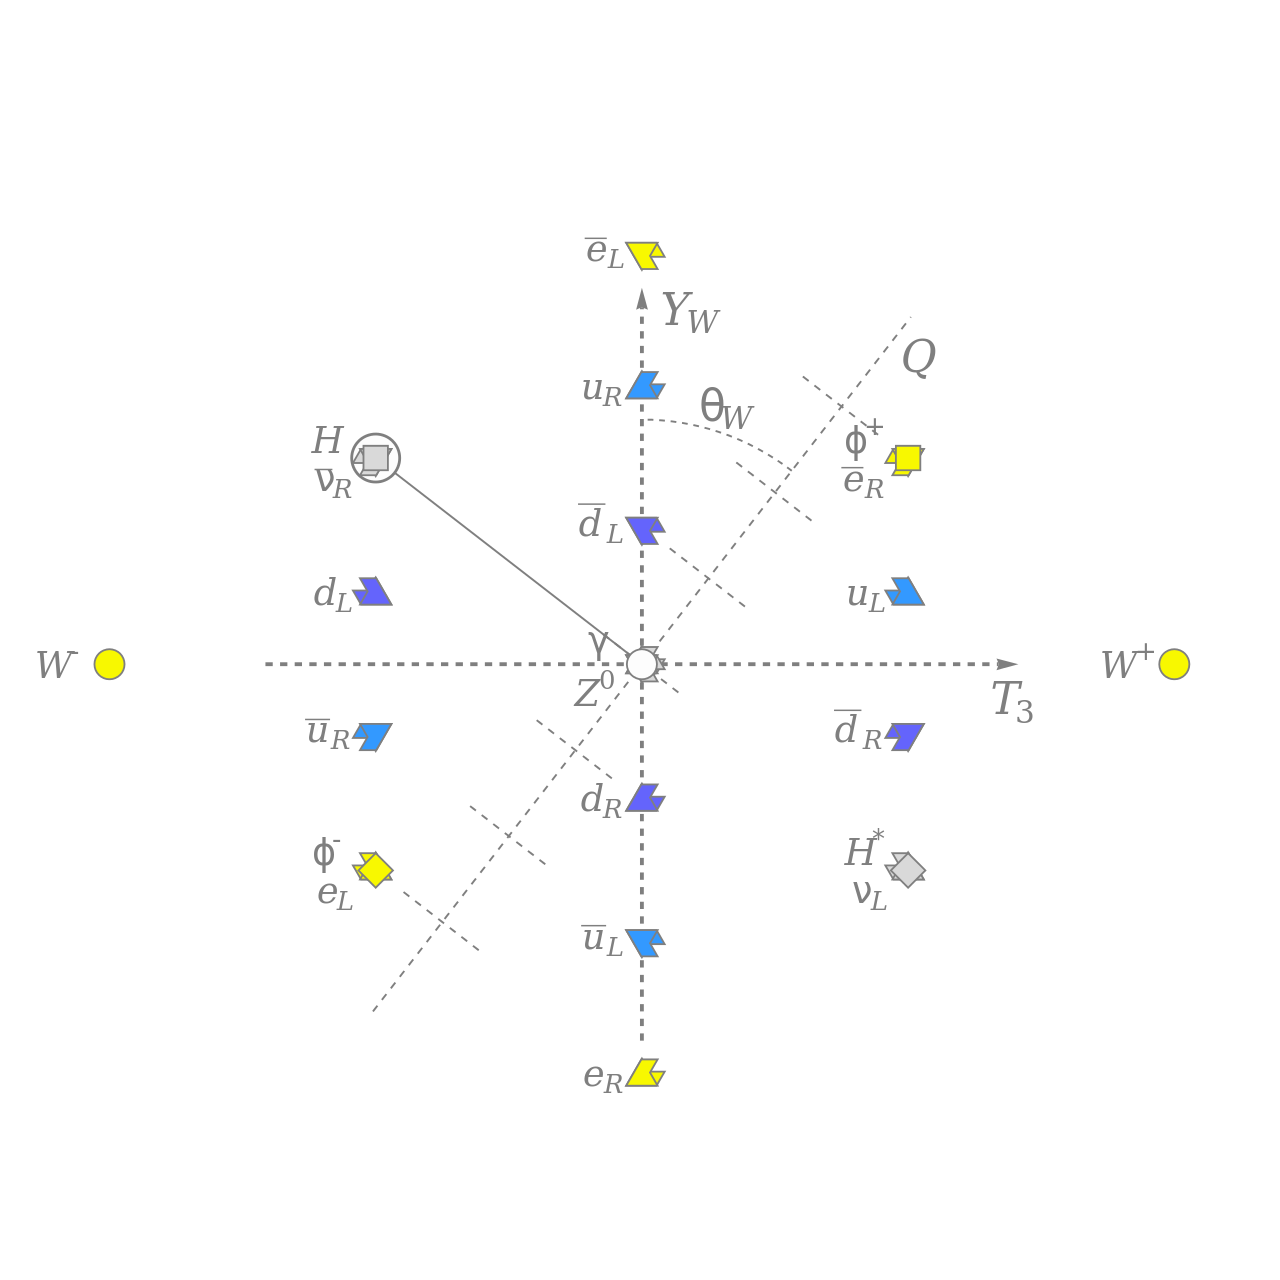
\includegraphics[width=0.65\textwidth,keepaspectratio]{weinb.png}
	\caption{Electroweak sector and the Weinberg rotation \cite{coupl_wiki}. }
	\label{fig::weiberg_rotation}
\end{figure}

\section{Chromodynamics}
\gls{qcd} is a non-Abelian gauge theory that describes strong interaction. \gls{qcd} is symmetric under unbroken SU(3) colour symmetry, so the interaction scheme is built in the same way as electromagnetic and electroweak theories. To preserve the gauge invariance the gauge field of gluons is introduced with 8 components, since SU(N) group has $N^2-1$ independent elements. The gluons are massless vector bosons like the photons, although because of the non-Abelian nature of the gauge group they couple not only to the fermions but also to the other gluons. The gauge invariant QCD Lagrangian with kinetic term containing covariant derivative would look like:
\begin{equation}
\begin{array}{lll} 
	\mathcal{L}_{QCD} &=& -\frac{1}{4}F^a_{\mu\nu}F_a^{\mu\nu} + \bar\psi_a(i(\gamma^{\mu}D_{\mu})^{ab} - m\delta^{ab})\psi_b,\\
	F^a_{\mu\nu}  &=& \partial_{\mu}A_{\nu}^a-\partial_{\nu}A^a_{\mu}+g_sf^{abc}A^b_{\mu}A^c_{\nu},\\
	D_{\mu} &=& \partial_{\mu} + ig_s A_{\mu}^at_a.
\end{array} 
\end{equation}
with $\psi$ being the quark field, m is the mass of the quark, a,b = 1, 2, ..., 8 are the colour indices, $g_s$ is the strong coupling constant, $f^{abc}$ are the structure constants of the SU(3) group and $t_a$ are the generators of the SU(3) group. \\
As it was already mentioned in \ref{sec::qed} quantitative calculations in \gls{qft} treat particle interaction as a perturbation to the free field theory. The coupling constant is considered to be a small parameter so every next power of the coupling constant is much smaller than the previous one. Due to asymptotic freedom the constant $\alpha_s$ becomes small at higher energies and allows perturbative calculations. But at a certain energy scale called $\Lambda_{QCD}\approx200$ MeV, \gls{qcd} becomes non-perturbative. It means we may no longer assume that interaction is a small perturbation of the free fields. This phenomenon causes the \textit{colour confinement}.

	 \begin{figure}[htpb]
	 	\centering
	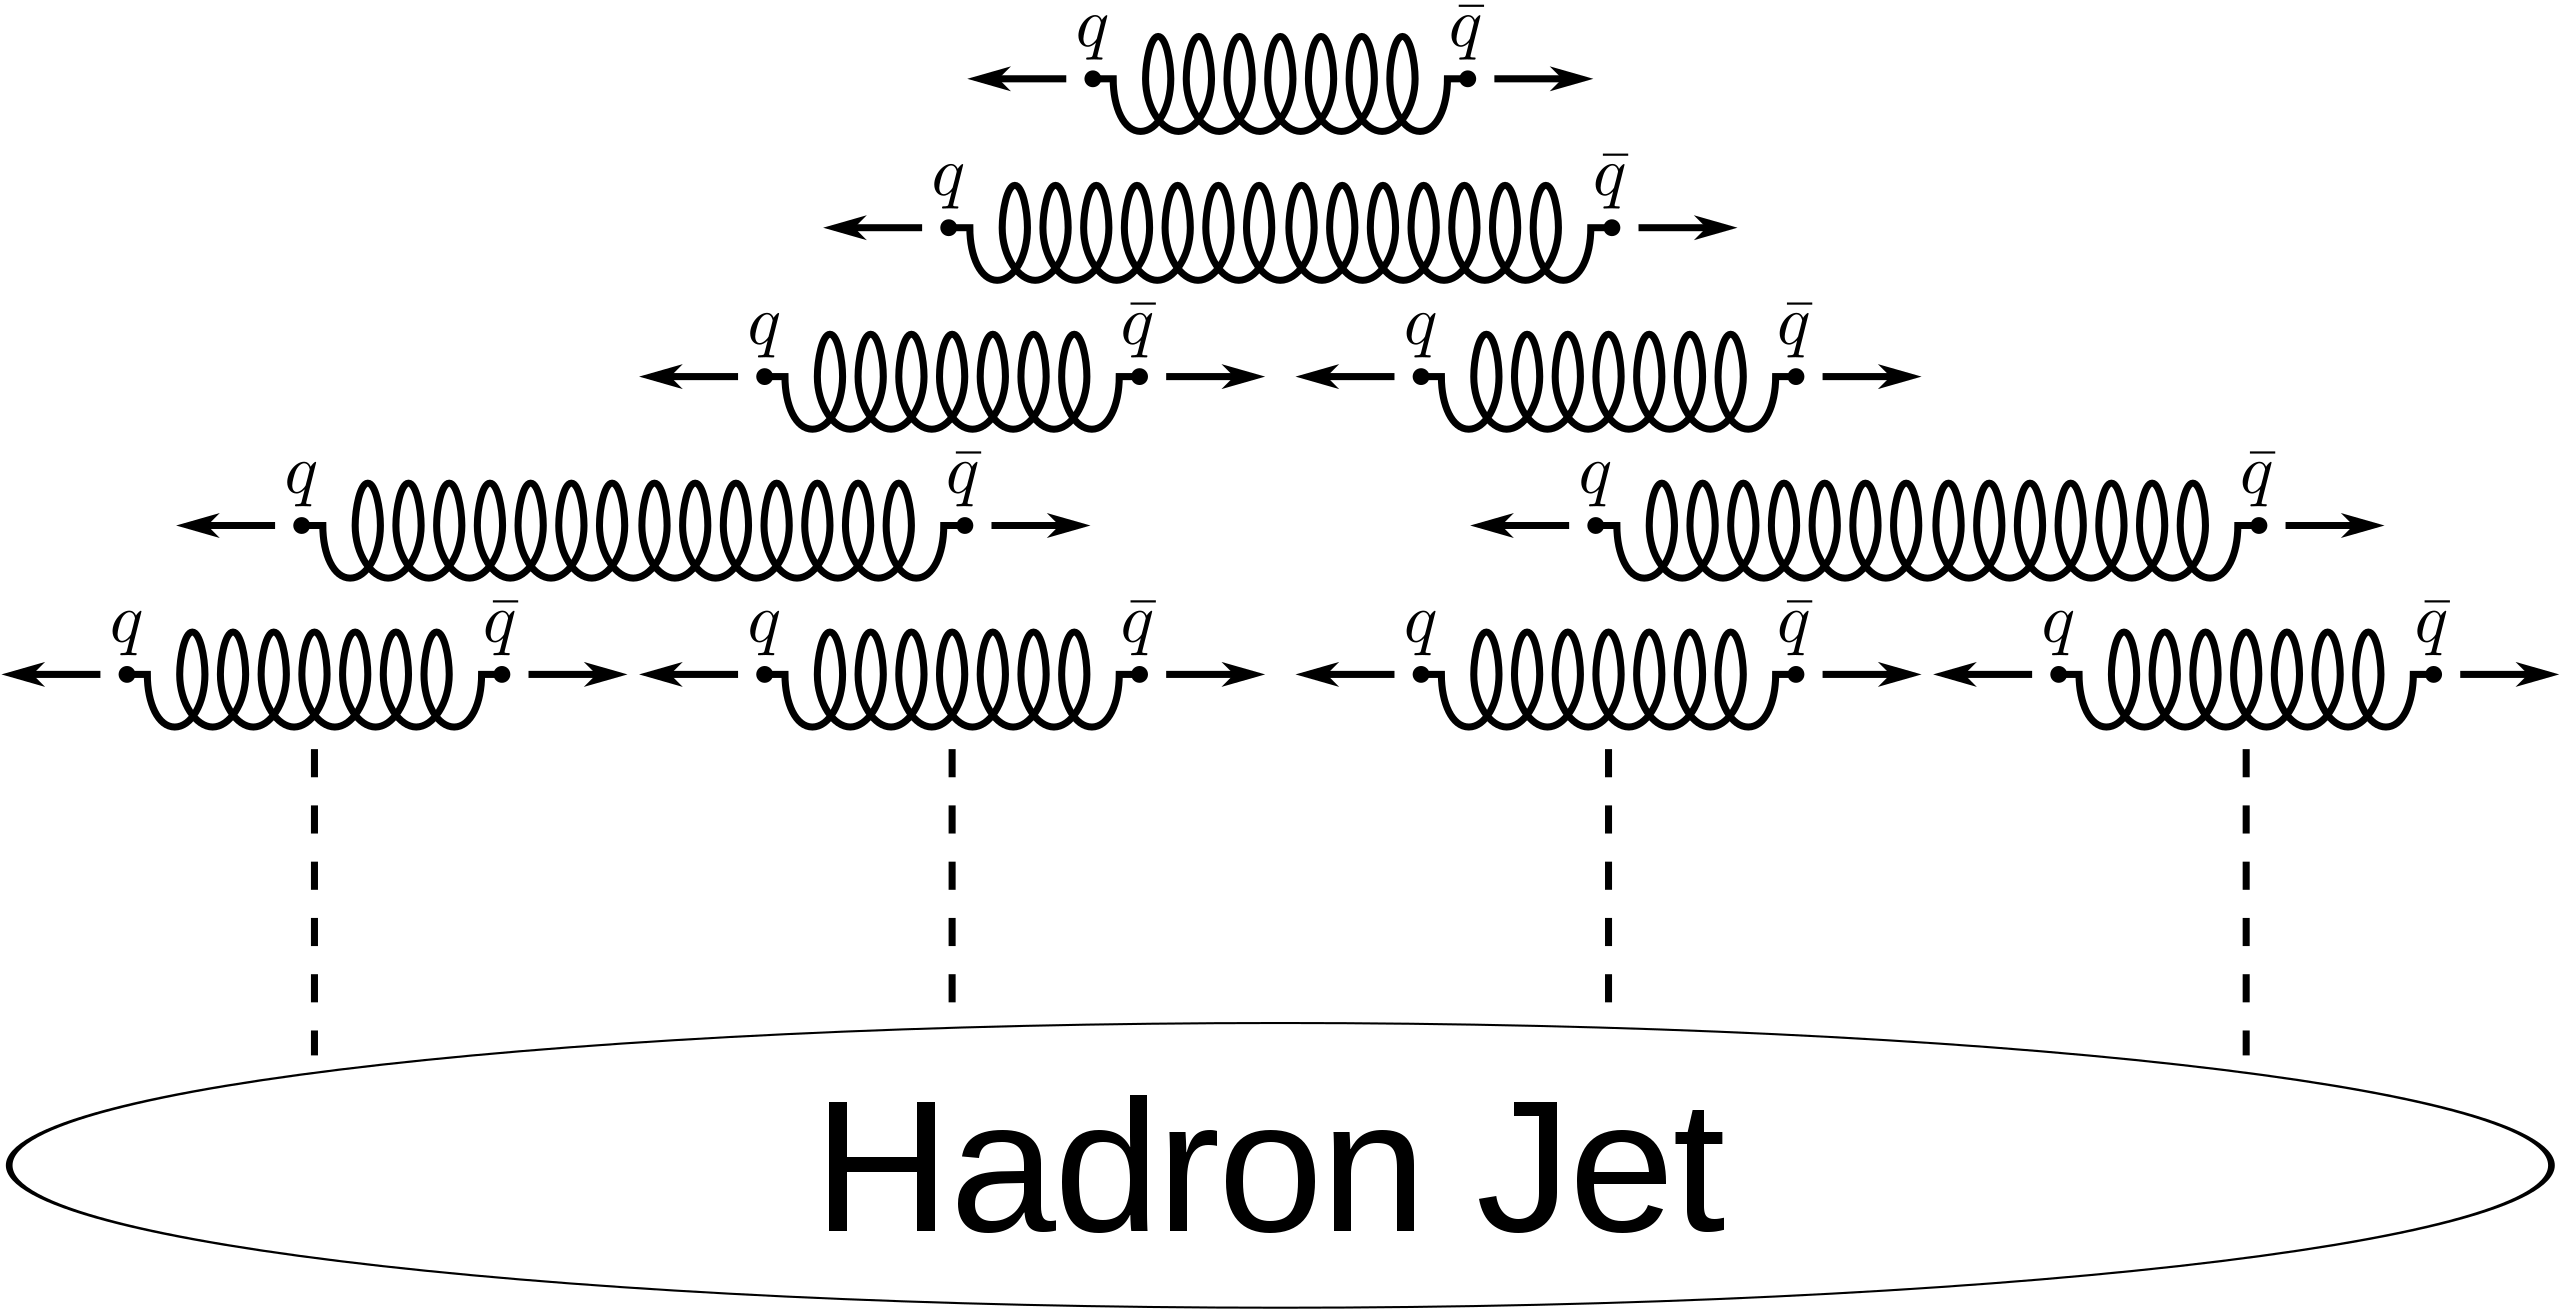
\includegraphics[width=0.75\textwidth,keepaspectratio]{confinement.png}
	\caption{The formation of a hadron jet \cite{conf_wiki}. }
	\label{fig::jet}
	\end{figure}
Because of colour confinement we can only observe colourless objects like baryons and mesons, but not quarks and gluons. If a high-energetic parton gets torn out of a hadron then it creates an avalanche-like process creating quark-antiquark pairs until it fully hadronizes (see Fig. \ref{fig::jet}) neutralizing its colour. Such an avalanche is called a hadronic jet. 

Currently there is no viable physical theory that would describe \gls{qcd} vacuum and low-energy behaviour of quarks and gluons. This also means that although nuclear forces are evidently residuals of the QCD interaction of partons within the baryons, there is no continuity between \gls{qcd} and nuclear physics. Confinement and low-energy \gls{qcd} remain an unsolved problem of modern physics. 



\newpage
\chapter{The Large Hadron Collider}
    \chapterprecishere{
        ``Potentielle citation sans aucun rapport avec le sujet"\par\raggedleft--- \textup{Personne inconnue}, contexte à déterminer
    }
    
   
        
    \section{Introduction}
    
        The study of elementary particles naturally demands a stable source of particles. At the dawn of particle physics the two main sources were radioactive materials and the cosmic rays. However soon researchers became in need of a more reliable source of particles in terms of particle energy, luminosity and experimental repeatability. This has commenced the era of particle accelerators.\\
        The first examples of particle accelerators were designed in late 1920s and early 1930s. Two different designs emerged: linear and circular. The former accelerates particles via electric field during the single pass through the machine, while the latter uses magnetic field to make accelerated particles go in circles allowing to re-accelerate the same beam many times. On the other hand the circular design comprises energy losses due to Bremsstrahlung radiation.\\
        In the second half of the XX century the accelerators gradually got bigger and bigger in both size and center-of-mass energy of the accelerated particles. This has allowed to create an experimental basis for the development of modern particle physics, notably the Standard Model.\\
        Up to this day the biggest particle accelerator with the highest center-of-mass energy is the Large Hadron Collider (LHC). LHC is a circular collider that lies in a tunnel of 27 km under the French-Swiss border next to Geneva \cite{Bruening}. In 2012 two biggest experiments of LHC have claimed the discovery of the Higgs boson, the last elementary particle predicted by the Standard Model which was not yet discovered by that time. \cite{higgs_atlas}, \cite{higgs_cms}.
        
        \section{The principle of a circular collider}
        
        Circular colliders - how they work and why they are circular. Cyclotron frequency.
Pipes, dipoles, quadrupoles, RF cavities, interaction points.

        \section{The LHC acceleration sequence}
        A few sentences and pictures about the chain between a ballon of hydrogen and the collisions at the IPs. 

        \section{Bunching and luminosity }
How and why the beam is bunched. How the luminosity is delivered to the IP and why it is a very important observable

        \section{LHC performance during the low-mu run}
A few plots and tables containing info about the delivered and collected luminosity

\newpage
\chapter{The Large Hadron Collider}
   The chapter on the Large Hadron Collider provides a bit of overview on the purpose and operation principle of the collider. It also provides the information on the special low pile-up run which is the main source of experimental data for the W boson transverse momentum measurement analysis.
   
   
    \section{Introduction} 
        The study of elementary particles naturally demands a stable source of particles. At the dawn of particle physics the two main sources were radioactive materials and cosmic rays. However soon researchers became in need of a more reliable source of particles in terms of particle energy, luminosity and experimental repeatability. This has commenced the era of particle accelerators.\\
        The first examples of particle accelerators were designed in the late 1920s and in the early 1930s. Two different designs emerged: linear and circular. The former accelerates particles via electric field during the single pass through the machine, while the latter uses magnetic field to make accelerated particles go in circles allowing to re-accelerate the same beam many times. On the other hand the circular design comprises energy losses due to Bremsstrahlung radiation.\\
        In the second half of the XX$^{th}$ century the accelerators gradually got bigger and bigger in both size and centre-of-mass energy of the accelerated particles. This has allowed to create an experimental basis for the development of modern particle physics, notably the Standard Model.\\
        Up to this day the biggest particle accelerator with the highest centre-of-mass energy is the Large Hadron Collider (LHC). The LHC is a circular collider that lies in a tunnel of 27 km under the French-Swiss border next to Geneva \cite{Bruning:2668521}. In 2012 the two biggest experiments of LHC have claimed the discovery of the Higgs boson, the last elementary particle predicted by the Standard Model which was not yet discovered by that time. \cite{higgs_atlas}, \cite{higgs_cms}.
        
        \section{The LHC running sequence}
                   \begin{figure}[htpb]
        	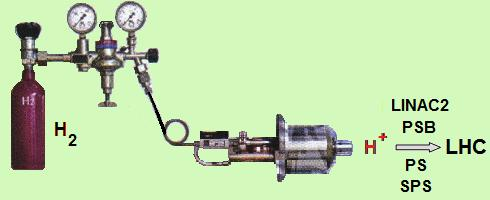
\includegraphics[width=\textwidth,keepaspectratio]{hydro_tank.jpg}
        	\caption{A hydrogen tank supplies LHC with protons \cite{hydro}.}
        	\label{fig::hydro}
        \end{figure}
        	
        It takes quite a journey for a proton to travel from a hydrogen tank (Fig. \ref{fig::hydro}) into one of the LHC's collision points. A resourceful system of pre-accelerators is necessary to make the proton beam ready to get injected into one of the two LHC beam pipes. The LHC accelerator complex was not built from scratch - it uses vast CERN infrastructure, that was built for the previous particle physics experiments. \\
        After stripping the electrons off the atoms of hydrogen using a magnetic field the yielded protons get accelerated to the energy of 50 MeV by the Linac 2\footnote{After Run 2 the Linac 2 has been decommissioned to be succeeded by Linac 4.} \cite{sequence}. After that the beam gets into the Proton Synchrotron Booster (PSB) to be accelerated to 1.4 GeV. The next link of the pre-acceleration chain is the Proton Synchrotron (PS) - a true veteran among CERN accelerators that first accelerated protons in 1959 breaking the world record in acceleration energy. Currently thanks to PSB and other modifications it can sustain proton beam intensity ~1000 times larger than back in 1959. The PS accelerates the beam up to 25 GeV and conveys it further to the Super Proton Synchrotron (SPS) - the second-largest particle accelerator at CERN. Back in 1983 the massive electroweak bosons were discovered at the SPS but even now it serves as a main accelerator for the NA61/SHINE, NA62 and COMPASS experiments. The SPS raises the beam energy to 450 GeV and finally injects it into the LHC beam pipes (see Fig \ref{fig::layout}).\\
   

	\begin{figure}[htbp]
	\begin{subfigure}[t]{0.48\textwidth}
		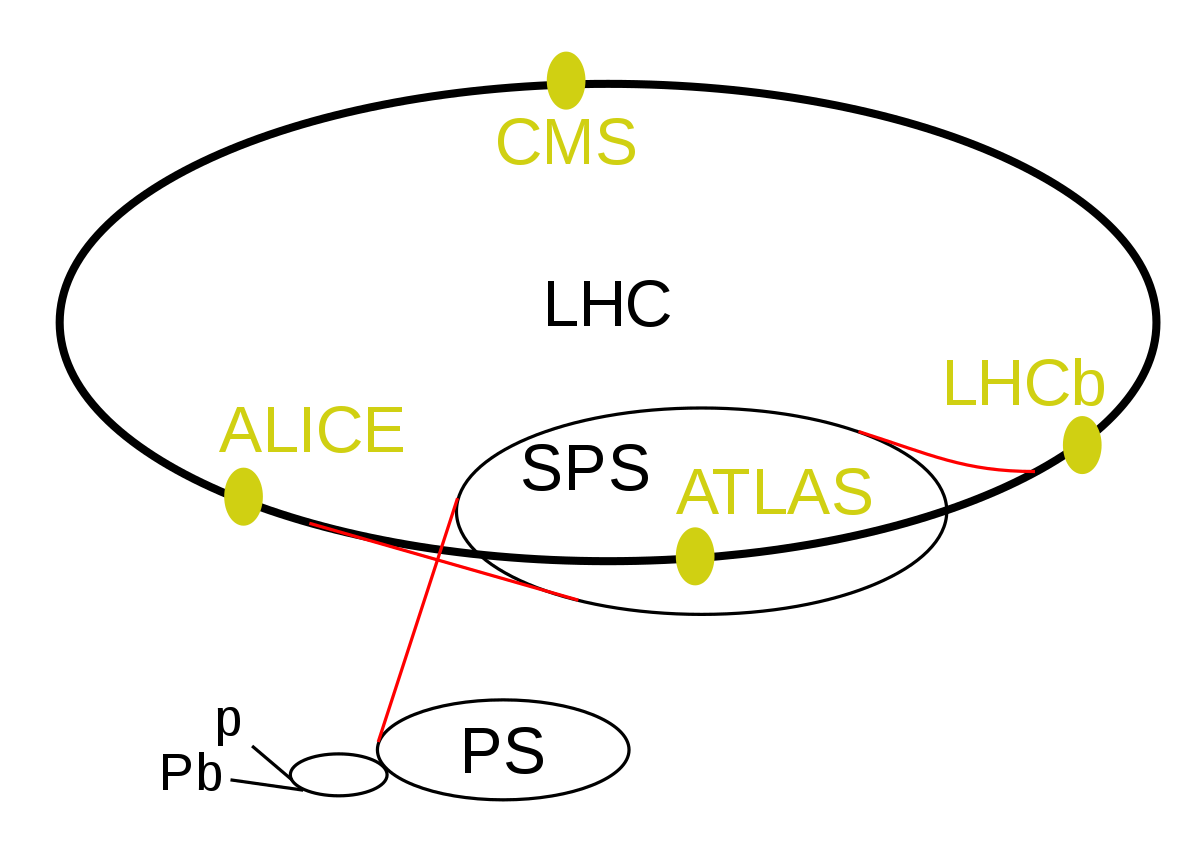
\includegraphics[width=\textwidth,keepaspectratio]{LHC.png}
		\caption[Acceleration sequence]{Acceleration sequence \cite{sequence}.}
		\label{fig::seq}
	\end{subfigure}
	\hfill
	\begin{subfigure}[t]{0.48\textwidth}
		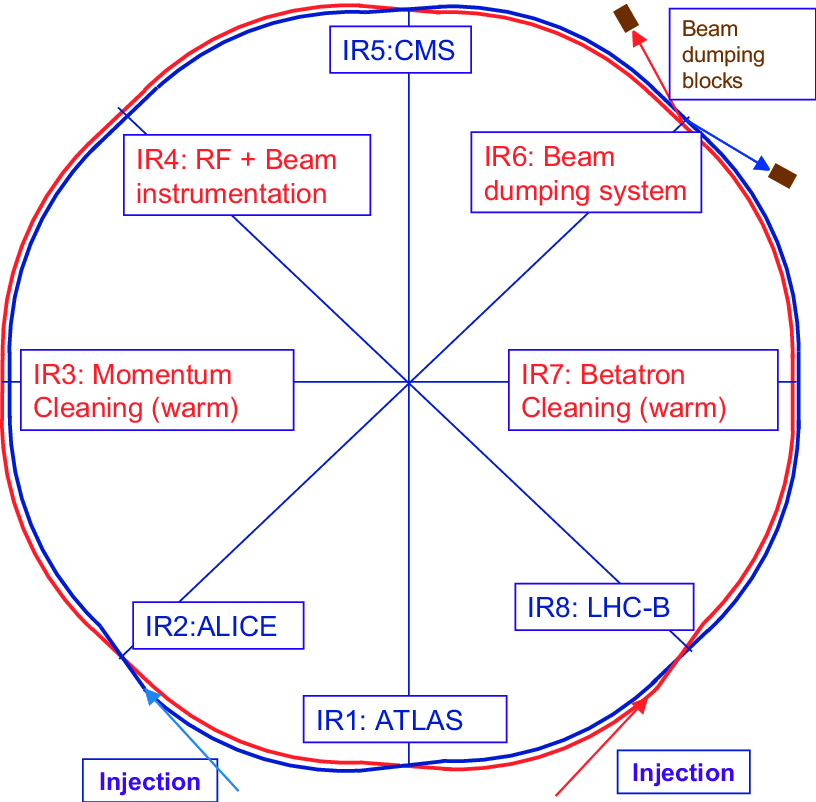
\includegraphics[width=\textwidth,keepaspectratio]{Layout.png}
		\caption[Beam pipes]{LHC beam pipes and crossing points.}
		\label{fig::pipes}
	\end{subfigure}
	\caption{Schematic depiction of the LHC ring.}
	\label{fig::layout}
\end{figure}

     The LHC has inherited its 27 km tunnel from the predecessor, an electron-positron collider called Large Electron-Positron (LEP). However, all the LEP hardware has been replaced to sustain the conditions of the LHC beam. About 2/3 of the LHC circumference length is occupied by the dipole magnets that bend the trajectory of the proton beam to keep it within the pipe. These magnets use superconducting coils that conduct a current of 11080 amperes to produce a magnetic field of 8.3 Tl.\\
     Proton acceleration is maintained by the radio-frequency (RF) cavities (Fig. \ref{fig::rf_cavities}). Besides the acceleration particles the RF cavities are also responsible for beam bunching i.e. separating the beam into a train of separated particle packs, each containing about $10^{11}$ protons. During LHC Run 2 the bunches were separated by 7 meters (25 ns) with a maximum of 2556 circulating bunches.
	\begin{figure}[htbp]
	\begin{subfigure}[t]{0.48\textwidth}
		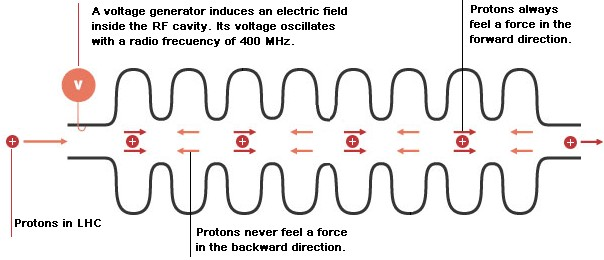
\includegraphics[width=\textwidth,keepaspectratio]{rf_cavities.jpg}
		\caption[RF Cavities]{The RF cavities \cite{rf_cavities}.}
		\label{fig::rf_cavities}
	\end{subfigure}
	\hfill
	\begin{subfigure}[t]{0.48\textwidth}
		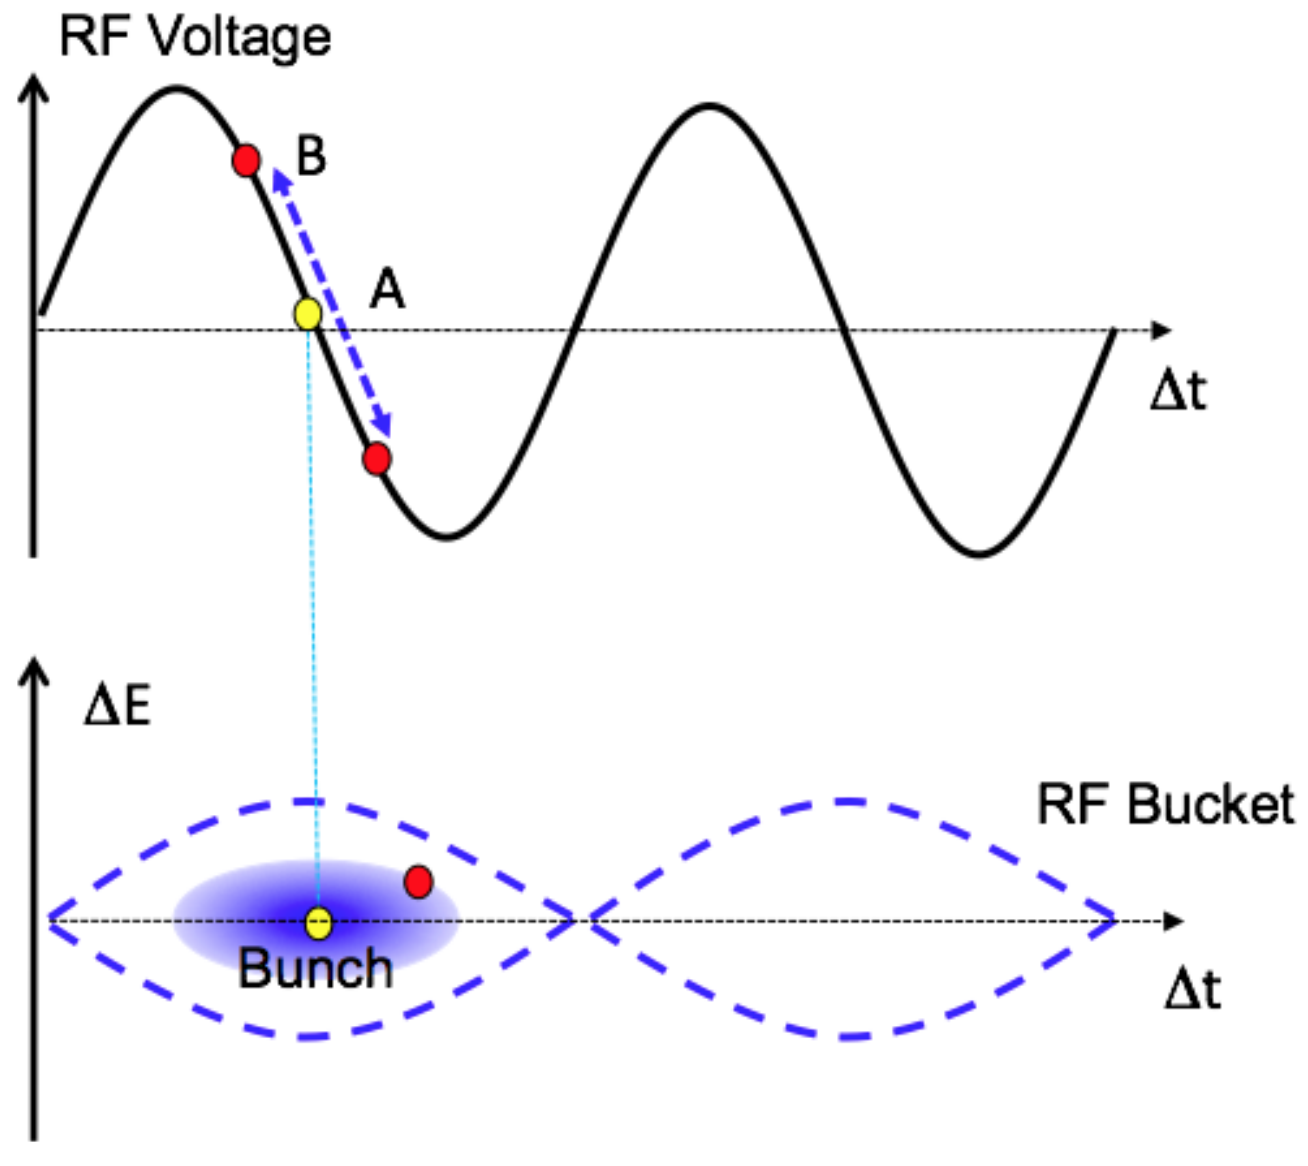
\includegraphics[width=\textwidth,keepaspectratio]{bunch0.png}
		\caption[Beam pipes]{Bunch behaviour at the RF cavities \cite{Wilson:513326}.}
		\label{fig::bunching}
	\end{subfigure}
	\caption{Bunching at RF cavities}
	\label{fig::bunch_at_rf}
\end{figure}
	The LHC has four crossing points, where the two beams are crossed in order to collide protons. Naturally, the particle detectors are installed at these four points. Before getting directed at the crossing point the beams get squeezed to make their cross-section as small as 16 $\mu m^2$ (Fig \ref{fig::2beams}).  	

	\begin{figure}[htbp]
	\begin{subfigure}[t]{0.48\textwidth}
		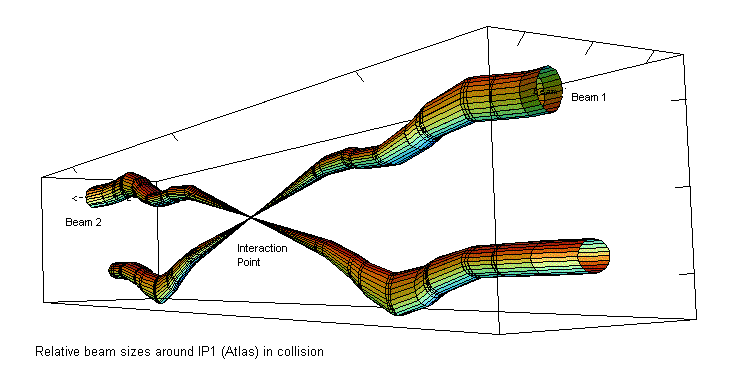
\includegraphics[width=\textwidth,keepaspectratio]{2-beams-IP.png}
		\caption[Two beams]{The two beams getting squeezed at the IP \cite{2beams}.}
		\label{fig::2beams}
	\end{subfigure}
	\hfill
	\begin{subfigure}[t]{0.48\textwidth}
		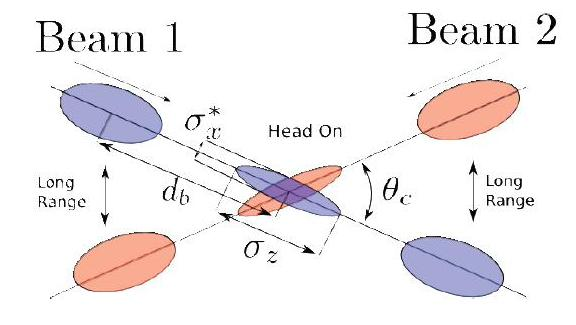
\includegraphics[width=\textwidth,keepaspectratio]{bunch_crossing.jpg}
		\caption[Bunches colliding]{Bunches at the collision point \cite{collisions}.}
		\label{fig::bunches_collision}
	\end{subfigure}
	\caption{Bunch crossing at the LHC.}
	\label{fig::interaction_point}
	\end{figure}
	In order to estimate the number of single proton-proton interactions in the crossing beams a value called instantaneous luminosity (simply called luminosity) is introduced. It is the proportionality factor between the number of events per second $dR/dt$ and the cross-section $\sigma_p$:
	 \begin{equation}
	\nonumber
	\frac{dR}{dt} = \mathcal{L} \cdot \sigma_p.
	\end{equation}
	For the case of head-on collisions the luminosity would equal to \cite{Lumi}:
	\begin{equation}
	\mathcal{L} = \frac{N_1N_2fN_b}{4\Pi \sigma_x \sigma_y},
	\end{equation}
	with $N_1$ and $N_2$ being the intensities of the two colliding beams, $f$ is the revolution frequency, $N_b$ - the number of bunches per beam, $ \sigma_x,\sigma_y$ - the r.m.s. beam widths in the corresponding dimensions, assuming that the bunches in both beams have the same size and Gaussian profiles. \\

	Head-on crossing of the beams would ensure maximal luminosity given the same beams, but on the other hand the measurement would suffer from unwanted beam-to-beam effects. To avoid it the beams at the LHC are crossed at an angle, which is called the crossing angle (see Fig. \ref{fig::bunches_collision}). 
	For the case of head-on collisions the luminosity gets a factor $\mathcal{F} $ \cite{Lumi}:
	\begin{equation}
	\mathcal{L} = \frac{N_1N_2fN_b}{4\Pi \sigma_x \sigma_y} \cdot \mathcal{F},\\
	\end{equation}
	with geometric factor
	\begin{equation}
	\nonumber
	\mathcal{F} = \frac{1}{\sqrt{ 1+\left(  \frac{\sigma_s}{\sigma_x}  \frac{\theta_c}{2} \right) }},
	\end{equation}
	where $\sigma_s$ is the r.m.s. of the bunch length and $\theta_c$ is the crossing angle. Varying the parameters like beam intensity, bunch spacing, beam profile, crossing angle and others becomes a flexible tool for luminosity control. This comes in handy for different physics analysis, as some processes are rare and demand as much luminosity as possible (this is true, for example, for most of the Higgs studies), whereas the others suffer from high pile-up conditions.
	The instantaneous luminosity integrated over a period of time is called the integrated luminosity:
	\begin{equation}
	\mathcal{L}_{int} = \int_0^{T} \mathcal{L}(t) dt,
	\end{equation}
	and is directly related to the number of observed events $\mathcal{L}_{int} \cdot \sigma_p = N_{events}$. A precise measurement of the integrated luminosity is crucial for the LHC results since the uncertainty on it impacts most of the analyses. A comprehensive overview on the luminosity determination at proton colliders can be found here \cite{lumi_witold}. Absolute luminosity measurements at the LHC are performed predominantly using the van-der-Meer (vdM) scan method \cite{vdm1}, \cite{vdm2}. 
	
        \section{Special low pile-up run during LHC Run 2}
        During the Run 2 that lasted from 2015 to 2018 the ATLAS experiment has collected 146.9 $fb^{-1}$ of data under different bunch crossing conditions (see Fig. \ref{fig::run2lumi}). However, the precise measurement of the W boson-related processes demands special conditions. High number of proton-proton collisions per bunch crossing leads to contamination of the final state signal with soft collisions products. This effect, known as pile-up, complicates object reconstruction and results in systematic uncertainties growth. For this reason two special runs with low number of interactions per bunch crossing have been performed by the LHC in 2017 and 2018 at the energies of 5 and 13 TeV. Table \ref{tab:lowmu} contains information on the data collected at ATLAS experiment during the special low pile-up run with $<\mu> \approx 2$.\\
		 \begin{figure}[htpb]
			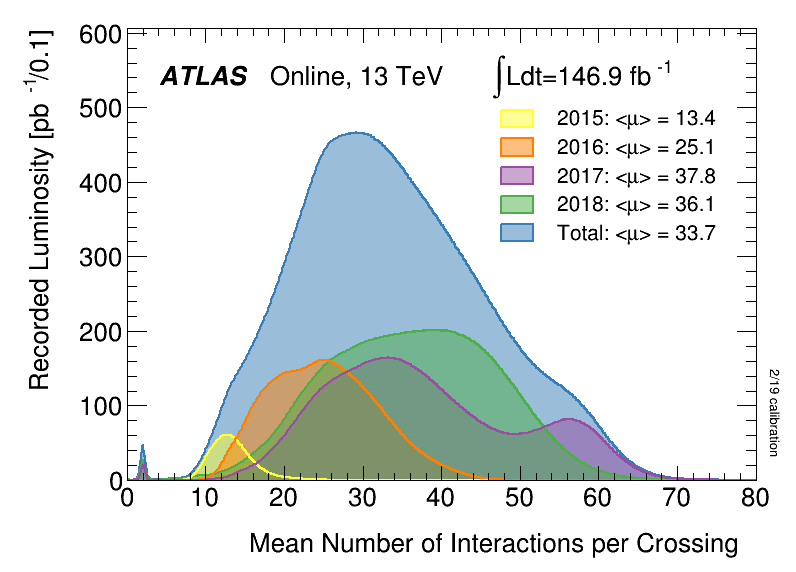
\includegraphics[width=\textwidth,keepaspectratio]{mu_2015_2018.png}
			\caption{ Number of Interactions per bunch crossing in \gls{atlas} Run 2 \cite{run2lumi}. The little bump around $\mu \approx 2$ corresponds to special low pile-up runs.}
			\label{fig::run2lumi}
			\end{figure}
			\begin{table}
			\centering			
			\begin{tabular}{|l|c|c|c|}
			\hline
			\textbf{Collision energy} & \textbf{Year}& \textbf{Integrated luminosity, $pb^{-1}$ }&  Total uncertainty, \%\\
			\hline
			5 TeV  & 2017 & 258& 1.6\\
			13 TeV  & 2017 & 148& 2.1 \\
			13 TeV  & 2018 & 193& 1.5\\
			\hline
			\end{tabular}
			\caption{Energy and luminosity of the special low-mu runs.}
			\label{tab:lowmu}
			\end{table}
\newpage
\chapter{Electromagnetic shower shapes correction in the electromagnetic calorimeter }
    \chapterprecishere{
        ``Potentielle citation sans aucun rapport avec le sujet"\par\raggedleft--- \textup{Personne inconnue}, contexte à déterminer
    }

  \section{Introduction}
  The design and functionality of the ATLAS electromagnetic calorimeter was described in \ref{emc}. Let's consider a bit more in detail the physical processes happening in the \gls{emc}. \\
  It order to measure particle's energy within the calorimeter we must make the particle to loose its entire energy within the calorimeter. For the electrons and photons with energies over few MeV (which is the case for the ATLAS experiment) the primary energy loss mechanism lies in bremsstrahlung radiation and pair creation). The two processes complete each other, so when a high-energy electron or photon gets into the calorimeter, it creates an avalanche-like processus called the electromagnetic shower when a bremsstrahlung-radiated photons create more electron-positron pairs which in turn radiate more bremsstrahlung photons and so on and so forth (see fig. \ref{fig::em_shower}.)\\
  	\begin{figure}[htbp]
  	\begin{subfigure}[t]{0.5\textwidth}
  		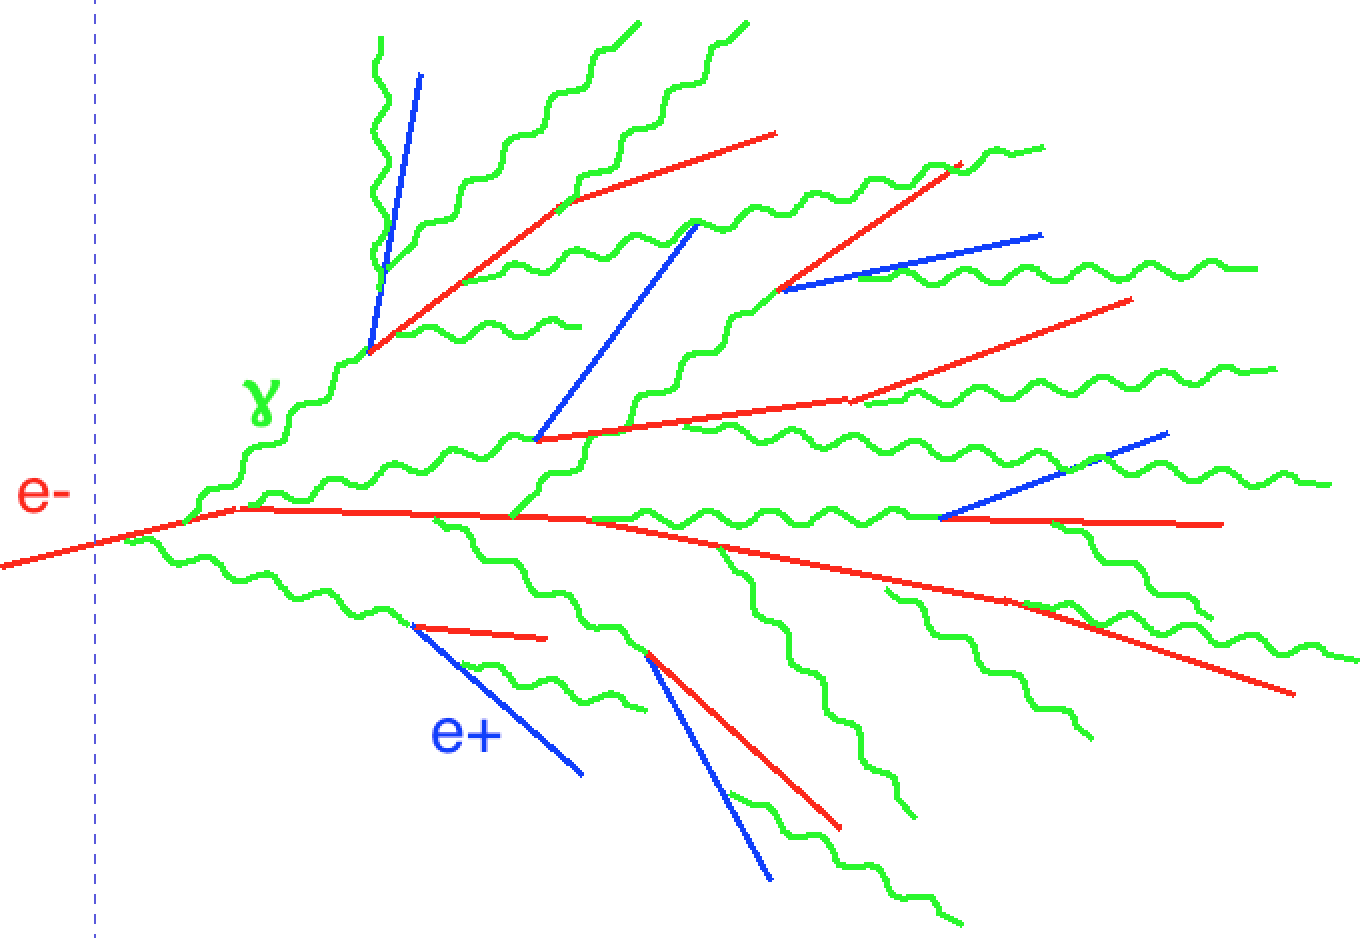
\includegraphics[width=\textwidth,keepaspectratio]{em_shower.png}
  		\caption[Started by an electron]{Initiated by an electron}
  		\label{fig::id}
  	\end{subfigure}
  	\hfill
  	\begin{subfigure}[t]{0.5\textwidth} 
  		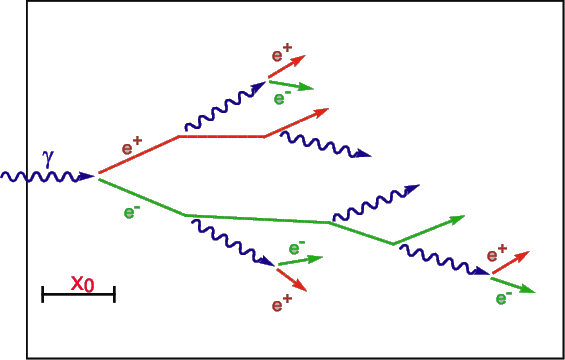
\includegraphics[width=\textwidth,keepaspectratio]{emshower.png}
  		\caption[Started by a $\gamma$-photon]{Initiated by a $\gamma$-photon}
  		\label{fig::pd}
  	\end{subfigure}
  	\caption{The schematic portrayal of EM shower development}
  	\label{fig::em_shower}
  \end{figure}
    The longitudinal and transverse development of the shower depends on the type of the initial particle and on its energy. The energy is well measured by the calorimeter, but identifying the particle still remains a challenging task. The transverse granularity of the ATLAS calorimeter allows to resolve the energy distribution withn the electromagnetic shower in the transverse plane. This information can later be used for particle identification.\\
  When an e/$\gamma$ particle hits the calorimeter its footprint in the second layer of the calorimeter is visible as a cluster of calorimeter cells centered at the central cell having the most energy deposited (sometimes referred to as "the hottest cell"). Roughly 90$\%$ of shower energy is contained in the core 3x3 cells.  We have considered a cluster of 7x11 ($\eta$ x $\phi$) cells, which is schematically depicted on fig. \ref{fig::profile_log}.
  
  
    	\begin{figure}[htbp]
  	\begin{subfigure}[t]{0.5\textwidth}
  		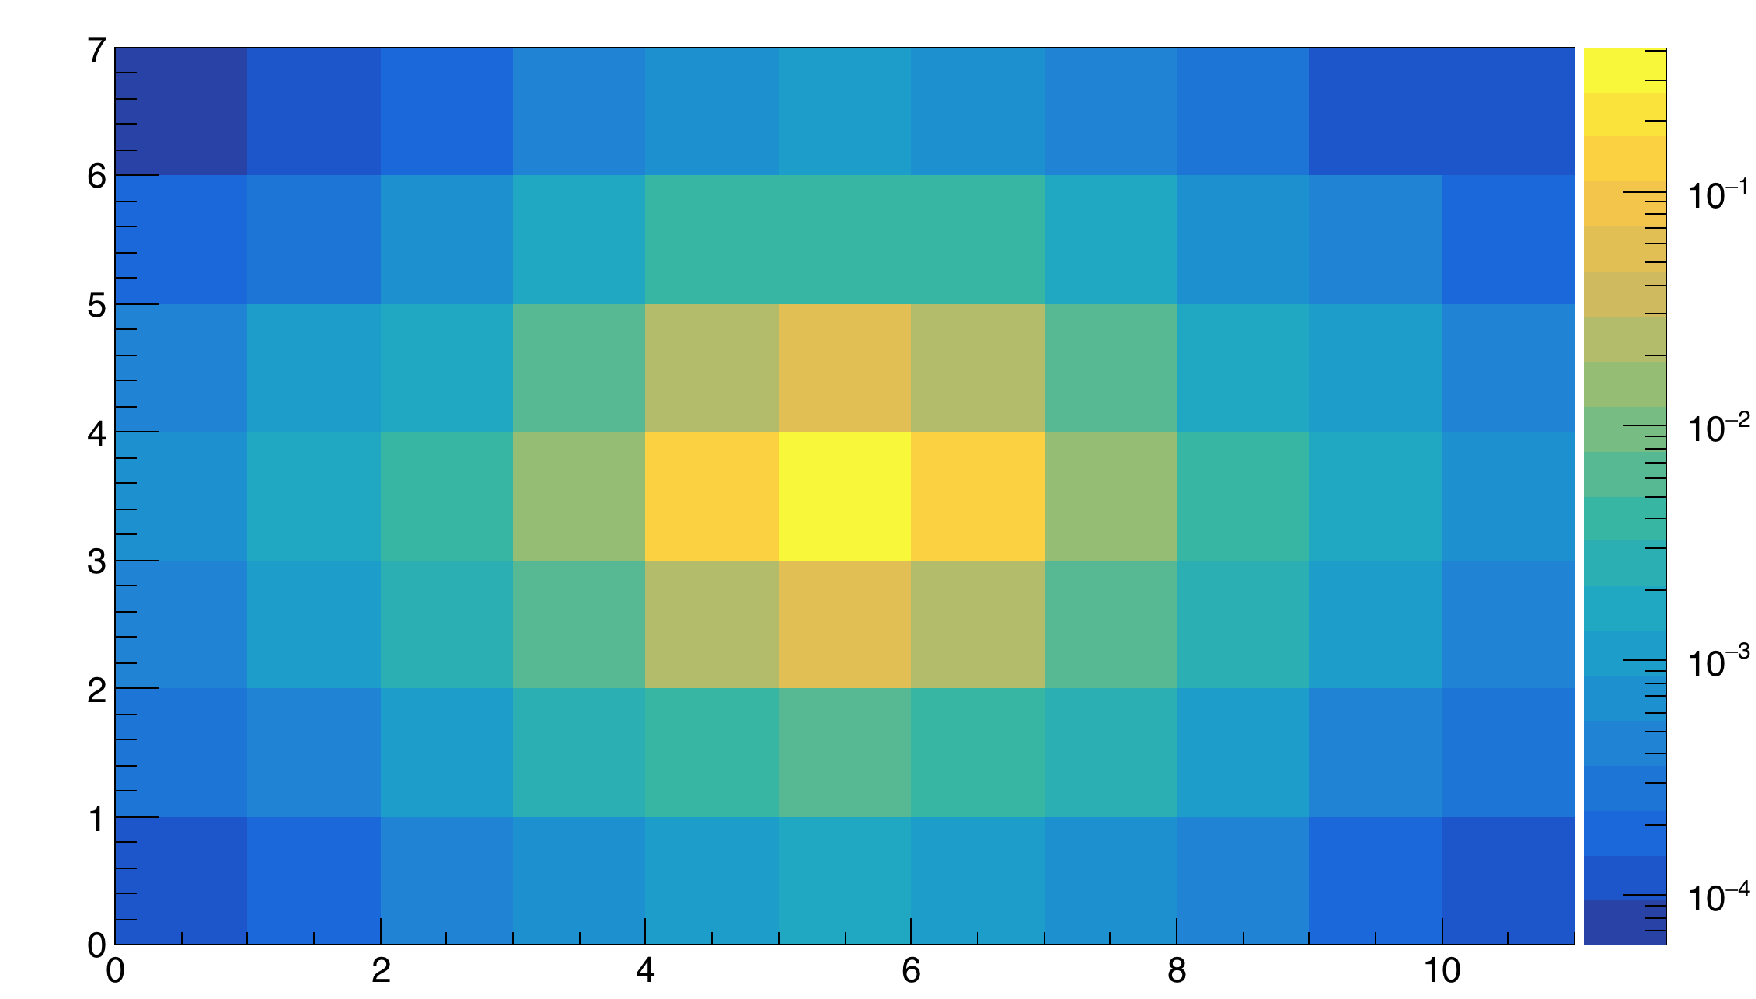
\includegraphics[width=\textwidth,keepaspectratio]{logscale.pdf}
  		\caption{Energy profile of a window of 7x11 cells in the 2nd calorimeter layer (logarithmic scale)}
  		\label{fig::profile_log}
  	\end{subfigure}
  	\hfill
  	\begin{subfigure}[t]{0.5\textwidth} 
  		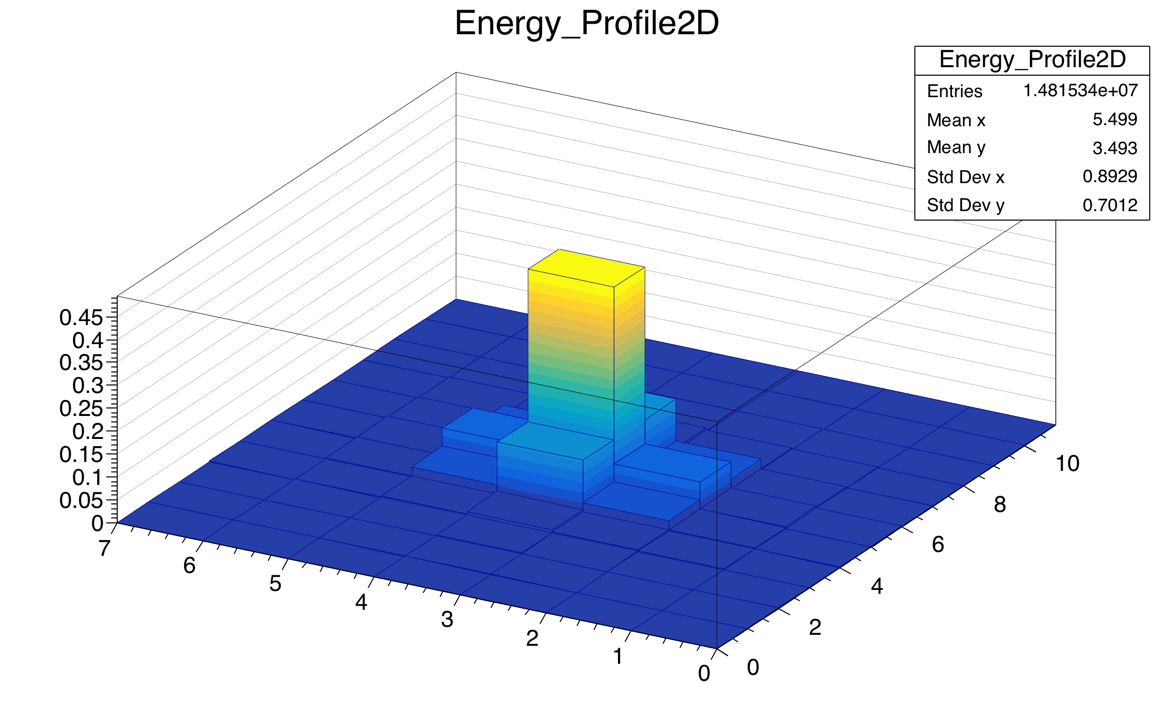
\includegraphics[width=\textwidth,keepaspectratio]{2dProfile.png}
  		\caption{2D profile of the cluster}
  		\label{fig::2d_profile}
  	\end{subfigure}
  	\caption{Visualisations of the 7x11 calorimeter cluster}
  	\label{fig::profiles}
  \end{figure}
  
  In order to characterise the energy distribution within the shower profile a number of observables called shower shapes are used. They are then used as an input for particle identification MVA algorithm. Current study focuses on the second layer of the calorimeter for which there are three shower shape observables described below \cite{egamma_perf_2017}:
  
    	\begin{figure}[htbp]
  	\begin{subfigure}[t]{0.4\textwidth}
  		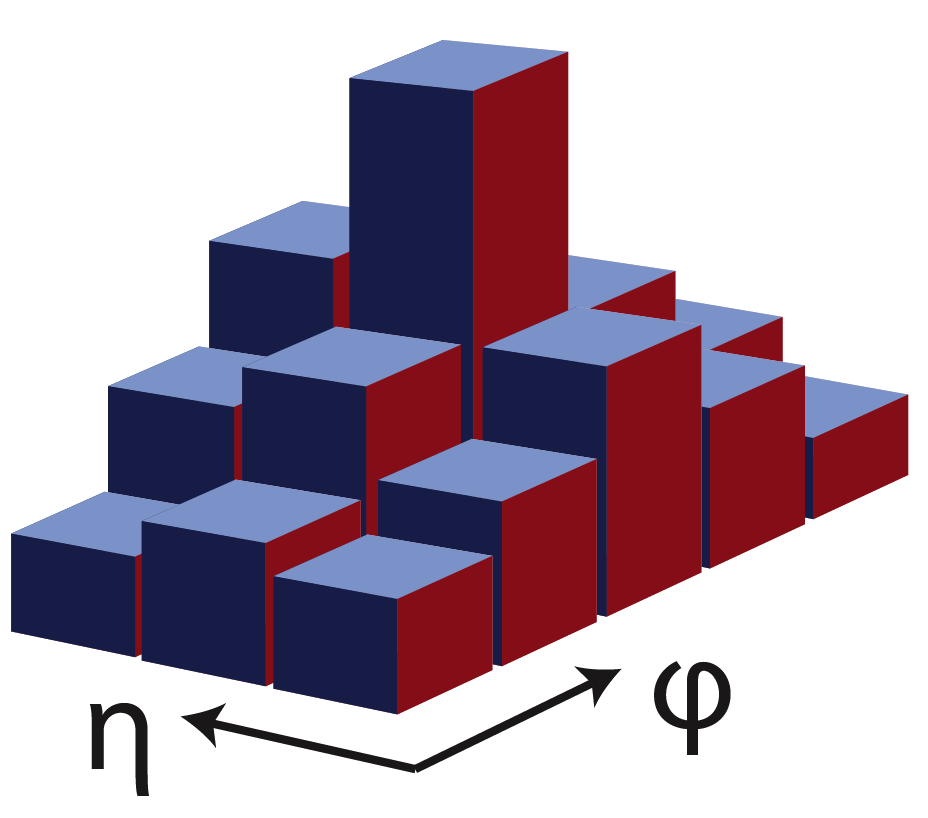
\includegraphics[width=\textwidth,keepaspectratio]{Weta2.png}
  		\caption[Lateral shower width $W_{\eta} 2$]{Lateral shower width $W_{\eta} 2$}
  		\label{fig::weta2}
  	\end{subfigure}
  	\hfill
  	\begin{subfigure}[t]{0.25\textwidth} 
  		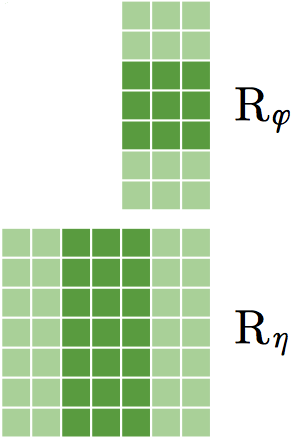
\includegraphics[width=\textwidth,keepaspectratio]{reta_rphi.png}
  		\caption[$R_{\phi}$ and $R_{\eta}$]{$R_{\phi}$ and $R_{\eta}$}
  		\label{fig::reta_rphi}
  	\end{subfigure}
  	\caption{Shower shapes in the second layer of the electromagnetic calorimeter}
  	\label{fig::sshapes}
  \end{figure}
  
  \begin{itemize}
  	\item Lateral shower width $W_{\eta 2} = \sqrt{\sum(E_i \eta^{2}_{i})-(\sum(E_i \eta_{i})/\sum(E_i))^2}$ calculated within a window of 3x5 cells.
  	\item $R_{\phi}$ - ratio of the energy in 3x3 cells over the energy in 3x7 cells centered around the hottest cell.
  	\item $R_{\eta}$ - ratio of the energy in 3x7 cells over the energy in 7x7 cells centered around the hottest cell.
  \end{itemize}
  
  The shower shapes distributions for different types of particles is shown in fig. \ref{sshapes_simul} - although the distributions overlap, combining the shower shapes information with the inputs from other detectors allow to identify the particle.  
    	\begin{figure}[htbp]
	\begin{subfigure}[t]{0.4\textwidth}
		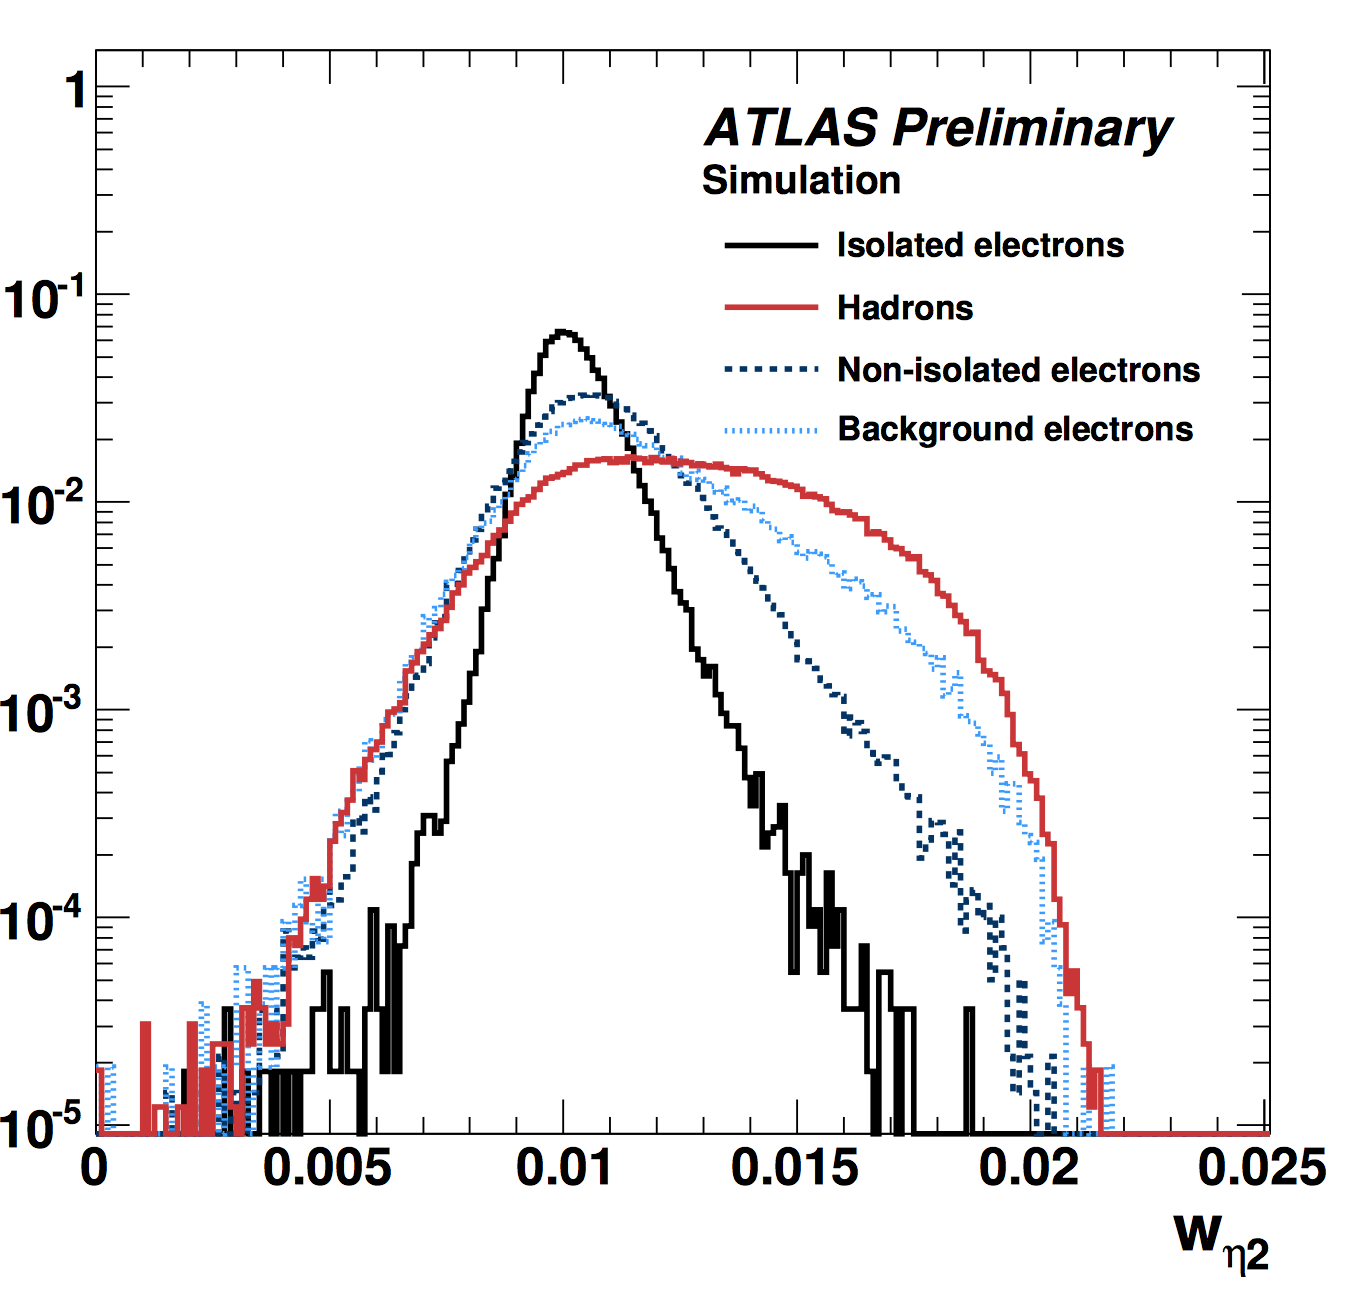
\includegraphics[width=\textwidth,keepaspectratio]{Weta2Simulation.png}
		\caption[ $W_{\eta 2}$]{$W_{\eta 2}$ distribution simulation}
		\label{fig::weta2_simul}
	\end{subfigure}
	\hfill
	\begin{subfigure}[t]{0.39\textwidth} 
		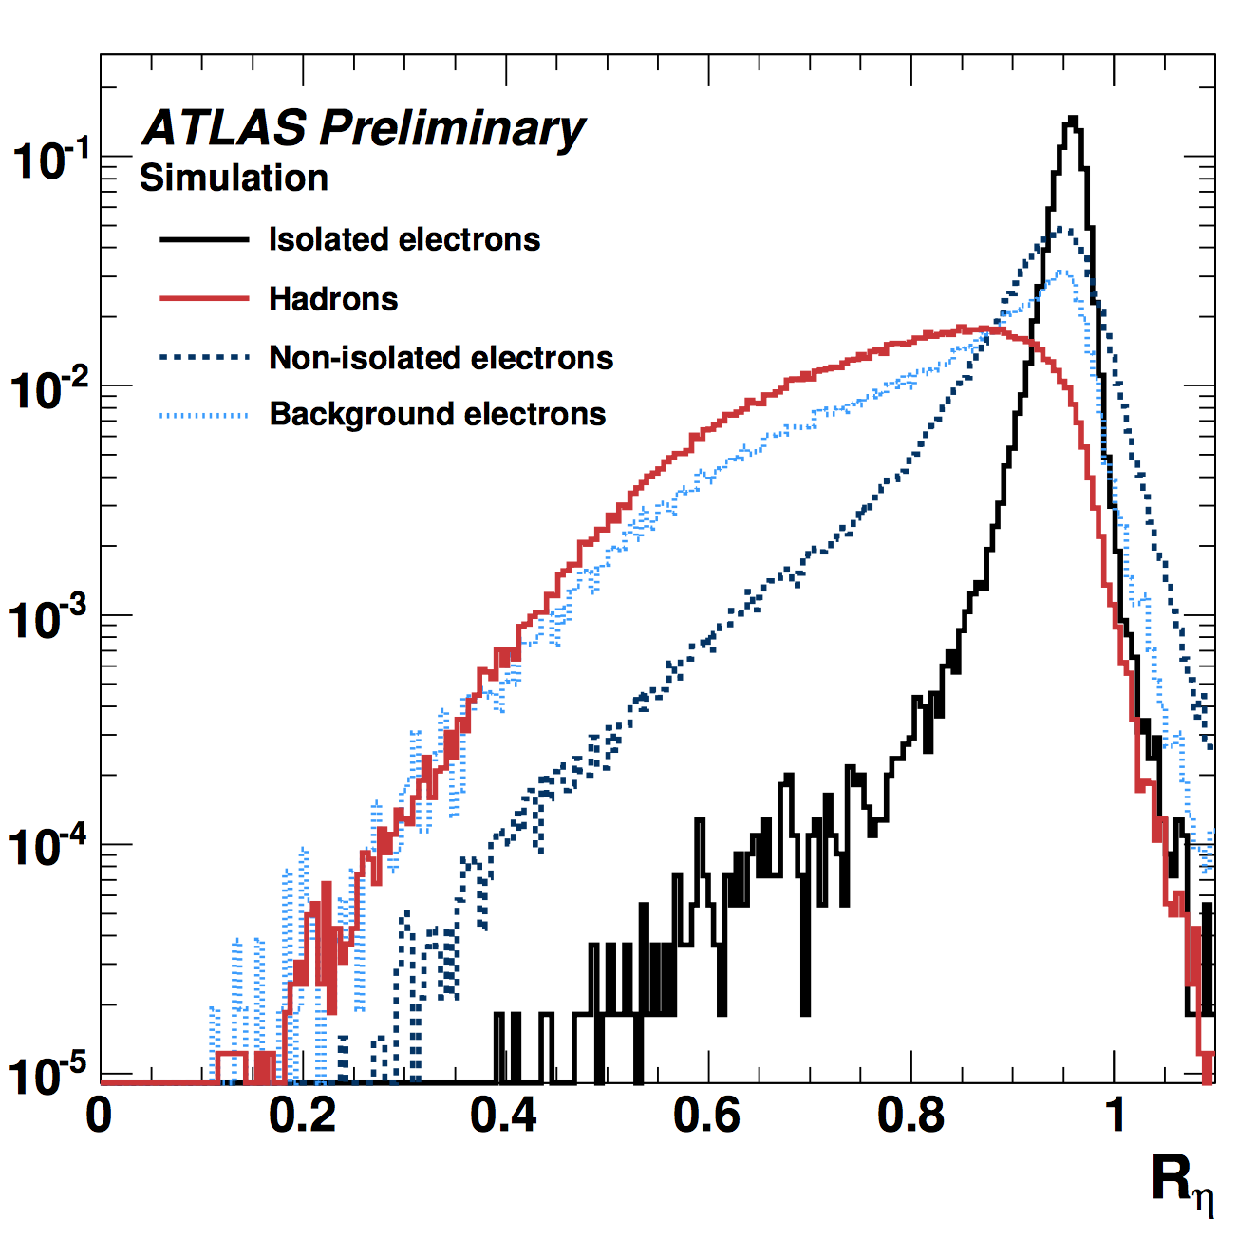
\includegraphics[width=\textwidth,keepaspectratio]{RetaSimulation.pdf}
		\caption[ $R_{\eta}$]{$R_{\eta}$ distribution simulation}
		\label{fig::reta_simul}
	\end{subfigure}
  	\caption{Distribution of $R_{\eta}$ in simulation (GEANT4) for electrons and jets \cite{sshapes_simulation}.}
	\label{fig::sshapes_simul}
\end{figure}

  Figure \ref{reta_simul} shows how $R_{\eta}$ distribution is different in jets, signal electrons and background electrons. Background electrons denote non-prompt electrons which are not originated from primary vertex. \\
 
   The shower shapes appear to be extremely sensitive to the detector material modelling. A simplification in the geometry of the EMCal absorber geometry in GEANT4 9.2 (a layered structure of the accordion was represented as a homogenous material) has lead to visible discrepancies in the shower shapes between the data and MC. This was corrected in GEANT4 9.4 significantly improving the agreement, although not eliminating it completely (see fig. \ref{fig::sshapes_geant}).  The origin for the remaining discrepancy is not clear.\\
      	\begin{figure}[htbp]
  	\begin{subfigure}[t]{0.4\textwidth}
  		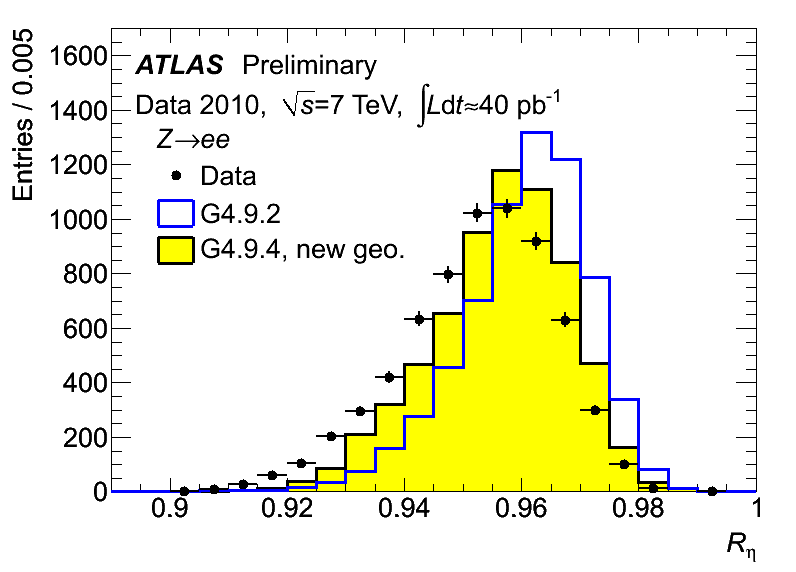
\includegraphics[width=\textwidth,keepaspectratio]{Reta_G}
  		\caption[ $W_{\eta 2}$]{$W_{\eta 2}$}
  		\label{fig::weta2_geant}
  	\end{subfigure}
  	\hfill
  	\begin{subfigure}[t]{0.4\textwidth} 
  		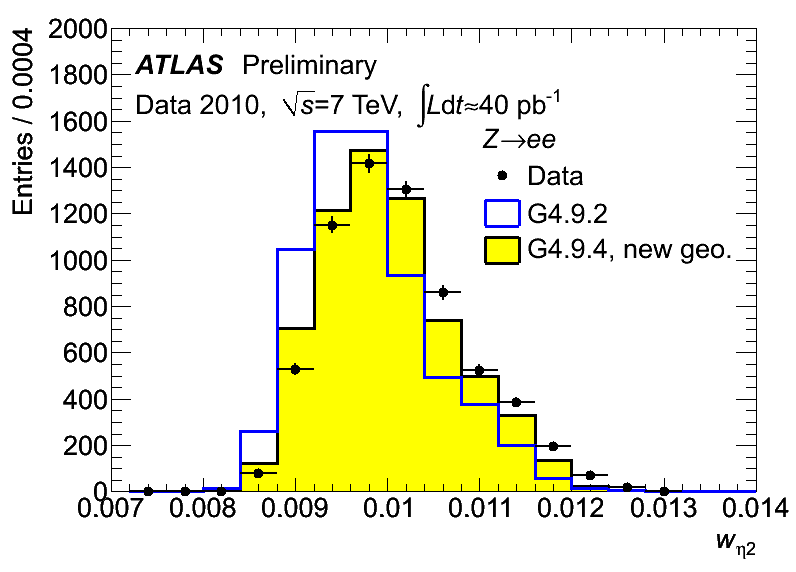
\includegraphics[width=\textwidth,keepaspectratio]{weta2_G}
  		\caption[ $R_{\eta}$]{$R_{\eta}$ }
  		\label{fig::reta_geant}
  	\end{subfigure}
  	\caption{Data/MC Comparison for Calorimeter Shower Shapes of High Et Electrons \cite{geant_corr}.}
  	\label{fig::sshapes_geant}
  \end{figure}
  
  Disagreement in shower shapes between the data and MC leads to discrepancies in particle ID which are later fixed using $\eta-$ and $p_T$-dependent scale factors. Correction of the shower shapes aims to get the scale factors closer to unity, reducing the corresponding systematic uncertainties and improving the precision of the measurements with electrons in the final states.  

  
  \section{ Shower shapes measurement and correction  }
  \subsection{Event selection}
  For this study we have considered electrons from the $Z\rightarrow ee$ decay. A set of recommended single electron triggers was used (HLT\_e26\_lhtight\_nod0\_ivarloose, HLT\_e60\_lhmedium\_nod0,\\
   HLT\_e140\_lhloose\_nod0,HLT\_e300\_etcut). Each event was required to have 2 electrons at least one of which has $p_T>25$ GeV.  In order to suppress the background both electrons had to pass gradient isolation. Z invariant mass cut was applied with a window of $80-120$GeV. To avoid identification bias from triggering the tag and probe approach was used with only probe electrons taken into consideration \cite{RecoID2011}. The electron cluster in the second calorimeter layer was required to contain information from 77 calorimeter cells. No pile-up reweighting has been applied. Datasets of 264786295 events in data (2017 proton-proton collisions) and 79340000 events in MC (Powheg+Pythia8) were used. 
  \subsection{Data/MC discrepancies}
  Our consideration begins with the energy deposit of an electron in the second layer of the calorimeter. A window of 7 cells in $\eta$ and 11 cells in $\phi$ is centered around the cell with the highest energy.

  Shower shapes were considered in 14 $\eta$ bins in the range between $|\eta| = (0,2.4)$ in order to investigate how the discrepancy depends on $\eta$. 
    	\begin{figure}[htbp]
  	\begin{subfigure}[t]{0.5\textwidth}
  		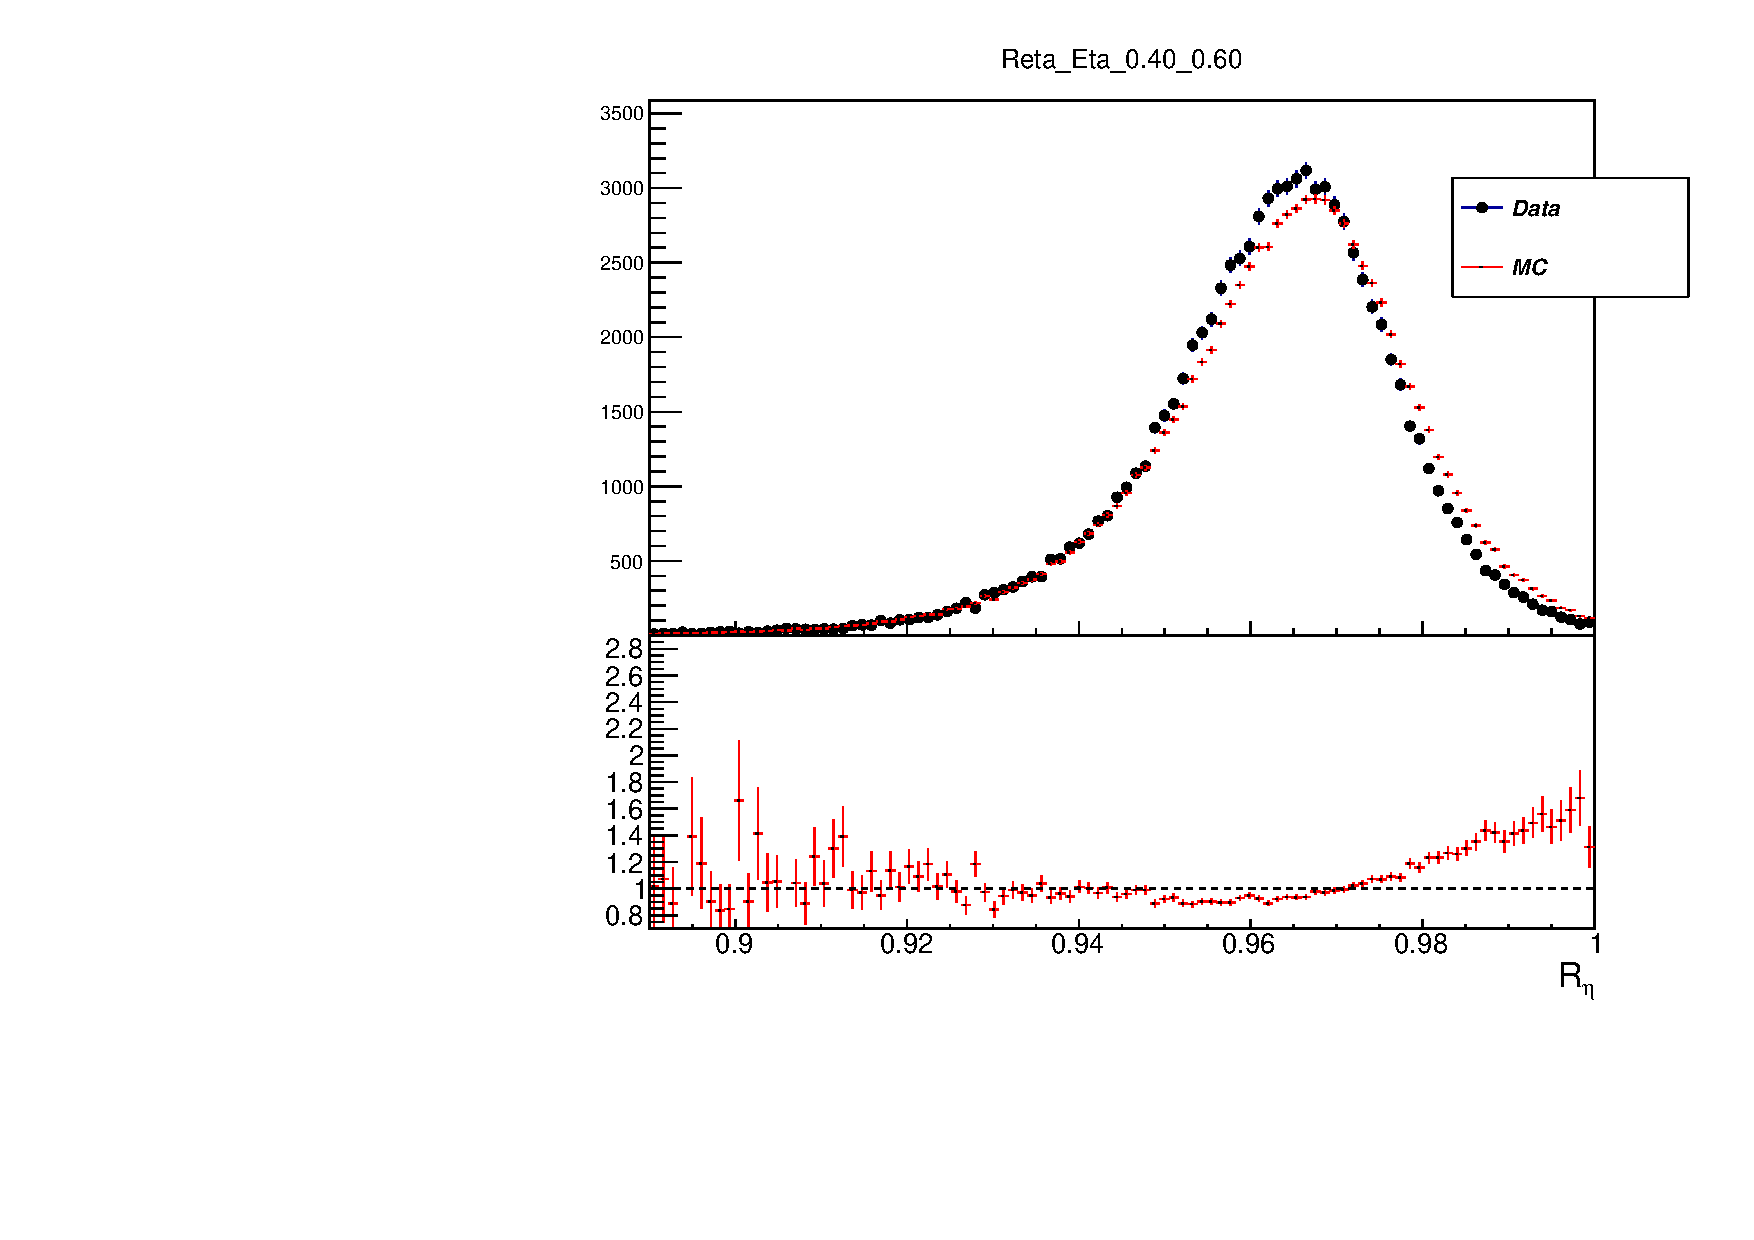
\includegraphics[width=\textwidth,keepaspectratio]{Reta2_Eta_4_6.pdf}
  		\caption{$R_{\eta}$ in $|\eta| = (0.4,0.6)$ }
  		\label{fig::reta_norew_04}
  	\end{subfigure}
  	\hfill
  	\begin{subfigure}[t]{0.5\textwidth} 
  		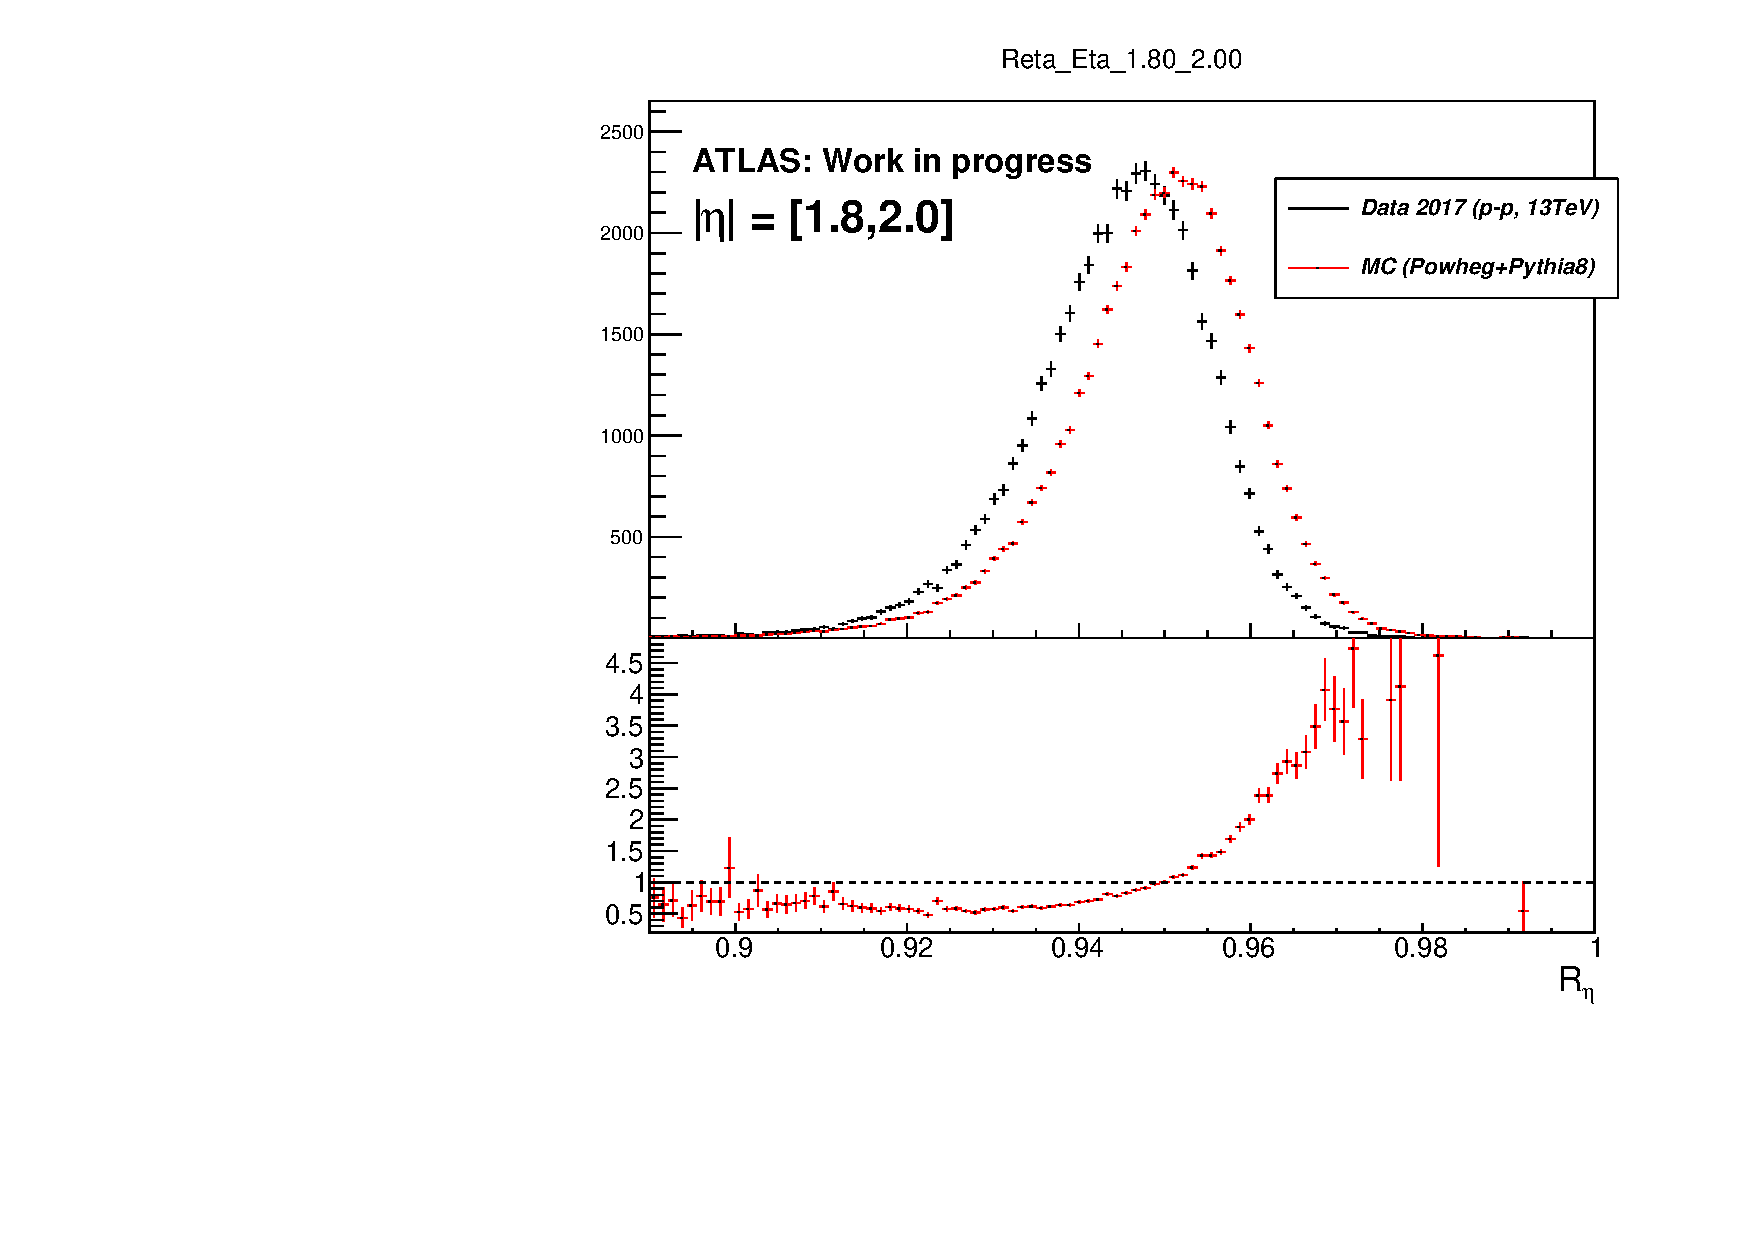
\includegraphics[width=\textwidth,keepaspectratio]{Reta2_Eta_18_20.pdf}
  		\caption{$R_{\eta}$ in $|\eta| = (1.8,2.0)$ }
  		\label{fig::reta_norew_18}
  	\end{subfigure}
  	\caption{$R_{\eta}$ in the barel and in the end-cap, Data vs MC}
  	\label{fig::reta_norew}
  \end{figure}

    \begin{figure}[htbp]
	\begin{subfigure}[t]{0.5\textwidth}
		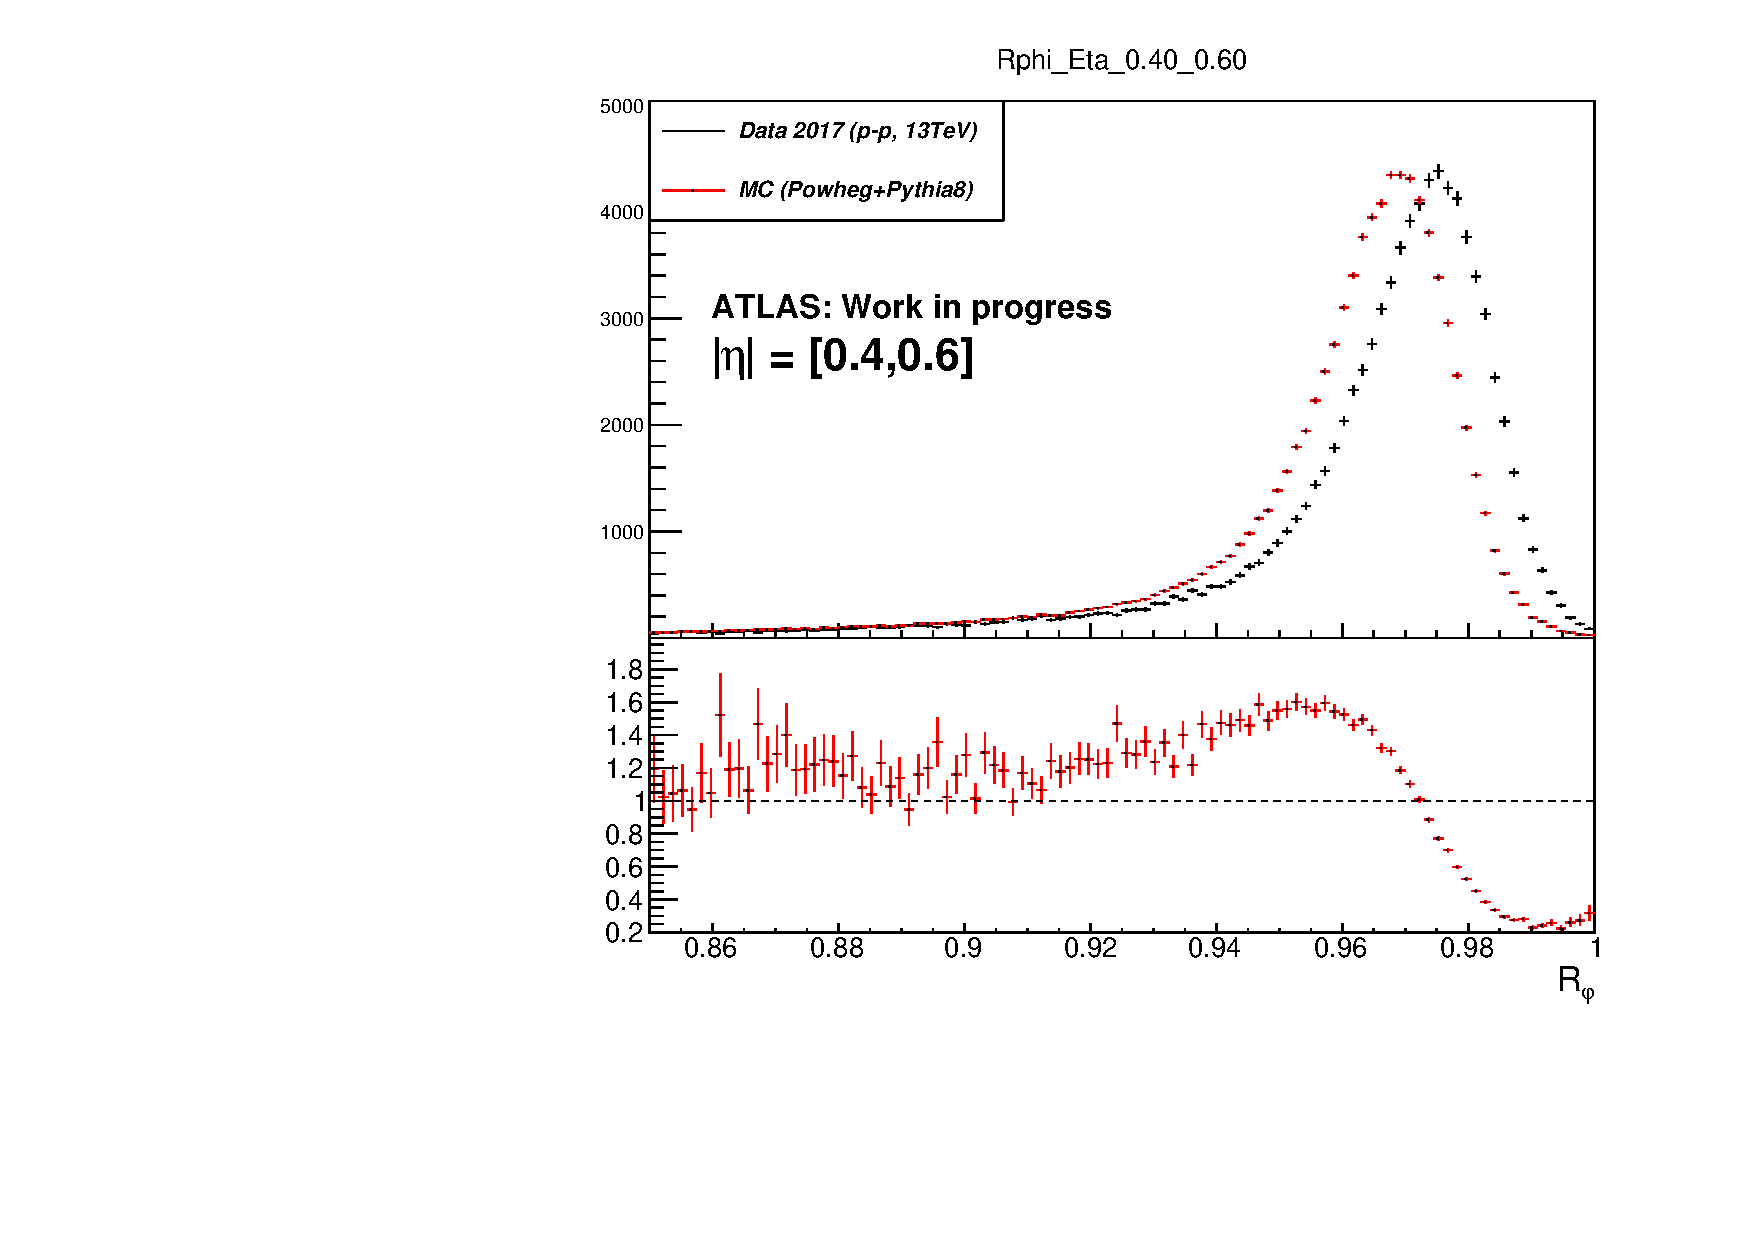
\includegraphics[width=\textwidth,keepaspectratio]{Rphi2_Eta_4_6.pdf}
		\caption{$R_{\phi}$ in $|\eta| = (0.4,0.6)$ }
		\label{fig::rphi_norew_04}
	\end{subfigure}
	\hfill
	\begin{subfigure}[t]{0.5\textwidth} 
		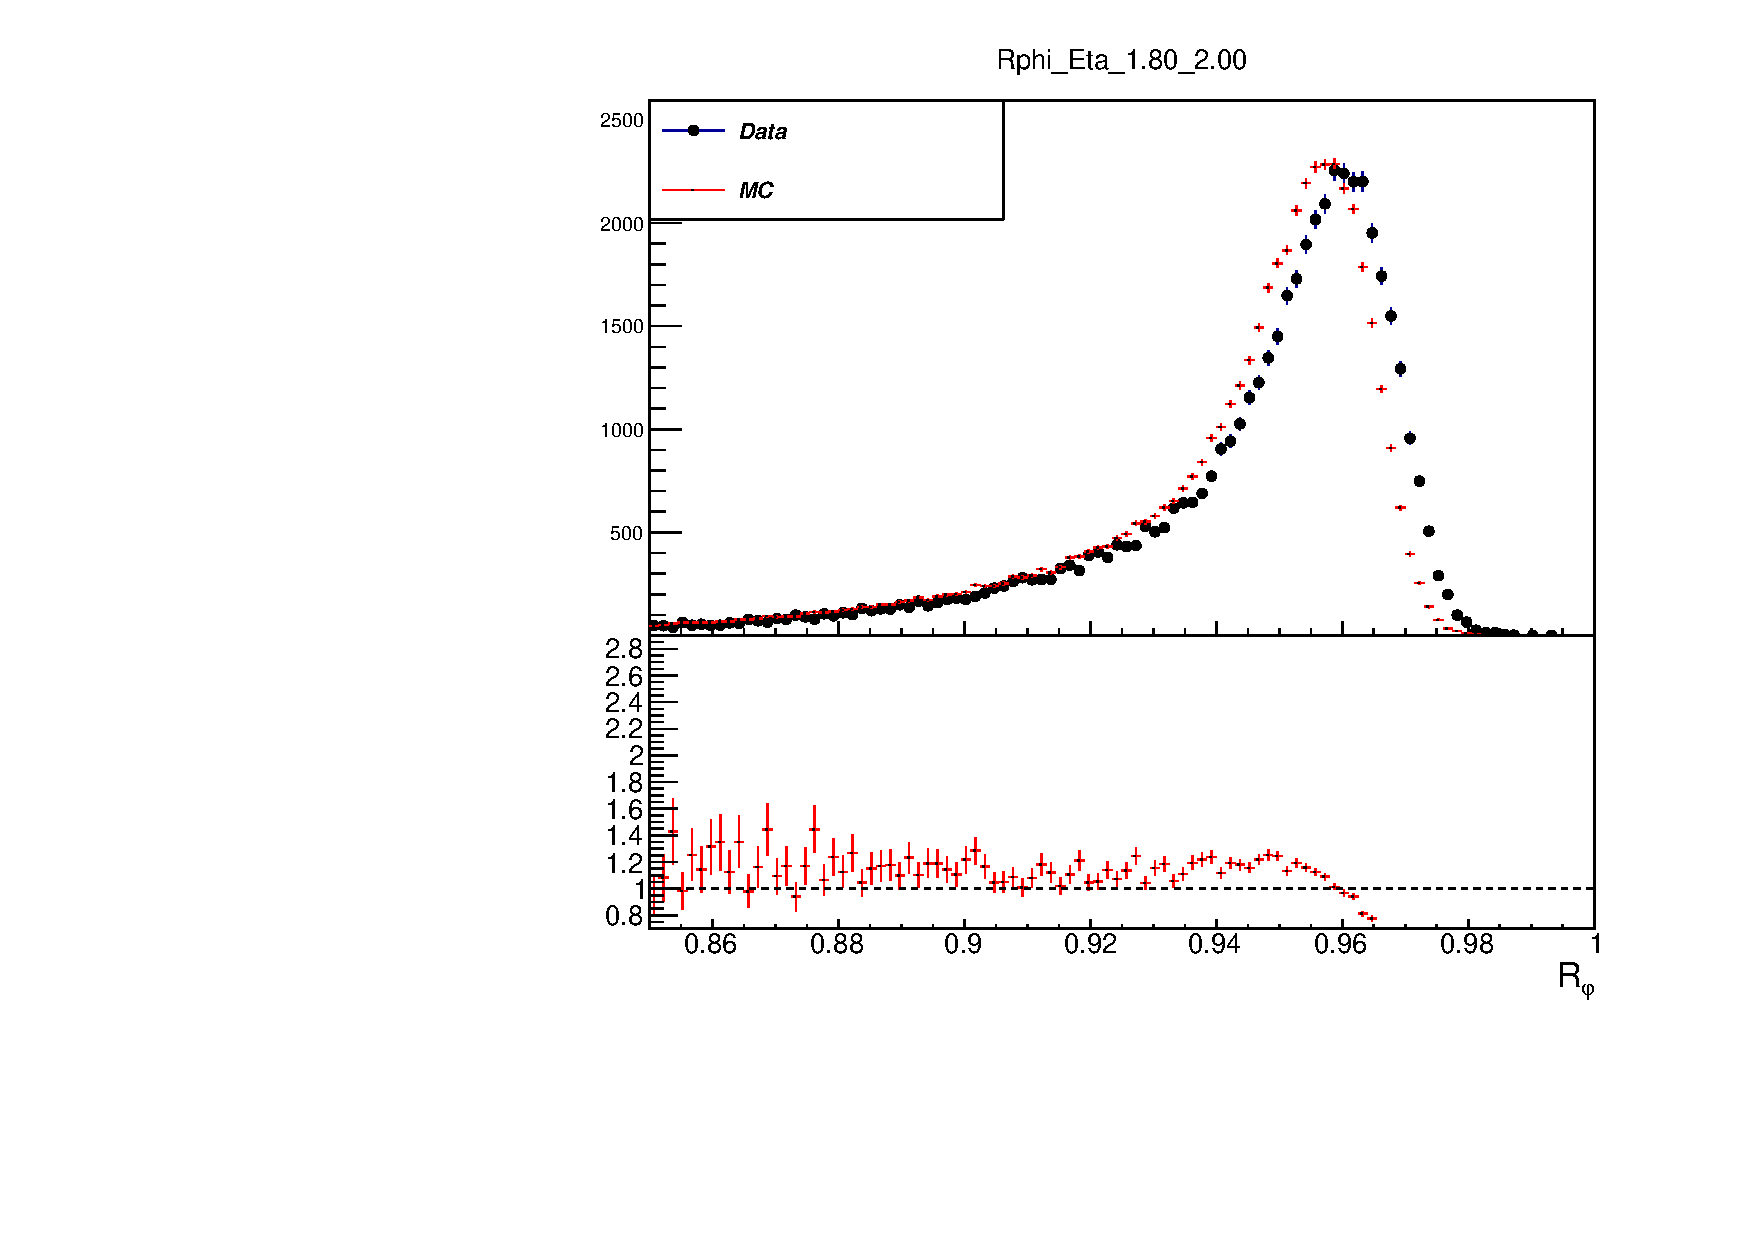
\includegraphics[width=\textwidth,keepaspectratio]{Rphi2_Eta_18_20.pdf}
		\caption{$R_{\phi}$ in $|\eta| = (1.8,2.0)$ }
		\label{fig::rphi_norew_18}
	\end{subfigure}
	\caption{$R_{\phi}$ in the barel and in the end-cap, Data vs MC}
	\label{fig::rphi_norew}
\end{figure}
  
    \begin{figure}[htbp]
	\begin{subfigure}[t]{0.5\textwidth}
		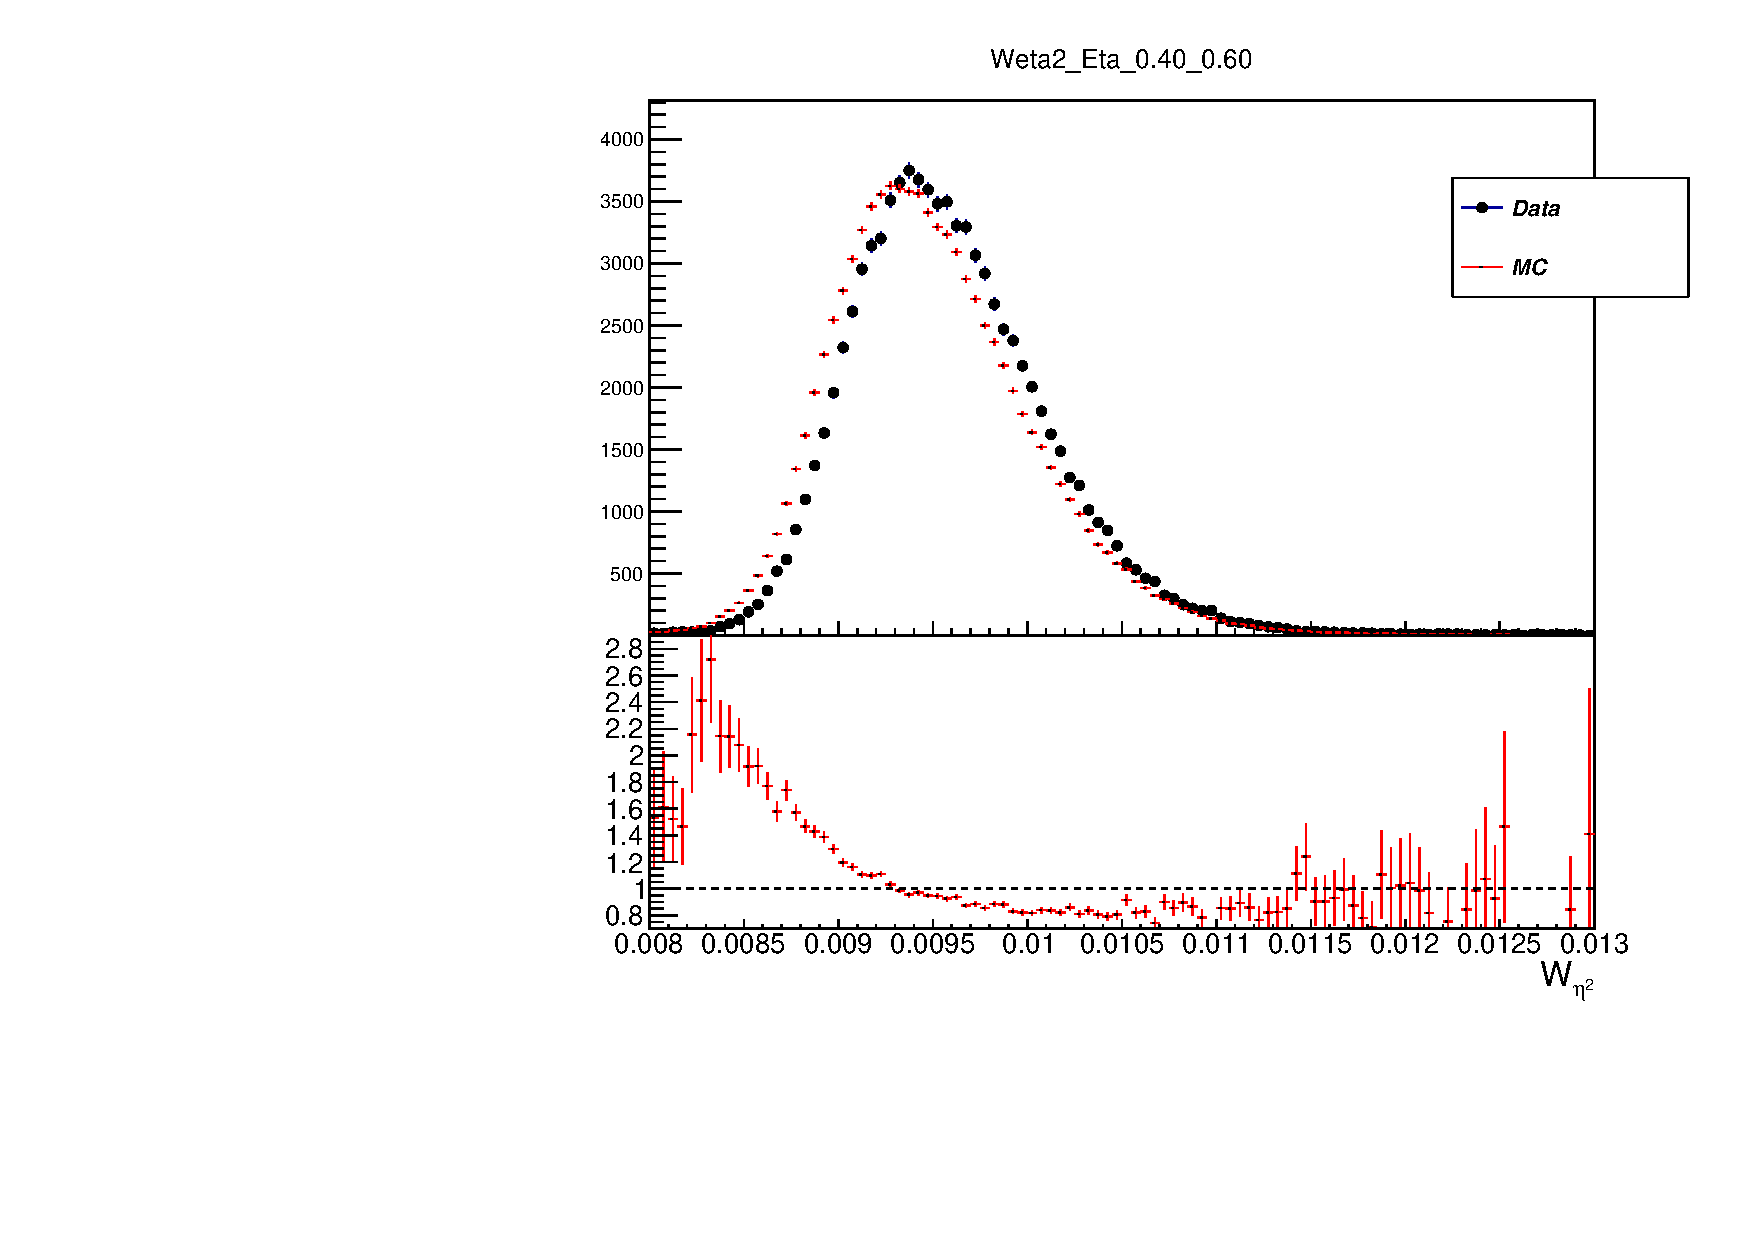
\includegraphics[width=\textwidth,keepaspectratio]{weta22_Eta_4_6.pdf}
		\caption{$W_{\eta}^2$ in $|\eta| = (0.4,0.6)$ }
		\label{fig::weta2_norew_04}
	\end{subfigure}
	\hfill
	\begin{subfigure}[t]{0.5\textwidth} 
		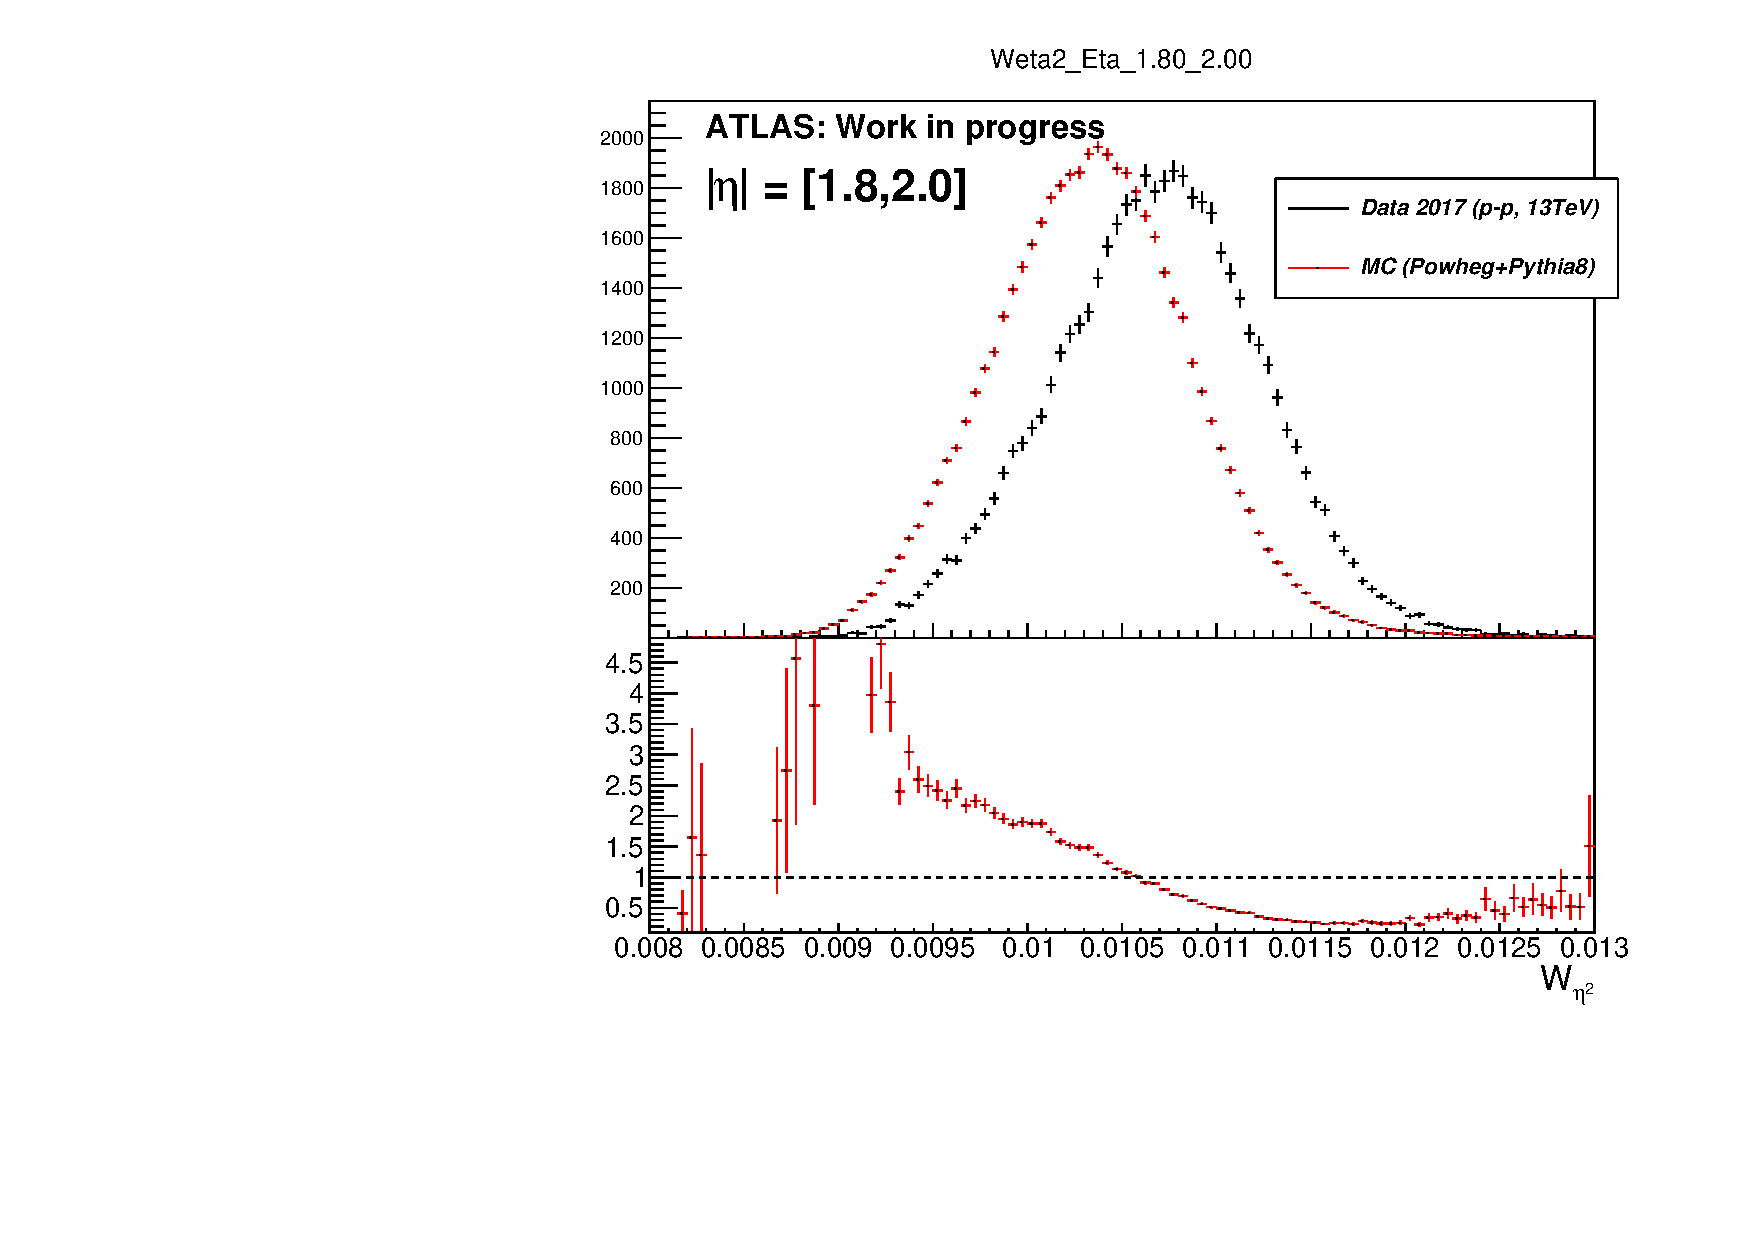
\includegraphics[width=\textwidth,keepaspectratio]{weta22_Eta_18_20.pdf}
		\caption{$W_{\eta}^2$ in $|\eta| = (1.8,2.0)$ }
		\label{fig::weta2_norew_18}
	\end{subfigure}
	\caption{$W_{\eta}^2$ in the barel and in the end-cap, Data vs MC}
	\label{fig::weta2_norew}
\end{figure}



  The $\eta$-dependent shower shapes in data are wider than the MC and show a larger discrepancy in the endcap ($|\eta| = (1.52,2.4)$). For $\phi$ dimension the situation is the opposite: MC is wider than the data and the barrel ($|\eta| = (0,1.52)$) shows larger discrepancy. Figures \ref{Reta2}, \ref{Rphi2}, \ref{Weta22} contain examples of shower shapes in different eta bins. 
  \subsection{The correction procedure}
  \subsubsection{The correction matrix}
  The correction procedure is based on the redistribution of energy between the cluster cells in MC so that the distribution becomes consistent with the data. For every $\eta$ bin a correction matrix is derived in the following way:
  \begin{equation}
  \nonumber
  \large {M_{i}^{Correction} = \frac{E_{i}^{Data}}{\Sigma E^{Data}} - \frac{E_{i}^{MC}}{\Sigma E^{MC}}}
  \end{equation}
  $\Sigma_i M_i^{Correction} = 0$, $i = 1..77$.\\
  $E_i^{Data}$, $E_i^{MC}$ - matrix elements of the averaged energy profiles. 
  The correction is then applied to the electron cluster cells on event-by-event basis:
  \begin{equation}
  \nonumber
  \large {E_{i}^{Reweighted} = {E_{i}^{Non-reweighted}(1+M_{i}^{Correction}).}}
  \end{equation}
  This redistributes the energy among the cells keeping the total energy exactly the same.
  \subsubsection{Bremsstrahlung tails}
  The magnetic field directed along the $\phi$ dimension leads to a significant asymmetry in energy deposits for electrons and positrons (figure \ref{chargeAsym}). 
  
  
      \begin{figure}[htbp]
  	\begin{subfigure}[t]{0.5\textwidth}
  		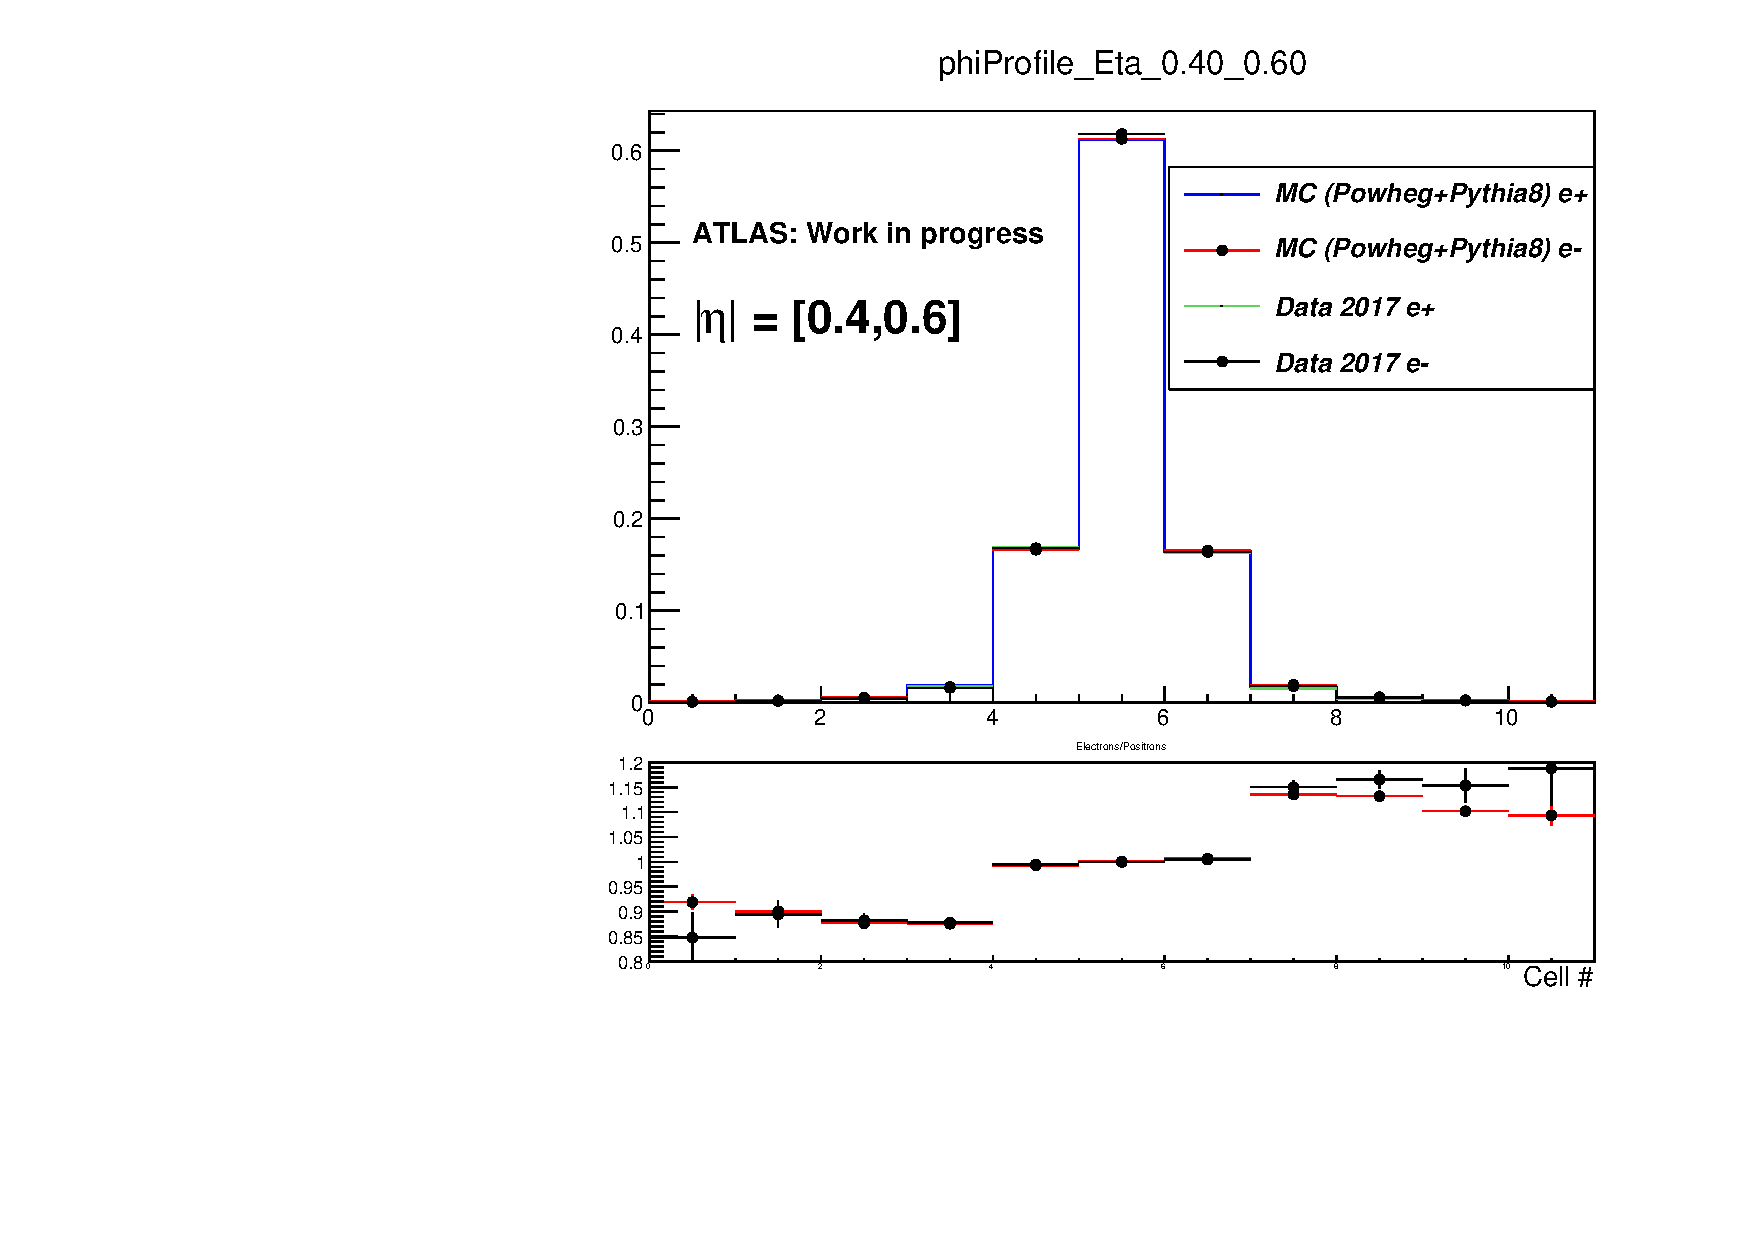
\includegraphics[width=\textwidth,keepaspectratio]{phiProfileDataMC_Eta_4_6.pdf}
  		\caption{$R_{\phi}$ in $|\eta| = (0.4,0.6)$ }
  		\label{fig::rphi_norew_04}
  	\end{subfigure}
  	\hfill
  	\begin{subfigure}[t]{0.5\textwidth} 
  		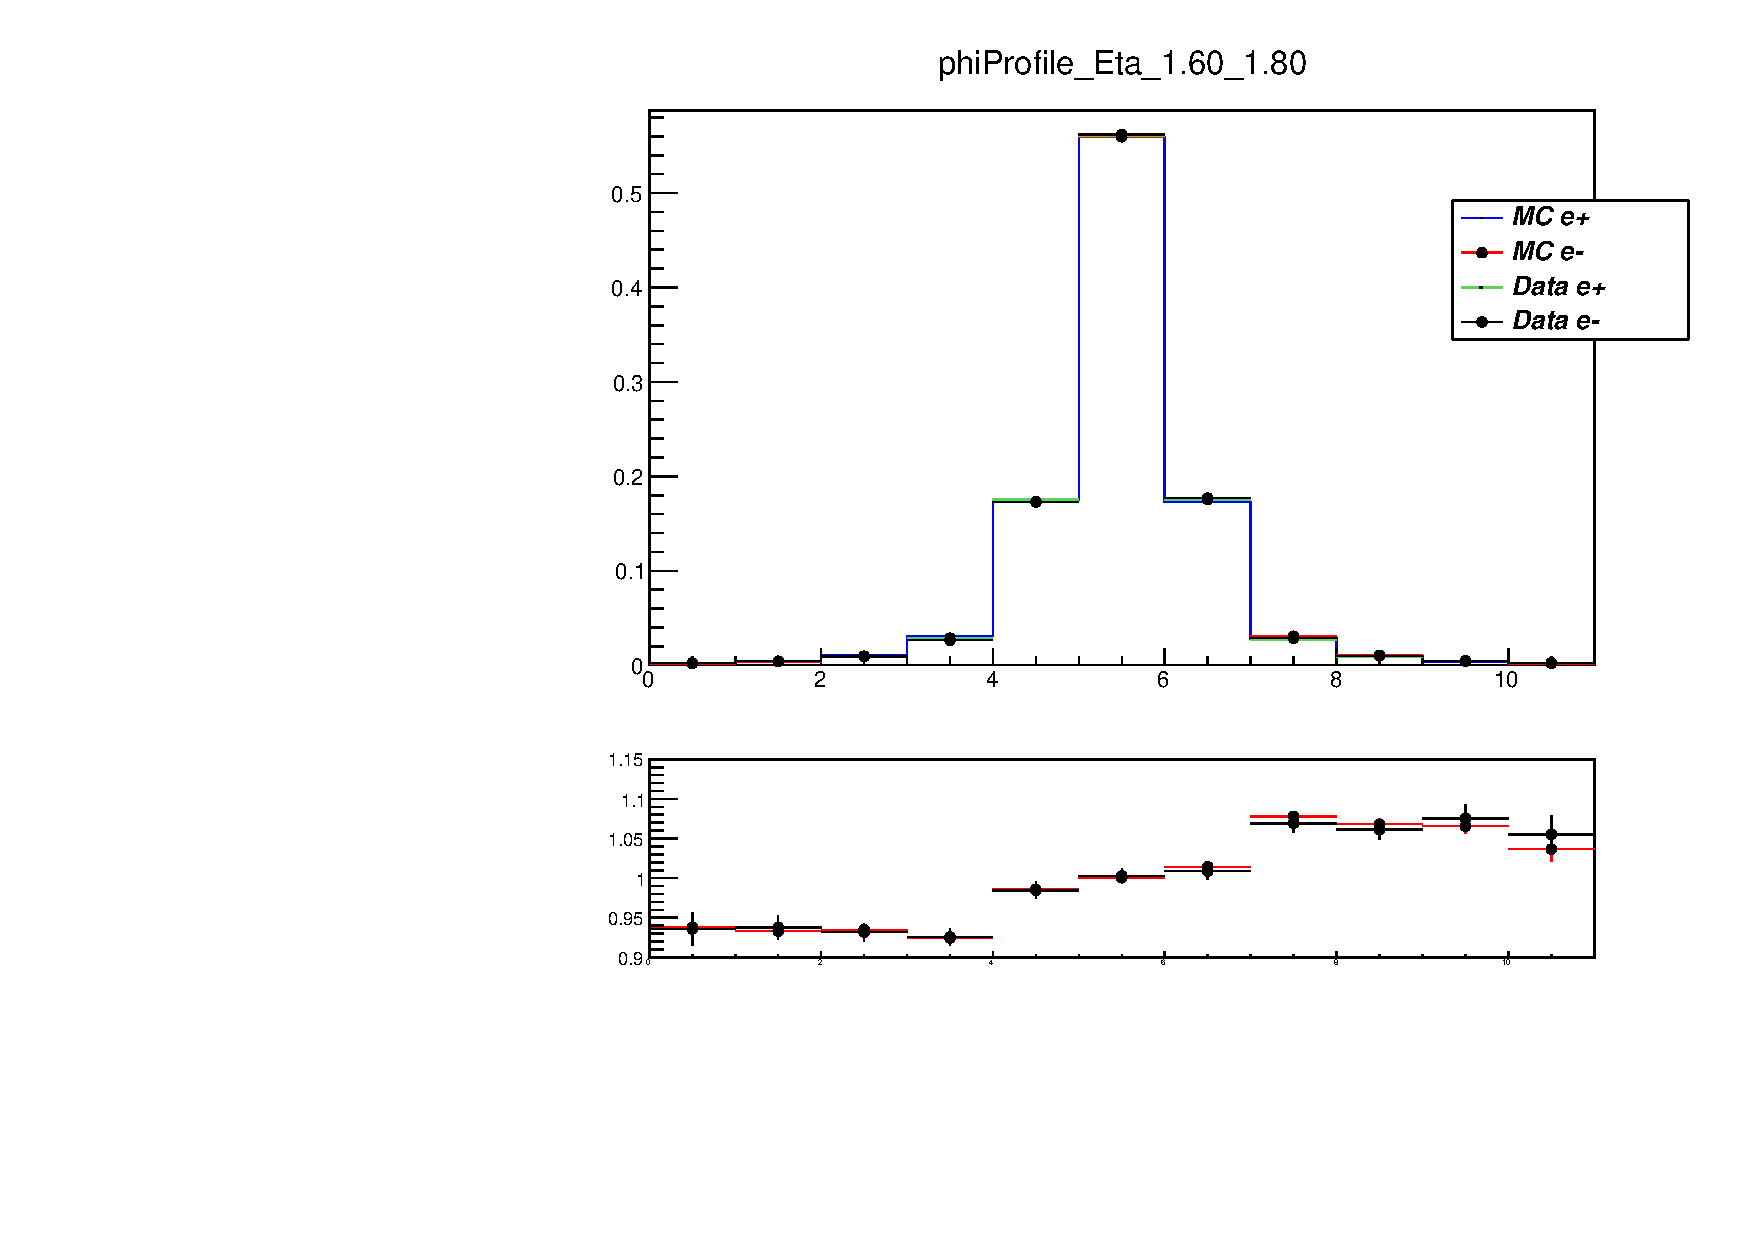
\includegraphics[width=\textwidth,keepaspectratio]{phiProfileDataMC_Eta_16_18.pdf}
  		\caption{$R_{\phi}$ in $|\eta| = (1.8,2.0)$ }
  		\label{fig::rphi_norew_18}
  	\end{subfigure}
  	\caption{$R_{\phi}$ in the barel and in the end-cap, Data vs MC}
  	\label{fig::rphi_norew}
  \end{figure}

  
  Considering the fact that the reweighting is intended to correct for the data/MC discrepancies themselves and not for the bremsstrahlung effect it makes sense to develop the bremsstrahlung-free correction function based on $e^+$ and $e^-$ correction matrices. The principle is schematically explained on figure \ref{bstails}.\\
  \begin{figure}[htbp]
  	\begin{center}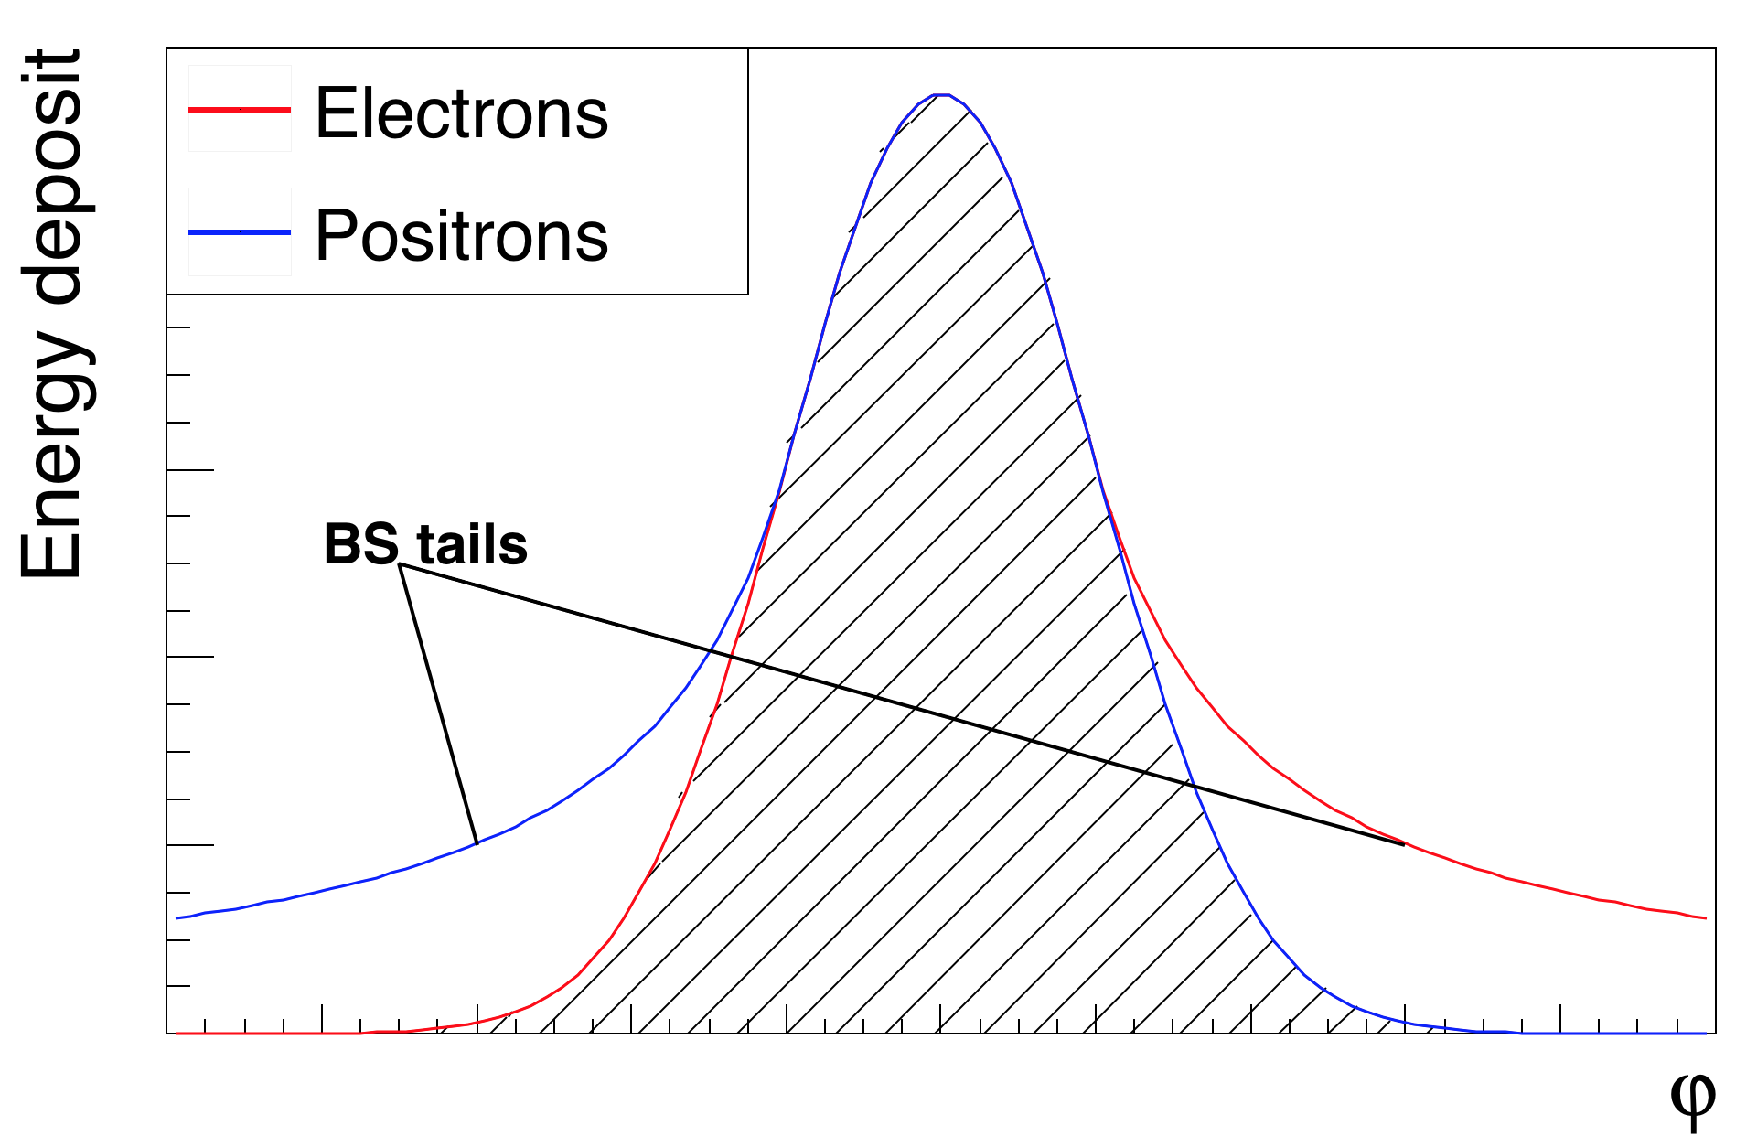
\includegraphics[%
  		width=7cm,
  		keepaspectratio]{bs_tails.pdf}\end{center}
  	\caption{Schematic energy profile in $\phi$ dimension. Bremsstrahlung tails subtraction based on $e^+$ and $e^-$ energy profiles.}
  	\label{bstails}
  \end{figure}
  Good agreement of data and MC description of $e^+$ and $e^-$ asymmetry gives a hint that the material mismodelling cannot be the main source of the data/MC disagreement.\\
  
  \section{Results}
  Figures \ref{fig::reta}, \ref{fig::rphi_rew}, \ref{fig::weta2_rew} show the effect of the correction. The shower shapes in MC become very close to the data, correcting a significant discrepancy. \\
  Figures \ref{fig::integrated} contain shower shapes vs $p_T$ integrated over $\eta$. They demonstrate that the correction does not depend on the $p_T$ which allows to expect the decreased systematic uncertainties for $p_T$ regions distant from $40-50$GeV.\\
  Finally, figure \ref{SF} shows the effect of the correction on electron ID efficiency. We can see a visible improvement, notably in the endcap region.
  Nevertheless the barrel region shows little improvement. It can be explained by the fact that electron ID MVA relies on many variables while only a number of them were corrected during current study.\\
  The proposed method is getting integrated into ATLAS Athena framework as an option and is planned to be used as a baseline for Run 3. 
  
  	\begin{figure}[htbp]
  	\begin{subfigure}[t]{0.5\textwidth}
  		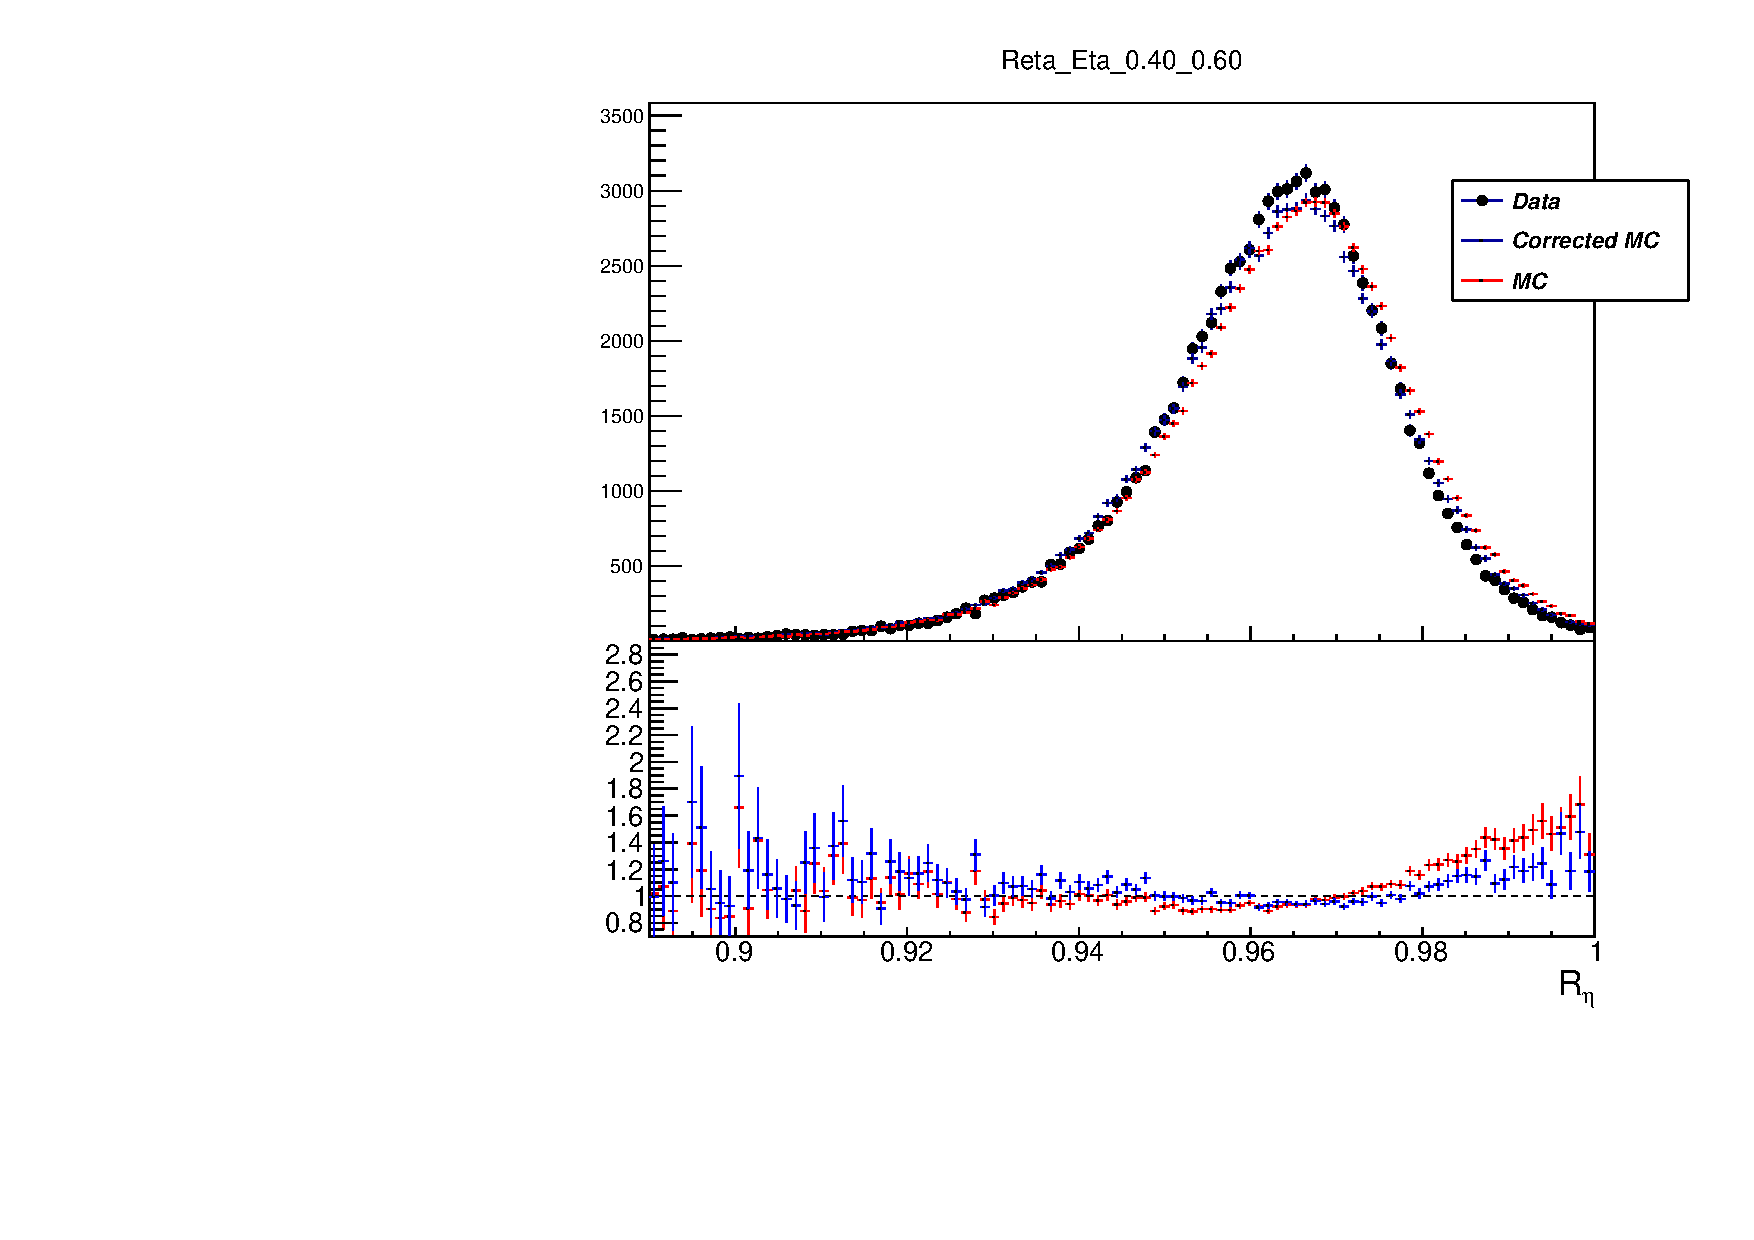
\includegraphics[width=\textwidth,keepaspectratio]{Reta_Eta_4_6_Athena.pdf}
  		\caption{Reweighted  $R_{\eta }$ in $|\eta| = (0.4,0.6)$.  }
  		\label{fig::id}
  	\end{subfigure}
  	\hfill
  	\begin{subfigure}[t]{0.5\textwidth} 
  		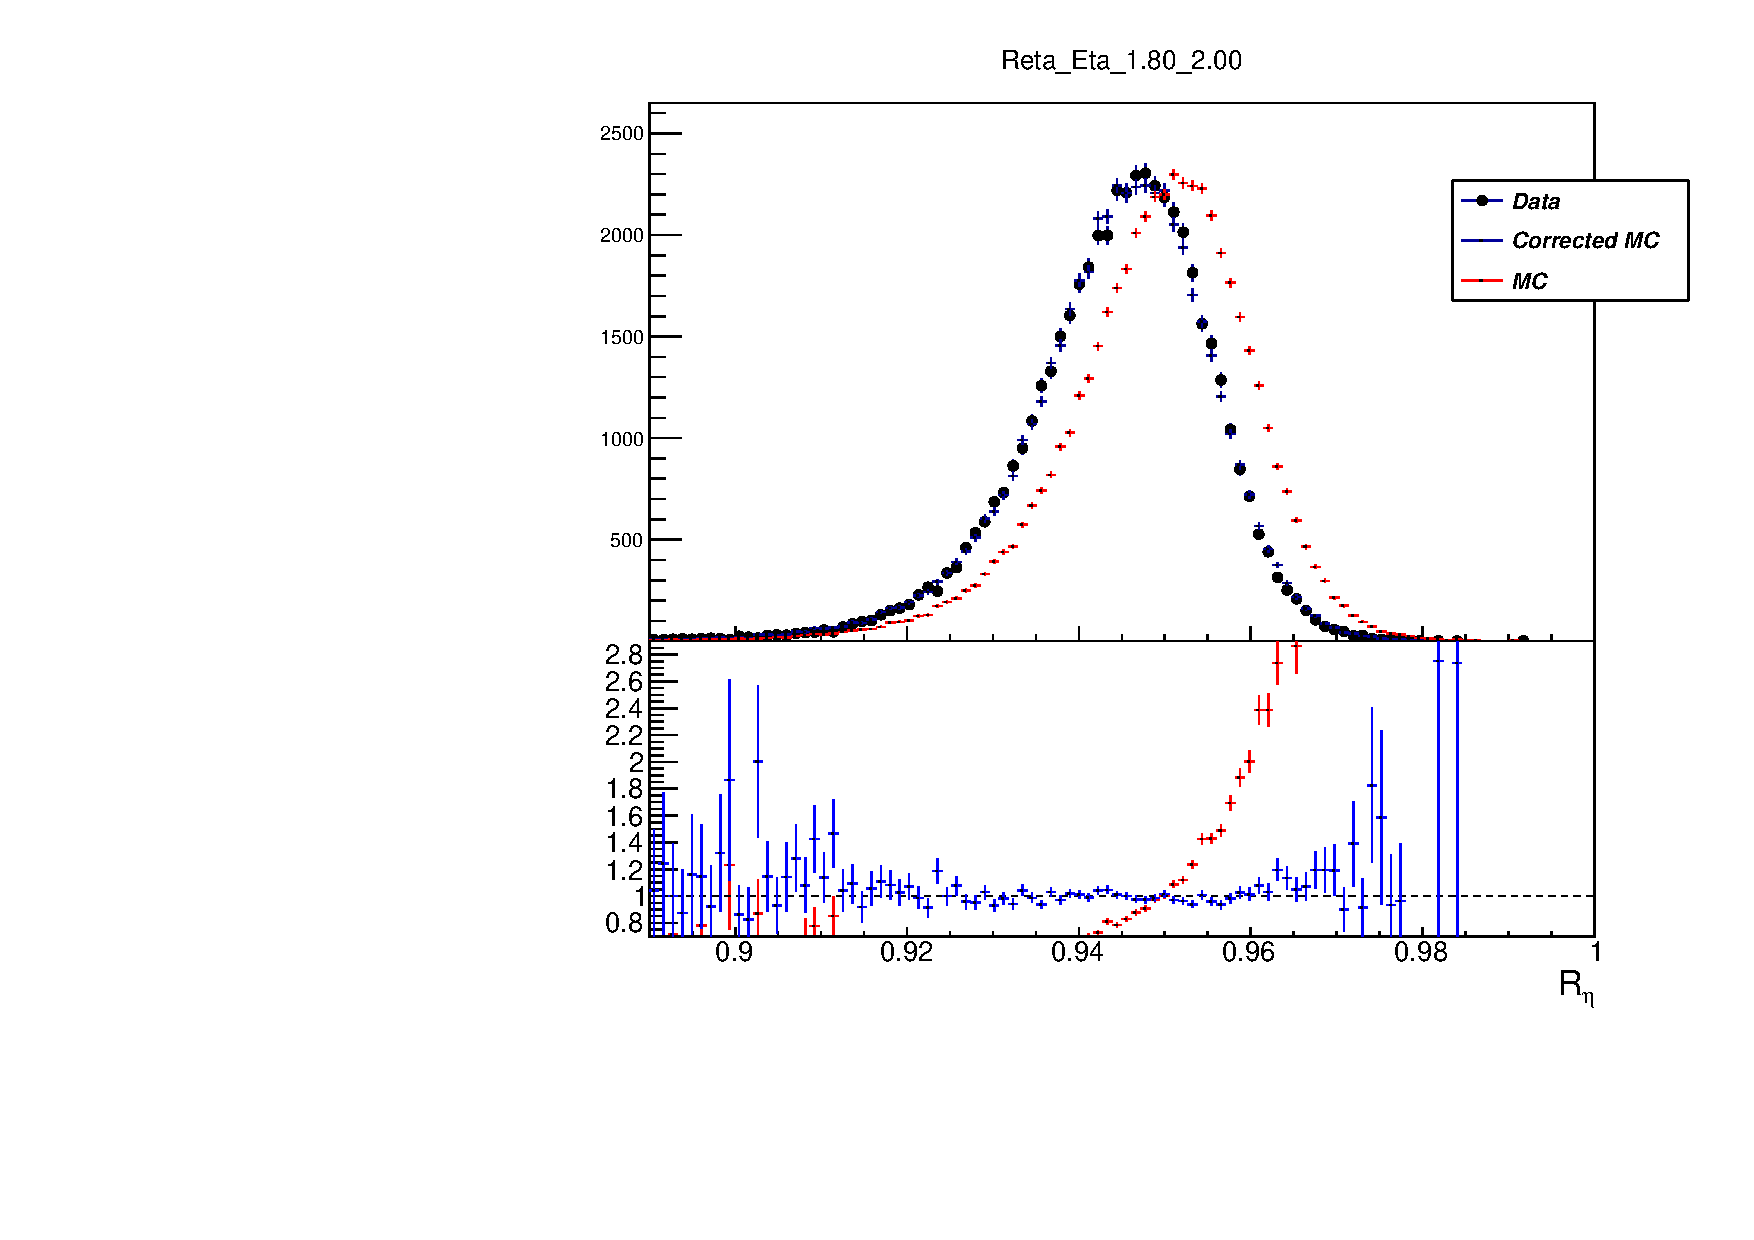
\includegraphics[width=\textwidth,keepaspectratio]{Reta_Eta_18_20_Athena.pdf}
  		\caption{Reweighted  $R_{\eta }$ in $|\eta| = (1.8,2.0)$.  }
  		\label{fig::pd}
  	\end{subfigure}
  	\caption{$R_{\eta }$  in the barrel and in the end-cap}
  	\label{fig::reta}
  \end{figure}
 
      \begin{figure}[htbp]
  	\begin{subfigure}[t]{0.5\textwidth}
  		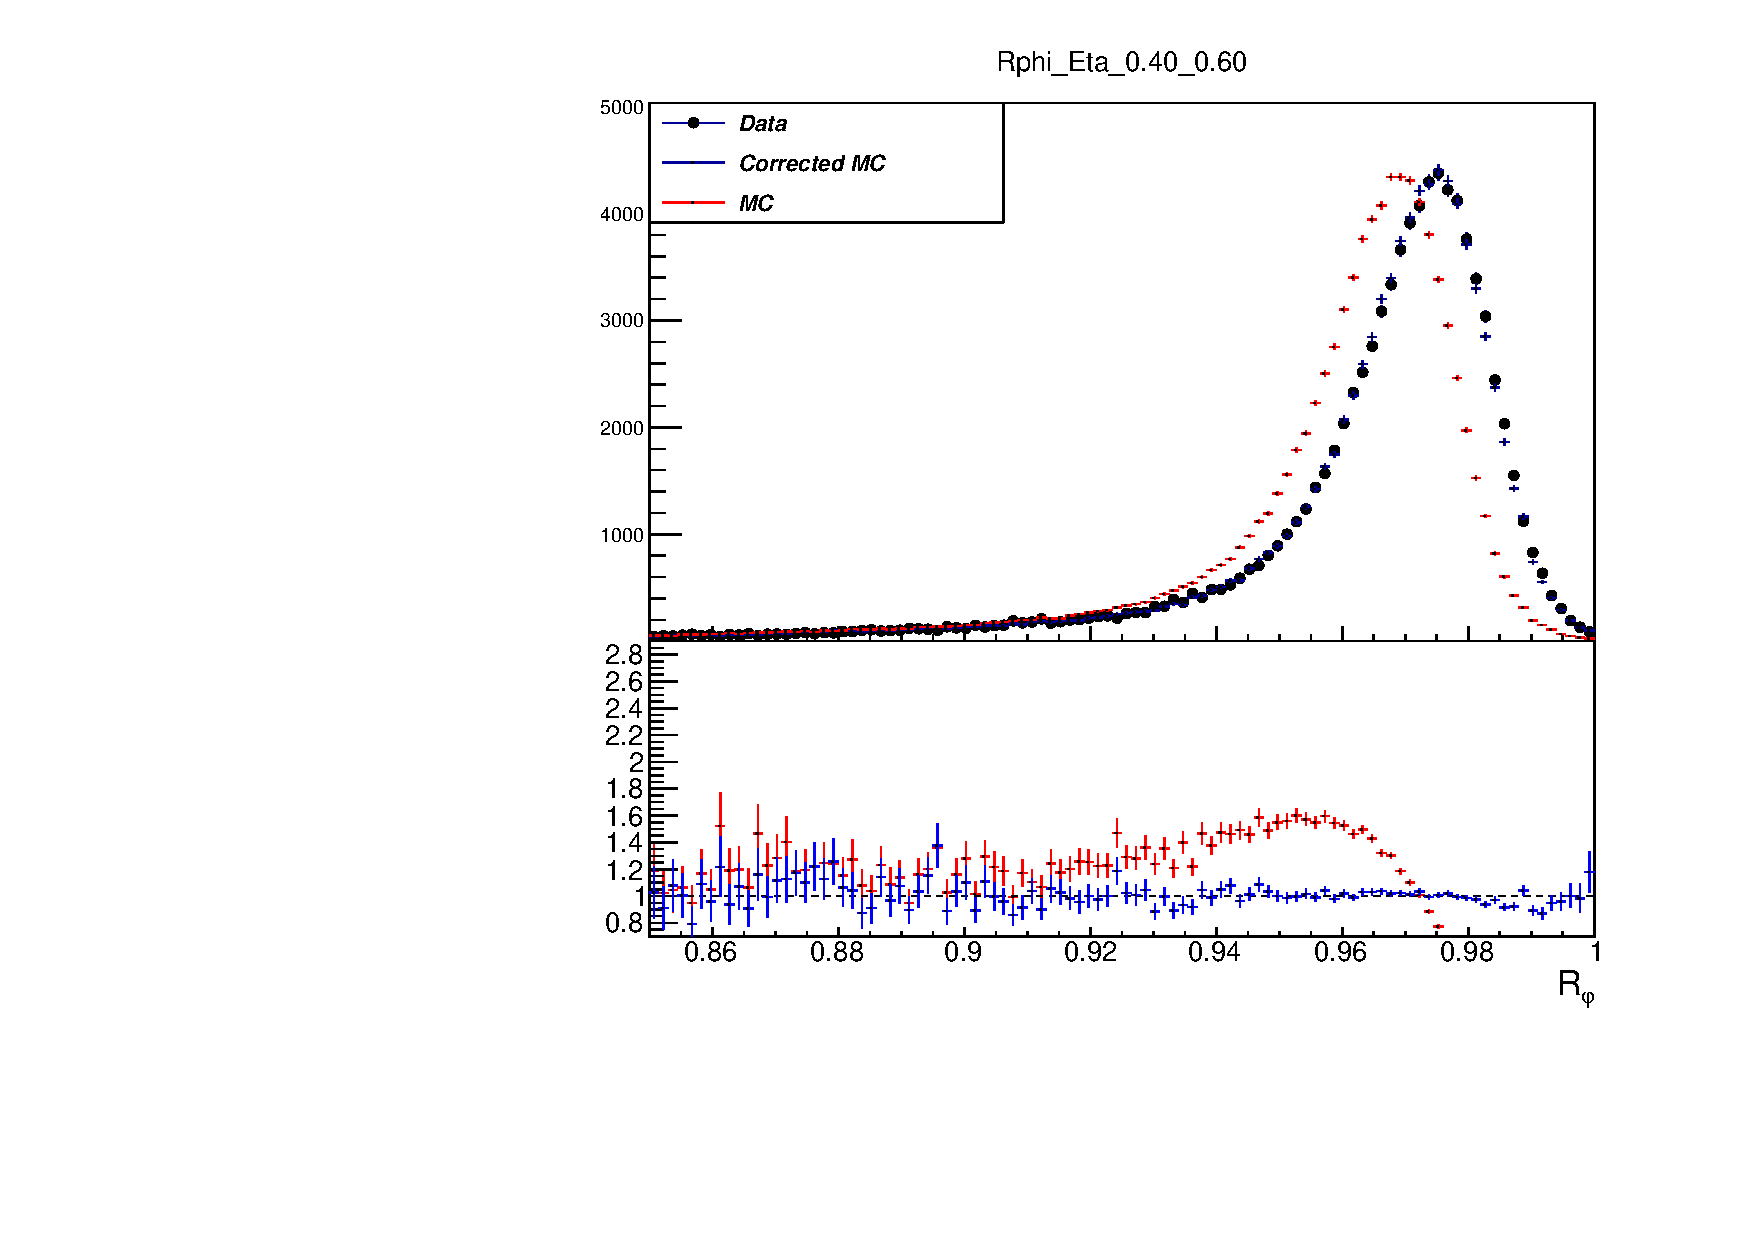
\includegraphics[width=\textwidth,keepaspectratio]{Rphi_Eta_4_6_Athena.pdf}
  		\caption{$R_{\phi}$ in $|\eta| = (0.4,0.6)$ }
  		\label{fig::rphi_rew_04}
  	\end{subfigure}
  	\hfill
  	\begin{subfigure}[t]{0.5\textwidth} 
  		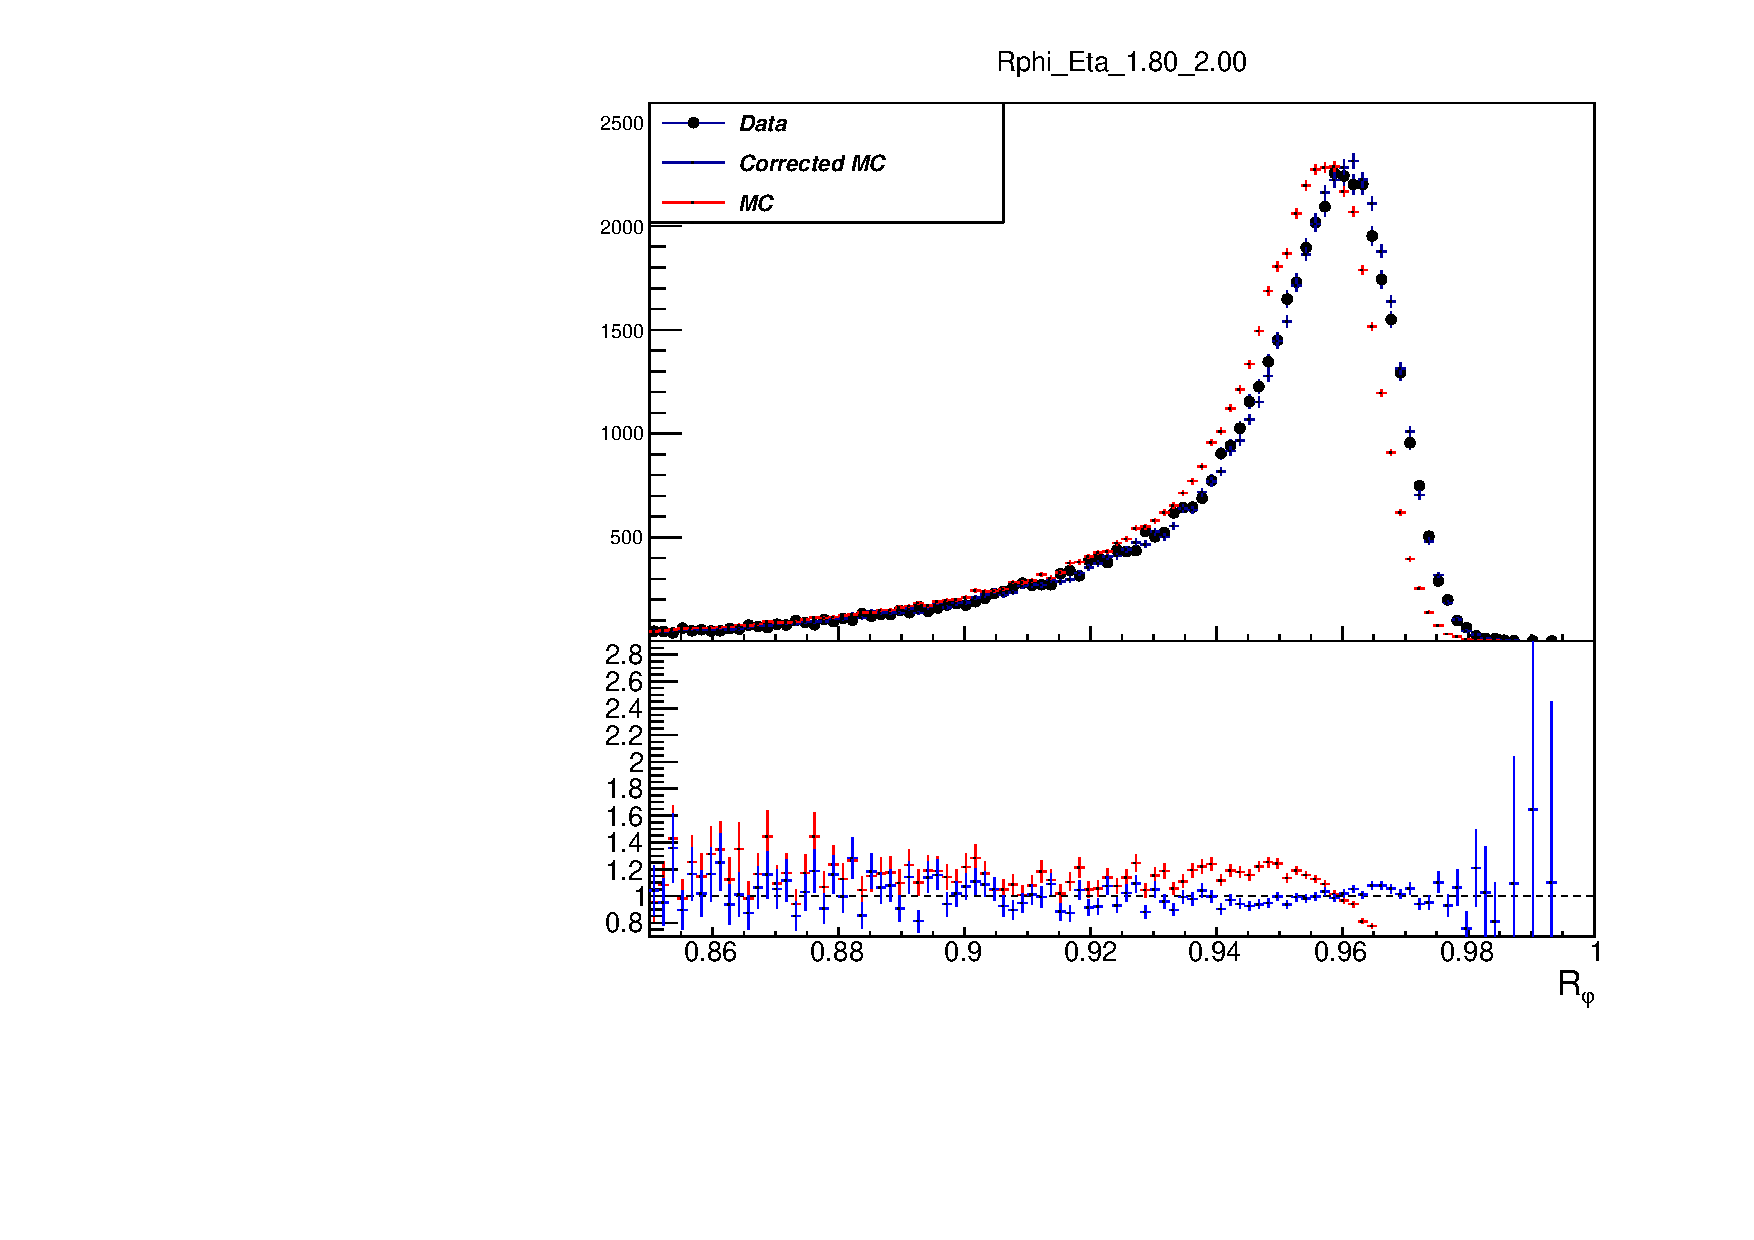
\includegraphics[width=\textwidth,keepaspectratio]{Rphi_Eta_18_20_Athena.pdf}
  		\caption{$R_{\phi}$ in $|\eta| = (1.8,2.0)$ }
  		\label{fig::rphi_rew_18}
  	\end{subfigure}
  	\caption{$R_{\phi}$ in the barel and in the end-cap, Data, MC, reweighted MC}
  	\label{fig::rphi_rew}
  \end{figure}
  
    \begin{figure}[htbp]
	\begin{subfigure}[t]{0.5\textwidth}
		\includegraphics[width=\textwidth,keepaspectratio]{weta2_Eta_4_6_Athena.pdf}
		\caption{$W_{\eta}^2$ in $|\eta| = (0.4,0.6)$ }
		\label{fig::weta2_rew_04}
	\end{subfigure}
	\hfill
	\begin{subfigure}[t]{0.5\textwidth} 
		\includegraphics[width=\textwidth,keepaspectratio]{weta2_Eta_18_20.pdf}
		\caption{$W_{\eta}^2$ in $|\eta| = (1.8,2.0)$ }
		\label{fig::weta2_rew_18}
	\end{subfigure}
	\caption{$W_{\eta}^2$ in the barel and in the end-cap, Data, MC, reweighted MC}
	\label{fig::weta2_rew}
\end{figure}

\begin{figure*}[ht!]
	\subfloat{%
		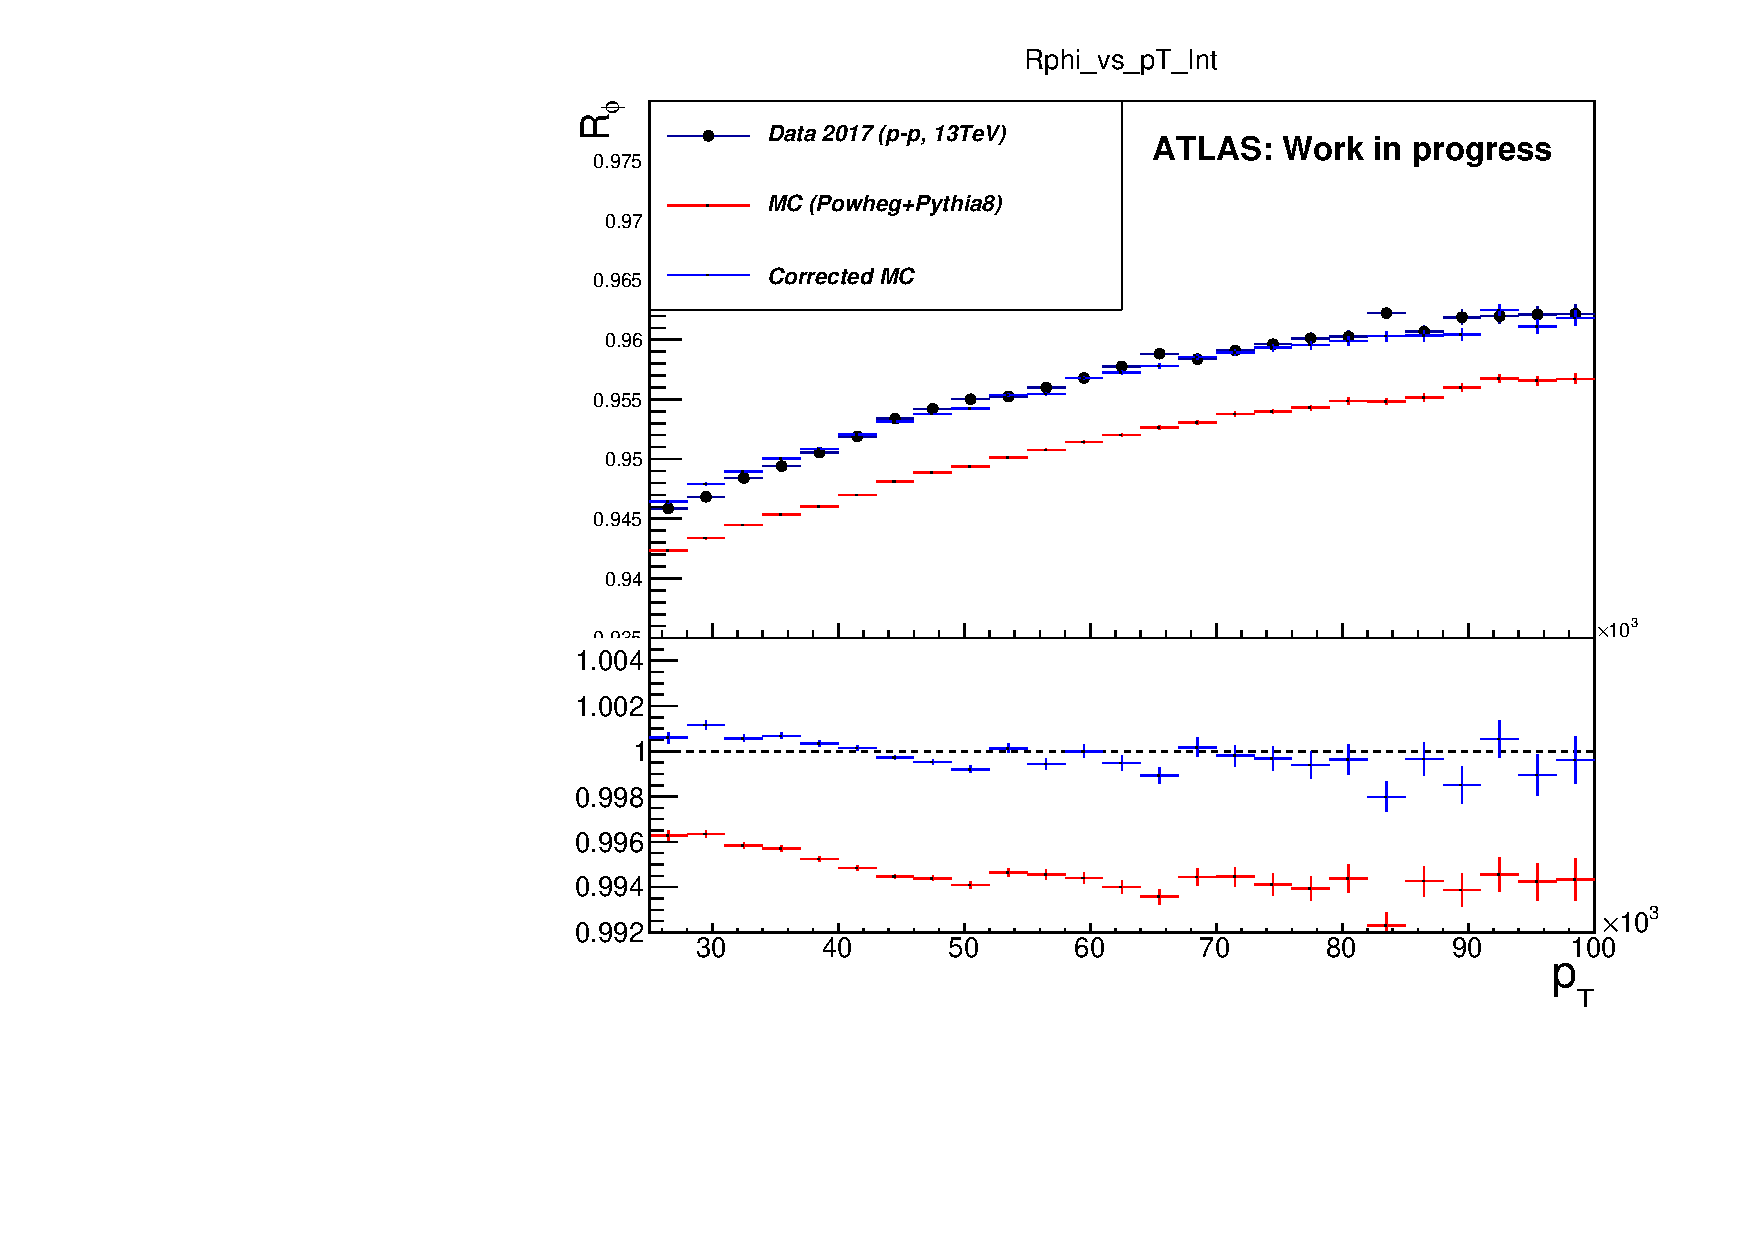
\includegraphics[width=0.33\textwidth]{Rphi_vs_pT_Int}}
	\quad
	\subfloat {%
		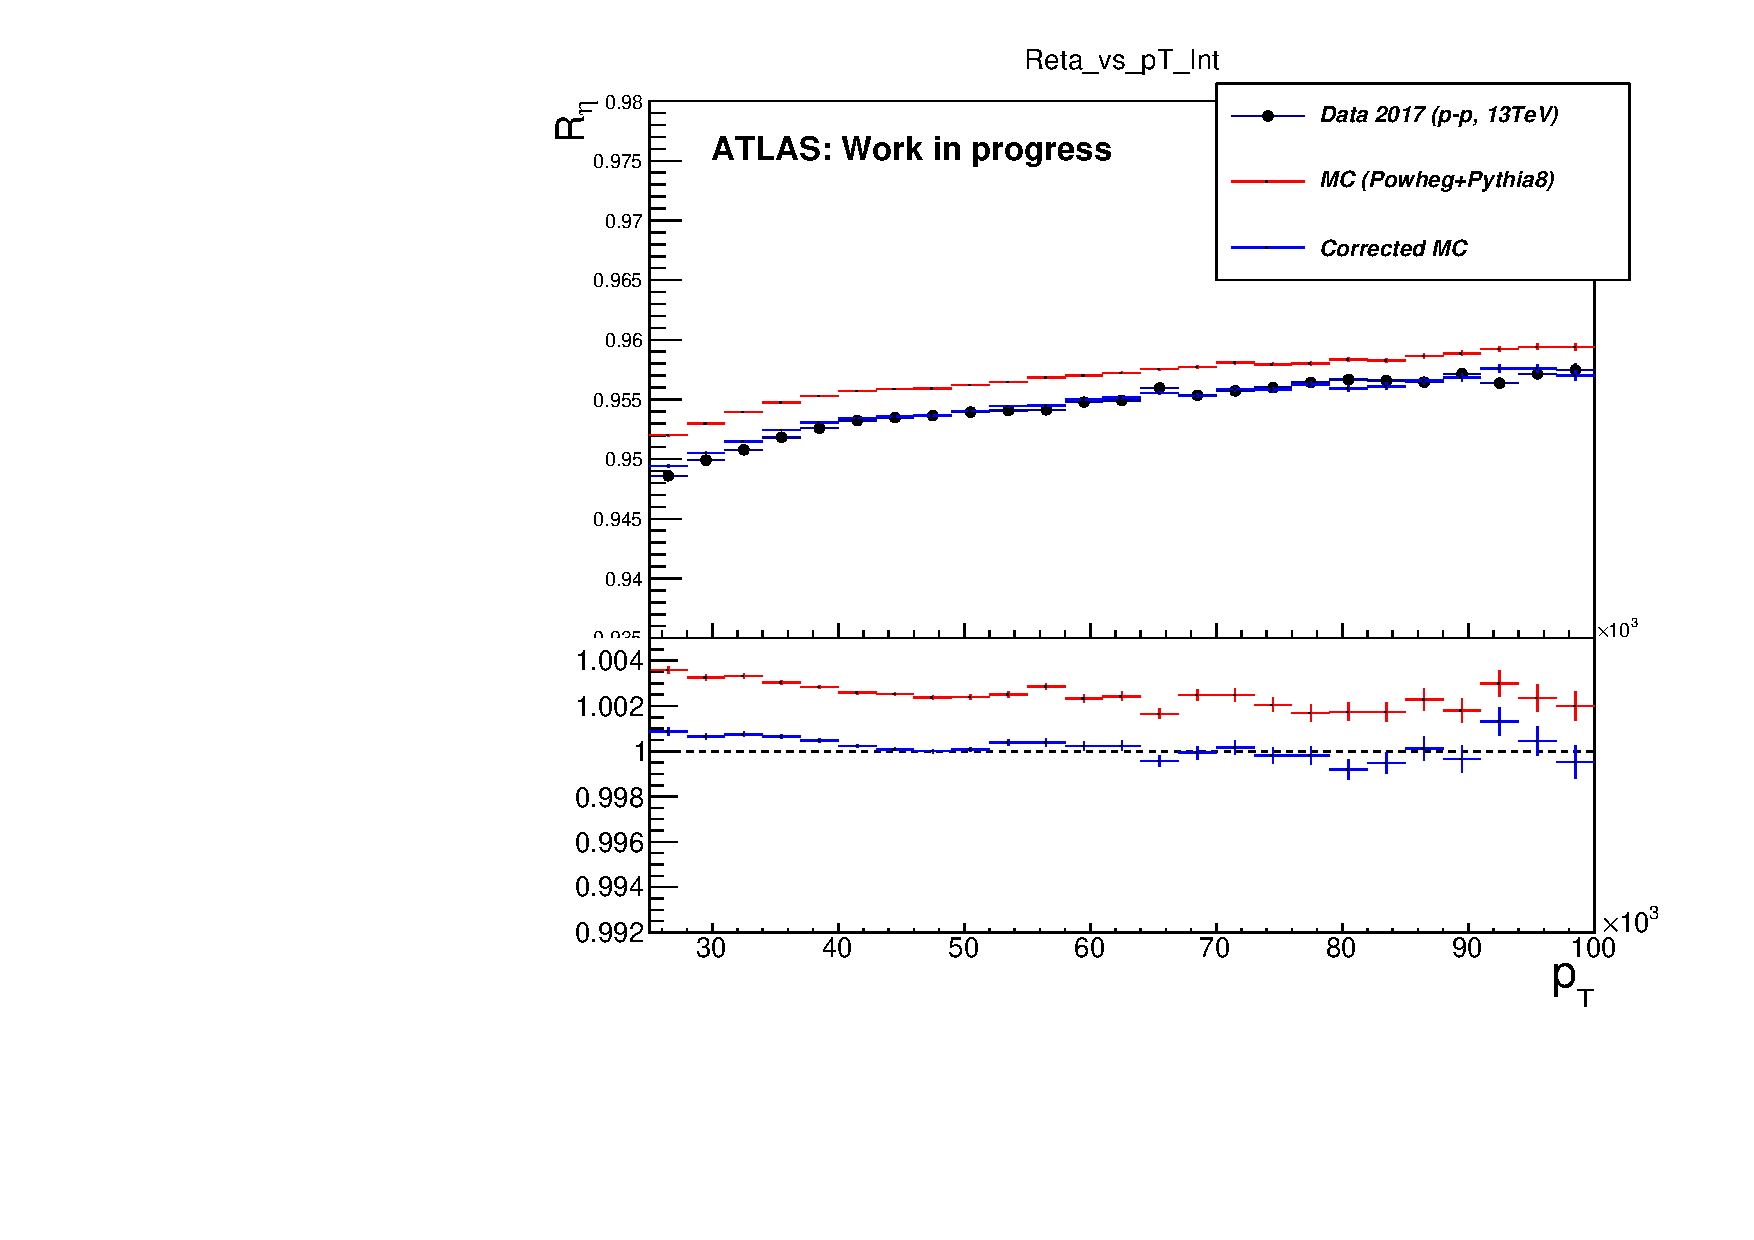
\includegraphics[width=0.33\textwidth]{Reta_vs_pT_Int}}
	\quad
	\subfloat{%
		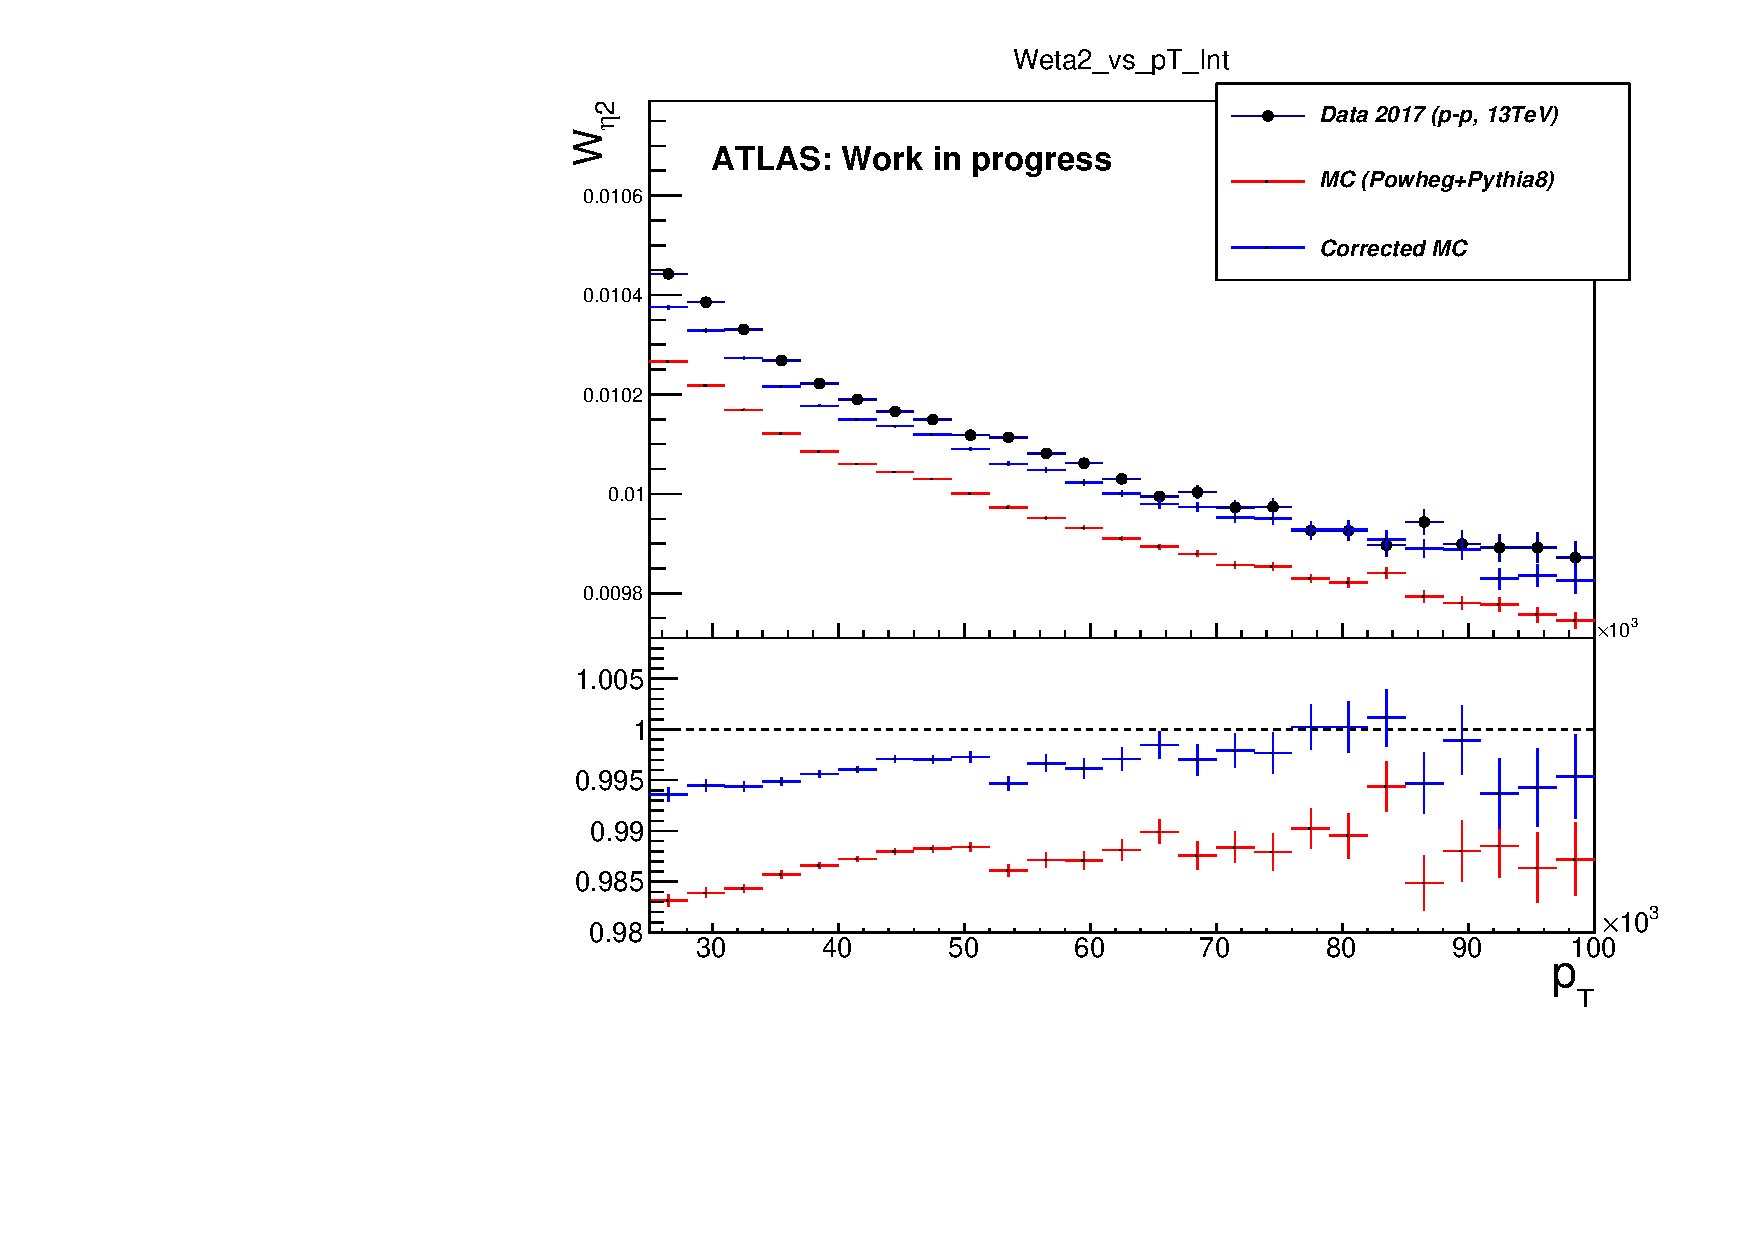
\includegraphics[width=0.33\textwidth]{Weta2_vs_pT_Int}}\\

	\caption{ 	\label{fig::integrated} Distributions integrated over pT (a) $R_{\phi}$; (b) $R_{\eta}$; (c)$W_{\eta 2}$.}
\end{figure*}


  
  \begin{figure}[htbp]
  	\centering
  	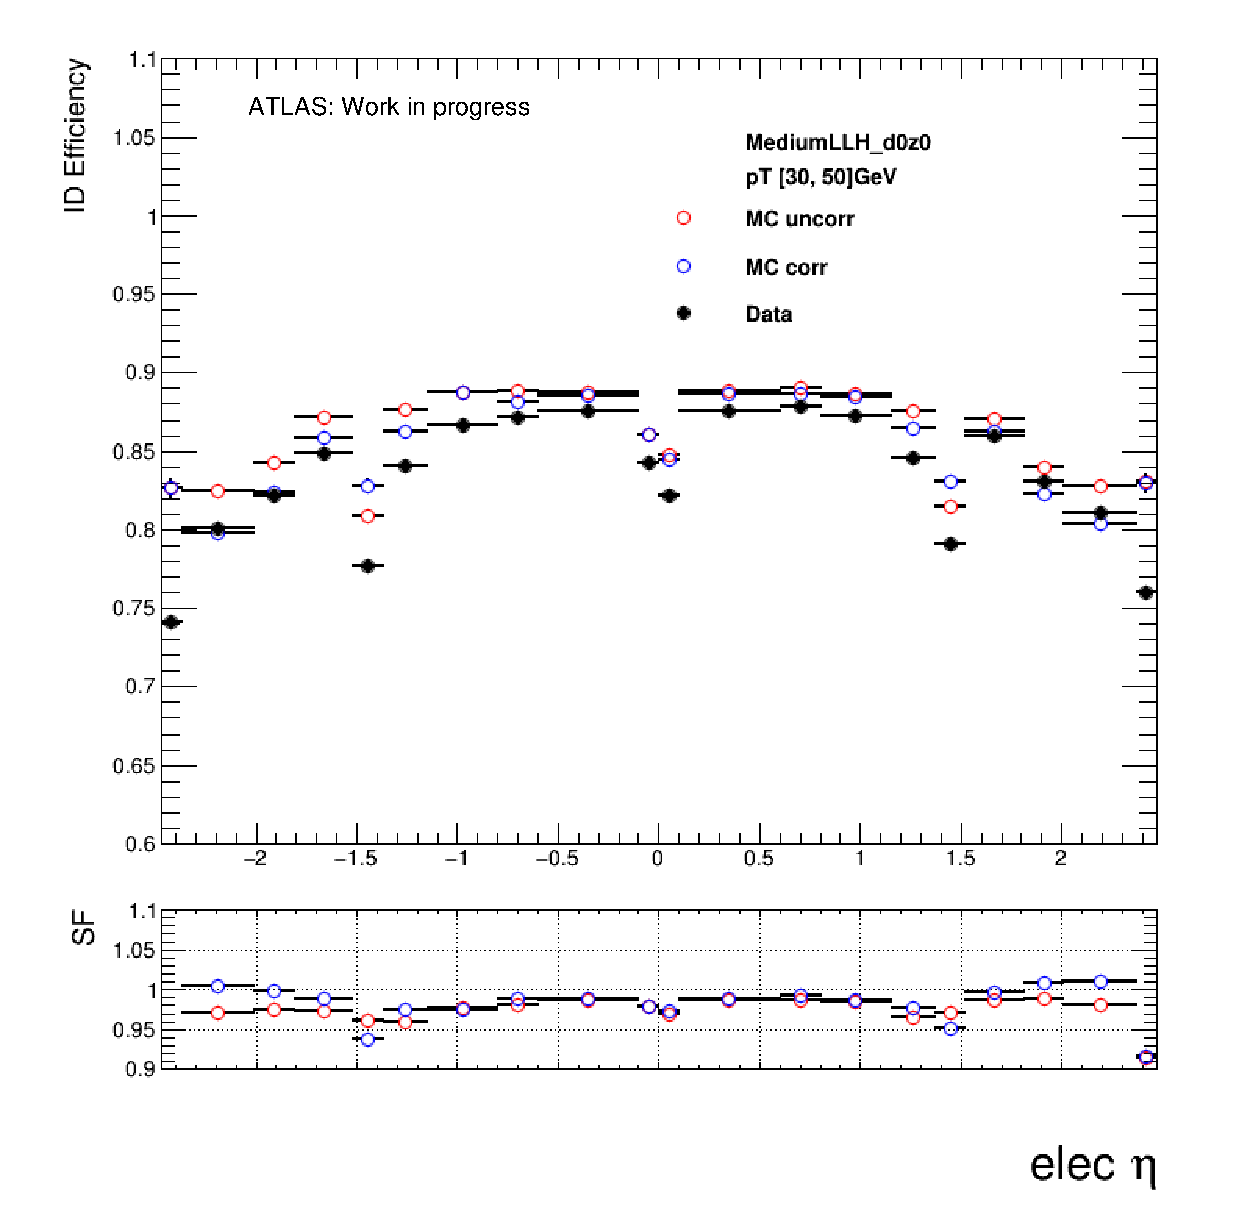
\includegraphics[width=7cm,keepaspectratio]{MCeffm247tom237.pdf}\\
  	\caption{Electron identification efficiency as a function of the electron pseudo-rapidity}
  	\label{SF}
  \end{figure}
  \section{Appendix: control plots}

  \begin{figure*}[ht!]
  	\subfloat{%
  		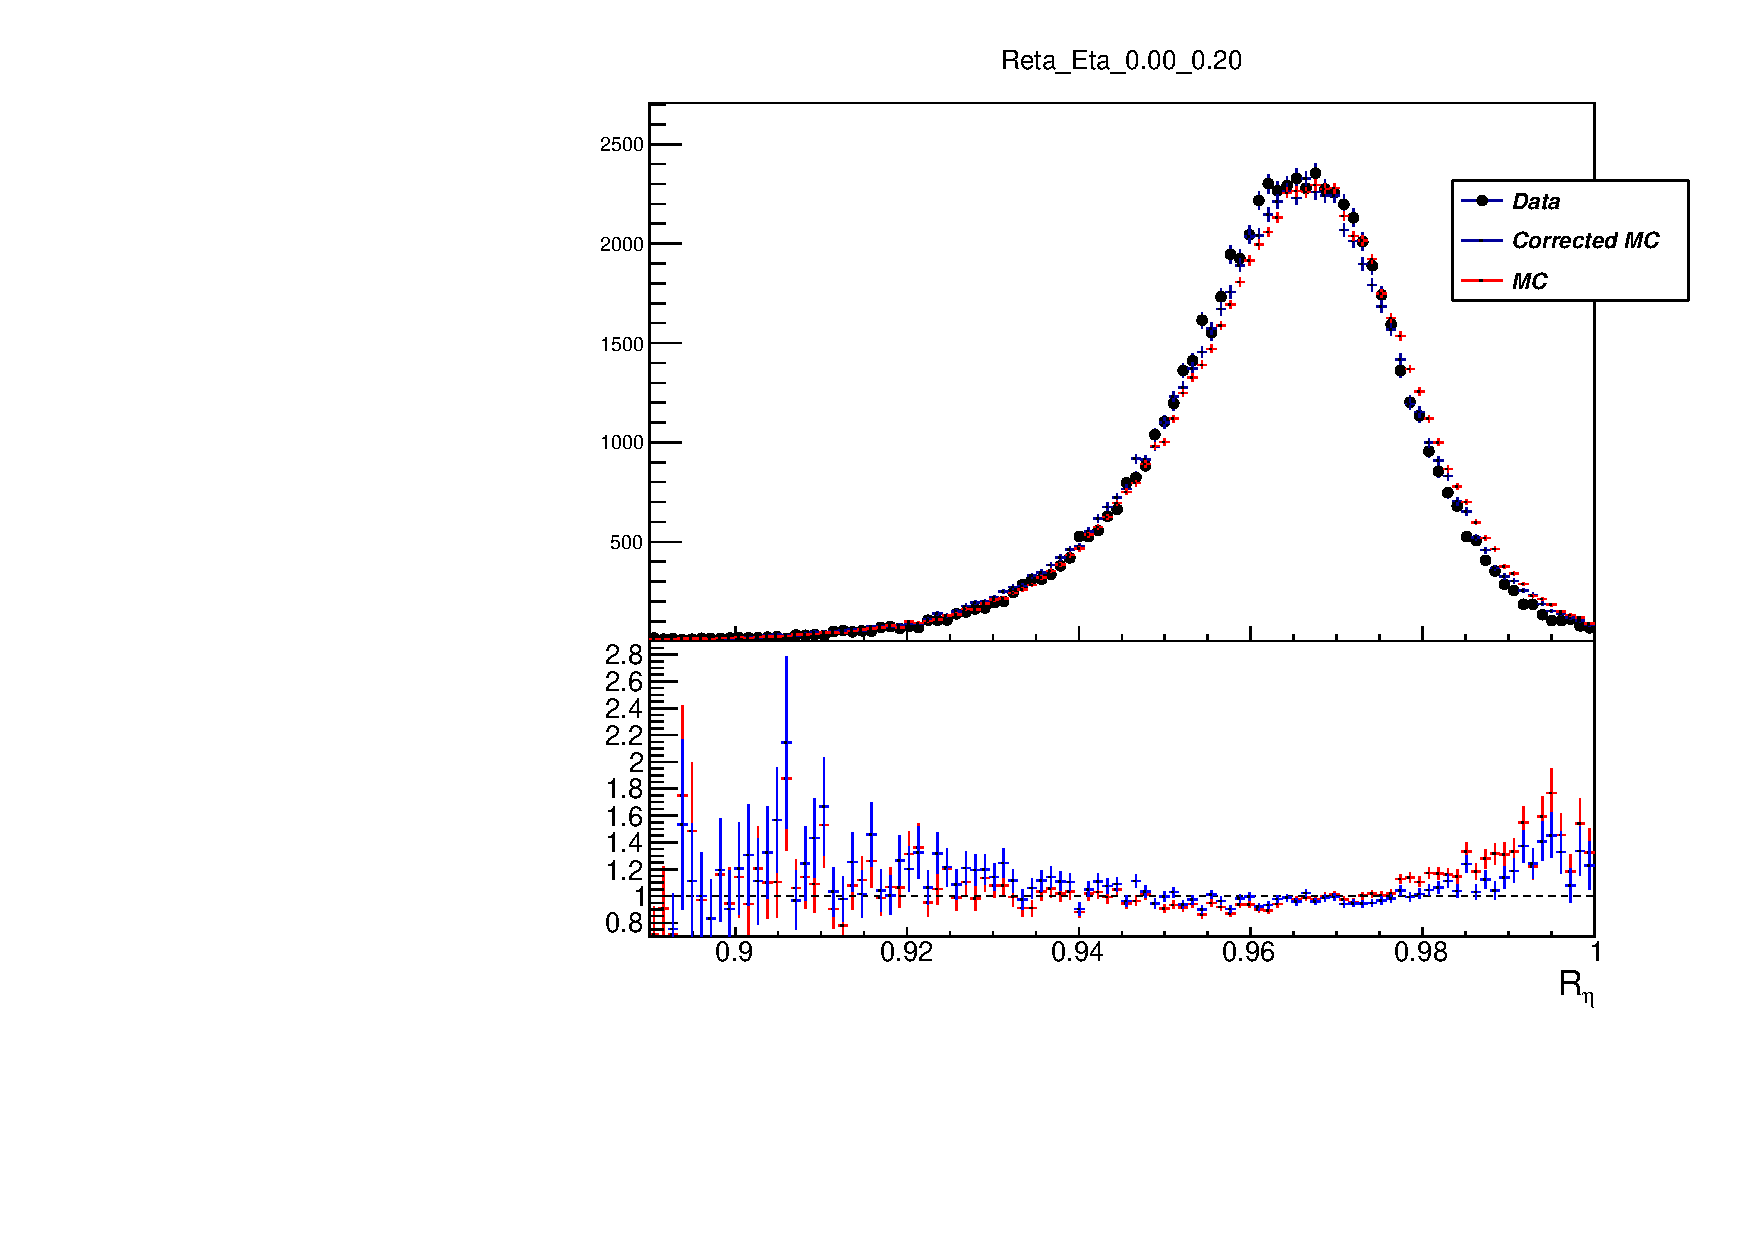
\includegraphics[width=0.33\textwidth]{Reta_Eta_0_2_Athena}}
  	\quad
  	\subfloat {%
  		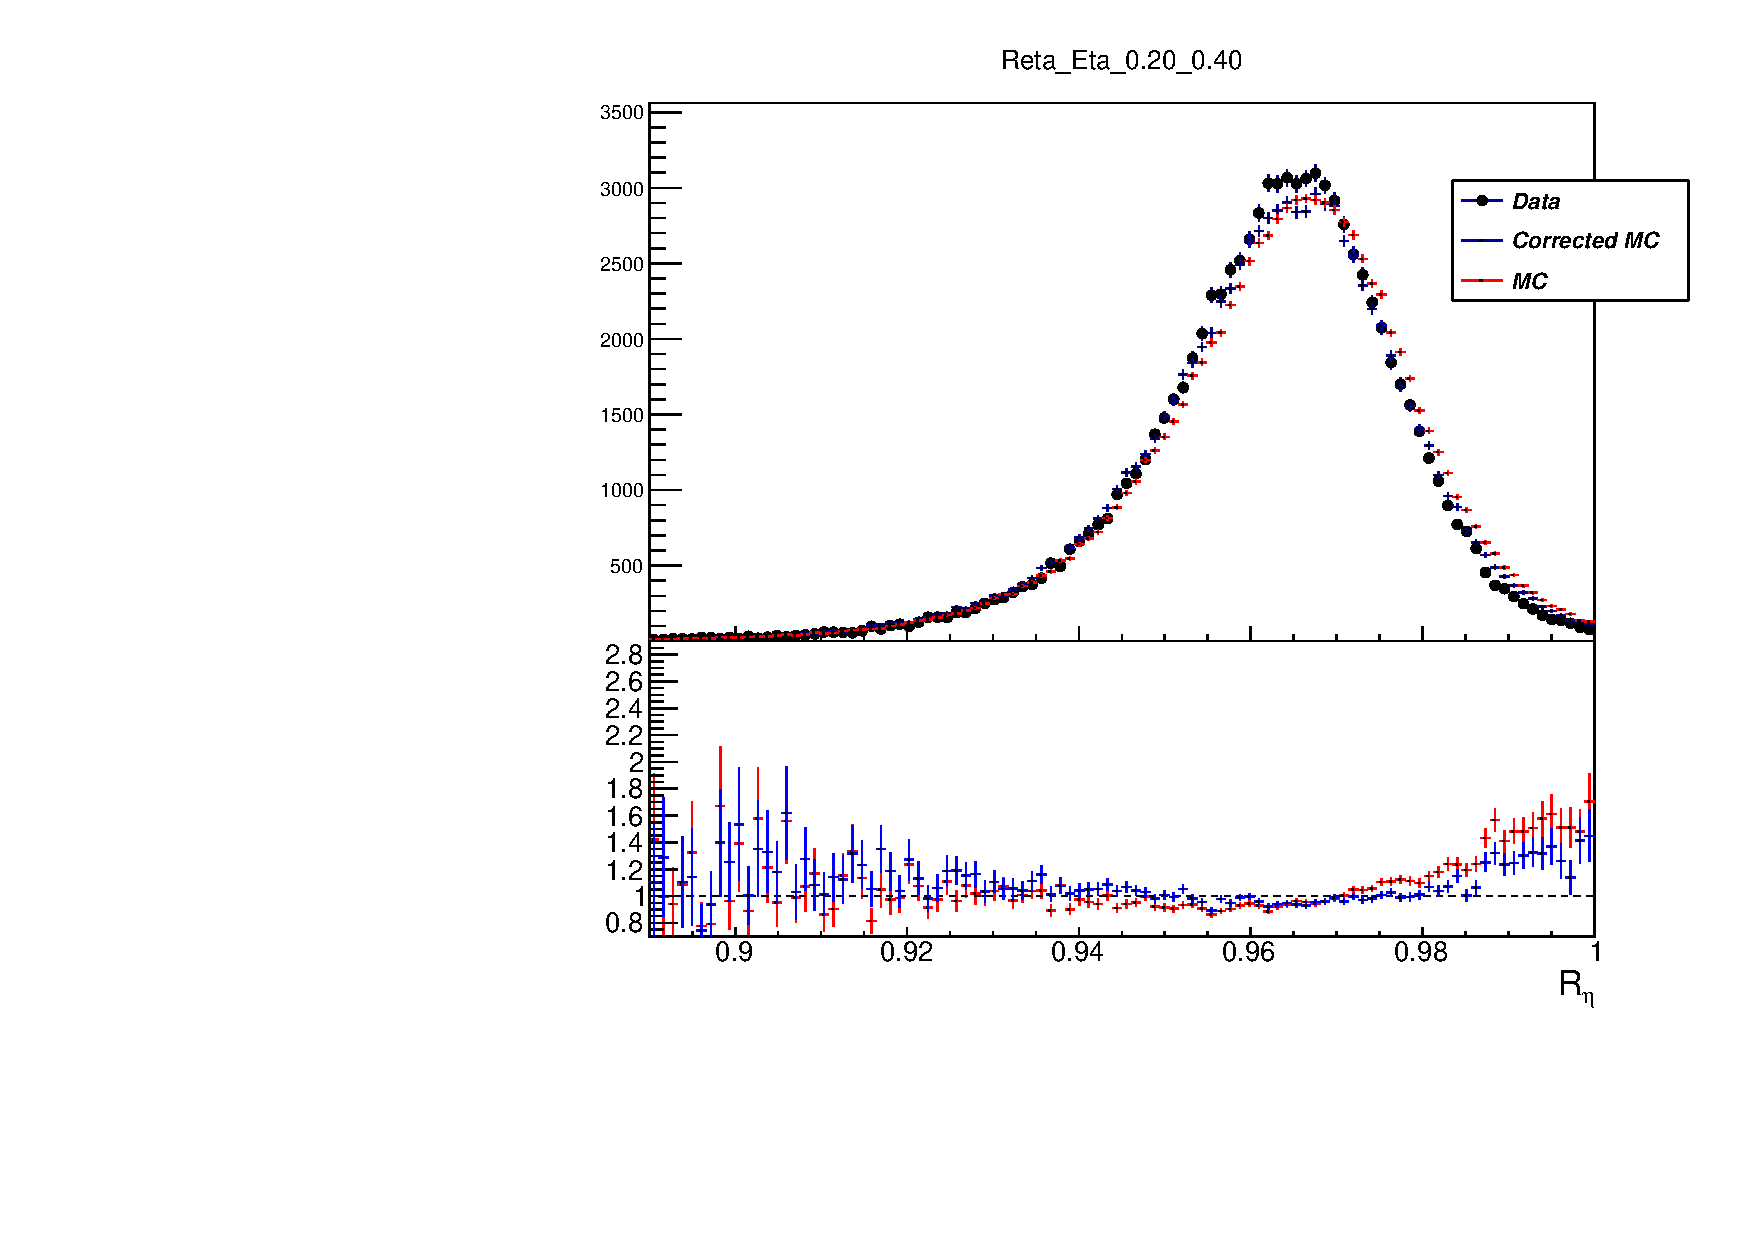
\includegraphics[width=0.33\textwidth]{Reta_Eta_2_4_Athena}}
  	\quad
  	\subfloat{%
  		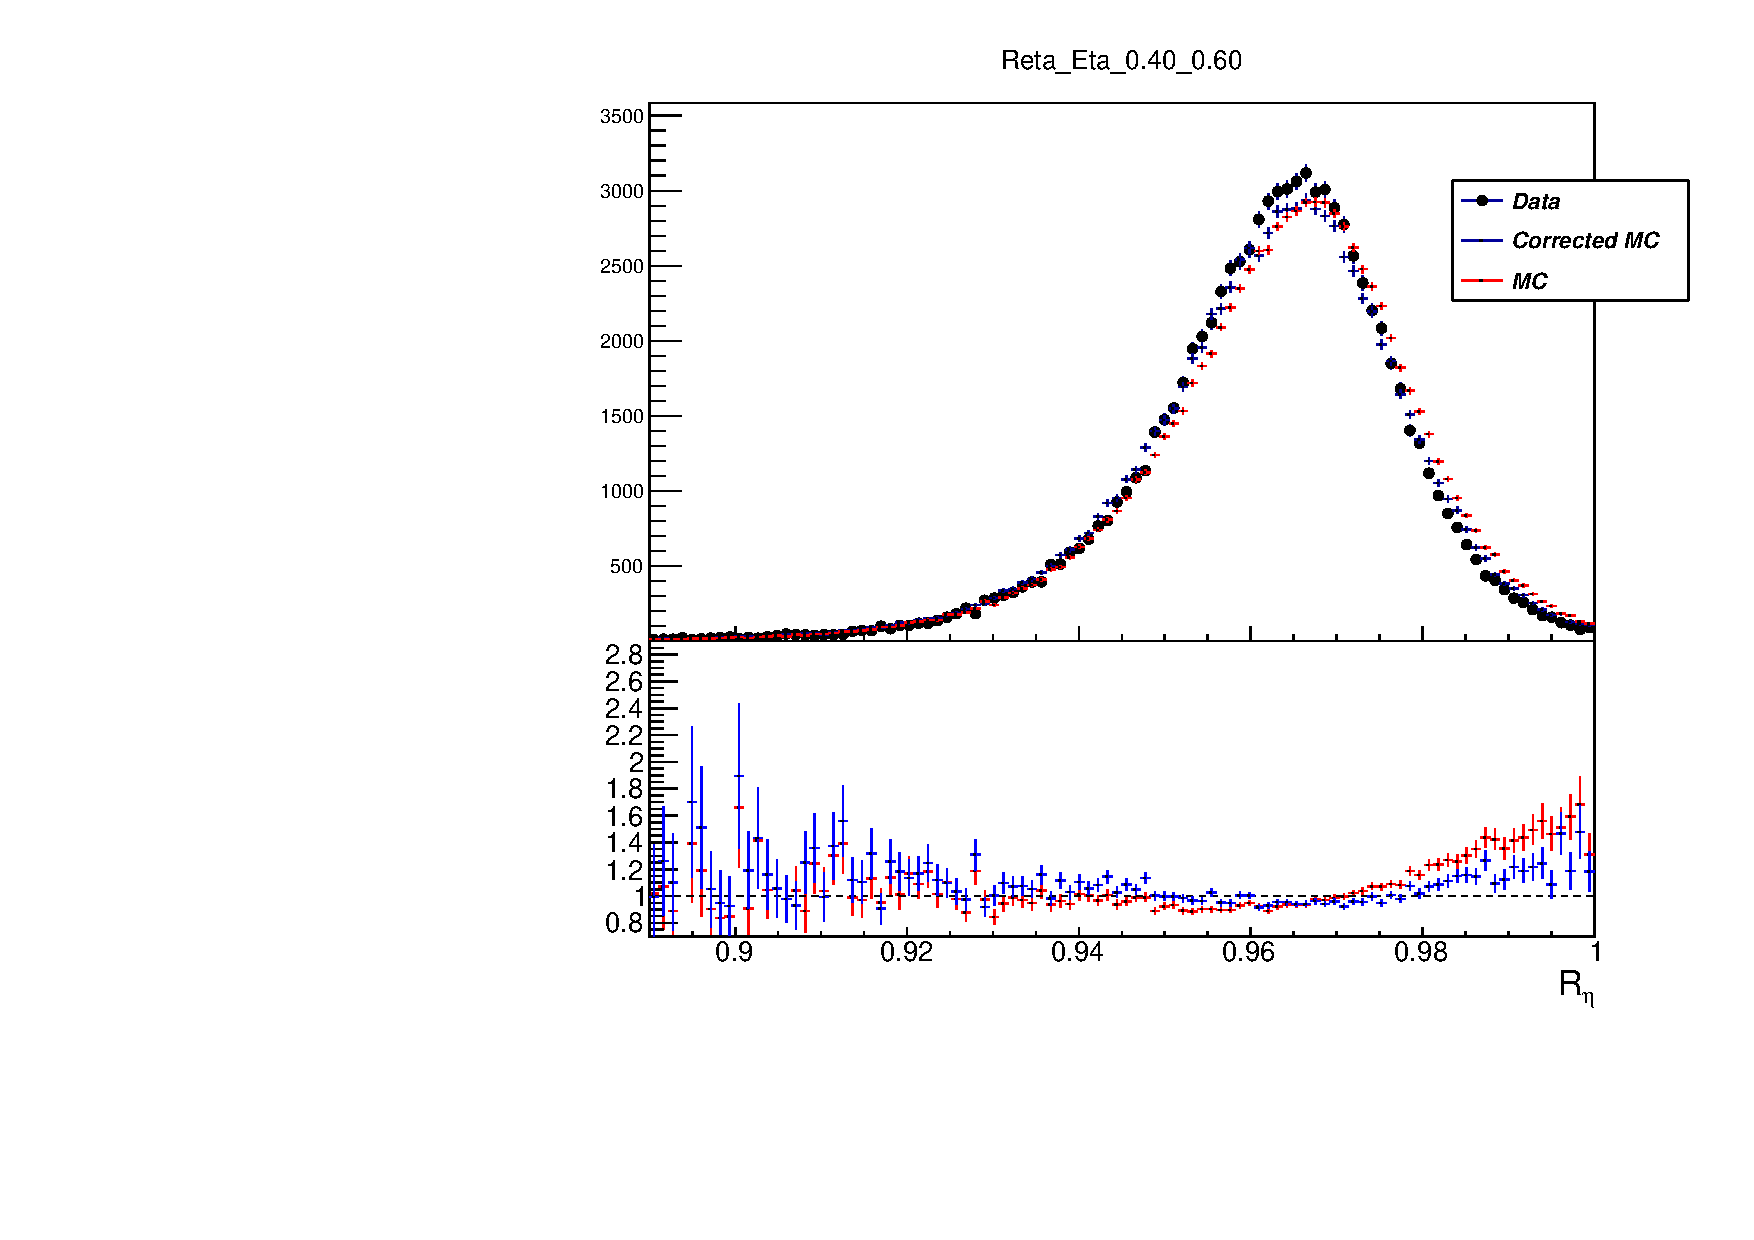
\includegraphics[width=0.33\textwidth]{Reta_Eta_4_6_Athena}}\\
  	\subfloat{%
  		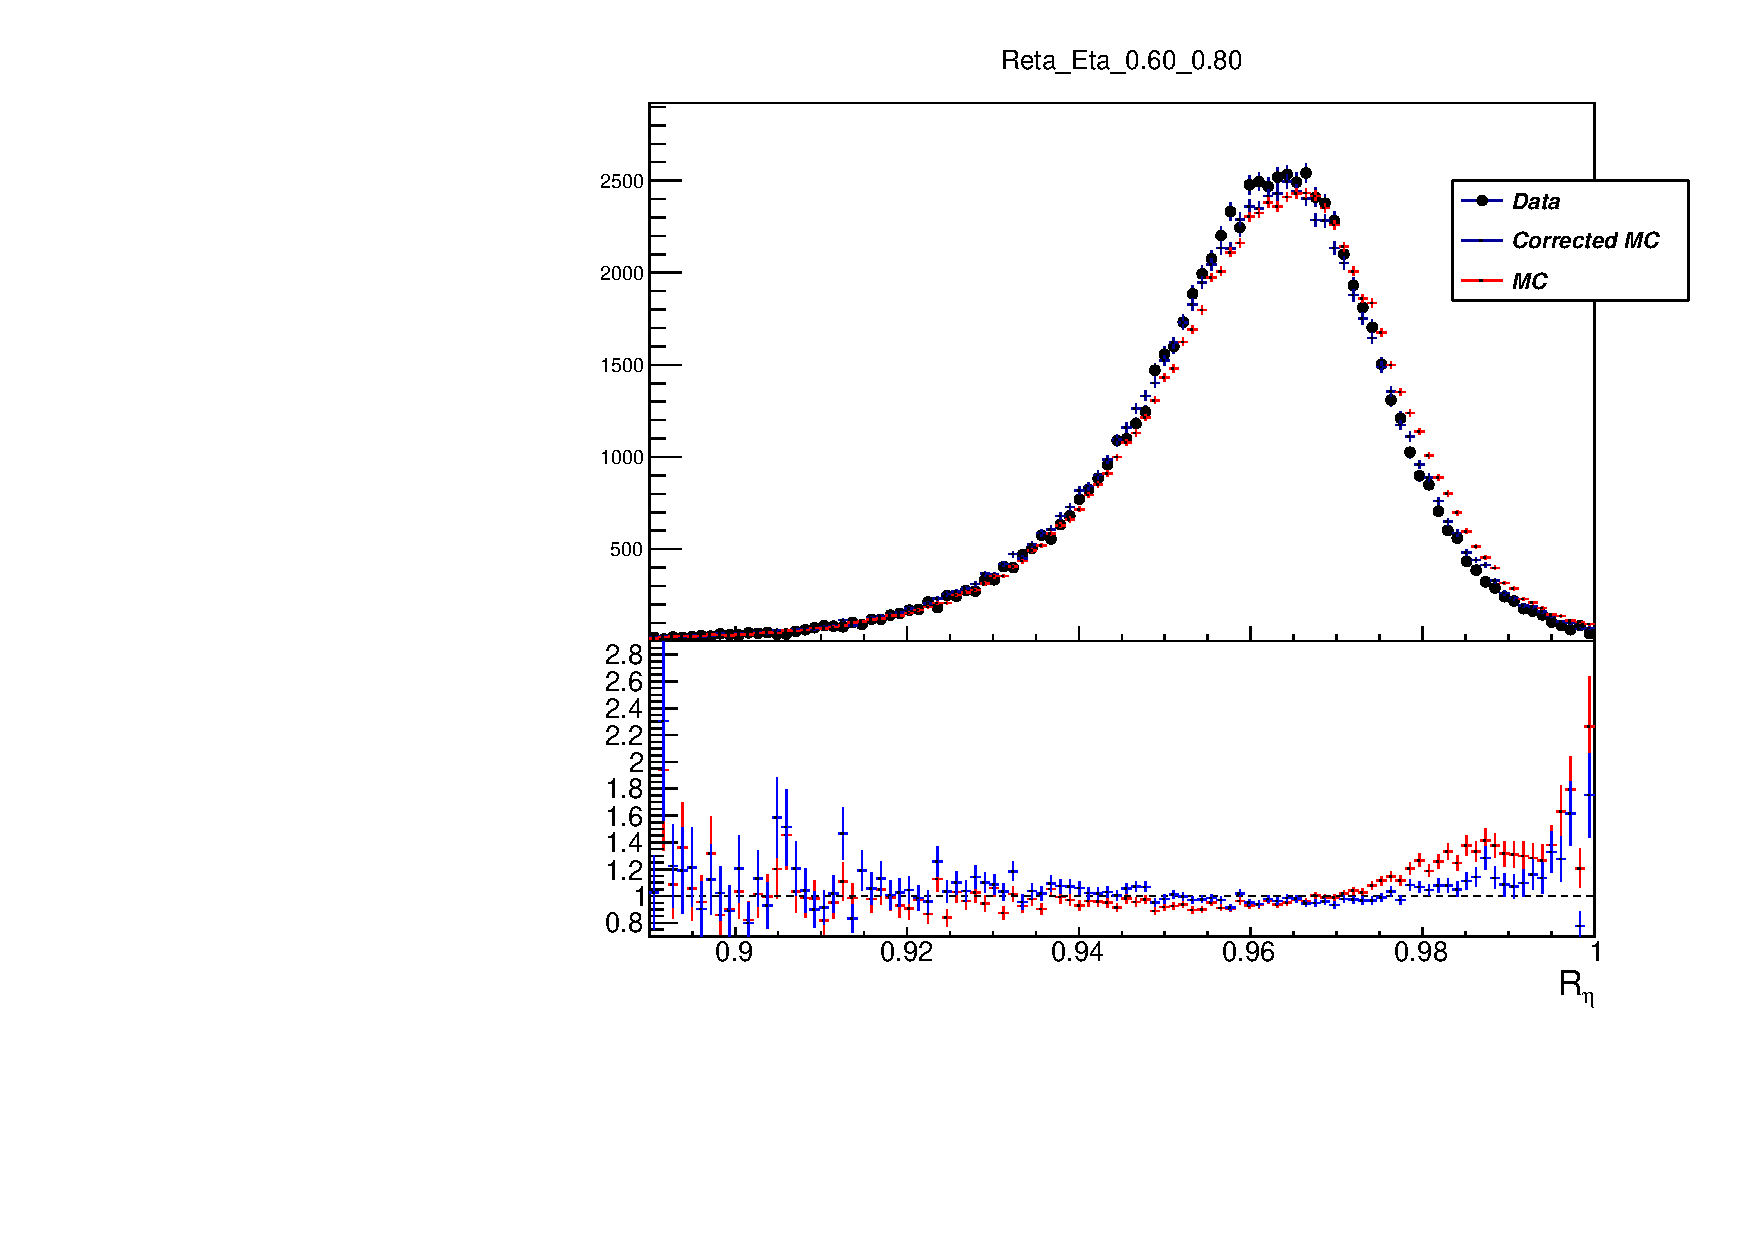
\includegraphics[width=0.33\textwidth]{Reta_Eta_6_8_Athena}}
  	\quad
  	\subfloat {%
  		\includegraphics[width=0.33\textwidth]{Reta_Eta_8_10_Athena}}
  	\quad
  	\subfloat{%
  		\includegraphics[width=0.33\textwidth]{Reta_Eta_10_12_Athena}}\\
	\subfloat{%
		\includegraphics[width=0.33\textwidth]{Reta_Eta_12_13_Athena}}
	\quad
	\subfloat{%
		\includegraphics[width=0.33\textwidth]{Reta_Eta_152_16_Athena}}
	\subfloat{%
			\includegraphics[width=0.33\textwidth]{Reta_Eta_16_18_Athena}}\\
	\quad
	\subfloat {%
		\includegraphics[width=0.33\textwidth]{Reta_Eta_16_18_Athena}}
	\quad
	\subfloat{%
		\includegraphics[width=0.33\textwidth]{Reta_Eta_20_22_Athena}}
		\quad
	\subfloat{%
		\includegraphics[width=0.33\textwidth]{Reta_Eta_22_24_Athena}}
	\caption{ 	\label{fig::reta_} Reta 2}
\end{figure*}

  \begin{figure*}[ht!]
	\subfloat{%
		\includegraphics[width=0.33\textwidth]{Rphi_Eta_0_2_Athena}}
	\quad
	\subfloat {%
		\includegraphics[width=0.33\textwidth]{Rphi_Eta_2_4_Athena}}
	\quad
	\subfloat{%
		\includegraphics[width=0.33\textwidth]{Rphi_Eta_4_6_Athena}}\\
	\subfloat{%
		\includegraphics[width=0.33\textwidth]{Rphi_Eta_6_8_Athena}}
	\quad
	\subfloat {%
		\includegraphics[width=0.33\textwidth]{Rphi_Eta_8_10_Athena}}
	\quad
	\subfloat{%
		\includegraphics[width=0.33\textwidth]{Rphi_Eta_10_12_Athena}}\\
	\subfloat{%
		\includegraphics[width=0.33\textwidth]{Rphi_Eta_12_13_Athena}}
	\quad
	\subfloat{%
		\includegraphics[width=0.33\textwidth]{Rphi_Eta_152_16_Athena}}
	\subfloat{%
		\includegraphics[width=0.33\textwidth]{Rphi_Eta_16_18_Athena}}\\
	\quad
	\subfloat {%
		\includegraphics[width=0.33\textwidth]{Rphi_Eta_16_18_Athena}}
	\quad
	\subfloat{%
		\includegraphics[width=0.33\textwidth]{Rphi_Eta_20_22_Athena}}
	\quad
	\subfloat{%
		\includegraphics[width=0.33\textwidth]{Rphi_Eta_22_24_Athena}}
	\caption{ 	\label{fig::rphi_} Rphi in all eta slices}
\end{figure*}

  \begin{figure*}[ht!]
	\subfloat{%
		\includegraphics[width=0.33\textwidth]{Weta2_Eta_0_2_Athena}}
	\quad
	\subfloat {%
		\includegraphics[width=0.33\textwidth]{Weta2_Eta_2_4_Athena}}
	\quad
	\subfloat{%
		\includegraphics[width=0.33\textwidth]{Weta2_Eta_4_6_Athena}}\\
	\subfloat{%
		\includegraphics[width=0.33\textwidth]{Weta2_Eta_6_8_Athena}}
	\quad
	\subfloat {%
		\includegraphics[width=0.33\textwidth]{Weta2_Eta_8_10_Athena}}
	\quad
	\subfloat{%
		\includegraphics[width=0.33\textwidth]{Weta2_Eta_10_12_Athena}}\\
	\subfloat{%
		\includegraphics[width=0.33\textwidth]{Weta2_Eta_12_13_Athena}}
	\quad
	\subfloat{%
		\includegraphics[width=0.33\textwidth]{Weta2_Eta_152_16_Athena}}
	\subfloat{%
		\includegraphics[width=0.33\textwidth]{Weta2_Eta_16_18_Athena}}\\
	\quad
	\subfloat {%
		\includegraphics[width=0.33\textwidth]{Weta2_Eta_16_18_Athena}}
	\quad
	\subfloat{%
		\includegraphics[width=0.33\textwidth]{Weta2_Eta_20_22_Athena}}
	\quad
	\subfloat{%
		\includegraphics[width=0.33\textwidth]{Weta2_Eta_22_24_Athena}}
	\caption{ 	\label{fig::weta2_} Reta 2}
\end{figure*}

  \begin{figure*}[ht!]
	\subfloat{%
		\includegraphics[width=0.33\textwidth]{Weta2_Eta_0_2_Athena}}
	\quad
	\subfloat {%
		\includegraphics[width=0.33\textwidth]{Weta2_Eta_2_4_Athena}}
	\quad
	\subfloat{%
		\includegraphics[width=0.33\textwidth]{Weta2_Eta_4_6_Athena}}\\
	\subfloat{%
		\includegraphics[width=0.33\textwidth]{Weta2_Eta_6_8_Athena}}
	\quad
	\subfloat {%
		\includegraphics[width=0.33\textwidth]{Weta2_Eta_8_10_Athena}}
	\quad
	\subfloat{%
		\includegraphics[width=0.33\textwidth]{Weta2_Eta_10_12_Athena}}\\
	\subfloat{%
		\includegraphics[width=0.33\textwidth]{Weta2_Eta_12_13_Athena}}
	\quad
	\subfloat{%
		\includegraphics[width=0.33\textwidth]{Weta2_Eta_152_16_Athena}}
	\subfloat{%
		\includegraphics[width=0.33\textwidth]{Weta2_Eta_16_18_Athena}}\\
	\quad
	\subfloat {%
		\includegraphics[width=0.33\textwidth]{Weta2_Eta_16_18_Athena}}
	\quad
	\subfloat{%
		\includegraphics[width=0.33\textwidth]{Weta2_Eta_20_22_Athena}}
	\quad
	\subfloat{%
		\includegraphics[width=0.33\textwidth]{Weta2_Eta_22_24_Athena}}
	\caption{ 	\label{fig::weta2_} Reta 2}
\end{figure*}

  \begin{figure*}[ht!]
	\subfloat{%
		\includegraphics[width=0.33\textwidth]{etaProfile_Eta_0_2_Athena}}
	\quad
	\subfloat {%
		\includegraphics[width=0.33\textwidth]{etaProfile_Eta_2_4_Athena}}
	\quad
	\subfloat{%
		\includegraphics[width=0.33\textwidth]{etaProfile_Eta_4_6_Athena}}\\
	\subfloat{%
		\includegraphics[width=0.33\textwidth]{etaProfile_Eta_6_8_Athena}}
	\quad
	\subfloat {%
		\includegraphics[width=0.33\textwidth]{etaProfile_Eta_8_10_Athena}}
	\quad
	\subfloat{%
		\includegraphics[width=0.33\textwidth]{etaProfile_Eta_10_12_Athena}}\\
	\subfloat{%
		\includegraphics[width=0.33\textwidth]{etaProfile_Eta_12_13_Athena}}
	\quad
	\subfloat{%
		\includegraphics[width=0.33\textwidth]{etaProfile_Eta_152_16_Athena}}
	\subfloat{%
		\includegraphics[width=0.33\textwidth]{etaProfile_Eta_16_18_Athena}}\\
	\quad
	\subfloat {%
		\includegraphics[width=0.33\textwidth]{etaProfile_Eta_16_18_Athena}}
	\quad
	\subfloat{%
		\includegraphics[width=0.33\textwidth]{etaProfile_Eta_20_22_Athena}}
	\quad
	\subfloat{%
		\includegraphics[width=0.33\textwidth]{etaProfile_Eta_22_24_Athena}}
	\caption{ 	\label{fig::etaProfile_} Reta 2}
\end{figure*}


  \begin{figure*}[ht!]
	\subfloat{%
		\includegraphics[width=0.33\textwidth]{phiProfile_Eta_0_2_Athena}}
	\quad
	\subfloat {%
		\includegraphics[width=0.33\textwidth]{phiProfile_Eta_2_4_Athena}}
	\quad
	\subfloat{%
		\includegraphics[width=0.33\textwidth]{phiProfile_Eta_4_6_Athena}}\\
	\subfloat{%
		\includegraphics[width=0.33\textwidth]{phiProfile_Eta_6_8_Athena}}
	\quad
	\subfloat {%
		\includegraphics[width=0.33\textwidth]{phiProfile_Eta_8_10_Athena}}
	\quad
	\subfloat{%
		\includegraphics[width=0.33\textwidth]{phiProfile_Eta_10_12_Athena}}\\
	\subfloat{%
		\includegraphics[width=0.33\textwidth]{phiProfile_Eta_12_13_Athena}}
	\quad
	\subfloat{%
		\includegraphics[width=0.33\textwidth]{phiProfile_Eta_152_16_Athena}}
	\subfloat{%
		\includegraphics[width=0.33\textwidth]{phiProfile_Eta_16_18_Athena}}\\
	\quad
	\subfloat {%
		\includegraphics[width=0.33\textwidth]{phiProfile_Eta_16_18_Athena}}
	\quad
	\subfloat{%
		\includegraphics[width=0.33\textwidth]{phiProfile_Eta_20_22_Athena}}
	\quad
	\subfloat{%
		\includegraphics[width=0.33\textwidth]{phiProfile_Eta_22_24_Athena}}
	\caption{ 	\label{fig::phiProfile_} Reta 2}
\end{figure*}

  \begin{figure*}[ht!]
	\subfloat{%
		\includegraphics[width=0.33\textwidth]{wtots1_Eta_0_2}}
	\quad
	\subfloat {%
		\includegraphics[width=0.33\textwidth]{wtots1_Eta_2_4}}
	\quad
	\subfloat{%
		\includegraphics[width=0.33\textwidth]{wtots1_Eta_4_6}}\\
	\subfloat{%
		\includegraphics[width=0.33\textwidth]{wtots1_Eta_6_8}}
	\quad
	\subfloat {%
		\includegraphics[width=0.33\textwidth]{wtots1_Eta_8_10}}
	\quad
	\subfloat{%
		\includegraphics[width=0.33\textwidth]{wtots1_Eta_10_12}}\\
	\subfloat{%
		\includegraphics[width=0.33\textwidth]{wtots1_Eta_12_13}}
	\quad
	\subfloat{%
		\includegraphics[width=0.33\textwidth]{wtots1_Eta_13_137}}
	\subfloat{%
		\includegraphics[width=0.33\textwidth]{wtots1_Eta_16_18}}\\
	\quad
	\subfloat {%
		\includegraphics[width=0.33\textwidth]{wtots1_Eta_16_18}}
	\quad
	\subfloat{%
		\includegraphics[width=0.33\textwidth]{wtots1_Eta_20_22}}
	\quad
	\subfloat{%
		\includegraphics[width=0.33\textwidth]{wtots1_Eta_22_24}}
	\caption{ 	\label{fig::wtots1_} Reta 2}
\end{figure*}
\newpage
\chapter{Electromagnetic shower shapes correction }
	\label{ch::sshapes}
	The chapter considers the electromagnetic shower development in the ATLAS \gls{emc} and its role in particle identification (ID). The existing mismodelling of the shower development in the Monte-Carlo simulation causes discrepancies in electron ID. A correction method that allows to achieve good correspondence between the data and the simulation is proposed, implemented and tested.
  \section{Introduction}
  The design and functionality of the ATLAS electromagnetic calorimeter was described in \ref{emc}. Let's consider a bit more in detail the physical processes happening in the \gls{emc}. 
  
  It order to measure particle's energy within the calorimeter we must make the particle to loose its entire energy within the calorimeter. For the electrons and photons with energies over few MeV (which is the case for the ATLAS experiment) the primary energy loss mechanism lies in bremsstrahlung radiation and pair creation. The two processes complete each other, so when a high-energy electron or photon gets into the calorimeter, it creates an avalanche-like process called the electromagnetic shower when a bremsstrahlung-radiated photons create more electron-positron pairs which in turn radiate more bremsstrahlung photons and so on and so forth (see Fig. \ref{fig::em_shower}.)\\
  	\begin{figure}[htbp]
  	\begin{subfigure}[t]{0.5\textwidth}
  		\includegraphics[width=\textwidth,keepaspectratio]{em_shower.png}
  		\caption[Started by an electron]{Initiated by an electron}
  		\label{fig::id}
  	\end{subfigure}
  	\hfill
  	\begin{subfigure}[t]{0.5\textwidth} 
  		\includegraphics[width=\textwidth,keepaspectratio]{emshower.png}
  		\caption[Started by a $\gamma$-photon]{Initiated by a $\gamma$-photon}
  		\label{fig::pd}
  	\end{subfigure}
  	\caption{The schematic portrayal of EM shower development}
  	\label{fig::em_shower}
  \end{figure}
    The longitudinal and transverse development of the shower depends on the type of the initial particle and on its energy. The energy is well measured by the calorimeter, but identifying the particle still remains a challenging task. The transverse granularity of the ATLAS calorimeter allows to resolve the energy distribution within the electromagnetic shower in the transverse plane. This information can later be used for particle identification.
    
  When an e/$\gamma$ particle hits the calorimeter its footprint in the second layer of the calorimeter is visible as a cluster of calorimeter cells centered at the central cell having the most energy deposited (sometimes referred to as "the hottest cell"). Roughly 90$\%$ of shower energy is contained in the core 3x3 cells.  We have considered a cluster of 7x11 ($\eta$ x $\phi$) cells, which is schematically depicted on Fig. \ref{fig::profile_log}.
  
  
    	\begin{figure}[htbp]
  	\begin{subfigure}[t]{0.5\textwidth}
  		\includegraphics[width=\textwidth,keepaspectratio]{logscale.pdf}
  		\caption{Energy profile of a window of 7x11 cells in the 2nd calorimeter layer (logarithmic scale)}
  		\label{fig::profile_log}
  	\end{subfigure}
  	\hfill
  	\begin{subfigure}[t]{0.5\textwidth} 
  		\includegraphics[width=\textwidth,keepaspectratio]{2dProfile.png}
  		\caption{2D profile of the cluster}
  		\label{fig::2d_profile}
  	\end{subfigure}
  	\caption{Visualisations of the 7x11 calorimeter cluster}
  	\label{fig::profiles}
  \end{figure}
  
  In order to characterise the energy distribution within the shower profile a number of observables called shower shapes are used. They are then used as an input for particle identification MVA algorithm. Current study focuses on the second layer of the calorimeter for which there are three shower shape observables described below \cite{egamma_perf_2017}:
  
    	\begin{figure}[htbp]
  	\begin{subfigure}[t]{0.4\textwidth}
  		\includegraphics[width=\textwidth,keepaspectratio]{Weta2.png}
  		\caption[Lateral shower width $W_{\eta} 2$]{Lateral shower width $W_{\eta} 2$}
  		\label{fig::weta2}
  	\end{subfigure}
  	\hfill
  	\begin{subfigure}[t]{0.25\textwidth} 
  		\includegraphics[width=\textwidth,keepaspectratio]{reta_rphi.png}
  		\caption[$R_{\phi}$ and $R_{\eta}$]{$R_{\phi}$ and $R_{\eta}$}
  		\label{fig::reta_rphi}
  	\end{subfigure}
  	\caption{Shower shapes in the second layer of the electromagnetic calorimeter}
  	\label{fig::sshapes}
  \end{figure}
  
  \begin{itemize}
  	\item Lateral shower width $W_{\eta 2} = \sqrt{\sum(E_i \eta^{2}_{i})-(\sum(E_i \eta_{i})/\sum(E_i))^2}$ calculated within a window of 3x5 cells.
  	\item $R_{\phi}$ - ratio of the energy in 3x3 cells over the energy in 3x7 cells centered around the hottest cell.
  	\item $R_{\eta}$ - ratio of the energy in 3x7 cells over the energy in 7x7 cells centered around the hottest cell.
  \end{itemize}
  
  The shower shapes distributions for different types of particles is shown in Fig. \ref{fig::sshapes_simul} - although the distributions overlap, combining the shower shapes information with the inputs from other detectors allow to identify the particle.  
    	\begin{figure}[htbp]
	\begin{subfigure}[t]{0.4\textwidth}
		\includegraphics[width=\textwidth,keepaspectratio]{Weta2Simulation.png}
		\caption[ $W_{\eta 2}$]{$W_{\eta 2}$ distribution simulation}
		\label{fig::weta2_simul}
	\end{subfigure}
	\hfill
	\begin{subfigure}[t]{0.39\textwidth} 
		\includegraphics[width=\textwidth,keepaspectratio]{RetaSimulation.pdf}
		\caption[ $R_{\eta}$]{$R_{\eta}$ distribution simulation}
		\label{fig::reta_simul}
	\end{subfigure}
  	\caption{Distribution of $R_{\eta}$ in simulation (GEANT4) for electrons and jets \cite{sshapes_simulation}.}
	\label{fig::sshapes_simul}
\end{figure}

  Figure \ref{fig::sshapes_simul} shows how $R_{\eta}$ distribution is different in jets, signal electrons and background electrons. Background electrons denote non-prompt electrons which are not originated from primary vertex. \\
 
   The shower shapes appear to be extremely sensitive to the detector material modelling. A simplification in the geometry of the EMCal absorber geometry in GEANT4 9.2 (a layered structure of the accordion was represented as a homogeneous material) has lead to visible discrepancies in the shower shapes between the data and MC. This was corrected in GEANT4 9.4 significantly improving the agreement, although not eliminating it completely (see Fig. \ref{fig::sshapes_geant}).  The origin for the remaining discrepancy is not clear.\\
      	\begin{figure}[htbp]
  	\begin{subfigure}[t]{0.4\textwidth}
  		\includegraphics[width=\textwidth,keepaspectratio]{Reta_G}
  		\caption[ $W_{\eta 2}$]{$W_{\eta 2}$}
  		\label{fig::weta2_geant}
  	\end{subfigure}
  	\hfill
  	\begin{subfigure}[t]{0.4\textwidth} 
  		\includegraphics[width=\textwidth,keepaspectratio]{weta2_G}
  		\caption[ $R_{\eta}$]{$R_{\eta}$ }
  		\label{fig::reta_geant}
  	\end{subfigure}
  	\caption{Data/MC Comparison for Calorimeter Shower Shapes of High Et Electrons \cite{geant_corr}.}
  	\label{fig::sshapes_geant}
  \end{figure}
  
  Disagreement in shower shapes between the data and MC leads to discrepancies in particle ID which are later fixed using $\eta-$ and $p_T$-dependent scale factors. Correction of the shower shapes aims to get the scale factors closer to unity, reducing the corresponding systematic uncertainties and improving the precision of the measurements with electrons in the final states.  

  
  \section{ Shower shapes measurement and correction  }
  \subsection{Event selection}
  For this study we have considered electrons from the $Z\rightarrow ee$ decay. A set of recommended single electron triggers was used (HLT\_e26\_lhtight\_nod0\_ivarloose,\\ HLT\_e60\_lhmedium\_nod0,\\
   HLT\_e140\_lhloose\_nod0,HLT\_e300\_etcut). Each event was required to have 2 electrons at least one of which has $p_T>25$ GeV.  In order to suppress the background both electrons had to pass gradient isolation. Z invariant mass cut was applied with a window of $80-120$GeV. To avoid identification bias from triggering the tag and probe approach was used with only probe electrons taken into consideration \cite{RecoID2011}. The electron cluster in the second calorimeter layer was required to contain information from 77 calorimeter cells. No pile-up reweighting has been applied. Datasets of 264786295 events in data (2017 proton-proton collisions) and 79340000 events in MC (Powheg+Pythia8) were used. 
  \subsection{Data/MC discrepancies}
  Our consideration begins with the energy deposit of an electron in the second layer of the calorimeter. A window of 7 cells in $\eta$ and 11 cells in $\phi$ is centred around the cell with the highest energy.

  Shower shapes were considered in 14 $\eta$ bins in the range between $|\eta| = (0,2.4)$ in order to investigate how the discrepancy depends on $\eta$. 
    	\begin{figure}[htbp]
  	\begin{subfigure}[t]{0.5\textwidth}
  		\includegraphics[width=\textwidth,keepaspectratio]{Reta2_Eta_4_6.pdf}
  		\caption{$R_{\eta}$ in $|\eta| = (0.4,0.6)$ }
  		\label{fig::reta_norew_04}
  	\end{subfigure}
  	\hfill
  	\begin{subfigure}[t]{0.5\textwidth} 
  		\includegraphics[width=\textwidth,keepaspectratio]{Reta2_Eta_18_20.pdf}
  		\caption{$R_{\eta}$ in $|\eta| = (1.8,2.0)$ }
  		\label{fig::reta_norew_18}
  	\end{subfigure}
  	\caption{$R_{\eta}$ in the barel and in the end-cap, Data vs MC}
  	\label{fig::reta_norew}
  \end{figure}

    \begin{figure}[htbp]
	\begin{subfigure}[t]{0.5\textwidth}
		\includegraphics[width=\textwidth,keepaspectratio]{Rphi2_Eta_4_6.pdf}
		\caption{$R_{\phi}$ in $|\eta| = (0.4,0.6)$ }
		\label{fig::rphi_norew_04}
	\end{subfigure}
	\hfill
	\begin{subfigure}[t]{0.5\textwidth} 
		\includegraphics[width=\textwidth,keepaspectratio]{Rphi2_Eta_18_20.pdf}
		\caption{$R_{\phi}$ in $|\eta| = (1.8,2.0)$ }
		\label{fig::rphi_norew_18}
	\end{subfigure}
	\caption{$R_{\phi}$ in the barel and in the end-cap, Data vs MC}
	\label{fig::rphi_norew}
\end{figure}
  
    \begin{figure}[htbp]
	\begin{subfigure}[t]{0.5\textwidth}
		\includegraphics[width=\textwidth,keepaspectratio]{weta22_Eta_4_6.pdf}
		\caption{$W_{\eta}^2$ in $|\eta| = (0.4,0.6)$ }
		\label{fig::weta2_norew_04}
	\end{subfigure}
	\hfill
	\begin{subfigure}[t]{0.5\textwidth} 
		\includegraphics[width=\textwidth,keepaspectratio]{weta22_Eta_18_20.pdf}
		\caption{$W_{\eta}^2$ in $|\eta| = (1.8,2.0)$ }
		\label{fig::weta2_norew_18}
	\end{subfigure}
	\caption{$W_{\eta}^2$ in the barel and in the end-cap, Data vs MC}
	\label{fig::weta2_norew}
\end{figure}



  The $\eta$-dependent shower shapes in data are wider than the MC and show a larger discrepancy in the endcap ($|\eta| = (1.52,2.4)$). For $\phi$ dimension the situation is the opposite: MC is wider than the data and the barrel ($|\eta| = (0,1.52)$) shows larger discrepancy. Figures \ref{fig::reta_norew}, \ref{fig::rphi_norew}, \ref{fig::weta2_norew} contain examples of shower shapes in different eta bins. 
  \subsection{The correction procedure}
  \subsubsection{The correction matrix}
  The correction procedure is based on the redistribution of energy between the cluster cells in MC so that the distribution becomes consistent with the data. For every $\eta$ bin a correction matrix is derived in the following way:
  \begin{equation}
  \nonumber
  \large {M_{i}^{Correction} = \frac{E_{i}^{Data}}{\Sigma E^{Data}} - \frac{E_{i}^{MC}}{\Sigma E^{MC}}}
  \end{equation}
  $\Sigma_i M_i^{Correction} = 0$, $i = 1..77$.\\
  $E_i^{Data}$, $E_i^{MC}$ - matrix elements of the averaged energy profiles. 
  The correction is then applied to the electron cluster cells on event-by-event basis:
  \begin{equation}
  \nonumber
  \large {E_{i}^{Reweighted} = {E_{i}^{Non-reweighted}(1+M_{i}^{Correction}).}}
  \end{equation}
  This redistributes the energy among the cells keeping the total energy exactly the same.
  \subsubsection{Bremsstrahlung tails}
  The magnetic field directed along the $\phi$ dimension leads to a significant asymmetry in the energy deposits for electrons and positrons (Fig. \ref{fig::chargeAsym}). 
  
  
      \begin{figure}[htbp]
  	\begin{subfigure}[t]{0.5\textwidth}
  		\includegraphics[width=\textwidth,keepaspectratio]{phiProfileDataMC_Eta_4_6.pdf}
  		\caption{$R_{\phi}$ in $|\eta| = (0.4,0.6)$ }
  		\label{fig::phi_profile_04}
  	\end{subfigure}
  	\hfill
  	\begin{subfigure}[t]{0.5\textwidth} 
  		\includegraphics[width=\textwidth,keepaspectratio]{phiProfileDataMC_Eta_16_18.pdf}
  		\caption{$R_{\phi}$ in $|\eta| = (1.8,2.0)$ }
  		\label{fig::phi_profile_18}
  	\end{subfigure}
  	\caption{$R_{\phi}$ in the barrel and in the end-cap for $e^+$ and $e^-$ in Data and MC. The ratio panel shows $e^+/e^-$ energy deposits in Data (black) and MC (red).}
  	\label{fig::chargeAsym}
  \end{figure}

  
  Considering the fact that the reweighting is intended to correct for the data/MC discrepancies themselves and not for the bremsstrahlung effect it makes sense to develop the bremsstrahlung-free correction function based on $e^+$ and $e^-$ correction matrices. The principle is schematically explained on figure \ref{bstails}.\\
  \begin{figure}[htbp]
  	\begin{center}\includegraphics[%
  		width=7cm,
  		keepaspectratio]{bs_tails.pdf}\end{center}
  	\caption{Schematic energy profile in $\phi$ dimension. Bremsstrahlung tails subtraction based on $e^+$ and $e^-$ energy profiles.}
  	\label{bstails}
  \end{figure}
  Good agreement of data and MC description of $e^+$ and $e^-$ asymmetry gives a hint that the material mismodelling cannot be the main source of the data/MC disagreement.\\
  
  \section{Results}
  Figures \ref{fig::reta}, \ref{fig::rphi_rew}, \ref{fig::weta2_rew} show the effect of the correction. The shower shapes in MC become very close to the data, correcting a significant discrepancy. 
  
  Figures \ref{fig::integrated} contain shower shapes vs $p_T$ integrated over $\eta$. They demonstrate that the correction does not depend on the $p_T$ which allows to expect the decreased systematic uncertainties for $p_T$ regions distant from $40-50$GeV.\\
  Finally, figure \ref{SF} shows the effect of the correction on electron ID efficiency. We can see a visible improvement, notably in the endcap region.
  Nevertheless the barrel region shows little improvement. It can be explained by the fact that electron ID MVA relies on many variables while only a number of them were corrected during current study.\\
  The proposed method is getting integrated into ATLAS Athena framework as an option and is planned to be used as a baseline for Run 3. 
  
  	\begin{figure}[htbp]
  	\begin{subfigure}[t]{0.5\textwidth}
  		\includegraphics[width=\textwidth,keepaspectratio]{Reta_Eta_4_6_Athena.pdf}
  		\caption{Reweighted  $R_{\eta }$ in $|\eta| = (0.4,0.6)$.  }
  		\label{fig::idreta}
  	\end{subfigure}
  	\hfill
  	\begin{subfigure}[t]{0.5\textwidth} 
  		\includegraphics[width=\textwidth,keepaspectratio]{Reta_Eta_18_20_Athena.pdf}
  		\caption{Reweighted  $R_{\eta }$ in $|\eta| = (1.8,2.0)$.  }
  		\label{fig::pdreta}
  	\end{subfigure}
  	\caption{$R_{\eta }$  in the barrel and in the end-cap}
  	\label{fig::reta}
  \end{figure}
 
      \begin{figure}[htbp]
  	\begin{subfigure}[t]{0.5\textwidth}
  		\includegraphics[width=\textwidth,keepaspectratio]{Rphi_Eta_4_6_Athena.pdf}
  		\caption{$R_{\phi}$ in $|\eta| = (0.4,0.6)$ }
  		\label{fig::rphi_rew_04}
  	\end{subfigure}
  	\hfill
  	\begin{subfigure}[t]{0.5\textwidth} 
  		\includegraphics[width=\textwidth,keepaspectratio]{Rphi_Eta_18_20_Athena.pdf}
  		\caption{$R_{\phi}$ in $|\eta| = (1.8,2.0)$ }
  		\label{fig::rphi_rew_18}
  	\end{subfigure}
  	\caption{$R_{\phi}$ in the barel and in the end-cap, Data, MC, reweighted MC}
  	\label{fig::rphi_rew}
  \end{figure}
  
    \begin{figure}[htbp]
	\begin{subfigure}[t]{0.5\textwidth}
		\includegraphics[width=\textwidth,keepaspectratio]{weta2_Eta_4_6_Athena.pdf}
		\caption{$W_{\eta}^2$ in $|\eta| = (0.4,0.6)$ }
		\label{fig::weta2_rew_04}
	\end{subfigure}
	\hfill
	\begin{subfigure}[t]{0.5\textwidth} 
		\includegraphics[width=\textwidth,keepaspectratio]{weta2_Eta_18_20.pdf}
		\caption{$W_{\eta}^2$ in $|\eta| = (1.8,2.0)$ }
		\label{fig::weta2_rew_18}
	\end{subfigure}
	\caption{$W_{\eta}^2$ in the barel and in the end-cap, Data, MC, reweighted MC}
	\label{fig::weta2_rew}
\end{figure}

\begin{figure*}[ht!]
	\subfloat{%
		\includegraphics[width=0.33\textwidth]{Rphi_vs_pT_Int}}
	\quad
	\subfloat {%
		\includegraphics[width=0.33\textwidth]{Reta_vs_pT_Int}}
	\quad
	\subfloat{%
		\includegraphics[width=0.33\textwidth]{Weta2_vs_pT_Int}}\\

	\caption{ 	\label{fig::integrated} Distributions integrated over pT (a) $R_{\phi}$; (b) $R_{\eta}$; (c)$W_{\eta 2}$.}
\end{figure*}


  
  \begin{figure}[htbp]
  	\centering
  	\includegraphics[width=0.99\textwidth,keepaspectratio]{MCeffm247tom237.pdf}\\
  	\caption{Electron identification efficiency as a function of the electron pseudo-rapidity}
  	\label{fig::SF}
  \end{figure}
  \section{Appendix: control plots}

  \begin{figure*}[ht!]
  	\subfloat{%
  		\includegraphics[width=0.33\textwidth]{Reta_Eta_0_2_Athena}}
  	\quad
  	\subfloat {%
  		\includegraphics[width=0.33\textwidth]{Reta_Eta_2_4_Athena}}
  	\quad
  	\subfloat{%
  		\includegraphics[width=0.33\textwidth]{Reta_Eta_4_6_Athena}}\\
  	\subfloat{%
  		\includegraphics[width=0.33\textwidth]{Reta_Eta_6_8_Athena}}
  	\quad
  	\subfloat {%
  		\includegraphics[width=0.33\textwidth]{Reta_Eta_8_10_Athena}}
  	\quad
  	\subfloat{%
  		\includegraphics[width=0.33\textwidth]{Reta_Eta_10_12_Athena}}\\
	\subfloat{%
		\includegraphics[width=0.33\textwidth]{Reta_Eta_12_13_Athena}}
	\quad
	\subfloat{%
		\includegraphics[width=0.33\textwidth]{Reta_Eta_152_16_Athena}}
	\subfloat{%
			\includegraphics[width=0.33\textwidth]{Reta_Eta_16_18_Athena}}\\
	\quad
	\subfloat {%
		\includegraphics[width=0.33\textwidth]{Reta_Eta_16_18_Athena}}
	\quad
	\subfloat{%
		\includegraphics[width=0.33\textwidth]{Reta_Eta_20_22_Athena}}
		\quad
	\subfloat{%
		\includegraphics[width=0.33\textwidth]{Reta_Eta_22_24_Athena}}
	\caption{ 	\label{fig::reta_} $R_{\eta}$ in all eta slices.}
\end{figure*}

  \begin{figure*}[ht!]
	\subfloat{%
		\includegraphics[width=0.33\textwidth]{Rphi_Eta_0_2_Athena}}
	\quad
	\subfloat {%
		\includegraphics[width=0.33\textwidth]{Rphi_Eta_2_4_Athena}}
	\quad
	\subfloat{%
		\includegraphics[width=0.33\textwidth]{Rphi_Eta_4_6_Athena}}\\
	\subfloat{%
		\includegraphics[width=0.33\textwidth]{Rphi_Eta_6_8_Athena}}
	\quad
	\subfloat {%
		\includegraphics[width=0.33\textwidth]{Rphi_Eta_8_10_Athena}}
	\quad
	\subfloat{%
		\includegraphics[width=0.33\textwidth]{Rphi_Eta_10_12_Athena}}\\
	\subfloat{%
		\includegraphics[width=0.33\textwidth]{Rphi_Eta_12_13_Athena}}
	\quad
	\subfloat{%
		\includegraphics[width=0.33\textwidth]{Rphi_Eta_152_16_Athena}}
	\subfloat{%
		\includegraphics[width=0.33\textwidth]{Rphi_Eta_16_18_Athena}}\\
	\quad
	\subfloat {%
		\includegraphics[width=0.33\textwidth]{Rphi_Eta_16_18_Athena}}
	\quad
	\subfloat{%
		\includegraphics[width=0.33\textwidth]{Rphi_Eta_20_22_Athena}}
	\quad
	\subfloat{%
		\includegraphics[width=0.33\textwidth]{Rphi_Eta_22_24_Athena}}
	\caption{ 	\label{fig::rphi_} $R_{\phi}$ in all eta slices.}
\end{figure*}

  \begin{figure*}[ht!]
	\subfloat{%
		\includegraphics[width=0.33\textwidth]{Weta2_Eta_0_2_Athena}}
	\quad
	\subfloat {%
		\includegraphics[width=0.33\textwidth]{Weta2_Eta_2_4_Athena}}
	\quad
	\subfloat{%
		\includegraphics[width=0.33\textwidth]{Weta2_Eta_4_6_Athena}}\\
	\subfloat{%
		\includegraphics[width=0.33\textwidth]{Weta2_Eta_6_8_Athena}}
	\quad
	\subfloat {%
		\includegraphics[width=0.33\textwidth]{Weta2_Eta_8_10_Athena}}
	\quad
	\subfloat{%
		\includegraphics[width=0.33\textwidth]{Weta2_Eta_10_12_Athena}}\\
	\subfloat{%
		\includegraphics[width=0.33\textwidth]{Weta2_Eta_12_13_Athena}}
	\quad
	\subfloat{%
		\includegraphics[width=0.33\textwidth]{Weta2_Eta_152_16_Athena}}
	\subfloat{%
		\includegraphics[width=0.33\textwidth]{Weta2_Eta_16_18_Athena}}\\
	\quad
	\subfloat {%
		\includegraphics[width=0.33\textwidth]{Weta2_Eta_16_18_Athena}}
	\quad
	\subfloat{%
		\includegraphics[width=0.33\textwidth]{Weta2_Eta_20_22_Athena}}
	\quad
	\subfloat{%
		\includegraphics[width=0.33\textwidth]{Weta2_Eta_22_24_Athena}}
	\caption{ 	\label{fig::weta2_2} $W_{\eta2}$in all eta slices.}
\end{figure*}


  \begin{figure*}[ht!]
	\subfloat{%
		\includegraphics[width=0.33\textwidth]{etaProfile_Eta_0_2_Athena}}
	\quad
	\subfloat {%
		\includegraphics[width=0.33\textwidth]{etaProfile_Eta_2_4_Athena}}
	\quad
	\subfloat{%
		\includegraphics[width=0.33\textwidth]{etaProfile_Eta_4_6_Athena}}\\
	\subfloat{%
		\includegraphics[width=0.33\textwidth]{etaProfile_Eta_6_8_Athena}}
	\quad
	\subfloat {%
		\includegraphics[width=0.33\textwidth]{etaProfile_Eta_8_10_Athena}}
	\quad
	\subfloat{%
		\includegraphics[width=0.33\textwidth]{etaProfile_Eta_10_12_Athena}}\\
	\subfloat{%
		\includegraphics[width=0.33\textwidth]{etaProfile_Eta_12_13_Athena}}
	\quad
	\subfloat{%
		\includegraphics[width=0.33\textwidth]{etaProfile_Eta_152_16_Athena}}
	\subfloat{%
		\includegraphics[width=0.33\textwidth]{etaProfile_Eta_16_18_Athena}}\\
	\quad
	\subfloat {%
		\includegraphics[width=0.33\textwidth]{etaProfile_Eta_16_18_Athena}}
	\quad
	\subfloat{%
		\includegraphics[width=0.33\textwidth]{etaProfile_Eta_20_22_Athena}}
	\quad
	\subfloat{%
		\includegraphics[width=0.33\textwidth]{etaProfile_Eta_22_24_Athena}}
	\caption{ 	\label{fig::etaProfile_} Energy profile in $\eta$ dimension for all $\eta$ slices.}
\end{figure*}


  \begin{figure*}[ht!]
	\subfloat{%
		\includegraphics[width=0.33\textwidth]{phiProfile_Eta_0_2_Athena}}
	\quad
	\subfloat {%
		\includegraphics[width=0.33\textwidth]{phiProfile_Eta_2_4_Athena}}
	\quad
	\subfloat{%
		\includegraphics[width=0.33\textwidth]{phiProfile_Eta_4_6_Athena}}\\
	\subfloat{%
		\includegraphics[width=0.33\textwidth]{phiProfile_Eta_6_8_Athena}}
	\quad
	\subfloat {%
		\includegraphics[width=0.33\textwidth]{phiProfile_Eta_8_10_Athena}}
	\quad
	\subfloat{%
		\includegraphics[width=0.33\textwidth]{phiProfile_Eta_10_12_Athena}}\\
	\subfloat{%
		\includegraphics[width=0.33\textwidth]{phiProfile_Eta_12_13_Athena}}
	\quad
	\subfloat{%
		\includegraphics[width=0.33\textwidth]{phiProfile_Eta_152_16_Athena}}
	\subfloat{%
		\includegraphics[width=0.33\textwidth]{phiProfile_Eta_16_18_Athena}}\\
	\quad
	\subfloat {%
		\includegraphics[width=0.33\textwidth]{phiProfile_Eta_16_18_Athena}}
	\quad
	\subfloat{%
		\includegraphics[width=0.33\textwidth]{phiProfile_Eta_20_22_Athena}}
	\quad
	\subfloat{%
		\includegraphics[width=0.33\textwidth]{phiProfile_Eta_22_24_Athena}}
	\caption{ 	\label{fig::phiProfile_} Energy profile in $\phi$ dimension for all $\eta$ slices.}
\end{figure*}

\newpage
\chapter{Event reconstruction}
Interpreting the detector signals and reconstructing the event along with the associated objects relies on a number of sophisticated algorithms. The current chapter provides superficial overview of these algorithms that allow to reconstruct particles (electrons, photons, muons etc) and event-related parameters like the coordinates of the primary vertex.
    \section{Charged particles track reconstruction}
    \label{sec::tracking}
    A track $q$ is formed based on the information from the \gls{id} and is represented by five parameters: $q = (d_0,z_0,\phi,\theta,q/p)$, where $d_0$ is the distance from the track to the Z axis (transverse impact parameter), $z_0$ is the Z coordinate of the perpendicular dropped from the track onto the Z axis (longitudinal impact parameter) (see fig. \ref{fig::z0d0}), $\phi$ and $\theta$ are the azimuthal and polar angles correspondingly and $q/p$ is the charge to momentum ratio of the particle. The process for track reconstruction is the same for lepton and charged hadron candidates. 
    
        	\begin{figure}[htbp]
        		\centering
    		\includegraphics[width=0.5\textwidth,keepaspectratio]{track_coord.png}
    		\caption[Impact parameters]{Impact parameters $z_0$ and $d_0$ \cite{ATLAS:track}.}
    		\label{fig::z0d0}
  			 \end{figure}
  	To form tracks using the detector response information the following steps are performed \cite{ATLAS:track2}:
  	\begin{itemize}
  		\item \textbf{Clustering} single hits in the pixel and SCT detectors. Neighbouring hits are combined to form a single cluster, clusters are then transformed into \textit{space points} that have having 3D coordinates. A cluster may be identified as a single-particle cluster or as merged cluster, created by two or more particles. Identification of a cluster as a merged one and separation of energy deposits between the particles (possible only for two particles) is performed by means of a \gls{nn} algorithm. 
  		\item \textbf{Forming seeds} out of the space points. To form a seed three space-points originating from unique layers of the silicon detectors (pixel or SCT) are used. All possible combinations of seeds are formed at this stage. For every seed a crude estimate of the track parameters is performed. 
  		\item \textbf{Track candidates} are formed out of the seeds by extending them within the silicon sub-detectors following the most likely path. A combinatorial Kalman filter \cite{Fruhwirth:1987fm} is used to build the track candidates. The purity of the seeds depends significantly on the sub-detector that recorded the corresponding space-points. SCT-only seeds are considered the most reliable, followed by the seeds that origin only from the pixel detector space-points, and the least reliable are the seeds originating from both of these sub-detectors -  that determines the order of seed consideration when composing track candidates. \\Some fraction of the seeds that meet the necessary requirements become track candidates, the rest are discarded. A seed may be used for more than one track candidate if more than one space-point extension exists on the same layer.
  		\item \textbf{Ambiguity solving} is the next step necessary to eliminate incorrectly assigned space-points or resolve conflicting track candidates that have an overlapping space-point. At this stage the track candidates are assigned a \textit{track score}. The track score depends on the number of clusters associated to the track and which sub-detector these clusters originate from, the existence of holes (the absence of a cluster associated to a detector layer crossed by the track), the quality of the $\chi^2$ fit of the track and track momentum.
  		
  		The tracks are ordered by their track score and consequently fed to the ambiguity resolving sequence. A track must pass a number of kinematic cuts, impact parameters cuts, number of holes, number of clusters and shared clusters cuts, otherwise the track candidate is rejected. If a track candidate has no shared clusters with other candidates it is accepted after that. If there are merged clusters then it is up to the \gls{nn} to either accept the track, reject it or eliminate a space-point and recycle the updated track candidate (see Fig. \ref{fig::tr_ambig}). 
  		\item \textbf{TRT extension} means matching of the track, composed using the information from silicon sub-detectors to the trace in the TRT tracker. This allows to improve momentum measurement benefiting from extended track length.
  		\item Final high-resolution \textbf{track fit} is performed using all available information. Position and uncertainty of each cluster are determined by an additional \gls{nn} allowing for more precise track parameters. The curvature of the particle track also serves for charge sign identification.
  	\end{itemize}
  		\begin{figure}[htbp]
  		\begin{subfigure}[t]{0.65\textwidth}
  			\includegraphics[width=\textwidth,keepaspectratio]{track_ubmig.png}
  			\caption[Side view]{Track ambiguity resolver algorithm.}
  			\label{fig::tr_ambig}
  		\end{subfigure}
  		\hfill
  		\begin{subfigure}[t]{0.33\textwidth} 
  			\includegraphics[width=\textwidth,keepaspectratio]{track_overlap.png}
  			\caption[Tracks sharing space-points]{Tracks sharing space-points.}
  			\label{fig::tr_overlap}
  		\end{subfigure}
  		\caption{Ambiguity solving process~\cite{ATLAS:track2}.}
  		\label{fig::tr_resol}
  	\end{figure}
  \section{Determining the primary vertex of the event}
   Primary vertex determination is crucial for physics analyses for many  reasons. One of them is the necessity to separate particles originating from hard events from pile-up. Another reason is to keep track of long-lived decay chains and distinguish between prompt and non-prompt particles. Flavour tagging, background suppression and decay reconstruction also rely heavily on the primary vertex determination.
   
  After reconstructing the tracks of individual particles the obtained information is used to reconstruct the \gls{pv} of the event \cite{PrimVertRun12}. The procedure relies on the reconstructed tracks and goes as follows:
  \begin{itemize}
  \item A seed from the first vertex is selected. The transverse position of the seed is taken as the centre of the beam spot. The z-coordinate of the seed is calculated as the mode of $z_0$ coordinates of the tracks.
  \item Using the seed and the available tracks an iterative fit is performed in order to find the best position for the \gls{pv}. In each iteration the tracks that are less compatible with the vertex are down-weighted and the vertex position gets recomputed. With every iteration the spread in the weight increases, separating track set into compatible tracks that mostly determine the vertex position and incompatible tracks that have little weight and therefore very little influence on the track position. 
  \item After the fit is done compatible tracks remain assigned to the vertex, while incompatible tracks are removed from it. These incompatible tracks can be used in the determination of a different vertex.
  \item The procedure is repeated with the remaining tracks of the event. 
  \item The primary vertex is a vertex with the highest sum of the assigned tracks transverse momenta $\sum_{tracks}p_T^{2}$.
  \end{itemize}  
  For the upcoming Run 3 of the LHC certain improvements and modifications are foreseen \cite{PrimVertRun3}.
  \begin{figure}[htbp]
  	\centering
  	\includegraphics[width=0.5\textwidth,keepaspectratio]{primary_vertex.png}
  	\caption[Types of vertices]{Primary, secondary and pile-up vertices \cite{vert_recon}.}
  	\label{fig::pv}
  \end{figure}
    \section{Muon reconstruction and identification}
    Muon reconstruction relies primarily on the information from the \gls{id} (the muon track) and the \gls{ms}, sometimes also using additional information from the calorimeter. At the first stage a muon is independently reconstructed in the tracker and in the spectrometer, and then the two reconstructed tracks are combined to compose a muon track used in the physics analyses \cite{muons_reco1}. Track reconstruction is described in section \ref{sec::tracking}. 
    \subsection{Muon reconstruction}
    Muon reconstruction in the muon spectrometer begins with a search for hit patterns in each muon chamber and forming of the segments. Using the Hough transform \cite{ILLINGWORTH198887} the hits in each MDT chamber and nearby trigger chamber are aligned on trajectories in the bending plane. The orthogonal coordinate is measured with RPC and TGC detectors. A separate combinatorial search is conducted in the CSC detectors in $\phi$ and $\eta$ detector planes.\\
     \begin{figure}[htbp]
    	\centering
    	\includegraphics[width=0.5\textwidth,keepaspectratio]{sagitta.png}
    	\caption[Muons sagitta]{Sagitta used for the determination of the muon momentum \cite{Kaiser:2010zea}.}
    	\label{fig::sagitta}
    \end{figure}
    Then the track candidates are built by fitting hits from different layers. This algorithm starts a combinatorial search first using the segments from the middle layers as seeds, as there are more trigger hits in the middle layer. The search is later extended to include the segments from other layers as seeds. Segment selection criteria are based on hit multiplicity and fit quality. The segments are matched using their relative positions and angles. In all the regions, except barrel-endcap transition region, at least two matching segments are needed to build a track (one segment is enough in the transition region).
    
    A single segment can be used by two or more track candidates. An overlap removal algorithm decides to which track should a segment belong or shares a segment between two tracks. A global $\chi^2$ fit is used to fit all the hits associated to every track. If the $\chi^2$ fit meets the designated criteria then the track is accepted. If a hit impair the $\chi^2$ fit significantly, then this hit may be removed and the fit is repeated. On the other hand, new hits may be recovered if they fit the track candidate trajectory. 
    
    Accurate fitting of the track trajectory is extremely important for the measurement of muon momentum. A quantity called \textit{sagitta} is measured by the \gls{ms} (see Fig. \ref{fig::sagitta}). Knowing the length $L$ and the sagitta $S$ we can determine the momentum:
    	\begin{equation}
    p = \frac{BL^2}{8S},\\
    \end{equation}
    where $B$ is the magnetic field strength.
    
    After the muon gets reconstructed in every detector system separately, the obtained information is combined to form a reconstructed muon object. Depending on the detectors used for the combined reconstruction there are \textit{four types of muons} defined (see Fig. \ref{fig::muon_combined}):
    \begin{itemize}
	\item \textbf{Combined (CB) muon} is formed from a global refit of the tracks reconstructed independently in the \gls{id} and in the \gls{ms}. During this global refit the hits from both detectors are used and also new hits may be added. Normally the outside-in pattern is used, when \gls{ms} track is extrapolated inwards to match \gls{id} track. Inverse inside-out procedure is used as a complementary approach.
	\item \textbf{Segment-tagged (ST) muon} is a particle with an \gls{id} track that was extrapolated to the \gls{ms} and associated with at least one local track segment in the MDT or CSC chambers. Normally these are muons with low $p_T$ or their trajectory crosses regions with reduced \gls{ms} acceptance.
	\item \textbf{Calorimeter-tagged (CT) muon} has a valid \gls{id} track that can be associated to an energy deposit in the calorimeter compatible with minimum-ionizing particle. The CT muons have the lowest purity among the muon types although they provide acceptance where the \gls{ms} coverage may be absent, like the very central region with $|\eta| \le 0.1$ for $15<p_T<100$ GeV. 
	\item \textbf{Extrapolated (ME) muon} (standalone muon) trajectory is reconstructed base only on the \gls{ms} track and a loose requirement to match the \gls{ip}. ME muons allow to extend the muon acceptance to the region which is not covered by the \gls{id}, namely $2.5<|\eta| < 2.7$.
	\end{itemize}
	In case of overlap between different muon types the preference is given to CB muons, then to ST and then to CT muons. ME muons overlaps are resolved based on the \gls{ms} track quality.
      \begin{figure}[htbp]
	\centering
	\includegraphics[width=0.5\textwidth,keepaspectratio]{muons_info.png}
	\caption[Reconstructed muon types]{The four types of reconstructed muons~\cite{muons_reco1}.}
	\label{fig::muon_combined}
	\end{figure}
     \subsection{Muon identification}
     Muon identification is a set of measures to ensure that the registered particle has indeed the characteristics of a muon and to identify the mechanism of its production. Muons created in the course of decay of a short-lived particle (e.g. a massive boson) are called \textit{prompt muons}, while those originating from hadron or tau decays are called \textit{non-prompt}. Muon identification plays an important role in background suppression and guaranteeing a robust momentum measurement.
     
     Muons that are created during the in-flight decay of the charged hadrons in the \gls{id} usually have a distinctive "kink" topology in their reconstructed track. This results in a decreased quality of the resulting track fit and the incompatibility between the results of momentum measurement in the \gls{id} and \gls{ms}. Muons originating from W boson decays are called \textit{signal}, while those coming from hadron decays are called \textit{background}. For CB muons the three main identification variables are the following:
     \begin{itemize}
    	\item \textit{q/p significance} is defined as $\frac{|(q/p)_{ID}-(q/p)_{MS}|}{\sqrt{\sigma^2(q/p)_{ID}+\sigma^2(q/p)_{MS}}}$ - an absolute difference between $q/p$ measured in the two detectors over the combined uncertainty.
    	\item Relative transverse momentum difference $\rho = \frac{|p_T^{ID}-p_T^{MS}|}{p_T^{combined}}$.
    	\item Normalized $\chi^2$ fit of the combined track.
 	\end{itemize}
 	Robust momentum measurement is ensured by specific requirements to the number of hits in the \gls{id} and \gls{ms}. A number of muon identification selections (working points) is developed to address specific analyses. 
     \subsection{Muon isolation}   
     Isolated muons are a defining signature of massive boson decays. In the decays of W, Z and Higgs bosons muons are created separated from the rest of the particles. Quantitative measurement of detector activity around a muon candidate is called \textit{muon isolation} and serves as an invaluable tool for background suppression. Muon isolation is assessed through two observables: one is track-based, another is calorimeter-based. 
     
     The track-based observable $p_T^{varcone20}$ is defined as a scalar sum of all the particles with $p_T>1$ GeV in a cone $\Delta R=min(10 GeV/p_T^{\mu},0.2)$ around the muon with transverse momentum $p_T^{\mu}$ excluding the proper track of the muon. The $p_T$ dependence helps this definition to perform better for the muons created in the decay of the particles with high transverse momentum.
     
     The calorimeter-based isolation observable $E_T^{topocone20}$ is defined as the sum of the transverse energy of all the topological clusters in a cone of a size $\Delta R = 0.2$ around the muon after subtracting the proper muon energy deposit and correcting for the pile-up effects.
     
     In both cases the size of the cone may be varied, normally in the range between 0.2 and 0.4, depending on the analysis needs. Isolation criteria are typically defined using the relative isolation variables, using the ratio of  $p_T^{varcone20}$ and $E_T^{topocone20}$ to the transverse momentum. A number of working points exist, each having a certain requirements for one or both of the isolation variables.
     
     \section{Electron reconstruction and identification}
     \subsection{Electron reconstruction}
           \begin{figure}[htbp]
     	\centering
     	\includegraphics[width=\textwidth,keepaspectratio]{el_scheme.png}
     	\caption[Electron path]{The path of an electron through the detector is shown by solid red line. The dashed red line denotes the trajectory of a photon, produced as a Bremsstrahlung radiation in the TRT~\cite{electrons_reco1}.}
     	\label{fig::el_id_scheme}
     \end{figure}
     Electron reconstruction starts with two separate parts: track reconstruction in the \gls{id} and cluster reconstruction in the calorimeter, which are then matched to each other in order to make an electron candidate \cite{electrons_reco1}. During Run 2 two algorithms were used for the cluster reconstruction, both of them are described below.
     
     \subsubsection{Sliding window}
     It must be mentioned that this method is deprecated and starting from 2017 is replaced by the topocluster method described in the next section. 
     The \gls{emc} is divided into a grid of 200x256 towers in $\eta \times \phi$ plane, each tower having a size of $\Delta \eta \times \Delta \phi=0.025\times0.025$, reproducing the granularity of the second layer in the \gls{emc}. Energy deposits in all available calorimeter layers (first, second and third layers of the \gls{emc} in the region $|\eta| < 2.47$ and the presampler in the region $|\eta| < 1.8$) are approximately calibrated at the EM scale and summed up for each tower. If the cumulative energy deposit in a certain tower exceeds 2.5 GeV then this tower is used as a seed. Then for every seed a sliding window algorithm of size $3 \times 5$ is used \cite{Lampl:1099735}, forming a cluster around every seed. 
     
     It happens that two seed-cluster candidates are found in close proximity. When their towers overlap within an area of $\eta \times \phi=5\times 9$ in units of $0.025\times0.025$ the two clusters are considered overlapping. In this case two options are possible:
      \begin{itemize}
     	\item If the transverse energies of the two clusters are more than 10\% different then the cluster with higher $E_T$ is retained.
     	\item If the difference in the transverse energies is within 10\% then the cluster with higher value of the $E_T$ in the central tower is kept.
     \end{itemize}
 	After the overlap is resolved the duplicate cluster is removed.\\
 	 \subsubsection{Topocluster reconstruction}
 	  	 	\label{sec::topocluster}
 	  	\begin{figure}[htbp]
 	 	\centering
 	 	\includegraphics[width=0.8\textwidth,keepaspectratio]{topoclusters.png}
 	 	\caption[Topocluster reconstruction]{The algorithm scheme for topocluster reconstruction.}
 	 	\label{fig::topocluster}
 	 \end{figure}
 	 The algorithm for topocluster reconstruction \cite{topoclust2_2016}, \cite{topoclust_2019} starts with composing proto-clusters in the calorimeter using the noise threshold:
 	 \begin{equation}
 	 	\zeta_{cell}^{EM} =\frac{E_{cell}^{EM}}{\sigma_{noise,cell}^{EM}},\\
 	 \end{equation}
 	 where $E_{cell}^{EM}$ is the cell energy at the EM scale and $\sigma_{noise,cell}^{EM}$ is the expected cell noise. The latter comprises the electronic and the pile-up noise estimate based on the expected instantaneous luminosity. The proto-cluster is formed around a cell with $|\zeta_{cell}^{EM} \ge 4|$. Then the neighbouring cells are added to the proto-cluster. If an added cell passes the requirement of $|\zeta_{cell}^{EM} \ge 2 |$ then it serves as a seed for the next iteration, collecting all of its neighbours to the proto-cluster. If the two proto-clusters share a cell with $|\zeta_{cell}^{EM} \ge 2|$ then these proto-clusters are merged together. Proto-clusters with two local maxima are split into two clusters. For a proto-cluster to be considered as the EM topocluster it must have at least 50\% of its energy being contained in the \gls{emc}.
 	At the stage of track reconstruction the tracks are first extended and fitted with the global $\chi^2$ fitter using the pion hypothesis \cite{Cornelissen:2008zza}. If it fails, then a more complicated pattern reconstruction algorithm based on Kalman filter is used \cite{Cornelissen:1020106}. This algorithm uses the electron hypothesis and allows up to 30\% energy loss at each material surface. Then the tracks are loosely matched to the EM clusters if they meet one of the following criteria:
 	\begin{itemize}
 		\item The tracks extrapolated to the second layer of the \gls{emc} are consistent in $\phi$ and $\eta$ (matching in $\eta$ is not required for TRT-only tracks). 
 		\item The extrapolated tracks are consistent in $\phi$ (with a bit tighter requirements) and $\eta$ after rescaling the track momentum to cluster momentum.
 	\end{itemize}
  	Matching in $\phi$ coordinate assumes charge asymmetry to account for different direction of possible Bremsstrahlung radiation for positive and negative particles. Then the loosely matched tracks that have at least four silicon hits are refitted using the optimized \gls{gsf} \cite{GSF}, that allows to better take into account the energy losses in solid material.
  	
 	\subsubsection{Track-cluster matching}
 	Once the track is fitted with the \gls{gsf} algorithm the final matching with the cluster is performed using tighter matching requirements between the track and the cluster barycentre. If matching criteria are met with two or more tracks then the ambiguity resolving algorithm is used. This algorithm takes into account a number of parameters like the distance between the cluster barycentre and the track in $\phi$ and $\eta$, number of hits in the silicon detector and in the innermost silicon layer, association to photon conversion vertex, $E/p$ ratio and $p_T$. This allows to exclude converted photons as electron candidates and also helps to maintain high photon reconstruction efficiency. After track-cluster matching the electron cluster is extended around the seed to $3 \times 7$ in the barrel region or $5\times 5$ in the end-cap region by adding one row of the cells on each side. 
 	
 	\subsubsection{Supercluster reconstruction}
 	\begin{figure}[htbp]
 		\centering
 		\includegraphics[width=\textwidth,keepaspectratio]{supercluster_el.png}
 		\caption[Supercluster reconstruction]{Supercluster reconstruction for electrons. Seed clusters are shown in red, satellite clusters in blue.}
 		\label{fig::supercluster}
 	\end{figure}
 	The composition of an electron supercluster is performed in two stages: first, the candidate EM topocluster is tested to be used as a seed for the supercluster. In the second stage the nearby EM topoclusters can be identified as satellite clusters, emerging from Bremsstrahlung radiation or topocluster splitting.
 	
 	First the EM topoclusters are sorted by their $E_T$ in descending order. For the cluster to be considered a seed it must have $E_T>1$ GeV, must be matched to a track with at least four hits in the silicon detectors and should not be assigned as a satellite cluster to any other seed. If these requirements are met then the algorithm described in Fig. \ref{fig::supercluster} is started. First, all topoclusters within a window of  $\Delta \eta \times \Delta \phi = 0.075 \times 0.125$ around the seed cluster barycentre are added as satellite cluster, as they most probably represent secondary EM showers coming from the same initial electron. Also, if a cluster within $\Delta \eta \times \Delta \phi = 0.125 \times 0.3$ window around the seed cluster barycentre share the "best-matched" track with the seed cluster - it is also added as a satellite.
  	Finally the energy of the reconstructed cluster must be calibrated. The calibration is performed using a multivariate technique based on data and MC samples using $Z \rightarrow ee$ events \cite{Aaboud:2018ugz}, \cite {Aaboud:2018yqu}. The shower shapes and other discriminating variables are computed at this stage.
    \subsection{Electron identification}
    Prompt electrons in the central region of the ATLAS detector ($|\eta|<2.47$) are selected using a likelihood-based (LH) identification. The LH uses a number of inputs from \gls{id} and calorimeter detectors, as well as combined information from both detectors (see Table 1 in \cite{electrons_reco1}). The \gls{pdfs} for the likelihoods of Run 2 were obtained using the simulated events.
    
    The electron LH is based on the products of n \gls{pdfs} P for signal $L_S$ and background $L_B$:
    \begin{equation}
    L_{S(B)}(\textbf{x}) = \prod_{i=1}^n P^i_{S(B)}(x_i),\\
    \end{equation}
    where $\textbf{x}$ is the vector of the LH input parameters, $P^i_{S}$ and $P^i_{B}$ are the pdf values for parameter $i$ at value $x_i$ for signal and background respectively.
    The LH operates at a number of working points, the higher the likelihood - the lower is the efficiency. For example, the efficiencies for identifying a prompt electron with $E_T=40$ GeV for Loose, Medium and Tight working points are 93\%, 88\% and 80\% respectively. Prompt electrons are assumed to come from the signal, while background includes the jets that mimic the prompt electrons, electrons from photon conversions and non-prompt electrons from hadron decays. For each electron candidate a discriminant $d_L$ is composed:
     \begin{equation}
    d_L=\frac{L_S}{L_S+L_B},\\
    \end{equation}
    that defines the electron likelihood identification. This discriminant $d_L$ has a sharp peak at unity for the signal and at zero for the background, which is not very convenient for picking working points. That is why the discriminant distribution is transformed using the inverse sigmoid function:
     \begin{equation}
    d_L^{\prime}=-\tau^{-1}\ln{(d^{-1}_L-1)},\\
    \end{equation}
    where $\tau=15$. Each operating point is assigned with a $d'_L$ value - if a discriminant exceeds this value for a given electron then this electron is considered signal.
    
    There are two advantages of using likelihood-based approach comparing to selection-criteria-based ("cut-based") identification:
    \begin{itemize}
    	\item The drawback of a cut-based approach is that if an electron fails to pass one of the cuts - it is definitely removed from the selection, while in the LH approach it is still possible for this electron to pass the selection thanks to other parameters. This quality promotes the selection efficiency. 
    	\item In case of a significant overlap in signal and background distribution of a certain parameter using it in a cut-based identification would entail large losses in efficiency. In the likelihood-based identification this parameter may be added without penalty. 
	\end{itemize}
	The likelihood input parameters were obtained from the simulated events, which means that real distributions in data may differ due to various mismodelling effects. These effects must be corrected in order to get an accurate and efficient identification. Mismodelling may depend on coordinates or energy. Chapter 5 of this dissertation is dedicated to the correction of electromagnetic shower shapes in the calorimeter, which are among the likelihood input parameters.
    \subsection{Electron isolation}
    Electron isolation plays a very important role in background suppression in physics analyses. Since electrons are reconstructed using the information from two different detectors - two different isolation definitions are possible, track-based and calorimeter-based. Let's first consider calorimeter-based isolation.
    
	 \begin{figure}[htbp]
		\centering
		\includegraphics[width=0.5\textwidth,keepaspectratio]{calo_iso.png}
		\caption[Isolation cone]{The isolation cone is centred at the candidate electron. All topological clusters, shown in red, are included in the raw isolation variable. The $5\times 7$ cells included into core subtraction method are marked in yellow~\cite{topoclust_2019}.}
		\label{fig::calo_iso}
	\end{figure}
	As depicted in Fig. \ref{fig::calo_iso} the raw isolation energy $E_{isol}^{T,raw}$ includes the energy of all the topoclusters, barycentres of which fall within the isolation radius $\Delta R$. It also includes core energy of the electron candidate $E_{isol}^{T,core}$ which comprises the $5\times 7$ cells within the area of $\Delta \eta \times \Delta \phi = 0.125 \times 0.175$. The fixed size of the core ensures simplicity and stability, although it may happen that the topocluster is larger than the size of the core resulting in attributing the proper energy of the electron to the outside activity. This leakage effect is corrected for using no pile-up simulated events, parametrizing the leakage with a Crystal Ball function as a function of the transverse energy $E_{T,leakage}=E_{T,leakage}(E_T)$.
	
	Another effect that must be corrected for is the pile-up and underlying event contribution. This contribution is estimated from from the ambient energy density \cite{Cacciari:2007fd}. In every event all positive-energy topological clusters are taken into account in the entire range of calorimeter acceptance  $|\eta|<5$ using the $k_t$ jet clustering algorithm with a radius parameter $R=0.5$ and no jet $p_T$ threshold. Then for every jet its area $A$ is estimated and the jet energy density $\rho=p_T/A$ is computed. Using the information on the jet energy density together with the location of every jet one can obtain the median energy density $\rho_{median}(\eta)$ - a rapidity-dependent estimate of jet densities for every event. Then the pile-up correction can be evaluated in the following way:
	\begin{equation}
		E_{T,pile-up}(\eta)=\rho_{median}(\eta)\times(\pi \Delta R^2 - A_{core}),
	\end{equation}
	where $\Delta R$ is the radius of the isolation cone, and $A_{core}$ is the area of the subtracted signal core. Finally the calorimeter isolation variable may be defined as follows:
	\begin{equation}
		E^{isol}_{T,cone}=E^{isol}_{T,raw}-E_{T,core}-E_{T,leakage}-E_{T,pile-up}.
	\end{equation}
	The track-based isolation includes all tracks with $p_T>1$ GeV, within the fiducial region of the \gls{id}, that satisfy basic track quality requirements. Pile-up is mitigated by requiring that $|z_0\sin{\theta}|<3$ mm, to ensure that the track originates from the primary vertex. The track-based isolation is composed of all the tracks that fall within the radius $\Delta R$ excluding the candidate electron track.
	
	The own contribution of the candidate track into the isolation must also include possible Bremsstrahlung radiation emitted by the candidate electron. For that reason the tracks are extrapolated to the second layer of the \gls{emc} and if they fall within a window of $\Delta \eta \times \Delta \phi = 0.05 \times 0.1$ around the cluster position. The resulting variable is called $p_T^{isol}$.
	
	The track-based isolation allows to use variable-size cone, making the cone smaller for boosted particles. The cone size for the $p_{T,var}^{isol}$ would be:
	\begin{equation}
		\Delta R=min\left(\frac{10 GeV}{p_T[GeV]},R_{max}\right),
	\end{equation}
	where $R_{max}$ is the maximum cone size and may vary depending on the analysis needs, typically between 0.2 and 0.4.
      \section{Particle flow objects}
      \label{sec:pfo}
      The measurement of hadronic objects and particle showers remains a complicated task due to the large variety of particle types and properties they posses and because of the large energy/momentum span of the measured objects. For the low-energy charged particles the \gls{id} shows better momentum resolution and angular resolution. On the other hand, the calorimeter shows better performance at high energy and is also capable of detecting neutral particles. The idea behind the \gls{pf} algorithm \cite{pflow} is to combine the information from the two detectors to obtain the best result possible. To properly take into account every particle it has to be ensured that every particle detected in both detectors is counted only once. This means that for a charged particle its deposit in the calorimeter must be found and subtracted. The \gls{pfo} reconstruction process is schematically presented in Fig. \ref{fig::pflow}.
      	\begin{figure}[htbp]
      	\centering
      	\includegraphics[width=1\textwidth,keepaspectratio]{pflow.png}
      	\caption[Particle flow algorithm]{The algorithm scheme for particle flow object reconstruction~\cite{pflow}.}
      	\label{fig::pflow}
      \end{figure}
  	  The process starts with getting \textit{tight} tracks from the \gls{id}, meaning these tracks must have at least nine hits in the silicon detectors and no holes n the pixel detector. The tracks must have $|\eta| < 2.5$ and $0.5 < p_T < 40$ GeV, corresponding to the kinematic region where tracks offer better resolution than the calorimeter. The tracks associated to leptons are removed. 
  	  
  	  The calorimeter topoclusters reconstructed like it was described in section \ref{sec::topocluster} and calibrated using the EM scale are matched to the tracks based on their spacial position and measured momentum. First the ranked based on a distance metric:
  	  	\begin{equation}
  	  \Delta R'=\sqrt{\left(\frac{\Delta \phi}{\sigma_{\phi}}\right)^2+\left(\frac{\Delta \eta}{\sigma_{\eta}}\right)^2},
  	  \end{equation}
  	  where $\Delta \phi$ and $\Delta \eta$ are the angular distances between the topocluster barycentres and the track, $\sigma_{\phi}$ and $\sigma_{\eta}$ are uncertainties in topocluster width. Preliminary matching is reached by requiring that $E^{clus}/p^{trk}>0.1$, where $E^{clus}$ is the cluster energy and $p^{trk}$ is the track momentum.\\
  	  It often happens, that energy deposit of a particle is split between two (most often) or more clusters. Then a split shower recovery procedure is initiated, looking for matching clusters in the radius of $\Delta R = 0.2$ around the track extrapolated to the second layer of the \gls{emc}. Then it is estimated if the energy of the track and the energy of the associated topocluster is consistent. If it is the case then the topoclusters matched to the tracks are removed. 
  	  
  	  Eventually two particle collections are obtained: a collection of charged particle flow objects (cPFOs) each with an associated track and neutral particle flow objects (nPFOs) with a calorimeter deposit. The former must also match the primary vertex, having $|z_0\times \sin{\theta}| < 2$ mm. The full procedure is described in detail in~\cite{pflow}.
\newpage
\chapter{Calibrations and corrections}
    
    \section{Electron corrections}
    This section describes the electron calibrations and corrections used in $p_T^W$ analysis. They were derived from the low-$\mu$ special run data collected in 2017 and 2018 at 5 and 13 \tev{} and the dedicated \gls{mc} samples \cite{Kretzschmar:2657141}, as well as from the standard ATLAS high pileup data collected during the Run 2.
    \subsection{Energy scale and resolution correction}
        \begin{figure}[H]
    	\centering
    	\includegraphics[width=0.8\columnwidth]{fig_01.png}
    	\caption{Schematic overview of energy response calibration procedure for electrons and photons.}
    	\label{fig:calibrationChain}
    \end{figure}
    In order to obtain the energy scale and resolution corrections, electrons from $Z\rightarrow ee$ process were used. The selection criteria were the same for data and MC simulation. For high-$\mu$, electron candidates must pass the corresponding triggers and are required to have $\pt > 27\,\GeV$ and |$\eta$| < 2.47, satisfying the medium LH ID criteria and loose isolation criteria as described in Ref. ~\cite{Aaboud:2018ugz}. In the low pile-up case electron the requirements are loosened: the candidates must pass the triggers requiring to have $\pt > 15$ and satisfy loose isolation criteria. The full description for the selection criteria for low pile-up electrons is provided in Section \ref{sec:samples_selection}.
    The energy scale correction follows the method described in detail in Ref. \cite{egamma_perf_2017} and schematically described in Fig. \ref{fig:calibrationChain}. The energy in both data and MC is corrected using the MVA-based algorithm, then the data is corrected for pile-up and uniformity. The energy response in data is calibrated using the \Zee peak to match exactly the Z resonance in the simulation. Two correction factors are introduced: the energy scale factor $\alpha$ and the constant term $c'$. The correction factors are extracted using the template method described in Ref.~\cite{PERF-2013-05}:
    \begin{itemize}
    	\item The calorimeter is split into $i$ slices in $\eta$ and for each slice the energy response in data is corrected in the following way:
    	\begin{equation*}
    		E^{data,corr}=E^{MC}=E^{data,uncorr}/(1+\alpha_i),
    	\end{equation*}
    	where $E^{data,uncorr}$ and $E^{MC}$ are the energy response in data and MC respectively, $\alpha_i$ is the energy correction factor for the $i^{th}$ calorimeter slice in $\eta$.
    	\item The relative energy measurement resolution can be represented as a quadratic sum of three uncorrelated terms:
    	\begin{equation*}
    	\frac{\sigma(E)}{E}=\frac{a}{\sqrt{E}} \oplus \frac{b}{E} \oplus c,
    	\end{equation*}
    	where $b$ term stands for electron and pile-up noise term, $a$ is the stochastic term related to the development of the electromagnetic shower and $c$ is constant. The constant term $c$ includes all corrections that do not depend on the energy (e.g. non-uniformities, mechanical imperfections, temperature gradients) and is normally within 1\% in the barrel and about 1-2\% in the end-cap. In order to widen the MC mass peak and match it to the data in each rapidity bin an additional constant term $c'$ is added: 
    	\begin{equation*}
    	\left(\frac{\sigma(E)}{E}\right)^{data}_i= \left(\frac{\sigma(E)}{E}\right)^{MC}_i \oplus c_i'.
    	\end{equation*}
    \end{itemize}

Normally in the standard high-pileup data, the energy scale factors corrections are obtained in 68 $\eta$ bins.
For the low pile-up runs wider bins were also considered due to smaller number of \Zee events. 
Figure~\ref{fig:alpha-lowmu-manybinnings} demonstrates the need for wider bins, as 68 bins result in high uncertainty, especially in the endcap.

Two binnings were considered:
\begin{itemize}
	\item 48 bins with smaller bins in the barrel and wider bins in the endcap
	\item 24 bins of equal size, as shown in Table~\ref{tab:lowmucalibbins}.
\end{itemize}
 As can be seen from Fig. \ref{fig:alpha-lowmu-manybinnings}, the
statistical instability for the endcap bins is significantly reduced if wider bins are used. 
Since the $\alpha$ factors are quite similar in 48 and 24 bin cases, the latter is chosen as the baseline.

\begin{table}
		\resizebox{\linewidth}{!}{%
		\begin{tabular}{c}
			\toprule
			-2.47 -2.4 -2.1 -1.8 -1.55 -1.37 -1.2 -1 -0.8 -0.6 -0.4 -0.2 0 0.2 0.4 0.6 0.8 1 1.2 1.37 1.55 1.8 2.1 2.4 2.47\\
			\bottomrule
		\end{tabular}%
	}
	\caption{Values of $\eta_{\text{calo}}$ bin frontiers for energy scale factors for low pile-up runs~\cite{int_note_electrons}.}\label{tab:lowmucalibbins}
	\label{tab:CS_BinFrontier}
\end{table}

\begin{figure}[htp]
	\begin{center}
		\includegraphics[width=0.5\linewidth]{Plot/low2017Bins.pdf}%
		\includegraphics[width=0.5\linewidth]{Plot/low2018Bins.pdf}
		\includegraphics[width=0.5\linewidth]{Plot/low2017Bins_5TeV.pdf}
		\caption{ Energy scale factors $\alpha$ for low pile-up runs of
			2017 (left), 2018 (right) and 2017 at 5TeV (bottom) using 68, 48 and 24 $\eta$ 
			bins. It can be seen, that the extraction is unstable in case of 68 bins,
			resulting in $\alpha$ factors with very large uncertainties~\cite{int_note_electrons}.}
		\label{fig:alpha-lowmu-manybinnings}
	\end{center}
\end{figure}

The extracted constant $c_i'$ correction term is presented in
Fig. \ref{fig:C_lowmu}. The constant term $c'$ depends on the data taking conditions and pile-up, so its extrapolation from a dataset obtained under different conditions appears problematic. This issue is discussed in Ref.~\cite{Andari:2651890}.

\begin{figure}[htp]
	\begin{center}
		\includegraphics[width=0.5\linewidth]{Plot_C.pdf}%
		\caption{ Additional constant term $c_i'$ for low pile-up runs of 
			2017 (13 \TeV), 2018 (13 \TeV) and 2017 at 5 \TeV{} using 24 bins.
			The lower panel shows the difference of $c_i'$ to the 2017 5 TeV run~\cite{int_note_electrons}.}
		\label{fig:C_lowmu}
	\end{center}
\end{figure}

This correction entails experimental uncertainty, caused primarily by the statistical uncertainty of $\alpha_i$ and $c_i'$ factors measurement, other uncertainties are significantly smaller and therefore neglected.\\
The comparison between the data and MC invariant mass distributions around the \Zee peak are presented in Figure~\ref{fig:mee-lowmu-data-vs-MC} and Fig. ~\ref{fig:alpha-highmu-lowmu-thresh-corr}. The agreement is satisfactory and within the uncertainty.

\begin{figure}[H]
	\center
	\includegraphics[width=14cm]{Plot/lowmuMee.pdf}
	\caption{The invariant mass distribution around the Z-mass for low pile-up Data for 2017 (13 TeV)~\cite{int_note_electrons}}
	\label{fig:mee-lowmu-data-vs-MC}
\end{figure}
\begin{figure}[H]
\begin{center}
    {{\includegraphics[width=0.48\linewidth]{ZeeMass_corrected_2017_5TeV.pdf}
    }}
    {{\includegraphics[width=0.48\linewidth]{ZeeMass_corrected_2018.pdf}
    }}
    \caption{ The invariant mass distribution around the Z-mass for low-pileup data for the $\sqrt{s}=5\,\TeV$ data taken in 2017 (a) and the $\sqrt{s}=13\,\TeV$ 2018 data (b)~\cite{int_note_electrons}.}
    \label{fig:alpha-highmu-lowmu-thresh-corr}
\end{center}
\end{figure}

\clearpage
	
    \subsection{Electron selection efficiency}
    The electrons used in the analysis are selected based on the corresponding requirements to the quality of their reconstruction, kinematic characteristics, and passing certain identification, isolation and trigger matching criteria. A tag-and-probe method is used to measure efficiencies in data and MC simulation, which may be different due to various aspects of physics and detector modelling (some of them are addressed in Chapter \ref{ch::sshapes} of the current thesis). In order to match the MC simulation and the data in each of the aforementioned aspects the corresponding \gls{sf}s are introduced. The SF is defined as the ratio of the data efficiency to MC efficiency:
     \begin{equation*}
     SF_{(a)}=\frac{\epsilon^{data}_{(a)}}{\epsilon^{MC}_{(a)}},
     \end{equation*}
     where $\epsilon$ stand for efficiency and index $a$ stands for reconstruction, ID, isolation or trigger. The \gls{sf} extraction allows for better agreement between data and simulation, but also brings uncertainties. The total efficiency correction is used as an event weight during the analysis:
     \begin{equation*}
     W_{event}^{W\rightarrow e\nu}=SF_{reco} \cdot SF_{trig} \cdot SF_{ID} \cdot SF_{iso}.
     \end{equation*}
     The tag-and-probe method used for the measurement of electron efficiencies includes the following steps:
     \begin{itemize}
     	\item A kinematic selection is applied to \Zee events (Cut1).
     	\item A tight selection (Cut2) is applied to one of the two electrons along with matching it to the single-electron trigger. From now on this electron is called the \textit{tag}.
     	\item The other electron is called the \textit{probe} and is used to probe the picked efficiency.
     	\item Selections Cut1 and Cut2 are varied in order to evaluate the stability of the method. 
     \end{itemize}
 	The details are presented in Refs. \cite{Aaboud:2018ugz, electrons_reco1, topoclust_2019}.
    \subsubsection{Reconstruction efficiency}
    The fraction of electromagnetic clusters that are matched with the charged particle track from the \gls{id} that satisfy the quality requirements define the reconstruction efficiency. An additional "PassTrackQuality" requirement of having at least 1 hit in the pixel detector and and least 7 hits in the silicon detectors is imposed on the track of successfully reconstructed electrons. \\
    So the electron reconstruction efficiency is calculated as:
    \begin{equation}
    \label{eq:eff_reco}
    \epsilon^{reco}(p_T,\eta)=\frac{N_{pass}-N_{pass}^{bkg}}{N_{pass}-N_{pass}^{bkg}+N_{fail}-N_{fail}^{bkg}+N_{photon}-N_{fit}}.
    \end{equation}
    $N_{pass(fail)}$ stands for the number of electrons passing (failing) the "PassTrackQuality" criterion. The background electron candidates $N^{bkg}_{pass(fail)}$ are obtained from the template fits of the background on subsets that pass (fail) the "PassTrackQuality" criterion. The number of electrons that are reconstructed as photons is denoted by $N_{photon}$. The non-electron background that is reconstructed as photons is estimated from analytical fit in the control region away from the \Zee resonance and is called $N_{fit}$.\\
    An extrapolation of $SF_{reco}$ from the high-$\mu$ data is used as a baseline for the reconstruction scale factors measurement. The benefits of higher statistics available in high-$\mu$ dataset outweigh the losses imposed by the extrapolation and provide lower uncertainty comparing to the SFs measured with low pileup dataset (see Fig. \ref{fig:extra_sys_13_medium}). \\
    The extrapolation procedure takes into account the two main differences between the high-mu and low-mu datasets, namely the dependence of the efficiency on the $N_{Vtx}$ per event and a different topocluster threshold. Fig. \ref{fig:reco_high_low} shows that the dependence on the number of vertices per event is well modelled by the MC simulation and can be extrapolated using a fit. The dependence on the topocluster threshold was found negligibly small.
    
\begin{figure}[htbp]
	\centering \includegraphics[width=0.48\textwidth]{Efficiencies/Reco/extra/Barr_low_high} \includegraphics[width=0.48\textwidth]{Efficiencies/Reco/extra/EC_low_high} 
	\caption{Electron reconstruction efficiencies compared for low-pileup and high-pileup MC16 in $\eta$ range [0.60-0.80] (left) and [2.01-2.37] (right). The statistical uncertainties are shown~\cite{int_note_electrons}.}  
	\label{fig:reco_high_low}
\end{figure}

    \begin{figure}[htbp]
    	\begin{center}
    		\includegraphics[width=0.48\textwidth]{Efficiencies/Reco/extra/Uncer/13TeV/syspt}
    		\includegraphics[width=0.48\textwidth]{Efficiencies/Reco/extra/Uncer/13TeV/syseta}
    		\includegraphics[width=0.48\textwidth]{Efficiencies/Reco/extra/Uncer/13TeV/sys_met}
    		\includegraphics[width=0.48\textwidth]{Efficiencies/Reco/extra/Uncer/13TeV/sys_mT}
    	     \includegraphics[width=0.48\textwidth]{Efficiencies/Reco/extra/Uncer/13TeV/boson_pT}
    		\caption{Comparison of the uncertainties due to electron
    			reconstruction, contrasting the high-$\mu$-extrapolated and
    			in-situ-measured SF uncertainties in a $W^{+}\rightarrow
    			e^{+}\nu$ selection at 13 TeV as function of typical kinematic variables~\cite{int_note_electrons}.}
    		\label{fig:extra_sys_13_medium}
    	\end{center}
    \end{figure}
\clearpage
    \subsubsection{Identification efficiency}
    The fraction of reconstructed electrons that pass a given working point define the electron identification efficiency. The low pile-up \Wen measurement uses the "Medium LH" working point. The methodology is described in Ref. \cite{electrons_reco1} and includes the combination of two background subtraction methods: \textit{Zmass} and \textit{Ziso}. \\
    In the Zmass method the background is estimated using a template method normalized in $m_{ee}$ side bands. The tag is required to be trigger-matched, pass ID and isolation cuts and have $p_T>20$ GeV. The probe has to pass the "PassTrackQuality" and the electron/photon ambiguity resolver, have $p_T>15$ GeV and be separated from jets with $p_T^{jet}>20$ GeV by $\Delta R>0.4$.\\
    An alternative method, $Ziso$, uses the calorimeter energy isolation $E_T^{cone}$ of the probe electron to discriminate between background and signal. Signal electrons are expected to have better isolation than the background. On top of the requirements used for the Zmass method the tag and probe pair is required to have opposite sign and to fit into mass window of 15 GeV around the Z boson mass. The background template shape is constructed from the probe electrons that have the same charge as the tag, pass the track quality criteria but fail the shower shape cuts or fail the cut-based loose identification. The fraction of real electrons that pass the described selection is modelled with MC and subtracted from the template. The background template uses the tail region of probe isolation distribution $E_T^{cone0.3}/25\gev > 0.5$ is scaled to the data luminosity. An example of the probe isolation estimate for the numerator and denominator in eq. \ref{eq:eff_reco} in the region $25<E_T<30$ and $0.8<\eta<1.15$ is presented in Fig. \ref{fig:bkgfit_ziso}.
    
    \begin{figure}[htbp]
    \centering
    \includegraphics[width=0.48\textwidth]{Efficiencies/ID/Bkg_Den_13TeV_ZIso}
    \includegraphics[width=0.48\textwidth]{Efficiencies/ID/Bkg_Num_13TeV_ZIso}
    \caption{$\et^\mathrm{cone0.3}/25 \,\GeV$ isolation distribution of
    	probe electrons in the ZIso-method using 13 TeV $339\,\ipb$
    	low-pileup data. Left the denominator and right the numerator
    	distributions are shown, with the data as crosses, the signal \Zee
    	expectation as open line and the background estimate as cyan area
    	(template normalised at high values)~\cite{int_note_electrons}.}
    \label{fig:bkgfit_ziso}
    \end{figure} 
    
    The SF to be used in the analysis is constructed out of both methods. The combination of the results takes into account the high degree of correlation between the two methods and includes the following steps:
    \begin{itemize}
    	\item the final SF is defined as an arithmetic mean of the two methods over all systematic variations;
    	\item the statistical uncertainty is calculated as the average of the statistical uncertainties of the variations;
    	\item a covariance matrix is composed from all variations of the two methods and then decomposed into correlated and uncorrelated parts, providing the systematic uncertainty.
    \end{itemize}
    The combined results are presented in Fig. \ref{fig:reco_merge} and show similar results between both methods and the combination. The SFs obtained from 5 and 13 TeV data samples were not combined due to significant differences in measured efficiency.
    \begin{figure}[htbp]
    	\centering
    	\includegraphics[width=0.35\textwidth]{Efficiencies/Reco/Merge/SF000top010}%
    	\includegraphics[width=0.35\textwidth]{Efficiencies/Reco/Merge/SFp010top060}%
    	\includegraphics[width=0.35\textwidth]{Efficiencies/Reco/Merge/SFp060top080}
    	
    	\includegraphics[width=0.35\textwidth]{Efficiencies/Reco/Merge/SFp080top115}%
    	\includegraphics[width=0.35\textwidth]{Efficiencies/Reco/Merge/SFp115top137}%
    	\includegraphics[width=0.35\textwidth]{Efficiencies/Reco/Merge/SFp152top181}
    	
    	\includegraphics[width=0.35\textwidth]{Efficiencies/Reco/Merge/SFp181top201}%
    	\includegraphics[width=0.35\textwidth]{Efficiencies/Reco/Merge/SFp201top237}%
    	\includegraphics[width=0.35\textwidth]{Efficiencies/Reco/Merge/SFp237top247}
    	
    	\caption{Comparison of electron reconstruction SFs with 5 TeV and 13
    		TeV data as well as the 5+13 TeV combination in nine $\eta$ ranges
    		as written in the plot legend, from most central $\eta=0-0.1$ (top
    		left) to most forward $\eta=2.37-2.47$ (bottom right). The bottom panel shows the ratio
    		of 5 TeV and 13 TeV SFs. The total
    		uncertainties are shown~\cite{int_note_electrons}.}  \label{fig:reco_merge}
    \end{figure}
    
    \subsubsection{Isolation efficiency}
    The electron isolation efficiency is the fraction of reconstructed and MediumLLH-identified electrons that pass a designated isolation requirement. For this analysis the isolation requirement is chosen to be $ptvarcone^{20}/p_T^e<0.1$. The results are presented in Fig. \ref{fig:iso_sf_all} and show that the efficiency is very high. The SFs for 5 and 13 TeV are not combined and used separately.
    
    \begin{figure}[htbp]
    	\centering
    	\includegraphics[width=0.46\textwidth]{Efficiencies/Iso/SF/SF25to30}
    	\includegraphics[width=0.46\textwidth]{Efficiencies/Iso/SF/SF30to35}\\
    	\includegraphics[width=0.46\textwidth]{Efficiencies/Iso/SF/SF35to40}
    	\includegraphics[width=0.46\textwidth]{Efficiencies/Iso/SF/SF40to45} \\
    	\includegraphics[width=0.46\textwidth]{Efficiencies/Iso/SF/SF45to50}
    	\includegraphics[width=0.46\textwidth]{Efficiencies/Iso/SF/SF50to60}
    	\caption{Electron isolation efficiencies (top panels) and scale
    		factors (lower panels) for the \emph{ptvarcone20}$/\pt^e < 0.1$
    		working point using 13 TeV $339\,\ipb$ low-pileup data as function
    		of $\eta$ in bins of \pt~\cite{int_note_electrons}.}
    	\label{fig:iso_sf_all}
    \end{figure}
    \subsubsection{Trigger efficiency}
    During the data-taking at low pile-up the unprescaled trigger \texttt{HLT\_e15\_lhloose\_nod0\_L1EM12} was used. Thanks to the ID and isolation requirements for both tag and probe electrons, the background is negligible in the trigger efficiency measurement. The measurement results are shown in Fig. \ref{fig:trig_sf_all} and demonstrate relatively high efficiency in most of the regions. The scale factors are also very close to unity. No combination was performed between 5 and 13 TeV results.
    
    \begin{figure}[htbp]
    	\centering
    	\includegraphics[width=0.46\textwidth]{Efficiencies/Trig/SF/SF25to30}
    	\includegraphics[width=0.46\textwidth]{Efficiencies/Trig/SF/SF30to35}\\
    	\includegraphics[width=0.46\textwidth]{Efficiencies/Trig/SF/SF35to40}
    	\includegraphics[width=0.46\textwidth]{Efficiencies/Trig/SF/SF40to45} \\
    	\includegraphics[width=0.46\textwidth]{Efficiencies/Trig/SF/SF45to50}
    	\includegraphics[width=0.46\textwidth]{Efficiencies/Trig/SF/SF50to60}
    	\caption{Electron trigger efficiencies (top panels) and scale
    		factors (lower panels) for \texttt{HLT\_e15\_lhloose\_nod0\_L1EM12}
    		using 13 TeV $339\,\ipb$ low-pileup data as function
    		of $\eta$ in bins of \pt~\cite{int_note_electrons}.}
    	\label{fig:trig_sf_all}
    \end{figure}
    
    
    \subsection{SF uncertainties propagation}
    The main source of uncertainty for the measurement of the SFs is coming from the background. The uncertainties are estimated by varying the parameters that contribute to background suppression. These parameters include the following variations:
    \begin{itemize}
    	\item The Zmass window technique is used in the identification, isolation and trigger efficiencies measurement. The size of the Zmass window was varied in a range of 10, 15 and 20 GeV. This variation dominates at higher values of $p_T$.
    	\item The tag identification and isolation criteria were varied between Medium ID + calorimeter isolation, TightLLH and Tight ID + calorimeter isolation.
    	\item The background template has a major influence on the estimate of signal contamination, especially at $p_T<30$ GeV. In addition to the nominal range of template extraction in $120 < m_{ee} < 250\gev$ the templates are also normalized using the region of $60 < m_{ee} < 70$ GeV.
    	\item The side band range is varied for the reconstruction efficiency measurement. 
    	\item The isolation criteria are varied in the measurement of ID efficiency: $E_T^{cone0.3}/25\gev$ is varied between 0.4, 0.5 and 0.6, also a larger cone isolation around the probe electron was used - $E_T^{cone0.4}/25\gev$.
    \end{itemize}
    
    Figure \ref{fig:all_uncertainty_tp} shows the total relative uncertainties of the electron scale factors at 13 TeV in different $\eta$ bins. Contributions from reconstruction and identification are the dominant ones. The uncertainties are propagated to the observables using the co-called Full correlation model (see Ref. \cite{topoclust_2019}). The idea of the method is to split the sources of SF uncertainty into uncorrelated and correlated sources. Uncorrelated sources are of statistical nature and mostly related to the number of \Zee pairs in different bins if $p_T$ and $\eta$ used for SF extraction. Correlated sources of systematic uncertainty arise from the flaws of background subtraction. The Full correlation model includes about 10 sources of systematic uncertainty and around 200 $p_T\times\eta$ bins as sources of statistical uncertainty and allows to propagate these uncertainties to the observables. Figures \ref{fig:total_sys_13_medium} and \ref{fig:total_sys_5_medium} contain the results of error propagation to several observable distributions for 13 and 5 \tev{} respectively. Again, identification and reconstruction uncertainties have the largest contribution to the total SF uncertainty. 
    
    \begin{figure}[htbp]
    	\centering
    	\includegraphics[width=0.48\textwidth]{Efficiencies/Uncer/Total/p010_p060}
    	\includegraphics[width=0.48\textwidth]{Efficiencies/Uncer/Total/p080_p115}\\
    	\includegraphics[width=0.48\textwidth]{Efficiencies/Uncer/Total/p115_p137} 
    	\includegraphics[width=0.48\textwidth]{Efficiencies/Uncer/Total/p152_p181}\\
    	\includegraphics[width=0.48\textwidth]{Efficiencies/Uncer/Total/p181_p201}
    	\includegraphics[width=0.48\textwidth]{Efficiencies/Uncer/Total/p201_p237} \\
    	\caption{Total relative uncertainties of electron scale factors at 13 TeV measured with tag-and-probe method~\cite{int_note_electrons}.}
    	\label{fig:all_uncertainty_tp}
    \end{figure}
    
    \begin{figure}[htbp]
    	\begin{center}
    		\includegraphics[width=0.48\textwidth]{Efficiencies/Uncer/13TeVMedium_extra_new/syspt}
    		\includegraphics[width=0.48\textwidth]{Efficiencies/Uncer/13TeVMedium_extra_new/syseta}
    		\includegraphics[width=0.48\textwidth]{Efficiencies/Uncer/13TeVMedium_extra_new/sys_met}
    		\includegraphics[width=0.48\textwidth]{Efficiencies/Uncer/13TeVMedium_extra_new/sys_mT}
    		\includegraphics[width=0.48\textwidth]{Efficiencies/Uncer/13TeVMedium_extra_new/boson_pT}
    		\caption{Contributions to the electron uncertainties related to
    			efficiency SF (reconstruction, identification, isolation and
    			trigger) in a $W^{+}\rightarrow e^{+}\nu$ selection at 13 TeV as
    			function of typical kinematic variables~\cite{int_note_electrons}.}
    		\label{fig:total_sys_13_medium}
    	\end{center}
    \end{figure}
    
    
    \begin{figure}[htbp]
    	\begin{center}
    		\includegraphics[width=0.48\textwidth]{Efficiencies/Uncer/5TeVMedium_extra_new/syspt}
    		\includegraphics[width=0.48\textwidth]{Efficiencies/Uncer/5TeVMedium_extra_new/syseta}
    		\includegraphics[width=0.48\textwidth]{Efficiencies/Uncer/5TeVMedium_extra_new/sys_met}
    		\includegraphics[width=0.48\textwidth]{Efficiencies/Uncer/5TeVMedium_extra_new/sys_mT}
    		\includegraphics[width=0.48\textwidth]{Efficiencies/Uncer/5TeVMedium_extra_new/boson_pT}
    		\caption{Contributions to the electron uncertainties related to
    			efficiency SF (reconstruction, identification, isolation and
    			trigger) in a $W^{+}\rightarrow e^{+}\nu$ selection at 5 TeV as
    			function of typical kinematic variables~\cite{int_note_electrons}.}
    		\label{fig:total_sys_5_medium}
    	\end{center}
    \end{figure}
    \clearpage
    
    \section{Muon corrections}
	Muon corrections are in many aspects similar to the electron corrections described in the previous section. Calibrations are used in order to match the momentum response in the data and in the MC simulation.
    \subsection{Muon momentum calibration}
	The muon momentum calibration comprises corrections to the momentum scale and resolution. At first the \gls{id} and \gls{ms} tracks are reconstructed and corrected separately, and then the two corrections are propagated to correct the CB muon tracks. Low energy muons with $5<p_T<30$ GeV are calibrated using the $J/\psi\rightarrow\mu\mu$ resonance, while in higher energy region of $22<p_T<300$ GeV the $Z \rightarrow\mu\mu$ resonance is used. The statistical uncertainties are directly linked to the number of Z and $J/\psi$ candidates in the data samples:
	\begin{itemize}
			\item{5.02~\TeV\ data (2017, period M): 660k $J/\psi$ candidates, 75k $Z$ candidates}
			\item{13~\TeV\ data (2017, period N): 1.1M $J/\psi$ candidates, 100k $Z$ candidates}
			\item{13~\TeV\ data (2018, periods G4 and J): 1.5M $J/\psi$ candidates, 130k $Z$ candidates}
	\end{itemize}
The corrected transverse momentum $p_T^{corr,Det}$ (where $Det$ may stand for \gls{id} or \gls{ms}) is described by the following equation~\cite{muons_reco1}:
\begin{equation}
	p_T^{corr,Det}=\frac{p_T^{MC,Det}+\sum_{n=0}^1s_n^{Det}(\eta,\phi)\left(p_T^{MC,Det}\right)^n}{1+\sum_{m=0}^2\Delta r_m^{Det}(\eta,\phi)\left(p_T^{MC,Det}\right)^{m-1}g_m},
\end{equation}
where $p_T^{MC,Det}$ is the uncorrected $p_T$ in MC simulation, $g_m$ are normally distributed random variables with zero mean and unit width, $s_n^{Det}$ and $\Delta r_m^{Det}$ are the momentum resolution smearing and scale correction factors applied in the specific $(\eta,\phi)$ detector region respectively. 
	The Z and $J/\psi$ peaks are fitted with a function that is a sum of a Crystal Ball function (that fits the mass peak), a Gaussian (that accounts for effects like multiple scattering) and an exponential that fits the backgrounds. The examples of such fits are presented at Fig. \ref{fig:calib-fits}.\\
	\begin{figure}[htb!]
		\begin{center}
			\includegraphics[width=0.49\textwidth]{calibration/13TeV_2017/example-fit-Jpsi.pdf}
			\includegraphics[width=0.49\textwidth]{calibration/13TeV_2017/example-fit.pdf}
			\caption{Example fits to $J/\psi \to \mu\mu$~(left) and \Zmm~(right) mass peaks for pairs with leading muon pseudorapidity in the range $-0.62<\eta<-0.52$ in low-pile-up 2017 13~\TeV\ data~\cite{int_note_muons}.}
			\label{fig:calib-fits}
		\end{center}
	\end{figure}

	The measured correction parameters for Z and $J/\psi$ peaks for 5 and 13 TeV are presented in Fig. \ref{fig:calib-Jpsi-5TeV}, \ref{fig:calib-Jpsi-13TeV}, \ref{fig:calib-Z-5TeV} and \ref{fig:calib-Z-13TeV}. The calibration and resolution corrections were obtained at high pile-up conditions and validated in Z and $J\psi$ for low pile-up.
	
	\begin{figure}[htb!]
		\begin{center}
			\includegraphics[width=0.49\textwidth]{calibration/5TeV/Jpsi_ID_Scale_Eta1.pdf}
			\includegraphics[width=0.49\textwidth]{calibration/5TeV/Jpsi_ID_Resolution_Eta0.pdf}\\
			\includegraphics[width=0.49\textwidth]{calibration/5TeV/Jpsi_ME_Scale_Eta1.pdf}
			\includegraphics[width=0.49\textwidth]{calibration/5TeV/Jpsi_ME_Resolution_Eta0.pdf}\\
			\includegraphics[width=0.49\textwidth]{calibration/5TeV/Jpsi_CB_Scale_Eta1.pdf}
			\includegraphics[width=0.49\textwidth]{calibration/5TeV/Jpsi_CB_Resolution_Eta0.pdf}
			\caption{Mean~(left) and width~(right) of the $J/\psi \to \mu\mu$ mass peak as a function of the leading muon $\eta$ in 5.02~\TeV\ data and MC. The mean and width are extracted from Crystal Ball components of the fits. In case of the simulation, both the uncorrected~(dashed histogram) and corrected parameters~(solid histogram) are shown. The fit results are presented for mass peaks constructed using kinematics of the muon ID tracks~(top), ME tracks~(middle) or CB tracks~(bottom). The bottom panels in each plot show the data/MC ratio for uncorrected~(dashed histogram) and corrected simulation~(points)~\cite{int_note_muons}.}
			\label{fig:calib-Jpsi-5TeV}
		\end{center}
	\end{figure}
	
	\begin{figure}[htb!]
		\begin{center}
			\includegraphics[width=0.49\textwidth]{calibration/13TeV_2017/Jpsi_ID_Scale_Eta1.pdf}
			\includegraphics[width=0.49\textwidth]{calibration/13TeV_2017/Jpsi_ID_Resolution_Eta0.pdf}\\
			\includegraphics[width=0.49\textwidth]{calibration/13TeV_2017/Jpsi_ME_Scale_Eta1.pdf}
			\includegraphics[width=0.49\textwidth]{calibration/13TeV_2017/Jpsi_ME_Resolution_Eta0.pdf}\\
			\includegraphics[width=0.49\textwidth]{calibration/13TeV_2017/Jpsi_CB_Scale_Eta1.pdf}
			\includegraphics[width=0.49\textwidth]{calibration/13TeV_2017/Jpsi_CB_Resolution_Eta0.pdf}
			\caption{Mean~(left) and width~(right) of the $J/\psi \to \mu\mu$ mass peak as a function of the leading muon $\eta$ in 2017 13~\TeV\ data and MC at low pile-up. The mean and width are extracted from Crystal Ball components of the fits. In case of the simulation, both the uncorrected~(dashed histogram) and corrected parameters~(solid histogram) are shown. The fit results are presented for mass peaks constructed using kinematics of the muon ID tracks~(top), ME tracks~(middle) or CB tracks~(bottom). The bottom panels in each plot show the data/MC ratio for uncorrected~(dashed histogram) and corrected simulation~(points)~\cite{int_note_muons}.}
			\label{fig:calib-Jpsi-13TeV}
		\end{center}
	\end{figure}

	\begin{figure}[htb!]
		\begin{center}
			\includegraphics[width=0.49\textwidth]{calibration/5TeV/Z_ID_Scale_Eta1.pdf}
			\includegraphics[width=0.49\textwidth]{calibration/5TeV/Z_ID_Resolution_Eta0.pdf}\\
			\includegraphics[width=0.49\textwidth]{calibration/5TeV/Z_ME_Scale_Eta1.pdf}
			\includegraphics[width=0.49\textwidth]{calibration/5TeV/Z_ME_Resolution_Eta0.pdf}\\
			\includegraphics[width=0.49\textwidth]{calibration/5TeV/Z_CB_Scale_Eta1.pdf}
			\includegraphics[width=0.49\textwidth]{calibration/5TeV/Z_CB_Resolution_Eta0.pdf}
			\caption{Mean~(left) and width~(right) of the \Zmm\ mass peak as a function of the leading muon $\eta$ in 5.02~\TeV\ data and MC. The mean and width are extracted from Crystal Ball components of the fits. In case of the simulation, both the uncorrected~(dashed histogram) and corrected parameters~(solid histogram) are shown. The fit results are presented for mass peaks constructed using kinematics of the muon ID tracks~(top), ME tracks~(middle) or CB tracks~(bottom). The bottom panels in each plot show the data/MC ratio for uncorrected~(dashed histogram) and corrected simulation~(points)~\cite{int_note_muons}.}
			\label{fig:calib-Z-5TeV}
		\end{center}
	\end{figure}
	
	\begin{figure}[htb!]
		\begin{center}
			\includegraphics[width=0.49\textwidth]{calibration/13TeV_2017/Z_ID_Scale_Eta1.pdf}
			\includegraphics[width=0.49\textwidth]{calibration/13TeV_2017/Z_ID_Resolution_Eta0.pdf}\\
			\includegraphics[width=0.49\textwidth]{calibration/13TeV_2017/Z_ME_Scale_Eta1.pdf}
			\includegraphics[width=0.49\textwidth]{calibration/13TeV_2017/Z_ME_Resolution_Eta0.pdf}\\
			\includegraphics[width=0.49\textwidth]{calibration/13TeV_2017/Z_CB_Scale_Eta1.pdf}
			\includegraphics[width=0.49\textwidth]{calibration/13TeV_2017/Z_CB_Resolution_Eta0.pdf}
			\caption{Mean~(left) and width~(right) of the \Zmm\ mass peak as a function of the leading muon $\eta$ in 2017 13~\TeV\ data and MC at low pile-up. The mean and width are extracted from Crystal Ball components of the fits. In case of the simulation, both the uncorrected~(dashed histogram) and corrected parameters~(solid histogram) are shown. The fit results are presented for mass peaks constructed using kinematics of the muon ID tracks~(top), ME tracks~(middle) or CB tracks~(bottom). The bottom panels in each plot show the data/MC ratio for uncorrected~(dashed histogram) and corrected simulation~(points)~\cite{int_note_muons}.}
			\label{fig:calib-Z-13TeV}
		\end{center}
	\end{figure}
	\subsection{Correction for charge-dependent momentum bias}
    Misalignment in \gls{id}, \gls{ms} or between the two systems can lead to a charge-dependent bias (also called \textit{sagitta bias}) of muon reconstructed momentum. Its effect can be parametrized as follows:
    \begin{equation}
    	p_T^{meas}=\frac{p_T^{reco}}{1+q\cdot \delta_{sagitta}\cdot p_T^{reco}},
    \end{equation}
    where $p_T^{meas}$ is the measured momentum that contains a bias, $p_T^{reco}$ is the unbiased reconstructed momentum and the bias to be corrected is denoted as $\delta_{sagitta}$.\\
    The sagitta correction is obtained as a function of $\eta$. There exist three methods of sagitta bias determination:
    \begin{itemize}
    	\item The ID alignment and momentum measurement can be tested with electrons which have additional information from the charge-independent calorimeter. Using \Zee and/or \Wenu events it is possible to determine the charge bias of an electron track:
    	\begin{equation}
    		\delta_{sagitta}=\frac{<E/p_{track}>^+-<E/p_{track}>^-}{2<p^{calo}_T>},
    	\end{equation}
    	where $p_{track}$ is the momentum measured in the \gls{id}, E is the energy measured in the \gls{emc}, from which we can get the $p^{calo}_T=E\cdot \sin{\theta}$ transverse momentum. The $<>$ brackets denote the averaging in $\eta$ bins. 
    	\item The $p_T(\mu)$ method is used by \gls{mcp} and alignment groups in high-$\mu$ data compares the muons and anti-muons spectra in \Zmm events. It compares the $p_T^{\mu+}$ and $p_T^{\mu-}$ distributions in data and MC and interprets the discrepancy as a charge-dependent misalignment.
    	\item The Z-mass method uses the Z mass peak. This is the main method used my \gls{mcp} and alignment groups, the results are denoted as $M_{\mu\mu}\_MCP$ and $M_{\mu\mu}\_Align$ on the plots (see \cite{muon_align}). The sagitta bias is calculated iteratively minimizing the difference between the reconstructed and expected position of the \Zmm mass peak position. This method catches the rapidity dependence of the sagitta bias, but is sensitive to overall offset.
    \end{itemize}
	The results of these methods are presented in Fig. \ref{fig:allsagitta}. The sagitta bias in low-pile-up data was found to be 10 times higher than in the MC simulation. Further results in the measurement rely on the following method: the differences between the data and MC are averaged over $\eta$ using a fit, and also introduce a global offset. The results are shown in Fig. \ref{fig:sagittacorrection}.
	
	
    \begin{figure}[p]
    	\begin{center}
    		\includegraphics[width=0.48\textwidth]{sagitta/data_sagitta}
    		\includegraphics[width=0.48\textwidth]{sagitta/MC_sagitta}
    		\caption{Sagitta bias corrections derived for 2017 low-pile-up data (left)
    			and simulation (right) at $\sqrt{s} = 13$~\TeV. The
    			corrections are evaluated with two $Z$-mass methods
    			(``$M\mu\mu$\_MCP'' and ``$M\mu\mu$\_Align''),
    			the $E/p$ method applied to \Wenu (``Wenv\_E/p'') and \Zee (``Zee\_E/p'')
    			events, and the $\pt(\mu)$ method, all of which are discussed in the text~\cite{int_note_muons}.}
    		\label{fig:allsagitta}
    	\end{center}
    \end{figure}
	

\begin{figure}[htb!]
	\begin{center}
		\includegraphics[width=0.49\textwidth]{sagitta/correction}
		\caption{Sagitta bias correction based on 2017 low-pile-up
			data at $\sqrt{s} = 13$~\TeV. The statistical
			uncertainty (combined from uncertainties of the
			$\eta$-dependent correction and the global offset
			correction) is represented by error bars~\cite{int_note_muons}.}
		\label{fig:sagittacorrection}
	\end{center}
\end{figure}
\clearpage

    \subsection{Muon efficiency measurements}
    Just like in the case of electrons, muons have to pass a number of quality criteria in order to be used in the analysis:
    \begin{itemize}
    	\item Reconstruction and identification: the muon is successfully reconstructed and its \gls{id} and \gls{ms} tracks as well as \gls{emc} deposit are matched. The \textit{medium} identification criterion is adopted for the low-$\mu$ analysis. Only CB and ME muons with loose requirements between the tracks from \gls{id} and \gls{ms} are used. The value of $q/p$ significance is required to be $<7$. 
    	\item Isolation: track isolation requirement of $p_T^{varcone20}/p_T<0.1$ was selected as an isolation criterion. 
    	\item Trigger: the muons were required to pass the $HLT\_mu14$ trigger.
    	\item \gls{ttva} includes requirement for the muon track to match the primary vertex. The muon objects are required to pass $|z_0|\sin{\theta}<0.5$ mm and $d_0/\sigma(d_0)<3$ requirements.
    \end{itemize}
	Just like in the case of electrons, possible discrepancies between the data and MC are corrected using the scale factors, which are in turn measured using the tag-and-probe method described in \cite{Koehler:2665704}. The product of the scale factors define the event weight: 
	\begin{equation*}
	W_{event}^{W\rightarrow e\nu}=SF_{reco/ID} \cdot SF_{trig} \cdot SF_{TTVA} \cdot SF_{iso}.
	\end{equation*}
	All muon efficiencies and scale factors used in current analysis are measured in-situ using the low-$\mu$ datasets at 5 and 13 TeV by the \gls{mcp} group. The results for their measurements are presented in Fig. \ref{app:fig:lowMu2}, \ref{app:fig:ttva-lowMu1}, \ref{trig:1d2018} and \ref{fig:iso-sf-13TeV-2018}.
	
	\begin{figure}
		\centering
		\includegraphics[width=0.495\textwidth]{lowMuComp_2017_13_reco/Eff_EtaVar_Aux_EtaVar_IDProbesWithMS_AllPt10_MediumMuons}%
		\includegraphics[width=0.495\textwidth]{lowMuComp_2017_13_reco/Eff_PtWVar_Aux_PtWVar_IDProbesWithMS_AllPt10_MediumMuons}
		\includegraphics[width=0.495\textwidth]{lowMuComp_2017_5_reco/Eff_EtaVar_Aux_EtaVar_IDProbesWithMS_AllPt10_MediumMuons}%
	\includegraphics[width=0.495\textwidth]{lowMuComp_2017_5_reco/Eff_PtWVar_Aux_PtWVar_IDProbesWithMS_AllPt10_MediumMuons}
		\includegraphics[width=0.495\textwidth]{lowMuComp_2018_reco/Eff_EtaVar_Aux_EtaVar_IDProbesWithMS_AllPt10_MediumMuons}%
	\includegraphics[width=0.495\textwidth]{lowMuComp_2018_reco/Eff_PtWVar_Aux_PtWVar_IDProbesWithMS_AllPt10_MediumMuons}
	
		\caption{Comparison of reconstruction efficiencies for Medium muons
			using the low-$\mu$ runs of 2017 and 2018 at a centre-of-mass energy of
			$\sqrt{s}=13\,$TeV and $\sqrt{s}=5\,$TeV. Efficiencies are
			shown as a function of muon $\eta, \pT$. Red (orange) points correspond to low-$\mu$ data (MC),
			while the black (blue) points are high-$\mu$ data (MC). The bottom
			panels show the data/MC ratio for the low-$\mu$ (orange) and
			high-$\mu$ (blue) sets with statistical and total
			uncertainties~\cite{int_note_muons}.}\label{app:fig:lowMu2}
	\end{figure}
	
	\begin{figure}  \centering
		\includegraphics[width=0.49\textwidth]{lowMuComp_201718_ttva/Eff_Eta1D22_Aux_Eta1D22_LooseProbes_noProbeIP_All_IPCutEff}%
		\includegraphics[width=0.49\textwidth]{lowMuComp_201718_ttva/Eff_Pt1D20_Aux_Pt1D20_LooseProbes_noProbeIP_All_IPCutEff}
		\includegraphics[width=0.49\textwidth]{lowMuComp_201718_ttva/Eff_Mu10_Aux_Mu10_LooseProbes_noProbeIP_All_IPCutEff}%
		\includegraphics[width=0.49\textwidth]{lowMuComp_2017_5_ttva/Eff_Eta_Aux_Eta_LooseProbes_noProbeIP_All_IPCutEff}
		\includegraphics[width=0.49\textwidth]{lowMuComp_2017_5_ttva/Eff_PtNoVar_Aux_PtNoVar_LooseProbes_noProbeIP_All_IPCutEff}%
		\includegraphics[width=0.49\textwidth]{lowMuComp_2017_5_ttva/Eff_Mu10_Aux_Mu10_LooseProbes_noProbeIP_All_IPCutEff}
	
		\caption{Comparison of TTVA efficiencies for Medium muons using the
			low-$\mu$ runs of 2017+18 at $\sqrt{s}=13$~\TeV{} (top row) and
			low-$\mu$ runs of 2017 at $\sqrt{s}=5$~\TeV{} (lower row).
			The low-$\mu$ results compared to a high-$\mu$ data set as specified in the plot legend.
			Efficiencies are shown as function of muon $\eta$ (left) and
			$\pT$ (middle) and the mean number of interactions $<\mu>$
			(right). Red (orange) points correspond to low-$\mu$ data (MC),
			while the black (blue) points are high-$\mu$ data (MC). The bottom
			panels show the data/MC ratio for the low-$\mu$ (orange) and
			high-$\mu$ (blue) sets with statistical and total
			uncertainties~\cite{int_note_muons}.}\label{app:fig:ttva-lowMu1}
	\end{figure}
	\begin{figure}
		\centering
		\includegraphics[width=0.49\textwidth]{trigger/13TeVEffs_medium_periodJ_Eff_BarrelEtaCoarse_LooseProbes_noProbeIP_All_HLT_mu14_noDDBkg}
		\includegraphics[width=0.49\textwidth]{trigger/13TeVEffs_medium_periodJ_Eff_Pt_LooseProbes_noProbeIP_All_HLT_mu14_noDDBkg}
		\includegraphics[width=0.49\textwidth]{trigger/13TeVEffs_medium_periodN_Eff_BarrelEtaCoarse_LooseProbes_noProbeIP_All_HLT_mu14_noDDBkg}
		\includegraphics[width=0.49\textwidth]{trigger/13TeVEffs_medium_periodN_Eff_Pt_LooseProbes_noProbeIP_All_HLT_mu14_noDDBkg}
		\includegraphics[width=0.49\textwidth]{trigger/5TeVEffs_medium_Eff_BarrelEtaCoarse_LooseProbes_noProbeIP_All_HLT_mu14_noDDBkg}
		\includegraphics[width=0.49\textwidth]{trigger/5TeVEffs_medium_Eff_Pt_LooseProbes_noProbeIP_All_HLT_mu14_noDDBkg}
		
		\caption{1D trigger efficiency and systematic uncertainty in data and MC, 5 and 13 TeV from 2017 and 2018 for probes from the eta barrel region and inclusive $\phi$, $\pt$ distributions. Trigger sectors in the barrel and endcap regions are different, only the barrel trigger is shown here. The bin edges correspond to physical edges of the trigger sectors~\cite{int_note_muons}. } \label{trig:1d2018}
	\end{figure}

	\begin{figure}[pt]
		\begin{center}
			\includegraphics[width=0.49\textwidth]{isolation/13TeV_2018/Eff_Eta_IsoSFNom_All_IsoFixedCutLoose.pdf}
			\includegraphics[width=0.49\textwidth]{isolation/13TeV_2018/Eff_PtLimited_IsoSFNom_All_IsoFixedCutLoose.pdf}\\
			\includegraphics[width=0.49\textwidth]{isolation/13TeV_2017/Eff_Eta_IsoSFNom_All_IsoLowMuWZPtvarcone30.pdf}
			\includegraphics[width=0.49\textwidth]{isolation/13TeV_2017/Eff_PtLimited_IsoSFNom_All_IsoLowMuWZPtvarcone30.pdf}\\
			\includegraphics[width=0.49\textwidth]{isolation/5TeV/Eff_Eta_IsoSFNom_All_IsoLowMuWZPtvarcone20.pdf}
			\includegraphics[width=0.49\textwidth]{isolation/5TeV/Eff_PtLimited_IsoSFNom_All_IsoLowMuWZPtvarcone20.pdf}
			\caption{Efficiencies for Ptvarcone20 isolation selections measured in 2017 and 2018 data and MC 13~\TeV\  and 5~\TeV\ as a function of muon $\eta$~(left) and \pt~(right). The bottom panels show the data/MC scale factors with statistical uncertainties represented by blue boxes, while a sum in quadrature of statistical and systematic uncertainties is represented by orange boxes~\cite{int_note_muons}.}
			\label{fig:iso-sf-13TeV-2018}
		\end{center}
	\end{figure}
	
	\clearpage

     \section{Hadronic recoil calibration}
     The study of the W boson kinematics by its leptonic decay products $W^{\pm}\rightarrow l^{\pm} \nu$ is complicated first of all due to the escaping neutrino that carries away substantial information. However, the W boson transverse momentum can still be measured. As it was shown in Chapter 5, the largest part of the W boson $p_T$ is coming from the initial state radiation. The energy of the created parton shower can be defined as follows:
	\begin{equation}
	\vec{\ptv}=\vec{\pt}^{\ell}+\vec{\pt}^{\nu} = -\sum_{i=\mathrm{ISR}\, q,g} \vec{\pt}_i = -\vec{\ut}\;,
	\end{equation}
	where $\vec{\ptv}$, $\vec{\pt}^{\ell}$ and $\vec{\pt}^{\nu}$ are the transverse momenta of the vector boson, lepton and neutrino respectively. The vector sum of all the partons from the ISR is called the \textit{hadronic recoil}: $\sum_{i=\mathrm{ISR}\, q,g} \vec{\pt}_i = \vec{\ut}$. Then the missing transverse momentum $\vec{\met} $ of the escaping neutrino can be defined as:
	\begin{equation}\label{eq:METandNeutrino}
	\vec{\met} = \vec{\pt}^{\nu} = -\left(\vec{\ut}+\vec{\pt}^\ell\right).
	\end{equation}

	\begin{figure}[htpb]
		\includegraphics[width=\textwidth,keepaspectratio]{recoil.png}
		\caption[Hadronic recoil]{The hadronic recoil vector in the transverse plane and its components with respect to vector boson $p_T$~\cite{int_note_hr}.}
		\label{fig::hr}
	\end{figure}
	The \gls{hr} reconstruction uses the \gls{pfos}, which were defined and described in Section \ref{sec:pfo}. It is important to exclude lepton(s) from the \gls{hr} of a W(Z) event to avoid double counting. A cone of $\Delta R <0.2$ is removed around the lepton(s) and is replaced by a same-size cone taken in the same $\eta$ and $\phi$ region, but $\Delta R >0.4$ away from any lepton in order to obtain the unbiased pile-up and UE estimate. Only the leptons above $p_T>10\gev$ and passing fiducial cuts in $\eta$ and ID requirements are removed from the \gls{hr}. \\
	Another important quantity for the \gls{hr} is the $\sum E_T$ - a scalar sum of the transverse energies of all the \gls{pfos}. The $\sum E_T$ represents the total event activity, there is a relation between the $\sum E_T$ magnitude and $u_T$ resolution. The underlying event activity, pile-up and soft emissions can be characterized by introducing another quantity: $\setue = \set -\ut$, which has the meaning of $\set$ with hard activity subtracted.\\
	For the calibration of the \gls{hr} it is better to introduce quantities that are defined in a natural physical way. The vector boson transverse momentum provides a natural axis which is convenient to use for the 2-component decomposition of the \ut vector. The \ut component parallel to the vector boson $p_T$:
	\begin{equation}
	\upar =  \frac{\vec{\ptv}\cdot\vec{\ut}}{\ptv}\,,
	\end{equation}
	and a perpendicular component: 
	\begin{equation}
	\uperp = \frac{|\vec{\ptv}\times\vec{\ut}|}{\ptv}.
	\end{equation}
	 Ideally we would like to have \upar=\ptv and \uperp=0, but due to detector effects it is never the case. The perpendicular component \uperp can be thought of as the \gls{hr} resolution, while \upar has a physical meaning of the recoil scale. Another important quantity is called the \textit{bias}:
	 \begin{equation}
	 b = \upar + \ptv\,,
	 \end{equation}
	 which is expected to be centred around zero. In data, of course, we don't know the \ptv of the truth boson. However, in Z decay events we can use the dilepton transverse momentum \ptll as an axis for \uperp and \upar decomposition - considering the difference in \ut resolution between \ptv and \ptll is negligible. In W data events it is only possible to use $p_T^l$ for \ut decomposition.
	 
     \subsection{SET-$u_T$ reweighting }
     Despite the fact that the two electroweak bosons, W and Z, share  lot of similarities, there are also small but notable differences in valence quark content and PDFs, energy scale, etc. This leads to differences in underlying event and \ptv spectra, which manifest themselves in the observables like \set and \setue. For the high-precision measurements it is important to ensure that these quantities as well as their correlations are modelled properly. It is also important to match these correlations in data and MC simulations. Figure \ref{fig:setSherpa} demonstrates that the baseline \Powheg MC simulations lead to a significant mismodelling of the \setue-\ptz correlation, while \Sherpa shows much better agreement with the data from the very beginning. After applying a special pile-up reweighting of \Sherpa samples a very good agreement with the data is achieved.
     
	\begin{figure}[tp]
		\centering
			\includegraphics[width=0.45\textwidth]{calib/SET_vs_pt_Sherpa_Powheg.pdf}
			\includegraphics[width=0.45\textwidth]{calib/Raimund/fig15c.pdf}
		\caption{Comparison of the \set\ - \ptll\ description in data of the two MC
			samples \POWHEG\ and \SHERPA\ at 13~\TeV, showing \set\ - \ptll\ inclusively
			(left). Figure on the right shows the comparison of \SHERPA\ to the data after a dedicated
			pileup reweighting~\cite{int_note_hr}. }
		\label{fig:setSherpa}
	\end{figure}
	
	 In order to obtain proper distributions in the MC samples, a three-step reweighting procedure is implemented. \\
	 First weight is obtained by from the 2D \setue-\ptv distributions ratio in Data and MC:
	 \begin{equation}
	 w_{2D}^{Z}(\setue, \ptll) = \frac{h^{\mathrm{data}, Z}(\setue, \ptll)}{h^{\mathrm{MC}, Z}(\setue, \ptll)}\,,
	 \end{equation}
	 where the following binning is used:
	 \begin{itemize}
	 	\item $\ptll~(13~\TeV) = [ 0, 2, 3, 4, 5, 6, 7, 8, 9, 10, 12, 16, 20, 25, 30, 40, 50, 55, 65, 80, 100, 200, \infty]\,\GeV$
	 	\item $\ptll~(5~\TeV) = [ 0, 2, 3, 4, 5, 6, 7, 8, 9, 10, 12, 16, 20, 25, 27, 30, 40, 45, 50, 60, 70, 100, 200, \infty]\,\GeV$
	 	\item $\setue~(13~\TeV) = [ 0, 10, 20, 30, ... , 380, \infty]\,\GeV$
	 	\item $\setue~(5~\TeV) = [ 0, 10, 20, 30, ... , 280, \infty]\,\GeV$
	 \end{itemize}
     This reweighting is obtained from the \Zmm and \Zee events for 5 and 13 TeV datasets and applied to W Monte-Carlo samples. In W events the \ptv{} is used instead of \ptll{} for obvious reasons. This reweighting assures very good agreement for the Z events, but perfect agreement is not guaranteed for the W events. For this reason a second reweighting is derived from the data: \setue weight is extracted in bins of \ut of 4 GeV width and applied to W MC events on top of the first 2D reweighting:
     \begin{equation}
     w_{j, \mathrm{sliced}}^{\Wpm}(\setue) = \frac{h_{j}^{\mathrm{data}, \Wpm}(\setue)}{h_{j}^{\mathrm{MC}, \Wpm, \mathrm{Z2D mod}}(\setue)},
     \label{eq:1dslicedrew}
     \end{equation}
     where $h_j$ stands for the normalized \setue distribution in the \ut bin number $j$ after the standard selection. This reweighting improves the \setue modelling, but distorts the \ptv spectrum. This motivates the third correction reweighting with the following weight: 
     \begin{equation}
     w_{1D}^{\Wpm}(\pttruthv) = \frac{h^{\mathrm{MC}, \Wpm, \mathrm{mod}}(\pttruthv)}{h^{\mathrm{MC}, \Wpm, \mathrm{orig}}(\pttruthv)}\,.
     \label{eq:1drew}
     \end{equation}
     The $h^{\mathrm{MC}, \Wpm, \mathrm{orig}}(\pttruthv)$ stands for the original \pttruthv spectrum before any reweightings were applied. \\
     The total weight applied to an event is the product of the three weights described above: $ w_{2D}^{Z}(\setue, \pttruthv) \times w_{j, \mathrm{sliced}}^{\Wpm}(\setue) \times
     w_{1D}^{\Wpm}(\pttruthv)$. The results on the reweighting are shown in Fig. \ref{fig:setCalibDataMCRatio13} and \ref{fig:setCalibDataMCRatio5} for 13 and 5 TeV respectively.\\
     
     
     \begin{figure}[pt]
     	\includegraphics[width=0.49\textwidth]{calib/SETVSUT/setvsutinc_Wpmu_13TeV.pdf}%
     	\includegraphics[width=0.49\textwidth]{calib/SETVSUT/setvsutinc_Wmmu_13TeV.pdf}
		\includegraphics[width=0.49\textwidth]{calib/SETVSUT/setvsutinc_Wpel_13TeV.pdf}%
     	\includegraphics[width=0.49\textwidth]{calib/SETVSUT/setvsutinc_Wmel_13TeV.pdf}
     	\caption{Ratio of data to predictions in
     		\Wmn\ events at 13~\TeV\ for the \setue\ distribution, before and after each \setue\ modeling reweighting step. The color band is the data statistical uncertainty. The prediction uncertainty only includes the statistical uncertainty. 'Powheg' uses the baseline MC for the signal. 'Powheg+Z2D' has the 2D (\setue, \pttruthv), Z-based reweighting applied. 'Powheg+Z2D+SETUT' adds the \setue\ reweighting in bins of \ut. 'Powheg+Z2D+SETUT+1DPT' adds the 1D reweighting to recover the initial \pttruthv\ spectrum~\cite{int_note_hr}.}
     	\label{fig:setCalibDataMCRatio13}
     \end{figure}
     
     
     \begin{figure}[pt]
     	\includegraphics[width=0.49\textwidth]{calib/SETVSUT/setvsutinc_Wpmu_5TeV.pdf}%
		\includegraphics[width=0.49\textwidth]{calib/SETVSUT/setvsutinc_Wmmu_5TeV.pdf}
		\includegraphics[width=0.49\textwidth]{calib/SETVSUT/setvsutinc_Wpel_5TeV.pdf}%
		\includegraphics[width=0.49\textwidth]{calib/SETVSUT/setvsutinc_Wmel_5TeV.pdf}
     	\caption{Ratio of data to predictions in
     		\Wmn\ events at 5~\TeV\ for the \setue\ distribution, before and after each \setue\ modeling reweighting step. The color band is the data statistical uncertainty. The prediction uncertainty only includes the statistical uncertainty. 'Powheg' uses the baseline MC for the signal. 'Powheg+Z2D' has the 2D (\setue, \pttruthv), Z-based reweighting applied. 'Powheg+Z2D+SETUT' adds the \setue\ reweighting in bins of \ut. 'Powheg+Z2D+SETUT+1DPT' adds the 1D reweighting to recover the initial \pttruthv\ spectrum~\cite{int_note_hr}.}
     	\label{fig:setCalibDataMCRatio5}
     \end{figure}
     
     The closure of the procedure is checked with \Sherpa MC simulation used as pseudo-data, as we don't have the \ptv distribution from the data. The residual non-closure of less than 1\% is treated as a systematic uncertainty.
     \subsection{$u_X$ and $u_Y$ correction}
     The azimuthal angle distribution iof the recoil s another source of discrepancy between the MC simulation and the data. While the simulated events have a flat $u^{\phi}$ distribution, the data events show a non-uniform distribution which is probably caused by detector imperfections or ageing. The correction is performed by introducing additive corrections to the $u_X$ and $u_Y$ components of the \gls{hr}. The corrections are derived as a mean difference between the data and MC as a function of \setue in Z events:
     \begin{equation}
     \begin{array}{c}
     u_X^{\mathrm{MC, corr}} = u_X^{\mathrm{MC}} + [(\langle{u_X^{\mathrm{data}}}\rangle-\langle{u_X^{\mathrm{MC}}}\rangle)(\setue)] \\
     u_Y^{\mathrm{MC, corr}} = u_Y^{\mathrm{MC}} + [(\langle{u_Y^{\mathrm{data}}}\rangle-\langle{u_Y^{\mathrm{MC}}}\rangle)(\setue)]
     \end{array}
     \end{equation}
     The dependence of the mean differences $\langle{u_X^{\mathrm{data}}}\rangle-\langle{u_X^{\mathrm{MC}}}\rangle$ and $\langle{u_Y^{\mathrm{data}}}\rangle-\langle{u_Y^{\mathrm{MC}}}\rangle$ on \setue is fitted with a linear function. The corrected $\phi$ distributions are shown in Fig. \ref{fig:utphicorr}. It was shown that the correlation between the correction and the magnitude of the recoil is weak and the effect of the correction on the measured W spectrum is of per mille level. For this reason no uncertainty was assigned to this correction.
     
     \begin{figure}
     		\includegraphics[width=0.5\textwidth]{calib/utphi132.pdf}
     		\includegraphics[width=0.5\textwidth]{calib/utphi53.pdf}
     		\includegraphics[width=0.5\textwidth]{calib/plots20200511_el/utphi132.pdf}
     		\includegraphics[width=0.5\textwidth]{calib/plots20200511_el/utphi53.pdf}
     	\caption{$\phi(\ut)$ at 5 and 13~\TeV, for the data and the simulation before and after $u_X$ and $u_Y$ correction, in \Zboson events. The band in the ratio panel is the data statistical uncertainty~\cite{int_note_hr}.}
     	\label{fig:utphicorr}
     \end{figure}
     
     \subsection{Resolution and response corrections}
     The correction function for $\sigma(\uperp)(\setue,\ptll)$ is constructed in bins of \ptll in the following way:
     \begin{equation}
     \label{eq:rperp}
     r\left(\setue,\ptll\right) = \frac{\sigma(\uperp)^\mathrm{data}
     }{\sigma(\uperp)^\mathrm{MC}}\,,
     \end{equation}
     where both $\sigma(\uperp)$ functions are obtained as a linear fit to $\sqrt{\setue}$:
     \begin{equation}
     \sigma(\uperp) (\setue) = c + d\cdot\sqrt{\setue}\,.
     \label{eqn:fitfunc_sigma}
     \end{equation}
     with the following \ptll binning:
     \begin{itemize}
     	\item 5~\TeV: $\ptll = [ 0, 3, 4, 6, 7, 9, 11, 13, 16, 20, 26, 40, \infty] \,\GeV$
     	\item 13~\TeV\ is $\ptll = [ 0, 3, 4, 6, 7, 9, 10, 12, 14, 17, 21, 26, 33, 49, \infty]\,\GeV$
     \end{itemize}
 	Then the correction for the W boson events is performed using the ratio function as a factor:
 	\begin{equation}
 	\uperp^{\mathrm{MC,corr}} = \uperp^{\mathrm{MC}} \times
 	r\left(\setue,\pttruthv\right)\,.
 	\end{equation}
 	The correction of the parallel component \upar is done as follows:
 	\begin{equation}
 	\upar^\mathrm{MC, corr} = \langle{\upar^\mathrm{data}}\rangle +
 	(\langle{b^\mathrm{data}}\rangle - \langle{b^\mathrm{MC}})\rangle\cdot r_{\parallel} + (\upar^\mathrm{MC} -
 	\langle{\upar^\mathrm{data}})\rangle\cdot r_{\parallel}\,.
 	\label{eq:uparcor}
 	\end{equation}
 	Here the resolution correction factor $r_{\parallel}$ is in equation \ref{eq:rperp}, but reads as $ \sigma(\upar)^\mathrm{data}/\sigma(\uperp)^\mathrm{MC}$. \\
 	The average $\langle{\upar^\mathrm{data}}\rangle$ assumes averaging over all data events in bins of \ptll and \setue. The \setue bins are 10\gev{} wide for 5\tev{} and 20\gev{} wide for 13\tev{}. Then in each \setue bin the \ptll dependence is fitted with a linear function: 
 	  \begin{equation}
 	\langle{\upar^\mathrm{data}}\rangle(\ptll) = e + f\cdot\ptll.
 	\label{eqn:fitfunc_upar}
 	\end{equation}  
 	Similarly the difference of the biases $(\langle{b^\mathrm{data}}\rangle - \langle{b^\mathrm{MC}})\rangle$ is computed in the same bins of \ptll and \setue and fitted in each \setue bin with a linear function of \ptll.
     \subsection{Hadronic recoil calibration uncertainties}
	The uncertainties associated with hadronic recoil calibration are mainly of statistical nature for resolution and response corrections. The uncertainty of the SET-$u_T$ correction comes from the non-closure of Z to W extrapolation mentioned in the dedicated section. 
	\clearpage
     \section{Angular coefficients correction}
     The fully differential cross-section of the fully leptonic Drell-Yan process can be factorized in the following way~\cite{drellyan}:
     \begin{equation}
     	\frac{d\sigma}{dp_1dp_2}=\left[\frac{d\sigma(m)}{dm}\right]\left[\frac{d\sigma(y)}{dy}\right]\left[\frac{d\sigma(p_T,y)}{dp_T dy}\left(\frac{d\sigma}{dy}\right)^{-1}\right]\left[(1+\cos^2{\theta}+\sum_{i=0}^7A_i(p_T,y)P_i(\cos{\theta},\phi)\right],
     \end{equation}
     where $p_1$ and $p_2$ are the 4-momenta of the two leptonic decay products; $m$, $p_T$ and $y$ are the dilepton system invariant mass, transverse momentum and rapidity respectively; $\theta$ is the polar and $\phi$ is azimutal coordinates of the lepton ($e^-$ in $W^-\rightarrow e^-\nu$ or $\nu$ in $W^+\rightarrow e^+\nu$). The angular dependence is decomposed in seven spherical harmonics $P_i$ with numerical coefficients $A_i$. The numerical coefficients $A_i$ are in general case are a function of $p_T$, $y$ and $m$, but the mass dependence may be neglected~\cite{Ais}. The $A_i$ coefficients were derived to the NNLO precision using the DYNNLO program for fixed-order cross-section calculations~\cite{DYNNLO}.\\
     The default MC samples generated by \Powheg+\Pythia{} were reweighted at the event level in order to introduce the corrections:
     \begin{equation}
     	w(\cos{\theta},\phi, p_T, y) = \frac{1+\cos^2{\theta}+\sum_iA_i'(p_T,y)P_i(\cos{\theta},\phi)}{1+\cos^2{\theta}+\sum_iA_i(p_T,y)P_i(\cos{\theta},\phi)},
     \end{equation}
     where $A_i(p_T,y)$ are the angular coefficients, predicted by the \Powheg+\Pythia{} simulation and $A'_i(p_T,y)$ are the NNLO coefficients evaluated at $O(\alpha^2)$ precision.
\newpage
\chapter{Event selection, datasets and MC samples}
    \label{sec:samples_selection}
    This chapter contains the description of the data and MC samples, used in the analysis, as well as the applied cuts. It also describes the event-level correction of the Z axis position of the primary vertex. The chapter concludes with the set of control plots of the main observables.
    \section{Data and MC samples}
     \subsection{Data samples}
    The data samples for this study were collected with special beam conditions that ensure low pile-up. The MC samples were generated to match these conditions.s The data samples were collected in three runs:
    \begin{itemize}
    \item $\sqrt{s} = 5.02\tev$ data taken in November 2017, ATLAS data
    period M, preliminary calibrated luminosity $256.827\,\ipb$ with an uncertainty
    of $\pm 1.6\%$.
    \item $\sqrt{s} = 13\tev$ data taken in November 2017, ATLAS data
    period N, preliminary online luminosity $146.6\ipb$.
    \item $\sqrt{s} = 13\tev$ data taken in June 2018, ATLAS data
    period G4+J, preliminary online luminosity $193.2\ipb$.
    \end{itemize}

	The luminosity  calibration for the 13 TeV runs is not available yet, the corresponding uncertainty is not known, but is expected to be around 3\%. The runs of November 2017 and the run of June 2018 had the same bunch spacing of 25 ns, but a different filling scheme. The two main differences from the high-$\mu$ data collection are the following:
	\begin{itemize}
	\item In order to optimize topo-cluster response for the \gls{hr} lower topo-cluster thresholds were used. 
	\item Single $e$ and $\mu$ triggers with significantly lower
	thresholds and looser identification criteria are run without
	prescale, most notably \texttt{HLT\_e15\_lhloose\_nod0\_L1EM12} and
	\texttt{HLT\_mu14}.
	\end{itemize}	

	At the beginning of 5 TeV fills the pile-up reached $\mu \sim 5$, slowly descending to $\mu \sim 1$ by the end of the run. In the case of 13 TeV the luminosity was levelled at $\mu = 2$ in the course of the run. The corresponding distributions for $\mu$ and $N_{PV}$ for the 5 TeV and 13 TeV runs are shown in Fig. \ref{fig:mu5} and Fig. \ref{fig:mu13}.
	\begin{figure}[tph]
		\centering
		\includegraphics[width=.33\textwidth]{zmumu_5tev_mu.pdf}%
		\includegraphics[width=.33\textwidth]{zmumu_5tev_mufine.pdf}%
		\includegraphics[width=.33\textwidth]{zmumu_5tev_npv.pdf}
		\includegraphics[width=.33\textwidth]{zee_5tev_mu.pdf}%
		\includegraphics[width=.33\textwidth]{zee_5tev_mufine.pdf}%
		\includegraphics[width=.33\textwidth]{zee_5tev_npv}
		\caption{Distributions for the 5 TeV low-$\mu$ dataset in a $\Zgmm$
			(top row) and a \Zgee (bottom row) selection. The data (points) is
			compared to \Zgmm or \Zgee signal MC, respectively. The left and
			middle plots show the actual $\mu$ in a coarsely-binned and a
			finely-binned version. The right plot shows the number of
			reconstructed primary vertices $N_{PV}$~\cite{int_note_samples}.}
		\label{fig:mu5}
	\end{figure}
	
	\begin{figure}[tph]
		\centering
		\includegraphics[width=.33\textwidth]{zmumu_13tev_mu}%
		\includegraphics[width=.33\textwidth]{zmumu_13tev_mufine_log}%
		\includegraphics[width=.33\textwidth]{zmumu_13tev_npv}
		\includegraphics[width=.33\textwidth]{zee_13tev_mu}%
		\includegraphics[width=.33\textwidth]{zee_13tev_mufine_log}%
		\includegraphics[width=.33\textwidth]{zee_13tev_npv}
		\caption{Distributions for the 13 TeV low-$\mu$ datasets taken in
			2017 and 2018 in a \Zgmm (top row) and a \Zgee (bottom row)
			selection. The data (points) is compared to \Zgmm or \Zgee signal
			MC, respectively. All distributions are (roughly) normalised to
			the same number of selected events in the 2017 dataset. The left
			and middle plots show the actual $\mu$ in a coarsely-binned and a
			finely-binned version. The right plot shows the number of
			reconstructed primary vertices $N_{PV}$~\cite{int_note_samples}.}
		\label{fig:mu13}
	\end{figure}
	
    \subsection{MC samples and cross-sections}
    Signal and background processes (except for the multijet background) are modelled using fully simulated and reconstructed \gls{mc} samples, specifically tuned for the special run conditions, namely the low pileup, lower topo-cluster noise thresholds and adapted trigger menu. No pileup reweighting is performed.
    
    The information on the simulated samples and their properties is given in Tables \ref{tab:samples13}, \ref{tab:samples13_sherpaz}, \ref{tab:samples13_sherpaw},  \ref{tab:samples5} \cite{Kretzschmar:2657141}. The predicted event counts are normalized to the data luminosity using the cross-sections quoted in the table.
    
    The primary signal event samples for W and Z production are obtained using \Powheg~\cite{Nason:2004rx,Frixione:2007vw,Alioli:2008gx,Alioli:2010xd} event generator with CT10 PDF, linked with \Pythia~\cite{pythia} with AZNLO tune~\cite{STDM-2012-23}. \Powheg+\Pythia samples are interfaced to \Photos~\cite{Golonka:2005pn}  for final state \gls{qed} effects simulation.
    
    A set of alternative samples at $\sqrt{s} = 13\tev$ was prepared with \Sherpa 2.2.2~\cite{Hoche:2010kg} using the NNPDF3.0 PDFs and merging
    $V+0,1,2$ at NLO accuracy with $V+3,4$ at LO accuracy with the MEPS@NLO scheme. A similar set for $\sqrt{s} = 5\tev$ was prepared with \Sherpa 2.2.5 with a setup similar to 13 TeV samples.
    
    Pileup is modelled by overlaying simulated soft events over the original hard-scattering event. These soft events were modelled using \Pythia\ with NNPDF2.3LO set of PDFs~\cite{Ball:2012cx} and the A3 tune~\cite{ATL-PHYS-PUB-2016-017}.
    
    The $W$ and $Z$ processes samples are normalized to NNLO
    calculations for the cross-sections performed using DYTURBO, an optimised version
    of DYRES~\cite{Catani:2007vq,Catani:2009sm} using the MMHT2014nnlo PDF
    set~\cite{Harland-Lang:2014zoa}. Corresponding numerical values were taken from
    the corresponding ATLAS publications of the 2015 data at 13
    TeV~\cite{STDM-2015-03} and 5.02 TeV~\cite{HION-2018-02} and are presented in Table~\ref{tab:samples13} for 13 TeV and Table~\ref{tab:samples5} for 5 TeV. The
    uncertainties on those cross-sections arise from the choice of PDF set, from factorization
    and renormalisation scale dependence, and the strong
    coupling constant $\alpha_s$ uncertainty resulting in the total 
    uncertainty estimate of about $5\%$.
    
    Backgrounds from top-quark pair-production $t\bar{t}$ and 
    single-top production ($Wt$, t-channel, s-channel) were generated with
    \Powheg+\Pythia.
    The 5 TeV $t\bar{t}$ cross section is taken as the \textsc{Top++}~\cite{Czakon:2011xx} prediction reported in CMS publication~\cite{CMS-TOP-16-023}.
    Di-boson combinations $VV, V=W,Z$ are generated with \Sherpa\ in all decay channels with a requirement of having at least one real lepton in the final state.
    
    \begin{table}[htbp]
    	\begin{center}
    		\begin{tabular}{l|l|l|l|l|l}
    			\hline
    			\hline
    			Process & Data set & Generator& $\sigma{\cdot}
    			\text{BR}{\cdot}\epsilon_\mathrm{filter}$ [nb] (th. unc.)
    			& $N^\mathrm{skim}_\mathrm{evt}\,[10^6]$
    			& $N^\mathrm{unskim}_\mathrm{evt}\,[10^6]$\\
    			\hline\hline
    			$ W^{+} \to e^{+}\nu $ & 361100 & \Powheg+\Pythia & 11.61 (5\%)  & 40 & 40 \\\hline
    			$ W^{+} \to \mu^{+}\nu $ & 361101 & \Powheg+\Pythia & 11.61 (5\%)  & 40 & 40 \\\hline
    			$ W^{+} \to \tau^{+}\nu $ & 361102 & \Powheg+\Pythia & 11.61 (5\%)  & 0.28 & 5.0 \\\hline
    			$ W^{-} \to e^{-}\bar{\nu} $ & 361103 & \Powheg+\Pythia & 8.630 (5\%)  & 30 & 30 \\\hline
    			$ W^{-} \to \mu^{-}\bar{\nu} $ & 361104 & \Powheg+\Pythia & 8.630 (5\%)  & 29 & 29 \\\hline
    			$ W^{-} \to \tau^{-}\bar{\nu} $ & 361105 & \Powheg+\Pythia & 8.630 (5\%)  & 0.24 & 4.0 \\\hline\hline
    			$ Z \to ee $ & 361106 & \Powheg+\Pythia & 1.910 $\times$ 1.03 (5\%)  & 10 & 10 \\\hline
    			$ Z \to \mu\mu $ & 361107 & \Powheg+\Pythia & 1.910 $\times$ 1.025 (5\%)  & 10 & 10 \\\hline
    			$ Z \to \tau\tau $ & 361108 & \Powheg+\Pythia & 1.910 $\times$ 1.025 (5\%)  & 0.12 & 1.0 \\\hline\hline
    			$ ZZ (q\bar{q}\ell\ell) $ & 363356 & \Sherpa\ 2.2.1 & 0.01556 $\times$ 0.141 (10\%)  & 0.0064 & 0.010 \\\hline
    			$ WZ (q\bar{q}\ell\ell) $ & 363358 & \Sherpa\ 2.2.1 & 0.003433 (10\%)  & 0.0063 & 0.010 \\\hline
    			$ WW (q\bar{q}\ell\nu) $ & 363359 & \Sherpa\ 2.2.1 & 0.02472 (10\%)  & 0.0093 & 0.020 \\\hline
    			$ WW (\ell\nu q\bar{q}) $ & 363360 & \Sherpa\ 2.2.1 & 0.02472 (10\%)  & 0.0093 & 0.020 \\\hline
    			$ WZ (\ell\nu q\bar{q}) $ & 363489 & \Sherpa\ 2.2.1 & 0.01142 (10\%)  & 0.0047 & 0.010 \\\hline
    			$ ZZ (4\ell) $ & 364250 & \Sherpa\ 2.2.2 & 0.001252 (10\%)  & 0.0057 & 0.010 \\\hline
    			$ WZ (3\ell\nu) $ & 364253 & \Sherpa\ 2.2.2 & 0.004583 (10\%)  & 0.0062 & 0.010 \\\hline
    			$ WW (2\ell 2\nu) $ & 364254 & \Sherpa\ 2.2.2 & 0.01250 (10\%)  & 0.0073 & 0.010 \\\hline
    			$ WZ (\ell 3\nu) $ & 364255 & \Sherpa\ 2.2.2 & 0.003235 (10\%)  & 0.0050 & 0.010 \\\hline\hline
    			$ Wt $ & 410013 & \Powheg+\Pythia & 0.03582 (10\%)  & 0.0037 & 0.010 \\\hline
    			$ W\bar{t} $ & 410014 & \Powheg+\Pythia & 0.03399 (10\%)  & 0.0037 & 0.010 \\\hline
    			$ t\bar{t} $ (nominal) & 410470 & \Powheg+\Pythia & 0.8318 $\times$ 0.544 (7\%)  & 1.2 & 2.0 \\\hline
    			$ t (\mathrm{t-chan.} t) $ & 410642 & \Powheg+\Pythia & 0.03699 (10\%)  & 0.016 & 0.030 \\\hline
    			$ t (\mathrm{t-chan.} \bar{t}) $ & 410643 & \Powheg+\Pythia & 0.02217 (10\%)  & 0.011 & 0.020 \\\hline
    			$ t (\mathrm{s-chan.} t) $ & 410644 & \Powheg+\Pythia & 0.002027 (10\%)  & 0.0050 & 0.010 \\\hline
    			$ t (\mathrm{s-chan.} \bar{t}) $ & 410645 & \Powheg+\Pythia & 0.001268 (10\%)  & 0.0052 & 0.010 \\\hline\hline
    			$ t\bar{t} $ (syst.) & 410480 & \Powheg+\Pythia & 0.8318 $\times$ 0.438 (7\%)  & 0.85 & 1.5 \\\hline
    			$ t\bar{t} $ (syst.) & 410482 & \Powheg+\Pythia & 0.8318 $\times$ 0.105 (7\%)  & 0.40 & 0.50 \\\hline
    			$ t\bar{t} $ (syst.) & 410557 & \Powheg+\Pythia & 0.8318 $\times$ 0.438 (7\%)  & 0.85 & 1.5 \\\hline
    			$ t\bar{t} $ (syst.) & 410558 & \Powheg+\Pythia & 0.8318 $\times$ 0.105 (7\%)  & 0.40 & 0.50 \\\hline
    			\hline
    		\end{tabular}
    		\caption{Monte Carlo samples at $\sqrt{s} = 13\tev$. Given is a
    			short description of the process, the ATLAS MC data set number
    			(DSID), the names and version numbers of the MC generator(s),
    			the used value of the higher order cross section times
    			any branching and filter efficiencies ($\sigma{\cdot}
    			\text{BR}{\cdot}\epsilon_\mathrm{filter}$) with the
    			theoretical uncertainty in percent (``th. unc.''),
    			and finally the number of events analysed
    			after skimming at derivation production
    			($N^\mathrm{skim}_\mathrm{evt}$) as well as the number of events
    			originally processed and simulated
    			($N^\mathrm{unskim}_\mathrm{evt}$). In the case of
    			$Z\to\ell\ell$ samples, the given $\epsilon_\mathrm{filter} > 1$
    			is related to the fact, that the cross sections were calculated
    			for $66 <m_{\ell\ell} <116\gev$, but the generated mass range is
    			larger. The last section of $t\bar{t}$ samples refers to
    			variation samples for systematics studies. The MC equivalent
    			luminosity
    			$N^\mathrm{unskim}_\mathrm{evt}/(\sigma{\cdot}\text{BR}{\cdot}\epsilon_\mathrm{filter})$
    			is generally above $3\ifb$ for signal and significant
    			backgrounds, the exception are Powheg $W\to\tau\nu$ and
    			$Z\to\tau\tau$ samples, that have about $0.45\ifb$ only~\cite{int_note_samples}.}
    		\label{tab:samples13}
    	\end{center}
    \end{table}
    
    \begin{table}[htbp]
    	\begin{center}
    		\begin{tabular}{l|l|l|l|l|l}
    			\hline
    			\hline
    			Process & Data set & Generator& $\sigma{\cdot}
    			\text{BR}{\cdot}\epsilon_\mathrm{filter}$ [nb] (th. unc.)
    			& $N^\mathrm{skim}_\mathrm{evt}\,[10^6]$
    			& $N^\mathrm{unskim}_\mathrm{evt}\,[10^6]$\\
    			\hline\hline
    			$ Z \to \mu\mu $ & 364100 & \Sherpa\ 2.2.1 & 1.932 $\times$ 0.822 (5\%)  & 8.0 & 8.0 \\\hline
    			$ Z \to \mu\mu $ & 364101 & \Sherpa\ 2.2.1 & 1.933 $\times$ 0.114 (5\%)  & 1.5 & 1.5 \\\hline
    			$ Z \to \mu\mu $ & 364102 & \Sherpa\ 2.2.1 & 1.932 $\times$ 0.0660 (5\%)  & 1.1 & 1.1 \\\hline
    			$ Z \to \mu\mu $ & 364103 & \Sherpa\ 2.2.1 & 0.1063 $\times$ 0.690 (5\%)  & 1.5 & 1.5 \\\hline
    			$ Z \to \mu\mu $ & 364104 & \Sherpa\ 2.2.1 & 0.1062 $\times$ 0.200 (5\%)  & 0.40 & 0.40 \\\hline
    			$ Z \to \mu\mu $ & 364105 & \Sherpa\ 2.2.1 & 0.1063 $\times$ 0.114 (5\%)  & 0.25 & 0.25 \\\hline
    			$ Z \to \mu\mu $ & 364106 & \Sherpa\ 2.2.1 & 0.03889 $\times$ 0.593 (5\%)  & 0.20 & 0.20 \\\hline
    			$ Z \to \mu\mu $ & 364107 & \Sherpa\ 2.2.1 & 0.03885 $\times$ 0.235 (5\%)  & 0.060 & 0.060 \\\hline
    			$ Z \to \mu\mu $ & 364108 & \Sherpa\ 2.2.1 & 0.03889 $\times$ 0.156 (5\%)  & 0.035 & 0.035 \\\hline
    			$ Z \to \mu\mu $ & 364109 & \Sherpa\ 2.2.1 & 0.008310 $\times$ 0.561 (5\%)  & 0.020 & 0.020 \\\hline
    			$ Z \to \mu\mu $ & 364110 & \Sherpa\ 2.2.1 & 0.008310 $\times$ 0.266 (5\%)  & 0.010 & 0.010 \\\hline
    			$ Z \to \mu\mu $ & 364111 & \Sherpa\ 2.2.1 & 0.008320 $\times$ 0.177 (5\%)  & 0.0050 & 0.0050 \\\hline
    			$ Z \to \mu\mu $ & 364112 & \Sherpa\ 2.2.1 & 0.001740 (5\%)  & 0.0050 & 0.0050 \\\hline
    			$ Z \to \mu\mu $ & 364113 & \Sherpa\ 2.2.1 & 0.0001400 (5\%)  & 0.0050 & 0.0050 \\\hline
    			$ Z \to ee $ & 364114 & \Sherpa\ 2.2.1 & 1.933 $\times$ 0.821 (5\%)  & 8.0 & 8.0 \\\hline
    			$ Z \to ee $ & 364115 & \Sherpa\ 2.2.1 & 1.932 $\times$ 0.114 (5\%)  & 1.5 & 1.5 \\\hline
    			$ Z \to ee $ & 364116 & \Sherpa\ 2.2.1 & 1.932 $\times$ 0.0658 (5\%)  & 1.1 & 1.1 \\\hline
    			$ Z \to ee $ & 364117 & \Sherpa\ 2.2.1 & 0.1080 $\times$ 0.694 (5\%)  & 1.5 & 1.5 \\\hline
    			$ Z \to ee $ & 364118 & \Sherpa\ 2.2.1 & 0.1077 $\times$ 0.191 (5\%)  & 0.40 & 0.40 \\\hline
    			$ Z \to ee $ & 364119 & \Sherpa\ 2.2.1 & 0.1078 $\times$ 0.119 (5\%)  & 0.25 & 0.25 \\\hline
    			$ Z \to ee $ & 364120 & \Sherpa\ 2.2.1 & 0.03964 $\times$ 0.616 (5\%)  & 0.20 & 0.20 \\\hline
    			$ Z \to ee $ & 364121 & \Sherpa\ 2.2.1 & 0.03967 $\times$ 0.233 (5\%)  & 0.060 & 0.060 \\\hline
    			$ Z \to ee $ & 364122 & \Sherpa\ 2.2.1 & 0.04068 $\times$ 0.150 (5\%)  & 0.035 & 0.035 \\\hline
    			$ Z \to ee $ & 364123 & \Sherpa\ 2.2.1 & 0.008460 $\times$ 0.569 (5\%)  & 0.020 & 0.020 \\\hline
    			$ Z \to ee $ & 364124 & \Sherpa\ 2.2.1 & 0.008450 $\times$ 0.266 (5\%)  & 0.010 & 0.010 \\\hline
    			$ Z \to ee $ & 364125 & \Sherpa\ 2.2.1 & 0.008470 $\times$ 0.177 (5\%)  & 0.0050 & 0.0050 \\\hline
    			$ Z \to ee $ & 364126 & \Sherpa\ 2.2.1 & 0.001760 (5\%)  & 0.0050 & 0.0050 \\\hline
    			$ Z \to ee $ & 364127 & \Sherpa\ 2.2.1 & 0.0001451 (5\%)  & 0.0050 & 0.0050 \\\hline
    		\end{tabular}
    		\caption{Alternative signal $Z\to\ell\ell$ Monte Carlo samples at
    			$\sqrt{s} = 13\tev$ produced with \Sherpa. General description of the table see
    			Table~\ref{tab:samples13}. The samples are split
    			into a long list of orthogonal slices based on ``max(pTV,HT)''
    			and filtered further into ``b/c/light-jet'' subcomponents. For
    			the purpose of this analysis, the number of events in each slice
    			is such that the samples are about $2\mathrm{fb}^{-1}$ each (after application
    			of a penalty factor for negative weight events) and
    			an ``inclusive sample'' is restored after merging the slices~\cite{int_note_samples}.}
    		\label{tab:samples13_sherpaz}
    	\end{center}
    \end{table}
    
    \begin{table}[htbp]
    	\begin{center}
    		\begin{tabular}{l|l|l|l|l|l}
    			\hline
    			\hline
    			Process & Data set & Generator& $\sigma{\cdot}
    			\text{BR}{\cdot}\epsilon_\mathrm{filter}$ [nb] (th. unc.)
    			& $N^\mathrm{skim}_\mathrm{evt}\,[10^6]$
    			& $N^\mathrm{unskim}_\mathrm{evt}\,[10^6]$\\
    			\hline\hline
    			$ W \to \mu\nu $ & 364156 & \Sherpa\ 2.2.1 & 18.58 $\times$ 0.825 (5\%)  & 31 & 31 \\\hline
    			$ W \to \mu\nu $ & 364157 & \Sherpa\ 2.2.1 & 18.57 $\times$ 0.131 (5\%)  & 8.1 & 8.1 \\\hline
    			$ W \to \mu\nu $ & 364158 & \Sherpa\ 2.2.1 & 18.57 $\times$ 0.0433 (5\%)  & 2.6 & 2.6 \\\hline
    			$ W \to \mu\nu $ & 364159 & \Sherpa\ 2.2.1 & 0.9173 $\times$ 0.674 (5\%)  & 6.3 & 6.3 \\\hline
    			$ W \to \mu\nu $ & 364160 & \Sherpa\ 2.2.1 & 0.9172 $\times$ 0.244 (5\%)  & 2.1 & 2.1 \\\hline
    			$ W \to \mu\nu $ & 364161 & \Sherpa\ 2.2.1 & 0.9163 $\times$ 0.0847 (5\%)  & 0.23 & 0.23 \\\hline
    			$ W \to \mu\nu $ & 364162 & \Sherpa\ 2.2.1 & 0.3296 $\times$ 0.600 (5\%)  & 0.80 & 0.80 \\\hline
    			$ W \to \mu\nu $ & 364163 & \Sherpa\ 2.2.1 & 0.3297 $\times$ 0.293 (5\%)  & 0.27 & 0.27 \\\hline
    			$ W \to \mu\nu $ & 364164 & \Sherpa\ 2.2.1 & 0.3295 $\times$ 0.111 (5\%)  & 0.099 & 0.099 \\\hline
    			$ W \to \mu\nu $ & 364165 & \Sherpa\ 2.2.1 & 0.06993 $\times$ 0.548 (5\%)  & 0.068 & 0.068 \\\hline
    			$ W \to \mu\nu $ & 364166 & \Sherpa\ 2.2.1 & 0.06995 $\times$ 0.320 (5\%)  & 0.034 & 0.034 \\\hline
    			$ W \to \mu\nu $ & 364167 & \Sherpa\ 2.2.1 & 0.06991 $\times$ 0.125 (5\%)  & 0.014 & 0.014 \\\hline
    			$ W \to \mu\nu $ & 364168 & \Sherpa\ 2.2.1 & 0.01456 (5\%)  & 0.020 & 0.020 \\\hline
    			$ W \to \mu\nu $ & 364169 & \Sherpa\ 2.2.1 & 0.001200 (5\%)  & 0.004 & 0.004 \\\hline
    			$ W \to e\nu $ & 364170 & \Sherpa\ 2.2.1 & 18.58 $\times$ 0.825 (5\%)  & 31 & 31 \\\hline
    			$ W \to e\nu $ & 364171 & \Sherpa\ 2.2.1 & 18.57 $\times$ 0.131 (5\%)  & 8.3 & 8.3 \\\hline
    			$ W \to e\nu $ & 364172 & \Sherpa\ 2.2.1 & 18.57 $\times$ 0.0448 (5\%)  & 2.5 & 2.5 \\\hline
    			$ W \to e\nu $ & 364173 & \Sherpa\ 2.2.1 & 0.9168 $\times$ 0.675 (5\%)  & 6.4 & 6.4 \\\hline
    			$ W \to e\nu $ & 364174 & \Sherpa\ 2.2.1 & 0.9176 $\times$ 0.244 (5\%)  & 2.1 & 2.1 \\\hline
    			$ W \to e\nu $ & 364175 & \Sherpa\ 2.2.1 & 0.9173 $\times$ 0.0851 (5\%)  & 0.79 & 0.79 \\\hline
    			$ W \to e\nu $ & 364176 & \Sherpa\ 2.2.1 & 0.3295 $\times$ 0.599 (5\%)  & 0.76 & 0.76 \\\hline
    			$ W \to e\nu $ & 364177 & \Sherpa\ 2.2.1 & 0.3297 $\times$ 0.288 (5\%)  & 0.28 & 0.28 \\\hline
    			$ W \to e\nu $ & 364178 & \Sherpa\ 2.2.1 & 0.3295 $\times$ 0.111 (5\%)  & 0.10 & 0.10 \\\hline
    			$ W \to e\nu $ & 364179 & \Sherpa\ 2.2.1 & 0.06993 $\times$ 0.548 (5\%)  & 0.070 & 0.070 \\\hline
    			$ W \to e\nu $ & 364180 & \Sherpa\ 2.2.1 & 0.06996 $\times$ 0.320 (5\%)  & 0.034 & 0.034 \\\hline
    			$ W \to e\nu $ & 364181 & \Sherpa\ 2.2.1 & 0.06994 $\times$ 0.137 (5\%)  & 0.014 & 0.014 \\\hline
    			$ W \to e\nu $ & 364182 & \Sherpa\ 2.2.1 & 0.01460 (5\%)  & 0.020 & 0.020 \\\hline
    			$ W \to e\nu $ & 364183 & \Sherpa\ 2.2.1 & 0.001200 (5\%)  & 0.0050 & 0.0050 \\\hline
    		\end{tabular}
    		\caption{Alternative signal $W\to\ell\nu$ Monte Carlo samples at
    			$\sqrt{s} = 13\tev$ produced with \Sherpa. See Table~\ref{tab:samples13_sherpaz}
    			for a description of the table. The samples are split
    			into a long list of orthogonal slices based on ``max(pTV,HT)''
    			and filtered further into ``b/c/light-jet'' subcomponents.  For
    			the purpose of this analysis, the number of events in each slice
    			is such that the samples are about $1\mathrm{fb}^{-1}$ each (after application
    			of a penalty factor for negative weight events) and
    			an ``inclusive sample'' is restored after merging the slices~\cite{int_note_samples}.}
    		\label{tab:samples13_sherpaw}
    	\end{center}
    \end{table}
    
    
    \begin{table}[htbp]
    	\begin{center}
    		\begin{tabular}{l|l|l|l|l|l}
    			\hline
    			\hline
    			Process & Data set & Generator& $\sigma{\cdot}
    			\text{BR}{\cdot}\epsilon_\mathrm{filter}$ [nb] (th. unc.)
    			& $N^\mathrm{skim}_\mathrm{evt}\,[10^6]$
    			& $N^\mathrm{unskim}_\mathrm{evt}\,[10^6]$\\
    			\hline\hline
    			$ W^{+} \to e^{+}\nu $ & 361100 & \Powheg+\Pythia & 4.357 (5\%)  & 11 & 11 \\\hline
    			$ W^{+} \to \mu^{+}\nu $ & 361101 & \Powheg+\Pythia & 4.357 (5\%)  & 11 & 11 \\\hline
    			$ W^{+} \to \tau^{+}\nu $ & 361102 & \Powheg+\Pythia & 4.357 (5\%)  & 0.065 & 0.94 \\\hline
    			$ W^{-} \to e^{-}\bar{\nu} $ & 361103 & \Powheg+\Pythia & 2.902 (5\%)  & 7.0 & 7.0 \\\hline
    			$ W^{-} \to \mu^{-}\bar{\nu} $ & 361104 & \Powheg+\Pythia & 2.902 (5\%)  & 7.0 & 7.0 \\\hline
    			$ W^{-} \to \tau^{-}\bar{\nu} $ & 361105 & \Powheg+\Pythia & 2.902 (5\%)  & 0.039 & 0.59 \\\hline\hline
    			$ Z \to ee $ & 361106 & \Powheg+\Pythia & 0.6600 $\times$ 1.025 (5\%)  & 6.3 & 6.3 \\\hline
    			$ Z \to \mu\mu $ & 361107 & \Powheg+\Pythia & 0.6600 $\times$ 1.025 (5\%)  & 3.4 & 3.4 \\\hline
    			$ Z \to \tau\tau $ & 361108 & \Powheg+\Pythia & 0.6600 $\times$ 1.025 (5\%)  & 0.039 & 0.29 \\\hline\hline
    			$ Z \to ee $ & 364381 & \Sherpa\ 2.2.5 & 0.6600 $\times$ 1.12 (5\%)  & 5.0 & 5.0 \\\hline
    			$ Z \to \mu\mu $ & 364382 & \Sherpa\ 2.2.5 & 0.6600 $\times$ 1.12 (5\%)  & 5.0 & 5.0 \\\hline
    			$ Z \to \tau\tau $ & 364383 & \Sherpa\ 2.2.5 & 0.6600 $\times$ 1.12 (5\%)  & 1.5 & 1.5 \\\hline\hline
    			$ W \to e\nu $ & 364384 & \Sherpa\ 2.2.5 & 7.259 (5\%)  & 25 & 25 \\\hline
    			$ W \to \mu\nu $ & 364385 & \Sherpa\ 2.2.5 & 7.259 (5\%)  & 25 & 25 \\\hline
    			$ W \to \tau\nu $ & 364386 & \Sherpa\ 2.2.5 & 7.259 (5\%)  & 6.0 & 6.0 \\\hline\hline
    			$ ZZ (4\ell) $ & 361063 & \Sherpa\ 2.1 & 0.004624 (10\%)  & 0.017 & 0.049 \\\hline
    			$ WZ (\ell\ell\ell^{-}\nu \mathrm{SF}) $ & 361064 & \Sherpa\ 2.1 & 0.0005324 (10\%)  & 0.0073 & 0.015 \\\hline
    			$ WZ (\ell\ell\ell^{-}\nu \mathrm{OF}) $ & 361065 & \Sherpa\ 2.1 & 0.001041 (10\%)  & 0.012 & 0.030 \\\hline
    			$ WZ (\ell\ell\ell^{+}\nu \mathrm{SF}) $ & 361066 & \Sherpa\ 2.1 & 0.0008433 (10\%)  & 0.010 & 0.020 \\\hline
    			$ WZ (\ell\ell\ell^{+}\nu \mathrm{OF}) $ & 361067 & \Sherpa\ 2.1 & 0.001633 (10\%)  & 0.016 & 0.039 \\\hline
    			$ WW (2\ell2\nu) $ & 361068 & \Sherpa\ 2.1 & 0.003356 (10\%)  & 0.068 & 0.090 \\\hline
    			$ WW (q\bar{q}\ell\nu) $ & 361091 & \Sherpa\ 2.1 & 0.006059 (10\%)  & 0.078 & 0.15 \\\hline
    			$ WW (\ell\nu q\bar{q}) $ & 361092 & \Sherpa\ 2.1 & 0.006082 (10\%)  & 0.14 & 0.26 \\\hline
    			$ WZ (\ell\nu q\bar{q}) $ & 361093 & \Sherpa\ 2.1 & 0.002503 (10\%)  & 0.039 & 0.075 \\\hline
    			$ WZ (q\bar{q}\ell\ell) $ & 361094 & \Sherpa\ 2.1 & 0.0007518 (10\%)  & 0.017 & 0.025 \\\hline
    			$ ZZ (q\bar{q}\ell\ell) $ & 361096 & \Sherpa\ 2.1 & 0.003789 $\times$ 0.148 (10\%)  & 0.0070 & 0.010 \\\hline
    			\hline
    			$ t\bar{t} $ & 410470 & \Powheg+\Pythia & 0.06890 $\times$ 0.544 (7\%)  & 1.8 & 2.8 \\\hline
    			$ t (\mathrm{s-chan.} t) $ & 410644 & \Powheg+\Pythia & 0.0005400 (10\%)  & 0.028 & 0.050 \\\hline
    			$ t (\mathrm{s-chan.} \bar{t}) $ & 410645 & \Powheg+\Pythia & 0.0002751 (10\%)  & 0.028 & 0.050 \\\hline
    			$ Wt $ & 410646 & \Powheg+\Pythia & 0.002990 (10\%)  & 0.018 & 0.050 \\\hline
    			$ W\bar{t} $ & 410647 & \Powheg+\Pythia & 0.002983 (10\%)  & 0.019 & 0.050 \\\hline
    			$ t (\mathrm{t-chan.} t) $ & 410658 & \Powheg+\Pythia & 0.005414 (10\%)  & 0.028 & 0.050 \\\hline
    			$ t (\mathrm{t-chan.} \bar{t}) $ & 410659 & \Powheg+\Pythia & 0.002682 (10\%)  & 0.028 & 0.050 \\\hline\hline
    		\end{tabular}
    		\caption{Monte Carlo samples at $\sqrt{s} = 5\tev$. The table
    			follows the same format as Table~\ref{tab:samples13}. The MC equivalent
    			luminosity
    			$N^\mathrm{unskim}_\mathrm{evt}/(\sigma{\cdot}\text{BR}{\cdot}\epsilon_\mathrm{filter})$
    			is generally above $2.5\ifb$ for signal and significant
    			backgrounds, the exception are Powheg $W\to\tau\nu$ and
    			$Z\to\tau\tau$ samples, that have about $0.20\ifb$ and $0.45\ifb$ only~\cite{int_note_samples}.}
    		\label{tab:samples5}
    	\end{center}
    \end{table}
    \clearpage

    \section{Multijet background}
 The estimate of the multijet background, which contain contributions from fake leptons produced in semi-leptonic decays of heavy quarks, in-flight kaon decays, photon conversions, mis-identified pions, is done using a data-driven technique. The W boson signal region is defined by the following cuts:
\begin{itemize}
	\item $p_\text{T}^\ell>25$~GeV, $|\eta_\ell|<2.4$;
	\item $E_\text{T}^\text{miss}>25$~GeV,
	\item $m_\text{T}>50$~GeV.
	\item lepton isolation.
\end{itemize}

The production of multijet events is mainly concentrated at lower values of $p_T^l$, \met and \mt, such that the largest part of the multijet background events is removed by the cuts described above. The background estimate is obtained by fitting the signal and multijet yields in $p_T^l$, \met and \mt kinematic distributions, but with \met and \mt cuts relaxed. These kinematic distributions for the signal are modelled using the MC simulation and include the calibrations and corrections presented in the previous chapter. The templates of the multijet distributions are obtained using the data with the same kinematic selection, but with inverted isolation cuts. The multijet yield is obtained in the region with relaxed kinematic cuts and then extrapolated to the signal region, correcting for the efficiency of kinematic cuts.\\
The first step consists in defining four different regions in phase-isolation space:
\begin{itemize}
	\item signal region (SR): isolated leptons, signal requirement on $p_{T}^{lep}$, $E_T^{miss}$ and $m_\text{T}$;
	\item fit region (FR): isolated leptons, relaxed kinematic requirements: $\met>0$~\gev, $m_\text{T}>0$~\gev;
	\item control region 1 (CR1): anti-isolated leptons with FR kinematic requirements;
	\item control region 2 (CR2): anti-isolated leptons with SR kinematic requirements.
\end{itemize}

 The multijet template is extracted from CR1 and normalized using the fraction fit, obtained from fit region (FR). Then the multijet(MJ) yield is estimated in the SR through the ratio of MJ events in the two control regions: $\epsilon = N_{MJ}^{CR2}/N_{MJ}^{CR1}$.
 The number of MJ background events is estimated in the following way:
 \begin{itemize}
  \item The number of multijet background events in CR1 ($N_\text{MJ}^{CR1}$) and their distributions ($H_\text{MJ}^{CR1}$) are derived as follows:
 \begin{eqnarray}
 N_\text{MJ}^{CR1} &=&  N_\text{data}^\text{CR1}-N_\text{EW}^\text{CR1},\\ 
 H_\text{MJ}^{CR1} &=&  H_\text{data}^\text{CR1}-H_\text{EW}^\text{CR1} 
 \end{eqnarray}
 where $H^{CR1}$ stands for one of the kinematic distributions used in the fit, namely $p_\text{T}^\ell$, \met or $m_\text{T}$. 
 
 \item The fraction fit is performed in FR, which has looser kinematics cuts and the same isolation cuts as the signal. The fit has the following form:
 \begin{equation}
 H_\text{data}^\text{FR} = \alpha \cdot H_\text{EW}^\text{FR} + T \cdot H_\text{MJ}^\text{CR1}.
 \label{eq:mjfit1}
 \end{equation}
 The fitting parameter $T$ gives the factor for the MJ contribution in FR:  $N_{MJ}^{FR} \approx T \cdot N_\text{MJ}^{CR1}$. A normalization factor for the EW+top contribution, $\alpha$, is also fitted and should be unity within the uncertainties in the luminosity and the cross-sections of the MC-simulated processes.
 
 \item Then the fitted multijet yield is extrapolated to the signal region. The extrapolation factor $\varepsilon$ that was mentioned before can be obtained as follows:
 \begin{equation}
 \varepsilon \equiv \frac{N_\text{data}^\text{CR2}-N_\text{EW}^\text{CR2}}{N_\text{data}^\text{CR1}-N_\text{EW}^\text{CR1}},
 \label{eq:mjfit2}
 \end{equation}
 and assuming that this factor does not depend on the isolation cuts, one obtains
 \begin{equation}
 N_{MJ}^{SR} = \varepsilon N_{MJ}^{FR}.
 \end{equation}
\end{itemize}

 This method relies on the anti-isolation procedure which may introduce a bias into the results. The dependence of the MJ yield on the isolation criteria must be taken into account. In order to do this the control regions CR1 and CR2 are esimated in the slices of anti-isolation with \texttt{ptvarcone20/pT} ranging in the following intervals: [0.10, 0.15, 0.20, 0.25, 0.30, 0.35, 0.40].
 
 The change of isolation criterion also biases the hadronic recoil reconstruction procedure, where the cone replacement appears to be isolation-dependent. This bias is overcome by introducing a correction to the hadronic recoil vector:
 \begin{eqnarray}
 \vec{u}^\text{corr} &=& \vec{u}^\text{baseline} + \vec{u}^\text{iso}, \text{ where}\\
 \vec{u}^\text{iso} &\equiv& \texttt{ptcone20} \cdot \vec{n_\ell}.
 \end{eqnarray}
 
 The unit vector $\vec{n_\ell}$ is aligned with the lepton direction. This correction vanishes at low isolation in the signal region but introduces a sizable correction in the anti-isolated region (see Fig. \ref{fig:calib_upar}).
 \begin{figure}
 	\centering
 	\includegraphics[width=0.32\textwidth]{bias/data/2}
 	\includegraphics[width=0.32\textwidth]{bias/data/4}
 	\includegraphics[width=0.32\textwidth]{bias/data/6}
 	\caption{$<u_\parallel^\ell>$ as a function of \texttt{ptcone20}, before and after correction using data samples at $\sqrt{s}$ = 13~TeV.}
 	\label{fig:calib_upar}
 \end{figure}
Some residual dependence of the extrapolated distributions on the isolation criteria is still present and requires shape extrapolation procedure. The shape of the distribution of interest is estimated in three slices of \texttt{ptvarcone20/pT} isolation within [0.10, 0.20, 0.30 0.40] in CR2. For every observable $X$ the difference $\Delta[X]$ of the distribution $X$ between consecutive isolation slices is defined as:
\begin{equation}
H_{MJ}^{[0.1,0.2]}[X] = H_{data}^{[0.1,0.2]}[X] - H_{MC}^{[0.1,0.2]}[X]; 
\end{equation}
\begin{equation}
\Delta[X]= 1/2 \left[ (H_{MJ}^{[0.1,0.2]}[X]-H_{MJ}^{[0.2,0.3]}[X]) + (H_{MJ}^{[0.2,0.3]}[X]-H_{MJ}^{[0.3,0.4]}[X]) \right],
\end{equation}
where $H_{X}^{[x,y]}$ is the normalized distribution of $X$ in CR2 (anti-isolated signal region) satisfying $x < \texttt{ptvarcone20/pT} < y$, estimated from the MC-subtracted data in CR2.\\
$\Delta[X]$ is supposed to be the difference between MJ sprectrum in the signal region (\texttt{ptvarcone20/pT}$<0.1$)  and the isolation slice next to it (0.10 < \texttt{ptvarcone20/pT} < 0.20).
So the extrapolated distribution to the signal region is the following:
\begin{equation}
H_{X}^{sig} = H_{X}^{[0.1,0.2]} - \Delta[X].
\end{equation}

The applied shift $\Delta[X]$ is assigned a 100\% relative uncertainty because of the large statistical uncertainty. Figures \ref{fig:mjbkg-elp-corr-scan} and \ref{fig:mjbkg-mup-corr-scan} contain the results of the isolation scan in electron and muon channels respectively. 

\begin{figure}[htbp]
	\centering
	\includegraphics[width=0.48\textwidth]{scan_uncalib/PTW_3/ScanFit/Wep.png}
	\includegraphics[width=0.48\textwidth]{scan_calib/PTW_3/ScanFit/Wep.png}\\
	\caption{Isolation scan in the $W^+\to e^+\nu$ channel without (left) and with (right) recoil correction~\cite{mjets_int_note_6}.}
	\label{fig:mjbkg-elp-corr-scan}
\end{figure}

\begin{figure}[htbp]
	\centering
	\includegraphics[width=0.48\textwidth]{scan_uncalib/PTW_3/ScanFit/Wmup.png}
	\includegraphics[width=0.48\textwidth]{scan_calib/PTW_3/ScanFit/Wmup.png}\\
	\caption{Isolation scan in the $W^+\to \mu^+\nu$ channel without (left) and with (right) recoil correction~\cite{mjets_int_note_6}.}
	\label{fig:mjbkg-mup-corr-scan}
\end{figure}

The MJ contributions to the kinematic distributions in slices of isolation along with the extrapolation to the signal region for the 13 TeV for electrons and muons are shown in Figures \ref{fig:mjbkg-shape-lep} and \ref{fig:mjbkg-shape}. The kinematic distributions with the contributions from the multijets for 5 and 13 TeV are presented in sections \ref{subsec:controlplots5} and \ref{subsec:controlplots13} respectively.
\begin{figure}[htbp]
	\centering
	\includegraphics[width=0.48\textwidth]{plot_ratio_isoslice/PTW_3/CR_2_calib/Wep/leppt.png}
	\includegraphics[width=0.48\textwidth]{plot_ratio_isoslice/PTW_3/CR_2_calib/Wmup/leppt.png}\\
	\caption{Extrapolation of the multijet distributions for the lepton transverse momentum in the $W^+\to e^+\nu$ (left) and $W^+\to \mu^+\nu$ (right) channels at $\sqrt{s}=13$~TeV~\cite{mjets_int_note_6}.}
	\label{fig:mjbkg-shape-lep}
\end{figure}

\begin{figure}[htbp]
	\includegraphics[width=0.48\textwidth]{plot_ratio_isoslice/PTW_3/CR_2_calib/Wep/pfo_met.png}
	\includegraphics[width=0.48\textwidth]{plot_ratio_isoslice/PTW_3/CR_2_calib/Wmup/pfo_met.png}\\
	\includegraphics[width=0.48\textwidth]{plot_ratio_isoslice/PTW_3/CR_2_calib/Wmup/pfo_mT.png}
	\includegraphics[width=0.48\textwidth]{plot_ratio_isoslice/PTW_3/CR_2_calib/Wmup/pfo_mT.png}\\
	\caption{Extrapolation of the multijet distributions for the missing transverse energy (top) and transverse mass (bottom), in the $W^+\to e^+\nu$ (left) and $W^+\to \mu^+\nu$ (right) channels at $\sqrt{s}=13$~TeV~\cite{mjets_int_note_6}.}
	\label{fig:mjbkg-shape}
\end{figure}
The multijet yields for all channels and energies are presented in Table \ref{table:mj_summary} along with the associated uncertainties. The table shows that the MJ background is significantly higher in the electron channel than in the muon channel. 
\begin{table}[h!]
	\begin{center}
		\begin{tabular}{|c|c|c|}
			\hline
			Channel & 13 TeV & 5 TeV \\
			\hline
			$W^+\to e^{+}\nu$ & 27973 $\pm$ 1756 &  3027 $\pm$ 554 \\
			$W^+\to e^{-}\nu$ & 27388 $\pm$ 1962 &  2401 $\pm$ 495 \\
			$W^+\to \mu^{+}\nu$ & 9044 $\pm$ 796 &  724 $\pm$ 192 \\
			$W^+\to \mu^{-}\nu$ & 9053 $\pm$ 617 & 755 $\pm$ 160 \\
			\hline
		\end{tabular}
		\caption{Evalution of multijet background yields at 13~TeV and 5~TeV~\cite{mjets_int_note_6}.}
		\label{table:mj_summary}
	\end{center}
\end{table}
\clearpage
     \section{Z vertex reweighting }
The 5 TeV MC samples have been generated to be perfectly matched to the data 
Although this is not the case for 13 TeV samples, which can be seen at Fig. \ref{fig:zvtx}. 
It is also seen from these plots that the 2017 and 2018 data were collected at two different runs under different beam conditions. 
To avoid possible impact on the acceptance the MC samples were reweighted to the data using \Zee and \Zmm selections. Throughout the analysis the data collected at 13 TeV during the two runs in 2017 and 2018 are used in a combination. For this reason the correction for the MC is obtained from the combination of the two datasets (see Fig. \ref{fig:zvtx}).  

\begin{figure}[tph]
	\centering
	\includegraphics[width=.5\textwidth]{zmumu_5tev_zvtx}%
	\includegraphics[width=.5\textwidth]{zmumu_13tev_zvtx_norwgt}
	\includegraphics[width=.5\textwidth]{zee_5tev_zvtx}%
	\includegraphics[width=.5\textwidth]{zee_13tev_zvtx_norwgt}
	\caption{Distributions for the 5 \TeV{} (left) and 13 \TeV{} (right)
		low-$\mu$ dataset(s) in a \Zgmm (top row) and a \Zgee (bottom row)
		selection. The data (points) is compared to \Zgmm or \Zgee signal
		MC, respectively. The distributions of the $z$-position of the
		primary vertex selected as the hard interaction are compared for
		the dataset(s) and the MC simulation before (``no $z_\mathrm{vtx}$
		rwgt'', blue, only 13 \TeV{}) and after reweighting (black). For
		the 13 \TeV{} data the 2017 and 2018 data are shown separately and
		all distributions are (roughly) normalised to the same number of
		selected events in the 2017 dataset~\cite{int_note_samples}.}
	\label{fig:zvtx}
\end{figure}

The reweighting derived from Z events is also used for the W MC samples events. The plots shown on Fig. \ref{fig:wzvtx} demonstrate that the correction derived from the Z events works well for all the W channels.  
\begin{figure}[tph]
	\centering
	\includegraphics[width=.5\textwidth]{plusenu}%
	\includegraphics[width=.5\textwidth]{plusmunu}
	\includegraphics[width=.5\textwidth]{minusenu}%
	\includegraphics[width=.5\textwidth]{minusmunu}
	\caption{Distributions for 13 \TeV{} 
		low-$\mu$ dataset(s) in a $W^{+}$ (top row) and a $W^{-}$ (bottom row)
		selection in electron (left) and muon (right) channels. The combined 2017 and 2018 data (black) is compared to W MC signal before (red) and after (blue) the reweighting.
		All distributions are normalised to the same number of
		selected events in 2017+2018 dataset~\cite{int_note_samples}.}
	\label{fig:wzvtx}
\end{figure}

The reweighting causes minor effect on the kinematic distributions. The ratios of these distributions before and after the Z vertex reweighting are demonstrated for the  $W^{+}\rightarrow \mu\nu$ channel in Fig. \ref{fig:observables_wzvtx}. 

\begin{figure}[tph]
	\centering
	\includegraphics[width=.5\textwidth]{MC_plusmunu_WlPt_cut7_13TeV_0404_0708.pdf}%
	\includegraphics[width=.5\textwidth]{MC_plusmunu_WSETUE_cut7_13TeV_0404_0708.pdf}
	\includegraphics[width=.5\textwidth]{MC_plusmunu_WlEta_cut7_13TeV_0404_0708.pdf}%
	\includegraphics[width=.5\textwidth]{MC_plusmunu_WmT_cut7_13TeV_0404_0708.pdf}
	\includegraphics[width=.5\textwidth]{MC_plusmunu_Wmet_cut7_13TeV_0404_0708.pdf}%
	\includegraphics[width=.5\textwidth]{MC_plusmunu_WWpT_Reco_cut7_13TeV_0404_0708.pdf}
	\caption{Distributions for 13 \TeV{} 
		low-$\mu$ dataset(s) in a $W^{+}$ (top row) and a $W^{-}$ (bottom row)
		selection in electron (left) and muon (right) channels. The combined 2017 and 2018 data (black) is compared to W MC signal before (red) and after (blue) the reweighting.
		All distributions are normalised to the same number of
		selected events in 2017+2018 dataset~\cite{int_note_samples}.}
	\label{fig:observables_wzvtx}
\end{figure}

The procedure of the vertex reweighting follows the ideology of the W mass measurement performed at 7 TeV~\cite{wboson}. Despite the effect of the reweighting was found to be small for the measurement of the W boson transverse spectrum, the reweighting might still have a notable effect on the W mass measurement, that would use the obtained W pT spectrum as an input. 
A possible way to estimate the effect of the reweighting on the W boson mass is to use a template fit. The method of the template fits is described in more detail in the internal note for the 7 TeV measurement~\cite{Wmass7TeVIntNote}. Considering the observables that are sensitive to $m_W$ we can estimate the shift of the W mass value due to the reweighting. The results for $W\rightarrow \mu \nu$ channel are provided in the Table \ref{tab::z_vert_template}. They demonstrate a non-negligible effect.
\begin{table}
\centering
\begin{tabular}{|c| c| c| c|}
	\hline
	Observable & $m_T$ & $E_T^{miss}$  & $p_T^{\l}$ \\
	\hline
	$\Delta m_W$& 1.4 MeV&  5.1 MeV & 0.2 MeV \\
	\hline
\end{tabular}\\
\caption{Estimate of the Z vertex reweighting effect on the W boson mass.}
\label{tab::z_vert_template}
\end{table}


\section{W analysis event selection and control plots}
\label{sec:selection}

\subsection{Event selection}
\label{subsec:wselection}
In both cases of 5 and 13~\TeV\, events with \Wln{} candidate were selected based on a single-lepton trigger requirement.
The trigger for \Wen event candidate $\texttt{HLT\_e15\_lhloose\_nod0\_L1EM12}$, requires at least one reconstructed electron with \ET larger than 15~\GeV\ passing \emph{loose} identification requirements. Candidates for \Wmn were triggered by $\texttt{HLT\_mu14}$ trigger, requiring one medium muon with \ET larger than 14~\GeV.

Events are required to contain exactly one lepton (muon or electron) candidate having $p_T > 25\gev$. Electrons are required to have $|\eta|<2.47$ excluding transition region $1.37 < |\eta|< 1.52$. Muons   
Events with additional leptons of the same flavour with transverse momentum greater than 20 ~\GeV{} satisfying some ID criteria are discarded, to better reject the \Zboson\ background. The ID point is $medium$ for the muon channel, and $loose$ for the electron channel. There is no requirement on the number of leptons from the different channel than the channel under study.

To suppress background, in particular from multijet processes,
events are required to have \MET{} greater than 25~\GeV{}.
The \Wboson{} boson transverse mass \mt{} is demanded to be larger than 50~\GeV.
This transverse mass is defined as follows:

\begin{equation}\label{eq:mt}
{m}_{T} = \sqrt{2 {p}_{T}^{\nu}p_{T} ^{l} (1-\cos\Delta\phi^{\nu})}
\end{equation}

Tables~\ref{tab:wpen5},\ref{tab:wpmn5},\ref{tab:wmen5},\ref{tab:wmmn5} contain signal selection event yields for the $W^{\pm} \rightarrow \ell^{\pm}\nu$  at $\sqrt{s} = 5~\TeV$ \lowmu dataset. Similarly the tables~\ref{tab:wpen},\ref{tab:wpmn},\ref{tab:wmen},\ref{tab:wmmn} contain the corresponding numbers for the 13~\TeV\ \lowmu\ dataset. The listed uncertainties are statistical. Table~\ref{tab:wyields} provides a comparison between observed and expected yields.
Events denoted as \Wln{} in the tables and the plots contain the sum of background events coming from \Wtaunu\ and \Wboson{} leptonic decays other than the signal.


\begin{table}[h] 
\resizebox{\textwidth}{!}{% 
\begin{tabular}{c|ccc|ccc|ccc|ccc|ccc|ccc|ccc} \toprule
\multicolumn{1}{c}{Cut} &  \multicolumn{3}{c}{Data}  &  \multicolumn{3}{c}{Signal}  &  \multicolumn{3}{c}{$W^{\pm} \rightarrow \ell^{\pm}\nu$ BG}  &  \multicolumn{3}{c}{$Z \rightarrow \ell\ell$}  &  \multicolumn{3}{c}{Top}  &  \multicolumn{3}{c}{Diboson}  &  \multicolumn{3}{c}{Multijet}  \\  \midrule 
One electron & & 1993720 &  & 643610 & $ \pm $ & 260 & 32940 & $ \pm $ & 190 & 44338 & $ \pm $ & 71 & 1754.4 & $ \pm $ & 3.9 & 772.2 & $ \pm $ & 3.7 & & - &  \\
Electron trig matched & & 1907724 &  & 612940 & $ \pm $ & 250 & 30790 & $ \pm $ & 190 & 42100 & $ \pm $ & 69 & 1698.5 & $ \pm $ & 3.8 & 741.1 & $ \pm $ & 3.6 & & - &  \\
Isolation & & 1438941 &  & 610320 & $ \pm $ & 250 & 30590 & $ \pm $ & 190 & 41923 & $ \pm $ & 69 & 1663.6 & $ \pm $ & 3.8 & 722.5 & $ \pm $ & 3.6 & & - &  \\
$p_{T}^{e}>25 \mathrm{GeV}$ & & 720284 &  & 482240 & $ \pm $ & 220 & 14790 & $ \pm $ & 130 & 31955 & $ \pm $ & 53 & 1464.5 & $ \pm $ & 3.5 & 592.1 & $ \pm $ & 3.2 & & - &  \\
$E_{T}^{miss}>25 \mathrm{GeV}$ & & 440605 &  & 421510 & $ \pm $ & 210 & 9650 & $ \pm $ & 100 & 1336 & $ \pm $ & 20 & 1223 & $ \pm $ & 3.2 & 420.8 & $ \pm $ & 2.4 & & - &  \\
$m_{T}>50 \mathrm{GeV}$ & & 430620 &  & 417430 & $ \pm $ & 210 & 8800 & $ \pm $ & 96 & 1047 & $ \pm $ & 16 & 944.3 & $ \pm $ & 2.9 & 373.5 & $ \pm $ & 2.2 & 3030 & $ \pm $ & 550 \\
\bottomrule
\end{tabular}}
\caption{Analysis cut flow for $W^+ \rightarrow e^+\nu$ 5 TeV signal selection. Lepton \pt\ is required to be over 18~\GeV{} before the final cut.}
\label{tab:wpen5}
\end{table}

\begin{table}[h] 
\resizebox{\textwidth}{!}{% 
\begin{tabular}{c|ccc|ccc|ccc|ccc|ccc|ccc|ccc} \toprule
\multicolumn{1}{c}{Cut} &  \multicolumn{3}{c}{Data}  &  \multicolumn{3}{c}{Signal}  &  \multicolumn{3}{c}{$W^{\pm} \rightarrow \ell^{\pm}\nu$ BG}  &  \multicolumn{3}{c}{$Z \rightarrow \ell\ell$}  &  \multicolumn{3}{c}{Top}  &  \multicolumn{3}{c}{Diboson}  &  \multicolumn{3}{c}{Multijet}  \\  \midrule 
One electron & & 7915023 &  & 1797340 & $ \pm $ & 390 & 92520 & $ \pm $ & 270 & 147490 & $ \pm $ & 140 & 63207 & $ \pm $ & 89 & 3069 & $ \pm $ & 63 & & - &  \\
Electron trig matched & & 7840239 &  & 1709140 & $ \pm $ & 380 & 86370 & $ \pm $ & 260 & 139760 & $ \pm $ & 140 & 61110 & $ \pm $ & 88 & 2967 & $ \pm $ & 62 & & - &  \\
Isolation & & 5413483 &  & 1698430 & $ \pm $ & 380 & 85560 & $ \pm $ & 260 & 138890 & $ \pm $ & 140 & 59834 & $ \pm $ & 87 & 2939 & $ \pm $ & 61 & & - &  \\
$p_{T}^{e}>25 \mathrm{GeV}$ & & 2452868 &  & 1342200 & $ \pm $ & 330 & 44450 & $ \pm $ & 190 & 106270 & $ \pm $ & 110 & 53811 & $ \pm $ & 82 & 2565 & $ \pm $ & 58 & & - &  \\
$E_{T}^{miss}>25 \mathrm{GeV}$ & & 1275513 &  & 1136520 & $ \pm $ & 310 & 28580 & $ \pm $ & 150 & 8313 & $ \pm $ & 46 & 45707 & $ \pm $ & 75 & 1990 & $ \pm $ & 53 & & - &  \\
$m_{T}>50 \mathrm{GeV}$ & & 1207776 &  & 1117560 & $ \pm $ & 310 & 24760 & $ \pm $ & 130 & 6443 & $ \pm $ & 36 & 34580 & $ \pm $ & 65 & 1718 & $ \pm $ & 50 & 28000 & $ \pm $ & 1800 \\
\bottomrule
\end{tabular}}
\caption{Analysis cut flow for $W^+ \rightarrow e^+\nu$ 13 TeV signal selection. Lepton \pt\ is required to be over 18~\GeV{} before the final cut.}
\label{tab:wpen}
\end{table}

\begin{table}[h] 
\resizebox{\textwidth}{!}{% 
\begin{tabular}{c|ccc|ccc|ccc|ccc|ccc|ccc|ccc} \toprule
\multicolumn{1}{c}{Cut} &  \multicolumn{3}{c}{Data}  &  \multicolumn{3}{c}{Signal}  &  \multicolumn{3}{c}{$W^{\pm} \rightarrow \ell^{\pm}\nu$ BG}  &  \multicolumn{3}{c}{$Z \rightarrow \ell\ell$}  &  \multicolumn{3}{c}{Top}  &  \multicolumn{3}{c}{Diboson}  &  \multicolumn{3}{c}{Multijet}  \\  \midrule 
One muon & & 2434459 &  & 760980 & $ \pm $ & 280 & 35090 & $ \pm $ & 200 & 37015 & $ \pm $ & 82 & 2025.3 & $ \pm $ & 4.1 & 864.7 & $ \pm $ & 3.7 & & - &  \\
Muon trig matched & & 2353403 &  & 664100 & $ \pm $ & 260 & 30610 & $ \pm $ & 190 & 32554 & $ \pm $ & 76 & 1725.6 & $ \pm $ & 3.8 & 746.6 & $ \pm $ & 3.4 & & - &  \\
Isolation & & 1186616 &  & 659200 & $ \pm $ & 260 & 30400 & $ \pm $ & 190 & 32303 & $ \pm $ & 76 & 1574.6 & $ \pm $ & 3.7 & 710.1 & $ \pm $ & 3.3 & & - &  \\
$p_{T}^{\mu}>25 \mathrm{GeV}$ & & 632016 &  & 508270 & $ \pm $ & 230 & 13900 & $ \pm $ & 130 & 22556 & $ \pm $ & 57 & 1335.3 & $ \pm $ & 3.4 & 568.2 & $ \pm $ & 2.9 & & - &  \\
$E_{T}^{miss}>25 \mathrm{GeV}$ & & 470856 &  & 442600 & $ \pm $ & 210 & 8700 & $ \pm $ & 100 & 9959 & $ \pm $ & 31 & 1111.8 & $ \pm $ & 3 & 424.5 & $ \pm $ & 2.5 & & - &  \\
$m_{T}>50 \mathrm{GeV}$ & & 457053 &  & 438280 & $ \pm $ & 210 & 7879 & $ \pm $ & 97 & 9649 & $ \pm $ & 27 & 879.7 & $ \pm $ & 2.8 & 381.7 & $ \pm $ & 2.3 & 720 & $ \pm $ & 190 \\
\bottomrule
\end{tabular}}
\caption{Analysis cut flow for $W^+ \rightarrow \mu^+\nu$ 5 TeV signal selection. Lepton \pt\ is required to be over 18~\GeV{} before the final cut.}
\label{tab:wpmn5}
\end{table}

\begin{table}[h] 
\resizebox{\textwidth}{!}{% 
\begin{tabular}{c|ccc|ccc|ccc|ccc|ccc|ccc|ccc} \toprule
\multicolumn{1}{c}{Cut} &  \multicolumn{3}{c}{Data}  &  \multicolumn{3}{c}{Signal}  &  \multicolumn{3}{c}{$W^{\pm} \rightarrow \ell^{\pm}\nu$ BG}  &  \multicolumn{3}{c}{$Z \rightarrow \ell\ell$}  &  \multicolumn{3}{c}{Top}  &  \multicolumn{3}{c}{Diboson}  &  \multicolumn{3}{c}{Multijet}  \\  \midrule 
One muon & & 9570104 &  & 2100770 & $ \pm $ & 410 & 83110 & $ \pm $ & 270 & 2019400 & $ \pm $ & 2200 & 71602 & $ \pm $ & 94 & 3442 & $ \pm $ & 63 & & - &  \\
Muon trig matched & & 9382783 &  & 1840550 & $ \pm $ & 390 & 72820 & $ \pm $ & 250 & 1750400 & $ \pm $ & 2000 & 61519 & $ \pm $ & 87 & 2956 & $ \pm $ & 59 & & - &  \\
Isolation & & 3905612 &  & 1821750 & $ \pm $ & 380 & 71780 & $ \pm $ & 250 & 595700 & $ \pm $ & 1100 & 56849 & $ \pm $ & 84 & 2916 & $ \pm $ & 59 & & - &  \\
$p_{T}^{\mu}>25 \mathrm{GeV}$ & & 1930655 &  & 1393330 & $ \pm $ & 340 & 34470 & $ \pm $ & 170 & 170840 & $ \pm $ & 490 & 49338 & $ \pm $ & 78 & 2471 & $ \pm $ & 54 & & - &  \\
$E_{T}^{miss}>25 \mathrm{GeV}$ & & 1321407 &  & 1173860 & $ \pm $ & 310 & 21450 & $ \pm $ & 140 & 51090 & $ \pm $ & 180 & 41956 & $ \pm $ & 72 & 1930 & $ \pm $ & 49 & & - &  \\
$m_{T}>50 \mathrm{GeV}$ & & 1244892 &  & 1153800 & $ \pm $ & 310 & 18270 & $ \pm $ & 130 & 38304 & $ \pm $ & 81 & 32375 & $ \pm $ & 63 & 1705 & $ \pm $ & 44 & 9040 & $ \pm $ & 800 \\
\bottomrule
\end{tabular}}
\caption{Analysis cut flow for $W^+ \rightarrow \mu^+\nu$ 13 TeV signal selection. Lepton \pt\ is required to be over 18~\GeV{} before the final cut.}
\label{tab:wpmn}
\end{table}

\begin{table}[h] 
\resizebox{\textwidth}{!}{% 
\begin{tabular}{c|ccc|ccc|ccc|ccc|ccc|ccc|ccc} \toprule
\multicolumn{1}{c}{Cut} &  \multicolumn{3}{c}{Data}  &  \multicolumn{3}{c}{Signal}  &  \multicolumn{3}{c}{$W^{\pm} \rightarrow \ell^{\pm}\nu$ BG}  &  \multicolumn{3}{c}{$Z \rightarrow \ell\ell$}  &  \multicolumn{3}{c}{Top}  &  \multicolumn{3}{c}{Diboson}  &  \multicolumn{3}{c}{Multijet}  \\  \midrule 
One electron & & 1724472 &  & 374900 & $ \pm $ & 200 & 24150 & $ \pm $ & 160 & 41995 & $ \pm $ & 70 & 1590.5 & $ \pm $ & 2.9 & 684.8 & $ \pm $ & 4 & & - &  \\
Electron trig matched & & 1645694 &  & 359010 & $ \pm $ & 200 & 22070 & $ \pm $ & 160 & 39854 & $ \pm $ & 68 & 1539.9 & $ \pm $ & 2.9 & 655.7 & $ \pm $ & 3.9 & & - &  \\
Isolation & & 1176976 &  & 357660 & $ \pm $ & 200 & 21920 & $ \pm $ & 160 & 39686 & $ \pm $ & 68 & 1504.6 & $ \pm $ & 2.8 & 640.7 & $ \pm $ & 3.8 & & - &  \\
$p_{T}^{e}>25 \mathrm{GeV}$ & & 529183 &  & 302070 & $ \pm $ & 180 & 11920 & $ \pm $ & 110 & 30214 & $ \pm $ & 52 & 1330.8 & $ \pm $ & 2.6 & 532.9 & $ \pm $ & 3.5 & & - &  \\
$E_{T}^{miss}>25 \mathrm{GeV}$ & & 281957 &  & 266750 & $ \pm $ & 170 & 8084 & $ \pm $ & 90 & 1293 & $ \pm $ & 20 & 1112.5 & $ \pm $ & 2.4 & 380 & $ \pm $ & 3 & & - &  \\
$m_{T}>50 \mathrm{GeV}$ & & 274329 &  & 264540 & $ \pm $ & 170 & 7317 & $ \pm $ & 84 & 994 & $ \pm $ & 16 & 855.2 & $ \pm $ & 2.1 & 338.1 & $ \pm $ & 2.9 & 2400 & $ \pm $ & 500 \\
\bottomrule
\end{tabular}}
\caption{Analysis cut flow for $W^- \rightarrow e^-\nu$ 5 TeV signal selection. Lepton \pt\ is required to be over 18~\GeV{} before the final cut.}
\label{tab:wmen5}
\end{table}

\begin{table}[h] 
\resizebox{\textwidth}{!}{% 
\begin{tabular}{c|ccc|ccc|ccc|ccc|ccc|ccc|ccc} \toprule
\multicolumn{1}{c}{Cut} &  \multicolumn{3}{c}{Data}  &  \multicolumn{3}{c}{Signal}  &  \multicolumn{3}{c}{$W^{\pm} \rightarrow \ell^{\pm}\nu$ BG}  &  \multicolumn{3}{c}{$Z \rightarrow \ell\ell$}  &  \multicolumn{3}{c}{Top}  &  \multicolumn{3}{c}{Diboson}  &  \multicolumn{3}{c}{Multijet}  \\  \midrule 
One electron & & 7471742 &  & 1323710 & $ \pm $ & 330 & 78230 & $ \pm $ & 230 & 140980 & $ \pm $ & 140 & 61951 & $ \pm $ & 86 & 3059 & $ \pm $ & 58 & & - &  \\
Electron trig matched & & 7402574 &  & 1267710 & $ \pm $ & 330 & 72240 & $ \pm $ & 230 & 133580 & $ \pm $ & 140 & 59950 & $ \pm $ & 85 & 2968 & $ \pm $ & 57 & & - &  \\
Isolation & & 4949352 &  & 1260540 & $ \pm $ & 330 & 71550 & $ \pm $ & 230 & 132740 & $ \pm $ & 140 & 58689 & $ \pm $ & 84 & 2937 & $ \pm $ & 57 & & - &  \\
$p_{T}^{e}>25 \mathrm{GeV}$ & & 2113364 &  & 1053510 & $ \pm $ & 300 & 39660 & $ \pm $ & 160 & 101350 & $ \pm $ & 110 & 52923 & $ \pm $ & 79 & 2544 & $ \pm $ & 53 & & - &  \\
$E_{T}^{miss}>25 \mathrm{GeV}$ & & 1008915 &  & 900640 & $ \pm $ & 280 & 25900 & $ \pm $ & 130 & 7954 & $ \pm $ & 45 & 45065 & $ \pm $ & 73 & 1962 & $ \pm $ & 48 & & - &  \\
$m_{T}>50 \mathrm{GeV}$ & & 949362 &  & 887810 & $ \pm $ & 270 & 22400 & $ \pm $ & 120 & 6052 & $ \pm $ & 35 & 34177 & $ \pm $ & 64 & 1695 & $ \pm $ & 44 & 27400 & $ \pm $ & 2000 \\
\bottomrule
\end{tabular}}
\caption{Analysis cut flow for $W^- \rightarrow e^-\nu$ 13 TeV signal selection. Lepton \pt\ is required to be over 18~\GeV{} before the final cut.}
\label{tab:wmen}
\end{table}

\begin{table}[h] 
\resizebox{\textwidth}{!}{% 
\begin{tabular}{c|ccc|ccc|ccc|ccc|ccc|ccc|ccc} \toprule
\multicolumn{1}{c}{Cut} &  \multicolumn{3}{c}{Data}  &  \multicolumn{3}{c}{Signal}  &  \multicolumn{3}{c}{$W^{\pm} \rightarrow \ell^{\pm}\nu$ BG}  &  \multicolumn{3}{c}{$Z \rightarrow \ell\ell$}  &  \multicolumn{3}{c}{Top}  &  \multicolumn{3}{c}{Diboson}  &  \multicolumn{3}{c}{Multijet}  \\  \midrule 
One muon & & 2075709 &  & 440560 & $ \pm $ & 220 & 22510 & $ \pm $ & 170 & 34440 & $ \pm $ & 80 & 1835.6 & $ \pm $ & 3.1 & 751.5 & $ \pm $ & 3.3 & & - &  \\
Muon trig matched & & 2002955 &  & 383720 & $ \pm $ & 200 & 19640 & $ \pm $ & 160 & 30277 & $ \pm $ & 75 & 1561.6 & $ \pm $ & 2.9 & 648 & $ \pm $ & 3.1 & & - &  \\
Isolation & & 883078 &  & 381010 & $ \pm $ & 200 & 19450 & $ \pm $ & 160 & 30046 & $ \pm $ & 74 & 1411 & $ \pm $ & 2.7 & 616.9 & $ \pm $ & 2.9 & & - &  \\
$p_{T}^{\mu}>25 \mathrm{GeV}$ & & 426119 &  & 314370 & $ \pm $ & 180 & 9370 & $ \pm $ & 110 & 20749 & $ \pm $ & 56 & 1202.1 & $ \pm $ & 2.5 & 505 & $ \pm $ & 2.5 & & - &  \\
$E_{T}^{miss}>25 \mathrm{GeV}$ & & 298992 &  & 276060 & $ \pm $ & 170 & 5893 & $ \pm $ & 89 & 8716 & $ \pm $ & 29 & 1004.2 & $ \pm $ & 2.3 & 372.6 & $ \pm $ & 2 & & - &  \\
$m_{T}>50 \mathrm{GeV}$ & & 287870 &  & 273710 & $ \pm $ & 170 & 5158 & $ \pm $ & 82 & 8408 & $ \pm $ & 26 & 788.2 & $ \pm $ & 2 & 335.6 & $ \pm $ & 1.9 & 760 & $ \pm $ & 160 \\
\bottomrule
\end{tabular}}
\caption{Analysis cut flow for $W^- \rightarrow \mu^-\nu$ 5 TeV signal selection. Lepton \pt\ is required to be over 18~\GeV{} before the final cut.}
\label{tab:wmmn5}
\end{table}

\begin{table}[h] 
\resizebox{\textwidth}{!}{% 
\begin{tabular}{c|ccc|ccc|ccc|ccc|ccc|ccc|ccc} \toprule
\multicolumn{1}{c}{Cut} &  \multicolumn{3}{c}{Data}  &  \multicolumn{3}{c}{Signal}  &  \multicolumn{3}{c}{$W^{\pm} \rightarrow \ell^{\pm}\nu$ BG}  &  \multicolumn{3}{c}{$Z \rightarrow \ell\ell$}  &  \multicolumn{3}{c}{Top}  &  \multicolumn{3}{c}{Diboson}  &  \multicolumn{3}{c}{Multijet}  \\  \midrule 
One muon & & 8773414 &  & 1518070 & $ \pm $ & 360 & 64930 & $ \pm $ & 230 & 2019900 & $ \pm $ & 2200 & 70580 & $ \pm $ & 90 & 3230 & $ \pm $ & 60 & & - &  \\
Muon trig matched & & 8597493 &  & 1322980 & $ \pm $ & 330 & 56520 & $ \pm $ & 210 & 1750300 & $ \pm $ & 2000 & 60579 & $ \pm $ & 84 & 2806 & $ \pm $ & 56 & & - &  \\
Isolation & & 3298569 &  & 1310310 & $ \pm $ & 330 & 55680 & $ \pm $ & 210 & 593700 & $ \pm $ & 1100 & 55949 & $ \pm $ & 80 & 2751 & $ \pm $ & 55 & & - &  \\
$p_{T}^{\mu}>25 \mathrm{GeV}$ & & 1561721 &  & 1069770 & $ \pm $ & 300 & 28230 & $ \pm $ & 150 & 166810 & $ \pm $ & 490 & 48544 & $ \pm $ & 75 & 2362 & $ \pm $ & 52 & & - &  \\
$E_{T}^{miss}>25 \mathrm{GeV}$ & & 1030406 &  & 910150 & $ \pm $ & 280 & 17380 & $ \pm $ & 120 & 47370 & $ \pm $ & 180 & 41259 & $ \pm $ & 69 & 1842 & $ \pm $ & 46 & & - &  \\
$m_{T}>50 \mathrm{GeV}$ & & 963568 &  & 896850 & $ \pm $ & 270 & 14710 & $ \pm $ & 110 & 34572 & $ \pm $ & 80 & 31772 & $ \pm $ & 61 & 1598 & $ \pm $ & 43 & 9050 & $ \pm $ & 620 \\
\bottomrule
\end{tabular}}
\caption{Analysis cut flow for $W^- \rightarrow \mu^-\nu$ 13 TeV signal selection. Lepton \pt\ is required to be over 18~\GeV{} before the final cut.}
\label{tab:wmmn}
\end{table}

\begin{table}[h] 
\centering
\begin{tabular}{c|ccc|ccc} \toprule
\multicolumn{1}{c}{Selection} & \multicolumn{3}{c}{Observed} & \multicolumn{3}{c}{Expected} \\ \midrule
$5\TeV  \;  W^+ \rightarrow e^+\nu$  & & 430620 & & 431620 & $ \pm $ & 600\\
$5\TeV  \;  W^+ \rightarrow \mu^+\nu$ & & 457053 & & 457790 & $ \pm $ & 300\\
$5\TeV  \;  W^- \rightarrow e^-\nu$ & & 274329 & & 276450 & $ \pm $ & 530\\
$5\TeV  \;  W^- \rightarrow \mu^-\nu$ & & 287870 & & 289160 & $ \pm $ & 250\\
$13\TeV  \;  W^+ \rightarrow e^+\nu$  & & 1207776 & & 1213000 & $ \pm $ & 1800\\
$13\TeV  \;  W^+ \rightarrow \mu^+\nu$ & & 1244892 & & 1253490 & $ \pm $ & 870\\
$13\TeV  \;  W^- \rightarrow e^-\nu$ & & 949362 & & 979500 & $ \pm $ & 2000\\
$13\TeV  \;  W^- \rightarrow \mu^-\nu$ & & 963568 & & 988560 & $ \pm $ & 690\\
\bottomrule
\end{tabular}
\caption{Observed and Expected yield comparison for all signal selections.}
\label{tab:wyields}
\end{table}


%\clearpage


\subsection{$\sqrt{s} = 13$~\TeV\ dataset control plots}
\label{subsec:controlplots13}
Control plots for the 13~\TeV\ \lowmu\ dataset are provided here after applying all corrections described in Section 7, and after applying the selection described above in this section. In each figure, the right(left)-hand column shows distributions for the \Wplus\ (\Wminus) process. The top (bottom) row shows the muon (electron) decay channel. In the ratio panels, the grey band is the total systematic uncertainty, whilst the brown band adds the MC statistical uncertainty in quadrature on top of it. In regions of the distributions insensitive to the modelling of \ptw\ there is generally good agreement between data and predictions. The bulk of the \mt\ distribution is a typical example of distribution that is mostly insensitive to the modelling of \ptw. The \ut\ distribution depends a lot on the modelling of the W boson transverse momentum and it demonstrates the highest discrepancy between the data and MC. Therefore it can be concluded that the baseline simulation is not modelling \ptw\ satisfactorily.
\newpage
%%%%%%%%%%%%%%%%%%%%%%%%%%%%%%%%_log.
%%%%% ************************* 13 TeV ****************************
%%%%%%%%%%%%%%%%%%%%%%%%%%%%%%%%


\begin{figure}[h]
	\centering
	{\includegraphics[width=.49\textwidth]{control_norm/SETUE_cut7_minusmunu_13TeV_log_norm_NormErr.pdf}\label{f:SETUEmm13}}
	{\includegraphics[width=.49\textwidth]{control_norm/SETUE_cut7_plusmunu_13TeV_log_norm_NormErr.pdf}\label{f:SETUEpm13}}
	
	{\includegraphics[width=.49\textwidth]{control_norm/SETUE_cut7_minusenu_13TeV_log_norm_NormErr.pdf}\label{f:}}
	{\includegraphics[width=.49\textwidth]{control_norm/SETUE_cut7_plusenu_13TeV_log_norm_NormErr.pdf}\label{f:}}
	\caption{$\Sigma \bar{E_T}$ distribution in the muon and electron channel  for the $\sqrt{s} = 13$~\TeV\ dataset.}\end{figure}
%

\begin{figure}[h]
	\centering
	{\includegraphics[width=.49\textwidth]{control_norm/SET_cut7_minusmunu_13TeV_log_norm_NormErr.pdf}\label{f:set13}}
	{\includegraphics[width=.49\textwidth]{control_norm/SET_cut7_plusmunu_13TeV_log_norm_NormErr.pdf}\label{f:setpl}}
	
	{\includegraphics[width=.49\textwidth]{control_norm/SET_cut7_minusenu_13TeV_log_norm_NormErr.pdf}\label{f:}}
	{\includegraphics[width=.49\textwidth]{control_norm/SET_cut7_plusenu_13TeV_log_norm_NormErr.pdf}\label{f:}}
	\caption{$\Sigma{E_T}$ distribution in the muon and electron channel  for the $\sqrt{s} = 13$~\TeV\ dataset.}\end{figure}



\begin{figure}[h]
	\centering
	{\includegraphics[width=.49\textwidth]{control_norm/met_cut7_minusmunu_13TeV_log_norm_NormErr.pdf}\label{f:}}
	{\includegraphics[width=.49\textwidth]{control_norm/met_cut7_plusmunu_13TeV_log_norm_NormErr.pdf}\label{f:}}
	
	{\includegraphics[width=.49\textwidth]{control_norm/met_cut7_minusenu_13TeV_log_norm_NormErr.pdf}\label{f:}}
	{\includegraphics[width=.49\textwidth]{control_norm/met_cut7_plusenu_13TeV_log_norm_NormErr.pdf}\label{f:}}
	\caption{ $\vec{E}^{miss}_{T}$ distribution in the muon and electron channel  for the $\sqrt{s} = 13$~\TeV\ dataset. }\end{figure}




\begin{figure}[h]
	\centering
	{\includegraphics[width=.49\textwidth]{control_norm/mT_cut7_minusmunu_13TeV_log_norm_NormErr.pdf}\label{f:}}
	{\includegraphics[width=.49\textwidth]{control_norm/mT_cut7_plusmunu_13TeV_log_norm_NormErr.pdf}\label{f:}}
	
	{\includegraphics[width=.49\textwidth]{control_norm/mT_cut7_minusenu_13TeV_log_norm_NormErr.pdf}\label{f:}}
	{\includegraphics[width=.49\textwidth]{control_norm/mT_cut7_plusenu_13TeV_log_norm_NormErr.pdf}\label{f:}}
	\caption{  Transverse mass distribution of the W boson in the muon and electron channel  for the $\sqrt{s} = 13$~\TeV\ dataset. }\end{figure}


\begin{figure}[h]
	\centering
	{\includegraphics[width=.49\textwidth]{control_norm/muEta_cut7_minusmunu_13TeV_log_norm_NormErr.pdf}\label{f:}}
	{\includegraphics[width=.49\textwidth]{control_norm/muEta_cut7_plusmunu_13TeV_log_norm_NormErr.pdf}\label{f:}}
	
	{\includegraphics[width=.49\textwidth]{control_norm/elEta_cut7_minusenu_13TeV_log_norm_NormErr.pdf}\label{f:}}
	{\includegraphics[width=.49\textwidth]{control_norm/elEta_cut7_plusenu_13TeV_log_norm_NormErr.pdf}\label{f:}}
	\caption{  Lepton pseudorapidity distribution in the muon and electron channel  for the $\sqrt{s} = 13$~\TeV\ dataset. }\end{figure}


\begin{figure}[h]
	\centering
	{\includegraphics[width=.49\textwidth]{control_norm/muPt_cut7_minusmunu_13TeV_log_norm_NormErr.pdf}\label{f:}}
	{\includegraphics[width=.49\textwidth]{control_norm/muPt_cut7_plusmunu_13TeV_log_norm_NormErr.pdf}\label{f:}}
	
	{\includegraphics[width=.49\textwidth]{control_norm/elPt_cut7_minusenu_13TeV_log_norm_NormErr.pdf}\label{f:}}
	{\includegraphics[width=.49\textwidth]{control_norm/elPt_cut7_plusenu_13TeV_log_norm_NormErr.pdf}\label{f:}}
	\caption{  Lepton transverse momentum distribution in the muon and electron channel  for the $\sqrt{s} = 13$~\TeV\ dataset. }\end{figure}



\begin{figure}[h]
	\centering
	{\includegraphics[width=.49\textwidth]{control_norm/WpT_Reco_cut7_minusmunu_13TeV_log_norm_NormErr.pdf}\label{f:}}
	{\includegraphics[width=.49\textwidth]{control_norm/WpT_Reco_cut7_plusmunu_13TeV_log_norm_NormErr.pdf}\label{f:}}
	
	{\includegraphics[width=.49\textwidth]{control_norm/WpT_Reco_cut7_minusenu_13TeV_log_norm_NormErr.pdf}\label{f:}}
	{\includegraphics[width=.49\textwidth]{control_norm/WpT_Reco_cut7_plusenu_13TeV_log_norm_NormErr.pdf}\label{f:}}
	\caption{  Hadronic recoil distribution in the muon and electron channel  for the $\sqrt{s} = 13$~\TeV\ dataset. }\end{figure}

%%%%% ************************* 5 TeV ****************************

\clearpage


\subsection{$\sqrt{s} = 5$~\TeV\ dataset control plots}
\label{subsec:controlplots5}
Control plots for the 5~\TeV\ \lowmu\ dataset are provided here after applying all corrections described in Section 7, and after applying the selection described above in this section. In each figure, the right(left)-hand column shows distributions for the \Wplus\ (\Wminus) process. The top (bottom) row shows the muon (electron) decay channel. In the ratio panels, the grey band is the total systematic uncertainty, whilst the brown band adds the MC statistical uncertainty in quadrature on top of it. In regions of the distributions insensitive to the modelling of \ptw\ there is generally good agreement between data and predictions. The bulk of the \mt\ distribution is a typical example of distribution that is mostly insensitive to the modeling of \ptw. Compared to the 13~\TeV\ situation, the \ut\ distribution seems to indicate that the baseline simulation models \ptw\ more satisfactorily.

\begin{figure}[h]
	\centering
	{\includegraphics[width=.49\textwidth]{control_norm/SETUE_cut7_minusmunu_5TeV_log_norm_NormErr.pdf}\label{f:SETUEmm5}}
	{\includegraphics[width=.49\textwidth]{control_norm/SETUE_cut7_plusmunu_5TeV_log_norm_NormErr.pdf}\label{f:SETUEpm5}}
	
	{\includegraphics[width=.49\textwidth]{control_norm/SETUE_cut7_minusenu_5TeV_log_norm_NormErr.pdf}\label{f:}}
	{\includegraphics[width=.49\textwidth]{control_norm/SETUE_cut7_plusenu_5TeV_log_norm_NormErr.pdf}\label{f:}}
	\caption{$\Sigma \bar{E_T}$ distribution in the muon and electron channel  for the $\sqrt{s} = 5$~\TeV\ dataset.}
\end{figure}
%

\begin{figure}[h]
	\centering
	{\includegraphics[width=.49\textwidth]{control_norm/SET_cut7_minusmunu_5TeV_log_norm_NormErr.pdf}\label{f:set5}}
	{\includegraphics[width=.49\textwidth]{control_norm/SET_cut7_plusmunu_5TeV_log_norm_NormErr.pdf}\label{f:setpl}}
	
	{\includegraphics[width=.49\textwidth]{control_norm/SET_cut7_minusenu_5TeV_log_norm_NormErr.pdf}\label{f:}}
	{\includegraphics[width=.49\textwidth]{control_norm/SET_cut7_plusenu_5TeV_log_norm_NormErr.pdf}\label{f:}}
	\caption{$\Sigma{E_T}$ distribution in the muon and electron channel  for the $\sqrt{s} = 5$~\TeV\ dataset.}
\end{figure}
\newpage


\begin{figure}[h]
	\centering
	{\includegraphics[width=.49\textwidth]{control_norm/met_cut7_minusmunu_5TeV_log_norm_NormErr.pdf}\label{f:}}
	{\includegraphics[width=.49\textwidth]{control_norm/met_cut7_plusmunu_5TeV_log_norm_NormErr.pdf}\label{f:}}
	
	{\includegraphics[width=.49\textwidth]{control_norm/met_cut7_minusenu_5TeV_log_norm_NormErr.pdf}\label{f:}}
	{\includegraphics[width=.49\textwidth]{control_norm/met_cut7_plusenu_5TeV_log_norm_NormErr.pdf}\label{f:}}
	\caption{ $\vec{E}^{miss}_{T}$ distribution in the muon and electron channel  for the $\sqrt{s} = 5$~\TeV\ dataset.}
\end{figure}
\newpage



\begin{figure}[h]
	\centering
	{\includegraphics[width=.49\textwidth]{control_norm/mT_cut7_minusmunu_5TeV_log_norm_NormErr.pdf}\label{f:}}
	{\includegraphics[width=.49\textwidth]{control_norm/mT_cut7_plusmunu_5TeV_log_norm_NormErr.pdf}\label{f:}}
	
	{\includegraphics[width=.49\textwidth]{control_norm/mT_cut7_minusenu_5TeV_log_norm_NormErr.pdf}\label{f:}}
	{\includegraphics[width=.49\textwidth]{control_norm/mT_cut7_plusenu_5TeV_log_norm_NormErr.pdf}\label{f:}}
	\caption{  Transverse mass distribution of the W boson in the muon and electron channel  for the $\sqrt{s} = 5$~\TeV\ dataset. }\end{figure}
\newpage

\begin{figure}[h]
	\centering
	{\includegraphics[width=.49\textwidth]{control_norm/muEta_cut7_minusmunu_5TeV_log_norm_NormErr.pdf}\label{f:}}
	{\includegraphics[width=.49\textwidth]{control_norm/muEta_cut7_plusmunu_5TeV_log_norm_NormErr.pdf}\label{f:}}
	
	{\includegraphics[width=.49\textwidth]{control_norm/elEta_cut7_minusenu_5TeV_log_norm_NormErr.pdf}\label{f:}}
	{\includegraphics[width=.49\textwidth]{control_norm/elEta_cut7_plusenu_5TeV_log_norm_NormErr.pdf}\label{f:}}
	\caption{  Lepton pseudorapidity distribution in the muon and electron channel  for the $\sqrt{s} = 5$~\TeV\ dataset. }\end{figure}
\newpage

\begin{figure}[h]
	\centering
	{\includegraphics[width=.49\textwidth]{control_norm/muPt_cut7_minusmunu_5TeV_log_norm_NormErr.pdf}\label{f:}}
	{\includegraphics[width=.49\textwidth]{control_norm/muPt_cut7_plusmunu_5TeV_log_norm_NormErr.pdf}\label{f:}}
	
	{\includegraphics[width=.49\textwidth]{control_norm/elPt_cut7_minusenu_5TeV_log_norm_NormErr.pdf}\label{f:}}
	{\includegraphics[width=.49\textwidth]{control_norm/elPt_cut7_plusenu_5TeV_log_norm_NormErr.pdf}\label{f:}}
	\caption{  Lepton transverse momentum distribution in the muon and electron channel  for the $\sqrt{s} = 5$~\TeV\ dataset. }\end{figure}
	\newpage
\begin{figure}[h]
	\centering
	{\includegraphics[width=.49\textwidth]{control_norm/WpT_Reco_cut7_minusmunu_5TeV_log_norm_NormErr.pdf}\label{f:}}
	{\includegraphics[width=.49\textwidth]{control_norm/WpT_Reco_cut7_plusmunu_5TeV_log_norm_NormErr.pdf}\label{f:}}

	{\includegraphics[width=.49\textwidth]{control_norm/WpT_Reco_cut7_minusenu_5TeV_log_norm_NormErr.pdf}\label{f:}}
	{\includegraphics[width=.49\textwidth]{control_norm/WpT_Reco_cut7_plusenu_5TeV_log_norm_NormErr.pdf}\label{f:}}
	\caption{  Hadronic recoil distribution in the muon and electron channel  for the $\sqrt{s} = 5$~\TeV\ dataset. }\end{figure}
	\newpage
	\clearpage
%
%


\newpage
\chapter{W boson pT spectrum}
    \chapterprecishere{
        ``Potentielle citation sans aucun rapport avec le sujet"\par\raggedleft--- \textup{Personne inconnue}, contexte à déterminer
    }
	In the recent years a significant progress was achieved in the field of big datasets analysis. There is a number of principles available for solving a wide variety of tasks. In this thesis 


\section{Uncertainties propagation}
\section{Uncertainties breakdown plots}
\subsection{Unfolding}

\newpage
\chapter{Hadronic recoil regression with deep neural networks}

In the recent years a significant progress was achieved in the field of big datasets analysis. There is a number of principles available for solving a wide variety of tasks. In this thesis a \gls{dnn} was used for the regression of the 2-component hadronic recoil vector.
\section{Deep neural networks}
Normally a machine learning problem has a number of ingredients: a dataset \textbf{X}, a set of parameters \textbf{$\theta$}, a model  $g(\theta)$ and a loss function $C(\textbf{X})$ that tells us how well the model $g(\textbf{\theta})$ describes the dataset. Finding the values of \textbf{$\theta$} that would minimize the loss function we fit the model.
\subsection{Gradient descent optimization}
One of the most powerful and used class of methods in minimizing the loss function is called the \textit{gradient descent}, \cite{gradient} especially its sub-class, the \gls{sgd} \cite{sgd1}, \cite{sgd2}. One of its modifications called ADAM \cite{kingma2014method} was used as an optimization algorithm in the work presented in this thesis. \\
Let's assume that a loss function $E(\theta)$ may be estimated as a sum over n data points:
\begin{equation}
E(\theta) = \sum^n_{i=1} e_i(x_i,\theta).
\end{equation}
In the simplest case of the \gls{gd} algorithm we start looking for the values of parameters $\theta$ such that the sum of functions $\sum^n_{i=1}e_i$ is minimal. We start with a certain value $\theta_0$ and then iteratively perform the following:
\begin{equation}
\begin{array}{lcl} 
v_t=\eta_t\nabla_{\theta}E(\theta_t),\\
\theta_{t+1}=\theta_t-v_t,
\end{array} 
\end{equation}
where $\nabla_{\theta}E(\theta_t)$ is the gradient of $E(\theta)$ with respect to $\theta$; factor $\eta_t$ is called the \textit{learning rate} and defines the length of the step in the direction of $\theta$ performed with every iteration. Balancing learning rate is very important for learning process and convergence. A value too low can make the convergence "stuck" in the local minimum, it also increases the number of iterations. Picking a very high learning rate we risk to miss the minimum so the algorithm would never converge to a minimum. Also, if the number of data points $n$ is high, calculating the gradient is a costly task in terms of CPU time. \\
Some of the problems accompanying the use of \gls{gd} are dealt with by using its modification - the \gls{sgd}. The idea is the following: instead of using all the available data points $n$ at each iteration of the \gls{gd}, we split the data into $k$ \textit{minibatches}, each having $M$ data points, such that $k = n/M$. Normally the size of the batch is ~few hundreds of data points, to provide a certain degree of variance and incorporating stochasticity. The transition to \gls{sgd} algorithm is done in the following way:
\begin{equation}
\nabla_{\theta}E(\theta) = \sum^n_{i=1} \nabla_{\theta}e_i(x_i,\theta) \rightarrow \sum_{i \in B_l} \nabla_{\theta}e_i(x_i,\theta),
\end{equation}
where $B_l$ is a set of data points belonging to a minibatch $l \in 1, ... , n/M$. Now every next iteration of $\theta$ parameters update is performed over a different batch, consecutively running over all the batches: 
\begin{equation}
\begin{array}{lcl} 
\nabla_{\theta}E^{EM}(\theta) = \sum_{i \in B_l} \nabla_{\theta}e_i(x_i,\theta),\\
v_t=\eta_t\nabla_{\theta}E^{EM}(\theta_t),\\
\theta_{t+1}=\theta_t-v_t.
\end{array} 
\end{equation}
A full iteration over all the $n/M$ batches is called an \textit{epoch}. Now stochasticity prevents the gradient algorithm from getting stuck in a local minimum. Also computing the gradient over fewer data point notably decreases the CPU time spent. \\
The algorithm may be further improved, adding a "memory", that is to say making every next step $t$ dependent on the direction of the previous step $t-1$:
\begin{equation}
\begin{array}{lcl} 
v_t=\gamma v_{t-1}\eta_t\nabla_{\theta}E^{EM}(\theta_t),\\
\theta_{t+1}=\theta_t-v_t.
\end{array} 
\end{equation}
Thanks to analogy from physics the parameter $\gamma$ is called a \textit{momentum}, having $0\le\gamma \le 1$ \cite{grad_momentum1}, \cite{grad_momentum2}. This parameter provides a certain "inertia" in the change of the direction of the gradient descent. Introduction of the momentum helps for quicker convergence in the case of a slow but steady change of a certain parameter during the gradient descent.\\
The convergence of the \gls{gd} may be significantly improved if the learning rate could be different in different directions, depending on the landscape of the parameter space $\theta$: the steeper the gradient in a certain direction - the smaller the corresponding step. The optimal step could be estimated by obtaining the \textit{Hessian matrix} in the vicinity of a point $\theta_0$, providing a description of the local curvature in a multidimensional space. Although calculating Hessian matrix is complicated and slow-converging process \cite{LeCun1998}. However, a number of methods use the second moment of the gradient to efficiently estimate the optimal learning rate. One of such methods is called ADAM (ADAptive Momentum) \cite{kingma2014method}, its iterative relations are the following:
\begin{equation}
\begin{array}{lcl} 
g_t=\nabla_{\theta}E(\theta_t)\\
m_t=\beta_1 m_{t-1}+(1-\beta_1)g_t\\
s_t=\beta_2 s_{t-1} + (1-\beta_2)g_t^2\\
\hat{m_t}=\frac{m_t}{1-(\beta_1)^t}\\
\hat{s_t}=\frac{s_t}{1-(\beta_2)^t}\\
\theta_{t+1}=\theta_t-\eta_t\frac{\hat{m_t}}{\sqrt{\hat{s_t}}+\epsilon}.
\end{array} 
\end{equation}
Here the parameters $\beta_1$ and $\beta_2$ set the memory lifetime for the first and second moment; \eta is the learning rate and $\epsilon$ is a small regularization constant keeping the denominators from vanishing. Like in other cases of the \gls{sgd} here the iterations are performed batch-wise. Parameter $s_t$ is linked to the variance of the gradient size. This basically means that the learning rate is proportional to the first momentum of the gradient and inverse proportional to its standard deviation.
\subsection{DNN structure and training}
A neural network is composed of single neurons, also called nodes, arranged in layers. The first layer is called the input layer, the last one is called the output layer; all the layers in between are named hidden layers (see Fig. \ref{fig::dnn}). \\
A single node $i$ takes a vector of k input features $\textbf{x}=(x_1,x_2,...,x_k)$ and produces a scalar input $a_i(\textbf{x})$. Function $a_i$ may have a different form, although it normally can be decomposed into two steps. The first step is a linear transformation of the inputs into a scalar value assigning each input a weight:
\begin{equation}
z^{i}=w^{i}_k\cdot x_k+b^{i},
\end{equation}
where $\textbf{w}^i=(w^i_1,w^i_2,...,w^i_k)$ is a set of $k$ weights assigned to corresponding inputs. The weights $\textbf{w}^i$ are specific to a neuron $i$, as well as the scalar bias $b^i$. The next step is where the non-linear function $\sigma_i$ comes into play: we can express the output function $a_i(\textbf{x})$ as follows:
\begin{equation}
a_i(\textbf{x})=\sigma_i(z^{i}).
\end{equation}
There exists a number of options for the non-linear function $\sigma$; in current thesis a $\tanh$ is used. When the neurons are arranged in layers in a feed-forward neural network - the outputs from neurons of the previous layer serve as inputs for the succeeding layers neurons. The universal approximation theorem states, that a neural network with a single hidden layer can approximate any continuous multiparametric function with arbitrary accuracy \cite{Kurt1991251}, \cite{Cybenko1989}. However, in practice it is easier to reach the possible precision having more hidden layers. \\
So in terms of a \gls{dnn} fitting the model means tuning the weights and biases $(\textbf{w}^i,b^i)$ in such a way that a loss function applied to the new dataset would be minimal. It is reached through iterative process called \textit{training}, that involves the \gls{gd} with an algorithm called \textit{backpropagation} \cite{RumelhartZipser:86}. The backpropagation algorithm allows to calculate the gradients and adjust the corresponding parameters in a very computation-efficient way. \\
\begin{figure}[htpb]
	\centering
	\includegraphics[width=0.5\textwidth,keepaspectratio]{dnn.png}
	\caption{A: The nodes perform a linear transformation of the inputs, then apply a non-linear activation function. B: The architecture of a deep neural network: neurons are arranged into layers~\cite{dnn1}. }
	\label{fig::dnn}
\end{figure}
Let us assume that there are L layers in the network $l=1,...,L$, that $w^l_{jk}$ and $b^l_j$ are the weight of an input parameter k and the bias for node $k$ in layer l respectively. The layered structure of the neural network ensures that the inputs for the nodes in layer $l$ depend only on the outputs of the nodes from layer $l-1$, hence:
\begin{equation}
\label{eq::layer_dep}
a^l_j=\sigma\left(\sum_k w^l_{jk}a^{l-1}_k + b_j^l \right) = \sigma(z^l_j),
\end{equation}
where the linear weighted sum is denoted as:
\begin{equation}
\sigma(z^l_j)=\sum_k w^l_{jk}a^{l-1}_k + b_j^l.
\end{equation}
The cost function E is computed from the output of the neural network, so it directly depends only on the values of $a_j^L$. Let us define the error $\Delta_j^L$ of the j-th node in the output (L-th) layer as a change in the cost function with respect to the weighted output of the last layer:
\begin{equation}
\label{eq::bp1}
\Delta^L_j=\frac{\partial E}{\partial z_j^L}.
\end{equation}
At the same time the loss depends indirectly on all the preceding layers, so keeping in mind eq. \ref{eq::layer_dep} we can define the error of an arbitrary node $j$ in arbitrary layer $l$ as the change in the cost function E with respect to the weighted input $z^l_j$:
\begin{equation}
\Delta^l_j=\frac{\partial E}{\partial z_j^l}=\frac{\partial E}{\partial a^l_j}\sigma'(z^l_j),
\end{equation}
where $\sigma'(z^l_j)$ is the derivative of the non-linear activation function $\sigma$ with respect to its input at $z^l_j$. But on the other hand we can also interpret the error function  $\Delta^L_j$ in terms of bias partial derivatives:
\begin{equation}
\label{eq::bp2}
\Delta^l_j=\frac{\partial E}{\partial z_j^l}=\frac{\partial E}{\partial b^l_j}\frac{\partial b_j^l}{\partial z_j^l}=\frac{\partial E}{\partial b^l_j}\cdot \textbf{1}.
\end{equation}
So starting from the output layer we can compute the error in any layer $l$, provided we know it for the subsequent layer $l+1$:
\begin{equation}
\label{eq::bp3}
\begin{array}{lcl} 
\Delta^l_j=\frac{\partial E}{\partial z_j^l}=\sum_k \frac{\partial E}{\partial z^{l+1}_j}\frac{\partial z^{l+1}_j}{\partial z_j^l}=\\
=\sum_k \Delta^l_j \frac{\partial z^{l+1}_j}{\partial z_j^l} \left( \sum_k \Delta^l_j w^{l+1}_{kj}\right) \sigma'(z_j^l).
\end{array}
\end{equation}
And finally we can get the gradient of the cost function E with respect to a weight of an arbitrary neuron:
\begin{equation}
\label{eq::bp4}
\frac{\partial E}{\partial w_{jk}^l}=\frac{\partial E}{\partial z^l_j}\frac{\partial z_j^l}{\partial w_{jk}^l}=\Delta^l_j a_k^{l-1}.
\end{equation}
Using these four equations (\ref{eq::bp1}, \ref{eq::bp2}, \ref{eq::bp3}, \ref{eq::bp4}) it is possible to "backpropagate" the error back from the output layer and once we can compute the gradient - we know how we should tune the weights and biases in order to minimize the loss function.
\subsection{Batch normalization}
Batch normalization is a regularization scheme that helps to improve the speed and stability of the \gls{dnn} training. The main idea behind the method is to prevent an \textit{internal covariant shift} - a change in the distribution of network activations due to the change in network parameters during training by means of normalization of the parameters transferred from layer $l$ to layer $l+1$  \cite{batch_normalization}. So let us consider a layer $l$ that has $d$ inputs $\textbf{x}=(x^1,x^2,...,x^d)$, then for every $x^k$ we perform the following transformation:
\begin{equation}
\label{eq::bn1}
\hat{x}^k=\frac{x^k-E[x^k]}{\sqrt{Var[x^k]}},
\end{equation}
where $E[x^k]$ and $Var[x^k]$ are the expectation and variance of the parameter $x$, calculated over the training dataset, respectively. Although we have to be sure that we preserve the non-linearity of the activation function output. In order to do this the two additional parameters are introduced:
\begin{equation}
\label{eq::bn2}
y^k=\gamma  \hat{x}^k + \beta^k ,
\end{equation}
where the parameters $\gamma$ and $\beta$ are trained just like the rest of the network parameters.
Practically if the training is performed within the mini-batch scheme with batch size $B={x_1,...,x_m}$ the batch normalization layer is inserted between the \gls{dnn} layers the transformations for the input $x$ are the following:
\begin{equation}
\begin{array}{lcl} 
\frac{1}{m}\sum_{i=1}^m x_i \rightarrow \mu_B\\
\frac{1}{m}\sum_{i=1}^m (x_i - \mu_B)^2 \rightarrow \sigma^2_B\\
\frac {x_i-\mu_B}{\sqrt{\sigma_B^2+\epsilon}} \rightarrow \hat{x_i}\\
\gamma \hat{x_i} + \beta \rightarrow y_i \equiv BN_{\gamma,\beta}(x_i),
\end{array}
\end{equation}
where $\epsilon$ is a small regularization constant. 
\section{HR regression}
Considering that hadronic recoil is an observable what uses many inputs from \gls{id}, \gls{emc} and \gls{hc} it is reasonable to expect improvement of the result using modern \gls{mva} techniques. 
\subsection{Input features and model}
 Training, testing and validation was performed using the MC sample $W^+\rightarrow\mu\nu$ at 13 TeV with the same selection. From the 3625136 events that have passed the selection 12 734 109 were used for training and 3 034 130 for testing the performance. 
 Below is the list of 38 input features: 
 \begin{itemize}
 \item \textbf{Hadronic recoil} is possible in a number of definitions. As it was described before, the \gls{hr} may be defined using exclusively charged \gls{pfos}, exclusively neutral \gls{pfos} or both. All three definitions are included to the input features in the with two Cartesian components for each definition, making 6 input features. 
 \item \textbf{Transverse energy sum} $\sum E_T$ is also defined in three similar ways, adding three input features.
 \item \textbf Cartesian components of the {two leading jets} momenta in the transverse plane. The jets were demanded to have $p_T>20$ GeV. If one or both jets don't make the cut or there is less than two jets in the event - the corresponding features were assigned zero value. 
 \item Cartesian components of the {five leading \gls{npfos} and five leading \gls{cpfos}} momenta in the transverse plane. 
 \item Number of primary vertices in the event.
 \item Pile-up value $\mu$.
 \item Total number of jets in the event.
 \item Total number of \gls{npfos} and \gls{cpfos} in the event.
\end{itemize}
All input features were pre-processed using the StandardScaler module from Scikit Learn package \cite{scikit-learn}.\\
The model contains 3 dense layers with 256 neurons each, alternated with batch normalization layers (see Fig. \ref{fig::nnmodel}). Using batch normalization layers has allowed to reduce the training time by the factor of 10. 
\begin{figure}[htpb]
	\centering
	\includegraphics[width=0.5\textwidth,keepaspectratio]{model.png}
	\caption{A model of the \gls{dnn} used in the analysis. }
	\label{fig::nnmodel}
\end{figure}
The model has used Adam optimizer with learning step $0.001$ and batch size of $4000$ data points. Twenty percent of events were used for validation. The two target values were Cartesian components of the truth \gls{hr} vector.
\begin{figure}[htpb]
	\centering
	\includegraphics[width=0.99\textwidth,keepaspectratio]{loss.png}
	\caption{Learning curve of the model.}
	\label{fig::nntraining}
\end{figure}
\subsection{Kinematic distributions} 
The results presented here demonstrate the regression plots obtained with the trained DNN. The regression was tested for the four W channels in MC and for the two Z channels in both data and MC. Here the plots for $W^-\rightarrow \mu \nu$ channel are presented, the rest of the results are presented in Appendix B.
	\begin{figure}[tph]
	\centering
	\includegraphics[width=.49\textwidth]{histosDeltaUxminusmunu}%
	\includegraphics[width=.49\textwidth]{histosDeltaUyminusmunu}
	\includegraphics[width=.49\textwidth]{histosDeltaUPhiminusmunu}%
	\includegraphics[width=.49\textwidth]{histosDeltaUtminusmunu}
	\includegraphics[width=.49\textwidth]{outMVA_biasminusmunu}%
	\includegraphics[width=.49\textwidth]{outMVA_uPerpminusmunu}
	\caption{}
	\label{fig:mu13}
\end{figure}

	\begin{figure}[tph]
	\centering
	\includegraphics[width=.49\textwidth]{histosMeanBiasminusmunu.pdf}%
	\includegraphics[width=.49\textwidth]{histosSigmaUperpminusmunu.pdf}
	\caption{}
	\label{fig:mu13}
\end{figure}

	\begin{figure}[tph]
	\centering
	\includegraphics[width=.99\textwidth]{histosUperpRelativeminusmunu.pdf}%
	\caption{}
	\label{fig:mu13}
\end{figure}

	\begin{figure}[tph]
	\centering
	\includegraphics[width=.49\textwidth]{WpT_Reco_cut7_plusenu_13TeV_log_norm_MVA.pdf}%
	\includegraphics[width=.49\textwidth]{WpT_Reco_cut7_plusmunu_13TeV_log_norm_MVA.pdf}
	\includegraphics[width=.49\textwidth]{WpT_Reco_cut7_minusenu_13TeV_log_norm_MVA.pdf}%
	\includegraphics[width=.49\textwidth]{WpT_Reco_cut7_minusmunu_13TeV_log_norm_MVA.pdf}
	\caption{}
	\label{fig:mu13}
\end{figure}

\section{Technical details}

\newpage
\backmatter
%\section{Conclusion}
\lipsum[1-2]
\printbibliography
\end{document}
